\documentclass[twoside]{book}

% Packages required by doxygen
\usepackage{fixltx2e}
\usepackage{calc}
\usepackage{doxygen}
\usepackage[export]{adjustbox} % also loads graphicx
\usepackage{graphicx}
\usepackage[utf8]{inputenc}
\usepackage{makeidx}
\usepackage{multicol}
\usepackage{multirow}
\PassOptionsToPackage{warn}{textcomp}
\usepackage{textcomp}
\usepackage[nointegrals]{wasysym}
\usepackage[table]{xcolor}

% Font selection
\usepackage[T1]{fontenc}
\usepackage[scaled=.90]{helvet}
\usepackage{courier}
\usepackage{amssymb}
\usepackage{sectsty}
\renewcommand{\familydefault}{\sfdefault}
\allsectionsfont{%
  \fontseries{bc}\selectfont%
  \color{darkgray}%
}
\renewcommand{\DoxyLabelFont}{%
  \fontseries{bc}\selectfont%
  \color{darkgray}%
}
\newcommand{\+}{\discretionary{\mbox{\scriptsize$\hookleftarrow$}}{}{}}

% Page & text layout
\usepackage{geometry}
\geometry{%
  a4paper,%
  top=2.5cm,%
  bottom=2.5cm,%
  left=2.5cm,%
  right=2.5cm%
}
\tolerance=750
\hfuzz=15pt
\hbadness=750
\setlength{\emergencystretch}{15pt}
\setlength{\parindent}{0cm}
\setlength{\parskip}{3ex plus 2ex minus 2ex}
\makeatletter
\renewcommand{\paragraph}{%
  \@startsection{paragraph}{4}{0ex}{-1.0ex}{1.0ex}{%
    \normalfont\normalsize\bfseries\SS@parafont%
  }%
}
\renewcommand{\subparagraph}{%
  \@startsection{subparagraph}{5}{0ex}{-1.0ex}{1.0ex}{%
    \normalfont\normalsize\bfseries\SS@subparafont%
  }%
}
\makeatother

% Headers & footers
\usepackage{fancyhdr}
\pagestyle{fancyplain}
\fancyhead[LE]{\fancyplain{}{\bfseries\thepage}}
\fancyhead[CE]{\fancyplain{}{}}
\fancyhead[RE]{\fancyplain{}{\bfseries\leftmark}}
\fancyhead[LO]{\fancyplain{}{\bfseries\rightmark}}
\fancyhead[CO]{\fancyplain{}{}}
\fancyhead[RO]{\fancyplain{}{\bfseries\thepage}}
\fancyfoot[LE]{\fancyplain{}{}}
\fancyfoot[CE]{\fancyplain{}{}}
\fancyfoot[RE]{\fancyplain{}{\bfseries\scriptsize Generated by Doxygen }}
\fancyfoot[LO]{\fancyplain{}{\bfseries\scriptsize Generated by Doxygen }}
\fancyfoot[CO]{\fancyplain{}{}}
\fancyfoot[RO]{\fancyplain{}{}}
\renewcommand{\footrulewidth}{0.4pt}
\renewcommand{\chaptermark}[1]{%
  \markboth{#1}{}%
}
\renewcommand{\sectionmark}[1]{%
  \markright{\thesection\ #1}%
}

% Indices & bibliography
\usepackage{natbib}
\usepackage[titles]{tocloft}
\setcounter{tocdepth}{3}
\setcounter{secnumdepth}{5}
\makeindex

% Hyperlinks (required, but should be loaded last)
\usepackage{ifpdf}
\ifpdf
  \usepackage[pdftex,pagebackref=true]{hyperref}
\else
  \usepackage[ps2pdf,pagebackref=true]{hyperref}
\fi
\hypersetup{%
  colorlinks=true,%
  linkcolor=blue,%
  citecolor=blue,%
  unicode%
}

% Custom commands
\newcommand{\clearemptydoublepage}{%
  \newpage{\pagestyle{empty}\cleardoublepage}%
}

\usepackage{caption}
\captionsetup{labelsep=space,justification=centering,font={bf},singlelinecheck=off,skip=4pt,position=top}

%===== C O N T E N T S =====

\begin{document}

% Titlepage & ToC
\hypersetup{pageanchor=false,
             bookmarksnumbered=true,
             pdfencoding=unicode
            }
\pagenumbering{alph}
\begin{titlepage}
\vspace*{7cm}
\begin{center}%
{\Large Sythetic Aperture Radar Image Testing Suite \\[1ex]\large .001 }\\
\vspace*{1cm}
{\large Generated by Doxygen 1.8.13}\\
\end{center}
\end{titlepage}
\clearemptydoublepage
\pagenumbering{roman}
\tableofcontents
\clearemptydoublepage
\pagenumbering{arabic}
\hypersetup{pageanchor=true}

%--- Begin generated contents ---
\chapter{,\+\_\+simulation,\+\_\+and\+\_\+code\+\_\+\+S\+I\+T\+S\+\_\+\+R\+E\+A\+D\+ME S\+I\+TS}
\label{md__c_1_cygwin64_home_ez_pawn__projects}
\Hypertarget{md__c_1_cygwin64_home_ez_pawn__projects}
Synthetic Aperture Radar Image Testing Suite 
\chapter{Hierarchical Index}
\section{Class Hierarchy}
This inheritance list is sorted roughly, but not completely, alphabetically\+:\begin{DoxyCompactList}
\item Data\begin{DoxyCompactList}
\item \contentsline{section}{Data2d}{\pageref{class_data2d}}{}
\end{DoxyCompactList}
\item \contentsline{section}{Data\+Generator}{\pageref{class_data_generator}}{}
\begin{DoxyCompactList}
\item \contentsline{section}{Data\+Generator2d}{\pageref{class_data_generator2d}}{}
\end{DoxyCompactList}
\item \contentsline{section}{Data\+Manifold}{\pageref{class_data_manifold}}{}
\item \contentsline{section}{Field}{\pageref{class_field}}{}
\item \contentsline{section}{point}{\pageref{classpoint}}{}
\item \contentsline{section}{Target}{\pageref{class_target}}{}
\item \contentsline{section}{Target2dF}{\pageref{class_target2d_f}}{}
\item \contentsline{section}{Target2dS}{\pageref{class_target2d_s}}{}
\item \contentsline{section}{Target3dS}{\pageref{class_target3d_s}}{}
\end{DoxyCompactList}

\chapter{Class Index}
\section{Class List}
Here are the classes, structs, unions and interfaces with brief descriptions\+:\begin{DoxyCompactList}
\item\contentsline{section}{\hyperlink{class_data2d}{Data2d} }{\pageref{class_data2d}}{}
\item\contentsline{section}{\hyperlink{class_data_generator}{Data\+Generator} }{\pageref{class_data_generator}}{}
\item\contentsline{section}{\hyperlink{class_data_generator2d}{Data\+Generator2d} \\*!!!!!!!!!!!!!!!!!!!!!!!!!!!!!!!!!!!!!!!!!!!!!!!!!!!!!!!// }{\pageref{class_data_generator2d}}{}
\item\contentsline{section}{\hyperlink{class_data_manifold}{Data\+Manifold} }{\pageref{class_data_manifold}}{}
\item\contentsline{section}{\hyperlink{class_field}{Field} }{\pageref{class_field}}{}
\item\contentsline{section}{\hyperlink{classpoint}{point} }{\pageref{classpoint}}{}
\item\contentsline{section}{\hyperlink{class_target}{Target} }{\pageref{class_target}}{}
\item\contentsline{section}{\hyperlink{class_target2d_f}{Target2dF} }{\pageref{class_target2d_f}}{}
\item\contentsline{section}{\hyperlink{class_target2d_s}{Target2dS} }{\pageref{class_target2d_s}}{}
\item\contentsline{section}{\hyperlink{class_target3d_s}{Target3dS} }{\pageref{class_target3d_s}}{}
\end{DoxyCompactList}

\chapter{File Index}
\section{File List}
Here is a list of all files with brief descriptions\+:\begin{DoxyCompactList}
\item\contentsline{section}{C\+:/cygwin64/home/ez pawn/\+Projects, simulation, and code/\+S\+I\+T\+S/\+Data\+\_\+\+Generator/\hyperlink{_data___generator_8cpp}{Data\+\_\+\+Generator.\+cpp} }{\pageref{_data___generator_8cpp}}{}
\item\contentsline{section}{C\+:/cygwin64/home/ez pawn/\+Projects, simulation, and code/\+S\+I\+T\+S/\+Data\+\_\+\+Generator/\hyperlink{_data___generator_8h}{Data\+\_\+\+Generator.\+h} }{\pageref{_data___generator_8h}}{}
\item\contentsline{section}{C\+:/cygwin64/home/ez pawn/\+Projects, simulation, and code/\+S\+I\+T\+S/\+Data\+\_\+\+Generator/\hyperlink{_data___generator_2_input_8h}{Input.\+h} }{\pageref{_data___generator_2_input_8h}}{}
\item\contentsline{section}{C\+:/cygwin64/home/ez pawn/\+Projects, simulation, and code/\+S\+I\+T\+S/\+Data\+\_\+\+Generator/\hyperlink{_data___generator_2_prototypes_8h}{Prototypes.\+h} }{\pageref{_data___generator_2_prototypes_8h}}{}
\item\contentsline{section}{C\+:/cygwin64/home/ez pawn/\+Projects, simulation, and code/\+S\+I\+T\+S/\+Image\+\_\+\+Recovery/\hyperlink{_image___recovery_8cpp}{Image\+\_\+\+Recovery.\+cpp} }{\pageref{_image___recovery_8cpp}}{}
\item\contentsline{section}{C\+:/cygwin64/home/ez pawn/\+Projects, simulation, and code/\+S\+I\+T\+S/\+Image\+\_\+\+Recovery/\hyperlink{_image___recovery_8h}{Image\+\_\+\+Recovery.\+h} }{\pageref{_image___recovery_8h}}{}
\item\contentsline{section}{C\+:/cygwin64/home/ez pawn/\+Projects, simulation, and code/\+S\+I\+T\+S/\+Image\+\_\+\+Recovery/\hyperlink{_image___recovery_2_input_8h}{Input.\+h} }{\pageref{_image___recovery_2_input_8h}}{}
\item\contentsline{section}{C\+:/cygwin64/home/ez pawn/\+Projects, simulation, and code/\+S\+I\+T\+S/lib/\hyperlink{_target_8h}{Target.\+h} }{\pageref{_target_8h}}{}
\item\contentsline{section}{C\+:/cygwin64/home/ez pawn/\+Projects, simulation, and code/\+S\+I\+T\+S/\+Target\+\_\+\+Generator/\hyperlink{_target___generator_2_input_8h}{Input.\+h} }{\pageref{_target___generator_2_input_8h}}{}
\item\contentsline{section}{C\+:/cygwin64/home/ez pawn/\+Projects, simulation, and code/\+S\+I\+T\+S/\+Target\+\_\+\+Generator/\hyperlink{_target___generator_2_prototypes_8h}{Prototypes.\+h} }{\pageref{_target___generator_2_prototypes_8h}}{}
\item\contentsline{section}{C\+:/cygwin64/home/ez pawn/\+Projects, simulation, and code/\+S\+I\+T\+S/\+Target\+\_\+\+Generator/\hyperlink{_target_creator_8cpp}{Target\+Creator.\+cpp} }{\pageref{_target_creator_8cpp}}{}
\item\contentsline{section}{C\+:/cygwin64/home/ez pawn/\+Projects, simulation, and code/\+S\+I\+T\+S/\+Target\+\_\+\+Generator/\hyperlink{_target_editor_8cpp}{Target\+Editor.\+cpp} }{\pageref{_target_editor_8cpp}}{}
\item\contentsline{section}{C\+:/cygwin64/home/ez pawn/\+Projects, simulation, and code/\+S\+I\+T\+S/test/\hyperlink{test_8h}{test.\+h} }{\pageref{test_8h}}{}
\item\contentsline{section}{C\+:/cygwin64/home/ez pawn/\+Projects, simulation, and code/\+S\+I\+T\+S/\+Testing/\hyperlink{_data___generation___unit___test_8cpp}{Data\+\_\+\+Generation\+\_\+\+Unit\+\_\+\+Test.\+cpp} }{\pageref{_data___generation___unit___test_8cpp}}{}
\item\contentsline{section}{C\+:/cygwin64/home/ez pawn/\+Projects, simulation, and code/\+S\+I\+T\+S/\+Testing/\hyperlink{_image___editor___unit___test_8cpp}{Image\+\_\+\+Editor\+\_\+\+Unit\+\_\+\+Test.\+cpp} }{\pageref{_image___editor___unit___test_8cpp}}{}
\item\contentsline{section}{C\+:/cygwin64/home/ez pawn/\+Projects, simulation, and code/\+S\+I\+T\+S/\+Testing/\hyperlink{_target___recovery___unit___test_8cpp}{Target\+\_\+\+Recovery\+\_\+\+Unit\+\_\+\+Test.\+cpp} }{\pageref{_target___recovery___unit___test_8cpp}}{}
\end{DoxyCompactList}

\chapter{Class Documentation}
\hypertarget{class_data2d}{}\section{Data2d Class Reference}
\label{class_data2d}\index{Data2d@{Data2d}}


{\ttfamily \#include $<$Data\+\_\+\+Generator.\+h$>$}

Inheritance diagram for Data2d\+:\begin{figure}[H]
\begin{center}
\leavevmode
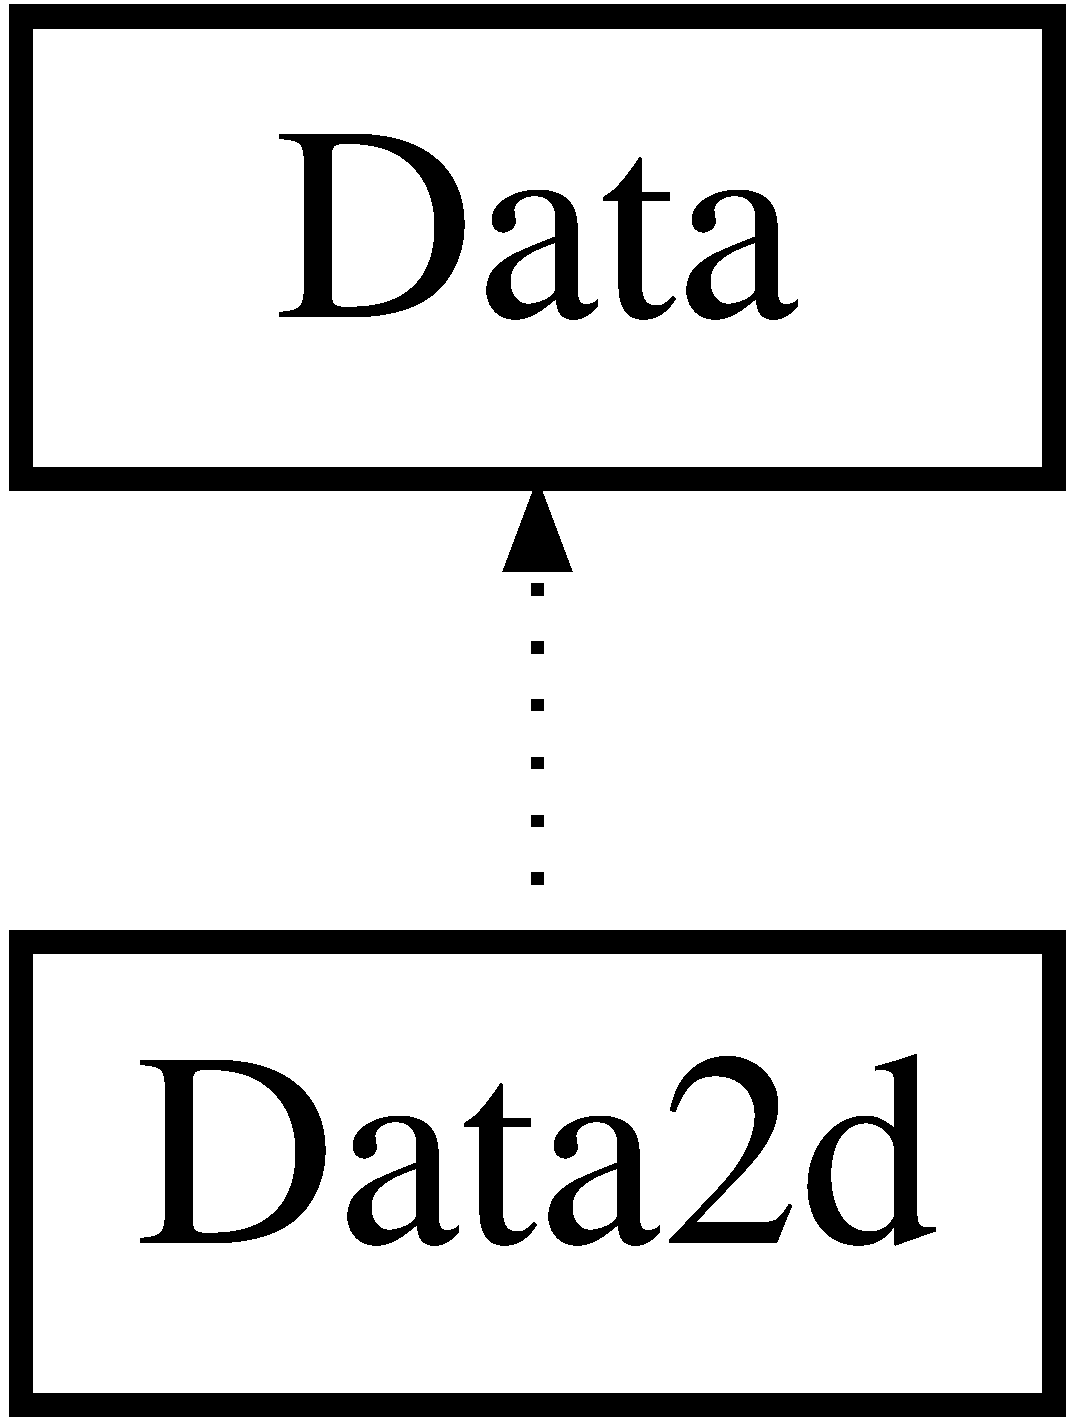
\includegraphics[height=2.000000cm]{class_data2d}
\end{center}
\end{figure}


\subsection{Detailed Description}


Definition at line 66 of file Data\+\_\+\+Generator.\+h.



The documentation for this class was generated from the following file\+:\begin{DoxyCompactItemize}
\item 
C\+:/cygwin64/home/ez pawn/\+Projects, simulation, and code/\+S\+I\+T\+S/\+Data\+\_\+\+Generator/\hyperlink{_data___generator_8h}{Data\+\_\+\+Generator.\+h}\end{DoxyCompactItemize}

\hypertarget{class_data_generator}{}\section{Data\+Generator Class Reference}
\label{class_data_generator}\index{Data\+Generator@{Data\+Generator}}


{\ttfamily \#include $<$Data\+\_\+\+Generator.\+h$>$}

Inheritance diagram for Data\+Generator\+:\begin{figure}[H]
\begin{center}
\leavevmode
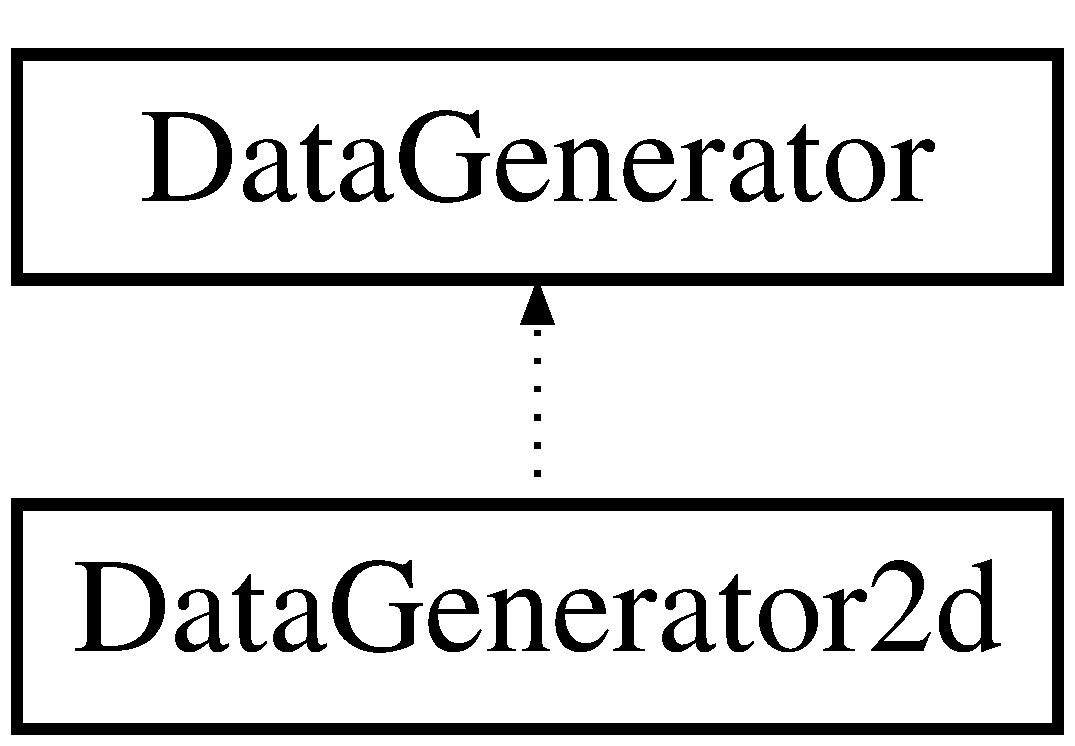
\includegraphics[height=2.000000cm]{class_data_generator}
\end{center}
\end{figure}


\subsection{Detailed Description}


Definition at line 4 of file Data\+\_\+\+Generator.\+h.



The documentation for this class was generated from the following file\+:\begin{DoxyCompactItemize}
\item 
C\+:/cygwin64/home/ez pawn/\+Projects, simulation, and code/\+S\+I\+T\+S/\+Data\+\_\+\+Generator/\hyperlink{_data___generator_8h}{Data\+\_\+\+Generator.\+h}\end{DoxyCompactItemize}

\hypertarget{class_data_generator2d}{}\section{Data\+Generator2d Class Reference}
\label{class_data_generator2d}\index{Data\+Generator2d@{Data\+Generator2d}}


!!!!!!!!!!!!!!!!!!!!!!!!!!!!!!!!!!!!!!!!!!!!!!!!!!!!!!!//  




{\ttfamily \#include $<$Data\+\_\+\+Generator.\+h$>$}

Inheritance diagram for Data\+Generator2d\+:\begin{figure}[H]
\begin{center}
\leavevmode
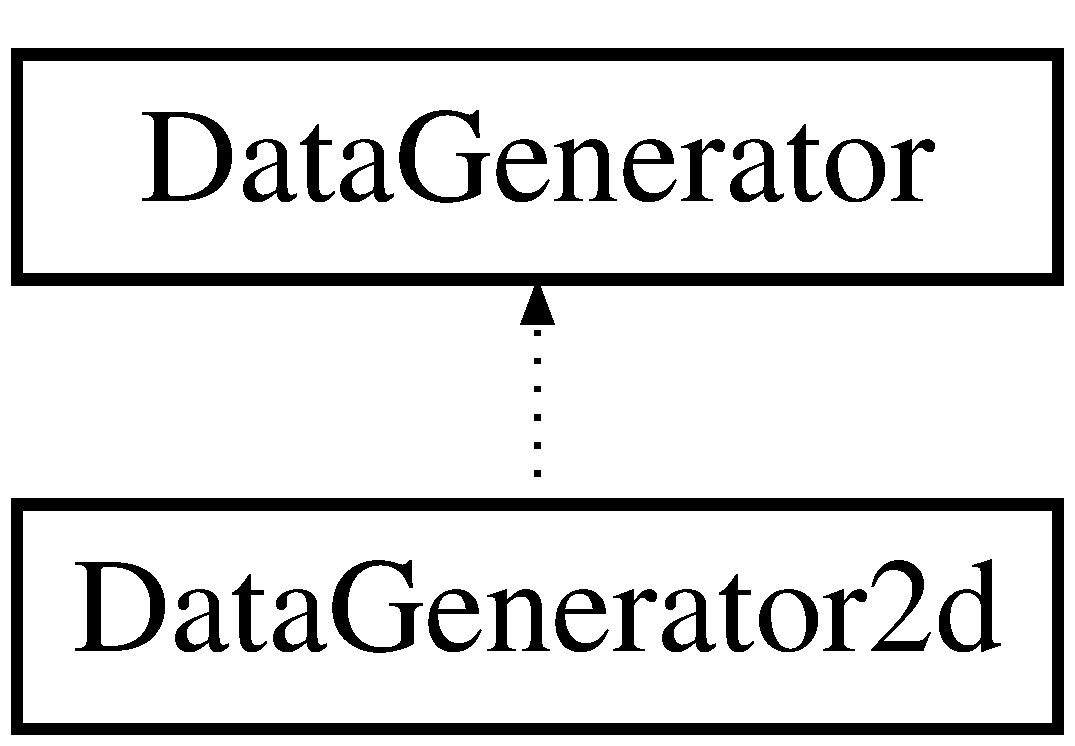
\includegraphics[height=2.000000cm]{class_data_generator2d}
\end{center}
\end{figure}


\subsection{Detailed Description}
!!!!!!!!!!!!!!!!!!!!!!!!!!!!!!!!!!!!!!!!!!!!!!!!!!!!!!!// 

Definition at line 34 of file Data\+\_\+\+Generator.\+h.



The documentation for this class was generated from the following file\+:\begin{DoxyCompactItemize}
\item 
C\+:/cygwin64/home/ez pawn/\+Projects, simulation, and code/\+S\+I\+T\+S/\+Data\+\_\+\+Generator/\hyperlink{_data___generator_8h}{Data\+\_\+\+Generator.\+h}\end{DoxyCompactItemize}

\hypertarget{class_data_manifold}{}\section{Data\+Manifold Class Reference}
\label{class_data_manifold}\index{Data\+Manifold@{Data\+Manifold}}


{\ttfamily \#include $<$Data\+\_\+\+Generator.\+h$>$}



\subsection{Detailed Description}


Definition at line 82 of file Data\+\_\+\+Generator.\+h.



The documentation for this class was generated from the following file\+:\begin{DoxyCompactItemize}
\item 
C\+:/cygwin64/home/ez pawn/\+Projects, simulation, and code/\+S\+I\+T\+S/\+Data\+\_\+\+Generator/\hyperlink{_data___generator_8h}{Data\+\_\+\+Generator.\+h}\end{DoxyCompactItemize}

\hypertarget{class_field}{}\section{Field Class Reference}
\label{class_field}\index{Field@{Field}}


{\ttfamily \#include $<$Data\+\_\+\+Generator.\+h$>$}



\subsection{Detailed Description}


Definition at line 86 of file Data\+\_\+\+Generator.\+h.



The documentation for this class was generated from the following file\+:\begin{DoxyCompactItemize}
\item 
C\+:/cygwin64/home/ez pawn/\+Projects, simulation, and code/\+S\+I\+T\+S/\+Data\+\_\+\+Generator/\hyperlink{_data___generator_8h}{Data\+\_\+\+Generator.\+h}\end{DoxyCompactItemize}

\hypertarget{classpoint}{}\section{point Class Reference}
\label{classpoint}\index{point@{point}}


{\ttfamily \#include $<$Prototypes.\+h$>$}

\subsection*{Public Member Functions}
\begin{DoxyCompactItemize}
\item 
void \hyperlink{classpoint_a55ff7a33caa2783f318bc5f65746e32e}{set} (double xp, double yp)
\item 
\hyperlink{classpoint_a5fe21d4a4539320bf0f5caf1218d31c8}{point} ()
\item 
\hyperlink{classpoint_a35a81eb47d874ab0ad36577aad5fc464}{point} (double xp, double yp)
\item 
void \hyperlink{classpoint_a55ff7a33caa2783f318bc5f65746e32e}{set} (double xp, double yp)
\item 
\hyperlink{classpoint_a5fe21d4a4539320bf0f5caf1218d31c8}{point} ()
\item 
\hyperlink{classpoint_a35a81eb47d874ab0ad36577aad5fc464}{point} (double xp, double yp)
\item 
void \hyperlink{classpoint_a55ff7a33caa2783f318bc5f65746e32e}{set} (double xp, double yp)
\item 
\hyperlink{classpoint_a5fe21d4a4539320bf0f5caf1218d31c8}{point} ()
\item 
\hyperlink{classpoint_a35a81eb47d874ab0ad36577aad5fc464}{point} (double xp, double yp)
\end{DoxyCompactItemize}
\subsection*{Public Attributes}
\begin{DoxyCompactItemize}
\item 
double \hyperlink{classpoint_a9c6b34deaf4900ad4193c17935fd384a}{x}
\item 
double \hyperlink{classpoint_a613f8f0d7352731638b0094e1b958b87}{y}
\end{DoxyCompactItemize}


\subsection{Detailed Description}


Definition at line 12 of file Prototypes.\+h.



\subsection{Constructor \& Destructor Documentation}
\mbox{\Hypertarget{classpoint_a5fe21d4a4539320bf0f5caf1218d31c8}\label{classpoint_a5fe21d4a4539320bf0f5caf1218d31c8}} 
\index{point@{point}!point@{point}}
\index{point@{point}!point@{point}}
\subsubsection{\texorpdfstring{point()}{point()}\hspace{0.1cm}{\footnotesize\ttfamily [1/6]}}
{\footnotesize\ttfamily point\+::point (\begin{DoxyParamCaption}{ }\end{DoxyParamCaption})\hspace{0.3cm}{\ttfamily [inline]}}



Definition at line 16 of file Prototypes.\+h.

\mbox{\Hypertarget{classpoint_a35a81eb47d874ab0ad36577aad5fc464}\label{classpoint_a35a81eb47d874ab0ad36577aad5fc464}} 
\index{point@{point}!point@{point}}
\index{point@{point}!point@{point}}
\subsubsection{\texorpdfstring{point()}{point()}\hspace{0.1cm}{\footnotesize\ttfamily [2/6]}}
{\footnotesize\ttfamily point\+::point (\begin{DoxyParamCaption}\item[{double}]{xp,  }\item[{double}]{yp }\end{DoxyParamCaption})\hspace{0.3cm}{\ttfamily [inline]}}



Definition at line 17 of file Prototypes.\+h.

\mbox{\Hypertarget{classpoint_a5fe21d4a4539320bf0f5caf1218d31c8}\label{classpoint_a5fe21d4a4539320bf0f5caf1218d31c8}} 
\index{point@{point}!point@{point}}
\index{point@{point}!point@{point}}
\subsubsection{\texorpdfstring{point()}{point()}\hspace{0.1cm}{\footnotesize\ttfamily [3/6]}}
{\footnotesize\ttfamily point\+::point (\begin{DoxyParamCaption}{ }\end{DoxyParamCaption})\hspace{0.3cm}{\ttfamily [inline]}}



Definition at line 25 of file Target.\+h.

\mbox{\Hypertarget{classpoint_a35a81eb47d874ab0ad36577aad5fc464}\label{classpoint_a35a81eb47d874ab0ad36577aad5fc464}} 
\index{point@{point}!point@{point}}
\index{point@{point}!point@{point}}
\subsubsection{\texorpdfstring{point()}{point()}\hspace{0.1cm}{\footnotesize\ttfamily [4/6]}}
{\footnotesize\ttfamily point\+::point (\begin{DoxyParamCaption}\item[{double}]{xp,  }\item[{double}]{yp }\end{DoxyParamCaption})\hspace{0.3cm}{\ttfamily [inline]}}



Definition at line 26 of file Target.\+h.

\mbox{\Hypertarget{classpoint_a5fe21d4a4539320bf0f5caf1218d31c8}\label{classpoint_a5fe21d4a4539320bf0f5caf1218d31c8}} 
\index{point@{point}!point@{point}}
\index{point@{point}!point@{point}}
\subsubsection{\texorpdfstring{point()}{point()}\hspace{0.1cm}{\footnotesize\ttfamily [5/6]}}
{\footnotesize\ttfamily point\+::point (\begin{DoxyParamCaption}{ }\end{DoxyParamCaption})\hspace{0.3cm}{\ttfamily [inline]}}



Definition at line 16 of file Prototypes.\+h.

\mbox{\Hypertarget{classpoint_a35a81eb47d874ab0ad36577aad5fc464}\label{classpoint_a35a81eb47d874ab0ad36577aad5fc464}} 
\index{point@{point}!point@{point}}
\index{point@{point}!point@{point}}
\subsubsection{\texorpdfstring{point()}{point()}\hspace{0.1cm}{\footnotesize\ttfamily [6/6]}}
{\footnotesize\ttfamily point\+::point (\begin{DoxyParamCaption}\item[{double}]{xp,  }\item[{double}]{yp }\end{DoxyParamCaption})\hspace{0.3cm}{\ttfamily [inline]}}



Definition at line 17 of file Prototypes.\+h.



\subsection{Member Function Documentation}
\mbox{\Hypertarget{classpoint_a55ff7a33caa2783f318bc5f65746e32e}\label{classpoint_a55ff7a33caa2783f318bc5f65746e32e}} 
\index{point@{point}!set@{set}}
\index{set@{set}!point@{point}}
\subsubsection{\texorpdfstring{set()}{set()}\hspace{0.1cm}{\footnotesize\ttfamily [1/3]}}
{\footnotesize\ttfamily void point\+::set (\begin{DoxyParamCaption}\item[{double}]{xp,  }\item[{double}]{yp }\end{DoxyParamCaption})\hspace{0.3cm}{\ttfamily [inline]}}



Definition at line 15 of file Prototypes.\+h.

\mbox{\Hypertarget{classpoint_a55ff7a33caa2783f318bc5f65746e32e}\label{classpoint_a55ff7a33caa2783f318bc5f65746e32e}} 
\index{point@{point}!set@{set}}
\index{set@{set}!point@{point}}
\subsubsection{\texorpdfstring{set()}{set()}\hspace{0.1cm}{\footnotesize\ttfamily [2/3]}}
{\footnotesize\ttfamily void point\+::set (\begin{DoxyParamCaption}\item[{double}]{xp,  }\item[{double}]{yp }\end{DoxyParamCaption})\hspace{0.3cm}{\ttfamily [inline]}}



Definition at line 15 of file Prototypes.\+h.

\mbox{\Hypertarget{classpoint_a55ff7a33caa2783f318bc5f65746e32e}\label{classpoint_a55ff7a33caa2783f318bc5f65746e32e}} 
\index{point@{point}!set@{set}}
\index{set@{set}!point@{point}}
\subsubsection{\texorpdfstring{set()}{set()}\hspace{0.1cm}{\footnotesize\ttfamily [3/3]}}
{\footnotesize\ttfamily void point\+::set (\begin{DoxyParamCaption}\item[{double}]{xp,  }\item[{double}]{yp }\end{DoxyParamCaption})\hspace{0.3cm}{\ttfamily [inline]}}



Definition at line 24 of file Target.\+h.



\subsection{Member Data Documentation}
\mbox{\Hypertarget{classpoint_a9c6b34deaf4900ad4193c17935fd384a}\label{classpoint_a9c6b34deaf4900ad4193c17935fd384a}} 
\index{point@{point}!x@{x}}
\index{x@{x}!point@{point}}
\subsubsection{\texorpdfstring{x}{x}}
{\footnotesize\ttfamily double point\+::x}



Definition at line 14 of file Prototypes.\+h.

\mbox{\Hypertarget{classpoint_a613f8f0d7352731638b0094e1b958b87}\label{classpoint_a613f8f0d7352731638b0094e1b958b87}} 
\index{point@{point}!y@{y}}
\index{y@{y}!point@{point}}
\subsubsection{\texorpdfstring{y}{y}}
{\footnotesize\ttfamily double point\+::y}



Definition at line 14 of file Prototypes.\+h.



The documentation for this class was generated from the following files\+:\begin{DoxyCompactItemize}
\item 
C\+:/cygwin64/home/ez pawn/\+Projects, simulation, and code/\+S\+I\+T\+S/\+Data\+\_\+\+Generator/\hyperlink{_data___generator_2_prototypes_8h}{Prototypes.\+h}\item 
C\+:/cygwin64/home/ez pawn/\+Projects, simulation, and code/\+S\+I\+T\+S/lib/\hyperlink{_target_8h}{Target.\+h}\end{DoxyCompactItemize}

\hypertarget{class_target}{}\section{Target Class Reference}
\label{class_target}\index{Target@{Target}}


{\ttfamily \#include $<$Target.\+h$>$}



\subsection{Detailed Description}
A target represents a physical entity that we would scatter an incident field. Curently, targets are assumed stationary. Should relax this latter. Subclasses include sampled targets, and function targets. A function target takes in a point and returns the reflectivity at that point. 

Definition at line 8 of file Target.\+h.



The documentation for this class was generated from the following file\+:\begin{DoxyCompactItemize}
\item 
C\+:/cygwin64/home/ez pawn/\+Projects, simulation, and code/\+S\+I\+T\+S/lib/\hyperlink{_target_8h}{Target.\+h}\end{DoxyCompactItemize}

\hypertarget{class_target2d_f}{}\section{Target2dF Class Reference}
\label{class_target2d_f}\index{Target2dF@{Target2dF}}


{\ttfamily \#include $<$Target.\+h$>$}



\subsection{Detailed Description}


Definition at line 39 of file Target.\+h.



The documentation for this class was generated from the following file\+:\begin{DoxyCompactItemize}
\item 
C\+:/cygwin64/home/ez pawn/\+Projects, simulation, and code/\+S\+I\+T\+S/lib/\hyperlink{_target_8h}{Target.\+h}\end{DoxyCompactItemize}

\hypertarget{class_target2d_s}{}\section{Target2dS Class Reference}
\label{class_target2d_s}\index{Target2dS@{Target2dS}}


{\ttfamily \#include $<$Target.\+h$>$}



\subsection{Detailed Description}


Definition at line 35 of file Target.\+h.



The documentation for this class was generated from the following file\+:\begin{DoxyCompactItemize}
\item 
C\+:/cygwin64/home/ez pawn/\+Projects, simulation, and code/\+S\+I\+T\+S/lib/\hyperlink{_target_8h}{Target.\+h}\end{DoxyCompactItemize}

\hypertarget{class_target3d_s}{}\section{Target3dS Class Reference}
\label{class_target3d_s}\index{Target3dS@{Target3dS}}


{\ttfamily \#include $<$Target.\+h$>$}



\subsection{Detailed Description}


Definition at line 37 of file Target.\+h.



The documentation for this class was generated from the following file\+:\begin{DoxyCompactItemize}
\item 
C\+:/cygwin64/home/ez pawn/\+Projects, simulation, and code/\+S\+I\+T\+S/lib/\hyperlink{_target_8h}{Target.\+h}\end{DoxyCompactItemize}

\chapter{File Documentation}
\hypertarget{_data___generator_8cpp}{}\section{C\+:/cygwin64/home/ez pawn/\+Projects, simulation, and code/\+S\+I\+T\+S/\+Data\+\_\+\+Generator/\+Data\+\_\+\+Generator.cpp File Reference}
\label{_data___generator_8cpp}\index{C\+:/cygwin64/home/ez pawn/\+Projects, simulation, and code/\+S\+I\+T\+S/\+Data\+\_\+\+Generator/\+Data\+\_\+\+Generator.\+cpp@{C\+:/cygwin64/home/ez pawn/\+Projects, simulation, and code/\+S\+I\+T\+S/\+Data\+\_\+\+Generator/\+Data\+\_\+\+Generator.\+cpp}}
{\ttfamily \#include \char`\"{}Data\+\_\+\+Generator.\+h\char`\"{}}\newline
\subsection*{Functions}
\begin{DoxyCompactItemize}
\item 
int \hyperlink{_data___generator_8cpp_a0ddf1224851353fc92bfbff6f499fa97}{main} (int argc, char $\ast$argv\mbox{[}$\,$\mbox{]})
\end{DoxyCompactItemize}


\subsection{Function Documentation}
\mbox{\Hypertarget{_data___generator_8cpp_a0ddf1224851353fc92bfbff6f499fa97}\label{_data___generator_8cpp_a0ddf1224851353fc92bfbff6f499fa97}} 
\index{Data\+\_\+\+Generator.\+cpp@{Data\+\_\+\+Generator.\+cpp}!main@{main}}
\index{main@{main}!Data\+\_\+\+Generator.\+cpp@{Data\+\_\+\+Generator.\+cpp}}
\subsubsection{\texorpdfstring{main()}{main()}}
{\footnotesize\ttfamily int main (\begin{DoxyParamCaption}\item[{int}]{argc,  }\item[{char $\ast$}]{argv\mbox{[}$\,$\mbox{]} }\end{DoxyParamCaption})}



Definition at line 9 of file Data\+\_\+\+Generator.\+cpp.


\hypertarget{_data___generator_8h}{}\section{C\+:/cygwin64/home/ez pawn/\+Projects, simulation, and code/\+S\+I\+T\+S/\+Data\+\_\+\+Generator/\+Data\+\_\+\+Generator.h File Reference}
\label{_data___generator_8h}\index{C\+:/cygwin64/home/ez pawn/\+Projects, simulation, and code/\+S\+I\+T\+S/\+Data\+\_\+\+Generator/\+Data\+\_\+\+Generator.\+h@{C\+:/cygwin64/home/ez pawn/\+Projects, simulation, and code/\+S\+I\+T\+S/\+Data\+\_\+\+Generator/\+Data\+\_\+\+Generator.\+h}}
{\ttfamily \#include \char`\"{}input.\+h\char`\"{}}\newline
\subsection*{Classes}
\begin{DoxyCompactItemize}
\item 
class \hyperlink{class_data_generator}{Data\+Generator}
\item 
class \hyperlink{class_data_generator2d}{Data\+Generator2d}
\begin{DoxyCompactList}\small\item\em !!!!!!!!!!!!!!!!!!!!!!!!!!!!!!!!!!!!!!!!!!!!!!!!!!!!!!!// \end{DoxyCompactList}\item 
class \hyperlink{class_data2d}{Data2d}
\item 
class \hyperlink{class_data_manifold}{Data\+Manifold}
\item 
class \hyperlink{class_field}{Field}
\end{DoxyCompactItemize}
\subsection*{Functions}
\begin{DoxyCompactItemize}
\item 
int \hyperlink{_data___generator_8h_a325b4b80c42799ef04293ca89c91a8ec}{Field\+\_\+\+On\+\_\+\+Support\+\_\+\+Index} (int s, int w, int j)
\begin{DoxyCompactList}\small\item\em !!!!!!\+Functions to data Generation!!!!!!!!!!!!!!!!!!!!!// \end{DoxyCompactList}\item 
void \hyperlink{_data___generator_8h_a108bf510bc5bb509c831922e9c798eb8}{Read\+\_\+\+In\+\_\+\+Reflectivity} (double $\ast$reflectivity, string file)
\item 
int \hyperlink{_data___generator_8h_a79dbb3fdf60711e80d51c0c0c562e5f8}{Size\+\_\+\+Of\+\_\+\+Support} (double $\ast$reflectivity)
\item 
complex$<$ double $>$ \hyperlink{_data___generator_8h_a398a71365b23d1c040265d5533776c01}{Incident\+\_\+\+Field} (int s, int w, double x, double y)
\item 
double \hyperlink{_data___generator_8h_a7bda372c140e2175bfb8c5f407a3fa6f}{Norm} (double x, double y, double z)
\item 
complex$<$ double $>$ \hyperlink{_data___generator_8h_a974c700eb23491a012ceeab54d82cdc2}{G} (double x, double y, double z, double w)
\item 
complex$<$ double $>$ \hyperlink{_data___generator_8h_ae42eb598125814cc2888d4eadd7a04f8}{Scattered\+\_\+\+Field\+\_\+\+At\+\_\+\+Point} (double x, double y, int w, int s, double $\ast$reflectivity, complex$<$ double $>$ $\ast$field\+\_\+on\+\_\+target\+\_\+support, int \hyperlink{_target___generator_2_prototypes_8h_a788d8695493e8fbe8a998049de220e25}{S})
\item 
complex$<$ double $>$ $\ast$ \hyperlink{_data___generator_8h_ac94ea0064b7e3823260dba9d5e91e2fa}{Generate\+\_\+\+Data} (double $\ast$reflectivity, int \hyperlink{_target___generator_2_input_8h_a7b63ccc35ac484b9f41e37ccd0cb31bd}{K})
\item 
void \hyperlink{_data___generator_8h_af552c71b8dfb2ef0f79eabc0025de558}{Output\+\_\+\+Data} (complex$<$ double $>$ $\ast$data, string file\+\_\+name)
\item 
\hyperlink{class_data2d}{Data2d} Data \hyperlink{_data___generator_8h_a5ee4670d3ae00ec99f8297e10f0a6467}{flight\+\_\+path} (float t)
\item 
void \hyperlink{_data___generator_8h_a8f082dd9626b5a1fb97fba5a6c236fb1}{Generate\+\_\+\+Data} (string infilename)
\end{DoxyCompactItemize}
\subsection*{Variables}
\begin{DoxyCompactItemize}
\item 
\hyperlink{class_data_generator2d}{Data\+Generator2d} \hyperlink{_data___generator_8h_aeb7bb2aca60ddfc3124525269662df7a}{format} =\char`\"{}R\+AW\char`\"{}
\item 
point2d class \hyperlink{class_data_manifold}{Data\+Manifold} \hyperlink{_data___generator_8h_a38ad8d1091246bf456114eac49a0757f}{flight\+\_\+path}
\end{DoxyCompactItemize}


\subsection{Function Documentation}
\mbox{\Hypertarget{_data___generator_8h_a325b4b80c42799ef04293ca89c91a8ec}\label{_data___generator_8h_a325b4b80c42799ef04293ca89c91a8ec}} 
\index{Data\+\_\+\+Generator.\+h@{Data\+\_\+\+Generator.\+h}!Field\+\_\+\+On\+\_\+\+Support\+\_\+\+Index@{Field\+\_\+\+On\+\_\+\+Support\+\_\+\+Index}}
\index{Field\+\_\+\+On\+\_\+\+Support\+\_\+\+Index@{Field\+\_\+\+On\+\_\+\+Support\+\_\+\+Index}!Data\+\_\+\+Generator.\+h@{Data\+\_\+\+Generator.\+h}}
\subsubsection{\texorpdfstring{Field\+\_\+\+On\+\_\+\+Support\+\_\+\+Index()}{Field\_On\_Support\_Index()}}
{\footnotesize\ttfamily int Field\+\_\+\+On\+\_\+\+Support\+\_\+\+Index (\begin{DoxyParamCaption}\item[{int}]{s,  }\item[{int}]{w,  }\item[{int}]{j }\end{DoxyParamCaption})\hspace{0.3cm}{\ttfamily [inline]}}



!!!!!!\+Functions to data Generation!!!!!!!!!!!!!!!!!!!!!// 

\mbox{\Hypertarget{_data___generator_8h_a5ee4670d3ae00ec99f8297e10f0a6467}\label{_data___generator_8h_a5ee4670d3ae00ec99f8297e10f0a6467}} 
\index{Data\+\_\+\+Generator.\+h@{Data\+\_\+\+Generator.\+h}!flight\+\_\+path@{flight\+\_\+path}}
\index{flight\+\_\+path@{flight\+\_\+path}!Data\+\_\+\+Generator.\+h@{Data\+\_\+\+Generator.\+h}}
\subsubsection{\texorpdfstring{flight\+\_\+path()}{flight\_path()}}
{\footnotesize\ttfamily \hyperlink{class_data2d}{Data2d} Data flight\+\_\+path (\begin{DoxyParamCaption}\item[{float}]{t }\end{DoxyParamCaption})}

A S\+AR is a system that has a moving antenna which coherently \mbox{\Hypertarget{_data___generator_8h_a974c700eb23491a012ceeab54d82cdc2}\label{_data___generator_8h_a974c700eb23491a012ceeab54d82cdc2}} 
\index{Data\+\_\+\+Generator.\+h@{Data\+\_\+\+Generator.\+h}!G@{G}}
\index{G@{G}!Data\+\_\+\+Generator.\+h@{Data\+\_\+\+Generator.\+h}}
\subsubsection{\texorpdfstring{G()}{G()}}
{\footnotesize\ttfamily complex$<$double$>$ G (\begin{DoxyParamCaption}\item[{double}]{x,  }\item[{double}]{y,  }\item[{double}]{z,  }\item[{double}]{w }\end{DoxyParamCaption})\hspace{0.3cm}{\ttfamily [inline]}}



Definition at line 33 of file Input.\+h.

\mbox{\Hypertarget{_data___generator_8h_ac94ea0064b7e3823260dba9d5e91e2fa}\label{_data___generator_8h_ac94ea0064b7e3823260dba9d5e91e2fa}} 
\index{Data\+\_\+\+Generator.\+h@{Data\+\_\+\+Generator.\+h}!Generate\+\_\+\+Data@{Generate\+\_\+\+Data}}
\index{Generate\+\_\+\+Data@{Generate\+\_\+\+Data}!Data\+\_\+\+Generator.\+h@{Data\+\_\+\+Generator.\+h}}
\subsubsection{\texorpdfstring{Generate\+\_\+\+Data()}{Generate\_Data()}\hspace{0.1cm}{\footnotesize\ttfamily [1/2]}}
{\footnotesize\ttfamily complex$<$double$>$$\ast$ Generate\+\_\+\+Data (\begin{DoxyParamCaption}\item[{double $\ast$}]{reflectivity,  }\item[{int}]{K }\end{DoxyParamCaption})}

\mbox{\Hypertarget{_data___generator_8h_a8f082dd9626b5a1fb97fba5a6c236fb1}\label{_data___generator_8h_a8f082dd9626b5a1fb97fba5a6c236fb1}} 
\index{Data\+\_\+\+Generator.\+h@{Data\+\_\+\+Generator.\+h}!Generate\+\_\+\+Data@{Generate\+\_\+\+Data}}
\index{Generate\+\_\+\+Data@{Generate\+\_\+\+Data}!Data\+\_\+\+Generator.\+h@{Data\+\_\+\+Generator.\+h}}
\subsubsection{\texorpdfstring{Generate\+\_\+\+Data()}{Generate\_Data()}\hspace{0.1cm}{\footnotesize\ttfamily [2/2]}}
{\footnotesize\ttfamily void Generate\+\_\+\+Data (\begin{DoxyParamCaption}\item[{string}]{infilename }\end{DoxyParamCaption})}



Definition at line 206 of file Data\+\_\+\+Generator.\+h.

\mbox{\Hypertarget{_data___generator_8h_a398a71365b23d1c040265d5533776c01}\label{_data___generator_8h_a398a71365b23d1c040265d5533776c01}} 
\index{Data\+\_\+\+Generator.\+h@{Data\+\_\+\+Generator.\+h}!Incident\+\_\+\+Field@{Incident\+\_\+\+Field}}
\index{Incident\+\_\+\+Field@{Incident\+\_\+\+Field}!Data\+\_\+\+Generator.\+h@{Data\+\_\+\+Generator.\+h}}
\subsubsection{\texorpdfstring{Incident\+\_\+\+Field()}{Incident\_Field()}}
{\footnotesize\ttfamily complex$<$double$>$ Incident\+\_\+\+Field (\begin{DoxyParamCaption}\item[{int}]{s,  }\item[{int}]{w,  }\item[{double}]{x,  }\item[{double}]{y }\end{DoxyParamCaption})}

\mbox{\Hypertarget{_data___generator_8h_a7bda372c140e2175bfb8c5f407a3fa6f}\label{_data___generator_8h_a7bda372c140e2175bfb8c5f407a3fa6f}} 
\index{Data\+\_\+\+Generator.\+h@{Data\+\_\+\+Generator.\+h}!Norm@{Norm}}
\index{Norm@{Norm}!Data\+\_\+\+Generator.\+h@{Data\+\_\+\+Generator.\+h}}
\subsubsection{\texorpdfstring{Norm()}{Norm()}}
{\footnotesize\ttfamily double Norm (\begin{DoxyParamCaption}\item[{double}]{x,  }\item[{double}]{y,  }\item[{double}]{z }\end{DoxyParamCaption})\hspace{0.3cm}{\ttfamily [inline]}}



Definition at line 37 of file Input.\+h.

\mbox{\Hypertarget{_data___generator_8h_af552c71b8dfb2ef0f79eabc0025de558}\label{_data___generator_8h_af552c71b8dfb2ef0f79eabc0025de558}} 
\index{Data\+\_\+\+Generator.\+h@{Data\+\_\+\+Generator.\+h}!Output\+\_\+\+Data@{Output\+\_\+\+Data}}
\index{Output\+\_\+\+Data@{Output\+\_\+\+Data}!Data\+\_\+\+Generator.\+h@{Data\+\_\+\+Generator.\+h}}
\subsubsection{\texorpdfstring{Output\+\_\+\+Data()}{Output\_Data()}}
{\footnotesize\ttfamily void Output\+\_\+\+Data (\begin{DoxyParamCaption}\item[{complex$<$ double $>$ $\ast$}]{data,  }\item[{string}]{file\+\_\+name }\end{DoxyParamCaption})\hspace{0.3cm}{\ttfamily [inline]}}

\mbox{\Hypertarget{_data___generator_8h_a108bf510bc5bb509c831922e9c798eb8}\label{_data___generator_8h_a108bf510bc5bb509c831922e9c798eb8}} 
\index{Data\+\_\+\+Generator.\+h@{Data\+\_\+\+Generator.\+h}!Read\+\_\+\+In\+\_\+\+Reflectivity@{Read\+\_\+\+In\+\_\+\+Reflectivity}}
\index{Read\+\_\+\+In\+\_\+\+Reflectivity@{Read\+\_\+\+In\+\_\+\+Reflectivity}!Data\+\_\+\+Generator.\+h@{Data\+\_\+\+Generator.\+h}}
\subsubsection{\texorpdfstring{Read\+\_\+\+In\+\_\+\+Reflectivity()}{Read\_In\_Reflectivity()}}
{\footnotesize\ttfamily void Read\+\_\+\+In\+\_\+\+Reflectivity (\begin{DoxyParamCaption}\item[{double $\ast$}]{reflectivity,  }\item[{string}]{file }\end{DoxyParamCaption})}

\mbox{\Hypertarget{_data___generator_8h_ae42eb598125814cc2888d4eadd7a04f8}\label{_data___generator_8h_ae42eb598125814cc2888d4eadd7a04f8}} 
\index{Data\+\_\+\+Generator.\+h@{Data\+\_\+\+Generator.\+h}!Scattered\+\_\+\+Field\+\_\+\+At\+\_\+\+Point@{Scattered\+\_\+\+Field\+\_\+\+At\+\_\+\+Point}}
\index{Scattered\+\_\+\+Field\+\_\+\+At\+\_\+\+Point@{Scattered\+\_\+\+Field\+\_\+\+At\+\_\+\+Point}!Data\+\_\+\+Generator.\+h@{Data\+\_\+\+Generator.\+h}}
\subsubsection{\texorpdfstring{Scattered\+\_\+\+Field\+\_\+\+At\+\_\+\+Point()}{Scattered\_Field\_At\_Point()}}
{\footnotesize\ttfamily complex$<$double$>$ Scattered\+\_\+\+Field\+\_\+\+At\+\_\+\+Point (\begin{DoxyParamCaption}\item[{double}]{x,  }\item[{double}]{y,  }\item[{int}]{w,  }\item[{int}]{s,  }\item[{double $\ast$}]{reflectivity,  }\item[{complex$<$ double $>$ $\ast$}]{field\+\_\+on\+\_\+target\+\_\+support,  }\item[{int}]{S }\end{DoxyParamCaption})}

\mbox{\Hypertarget{_data___generator_8h_a79dbb3fdf60711e80d51c0c0c562e5f8}\label{_data___generator_8h_a79dbb3fdf60711e80d51c0c0c562e5f8}} 
\index{Data\+\_\+\+Generator.\+h@{Data\+\_\+\+Generator.\+h}!Size\+\_\+\+Of\+\_\+\+Support@{Size\+\_\+\+Of\+\_\+\+Support}}
\index{Size\+\_\+\+Of\+\_\+\+Support@{Size\+\_\+\+Of\+\_\+\+Support}!Data\+\_\+\+Generator.\+h@{Data\+\_\+\+Generator.\+h}}
\subsubsection{\texorpdfstring{Size\+\_\+\+Of\+\_\+\+Support()}{Size\_Of\_Support()}}
{\footnotesize\ttfamily int Size\+\_\+\+Of\+\_\+\+Support (\begin{DoxyParamCaption}\item[{double $\ast$}]{reflectivity }\end{DoxyParamCaption})}



Definition at line 43 of file Target.\+h.



\subsection{Variable Documentation}
\mbox{\Hypertarget{_data___generator_8h_a38ad8d1091246bf456114eac49a0757f}\label{_data___generator_8h_a38ad8d1091246bf456114eac49a0757f}} 
\index{Data\+\_\+\+Generator.\+h@{Data\+\_\+\+Generator.\+h}!flight\+\_\+path@{flight\+\_\+path}}
\index{flight\+\_\+path@{flight\+\_\+path}!Data\+\_\+\+Generator.\+h@{Data\+\_\+\+Generator.\+h}}
\subsubsection{\texorpdfstring{flight\+\_\+path}{flight\_path}}
{\footnotesize\ttfamily point2d class \hyperlink{class_data_manifold}{Data\+Manifold} flight\+\_\+path}

\mbox{\Hypertarget{_data___generator_8h_aeb7bb2aca60ddfc3124525269662df7a}\label{_data___generator_8h_aeb7bb2aca60ddfc3124525269662df7a}} 
\index{Data\+\_\+\+Generator.\+h@{Data\+\_\+\+Generator.\+h}!format@{format}}
\index{format@{format}!Data\+\_\+\+Generator.\+h@{Data\+\_\+\+Generator.\+h}}
\subsubsection{\texorpdfstring{format}{format}}
{\footnotesize\ttfamily  \hyperlink{class_data_generator2d}{Data\+Generator2d} format =\char`\"{}R\+AW\char`\"{}}


\hypertarget{_data___generator_2_input_8h}{}\section{C\+:/cygwin64/home/ez pawn/\+Projects, simulation, and code/\+S\+I\+T\+S/\+Data\+\_\+\+Generator/\+Input.h File Reference}
\label{_data___generator_2_input_8h}\index{C\+:/cygwin64/home/ez pawn/\+Projects, simulation, and code/\+S\+I\+T\+S/\+Data\+\_\+\+Generator/\+Input.\+h@{C\+:/cygwin64/home/ez pawn/\+Projects, simulation, and code/\+S\+I\+T\+S/\+Data\+\_\+\+Generator/\+Input.\+h}}
{\ttfamily \#include \char`\"{}prototypes.\+h\char`\"{}}\newline
\subsection*{Functions}
\begin{DoxyCompactItemize}
\item 
const complex$<$ double $>$ \hyperlink{_data___generator_2_input_8h_a5d6816662449d5e74ab1f78234044260}{i} (0, 1)
\item 
complex$<$ double $>$ \hyperlink{_data___generator_2_input_8h_a974c700eb23491a012ceeab54d82cdc2}{G} (double x, double y, double z, double w)
\item 
double \hyperlink{_data___generator_2_input_8h_a7bda372c140e2175bfb8c5f407a3fa6f}{Norm} (double x, double y, double z)
\item 
double \hyperlink{_data___generator_2_input_8h_a285206837634162341a856a6e2cf8594}{Gamma\+\_\+X} (double s)
\item 
double \hyperlink{_data___generator_2_input_8h_a12a050b07dfebcf7bd1a42b264e56d10}{Gamma\+\_\+Y} (double s)
\item 
double \hyperlink{_data___generator_2_input_8h_a748e17292f693395243fe998c44ed79f}{phi} (\hyperlink{classpoint}{point} x, \hyperlink{classpoint}{point} y)
\item 
complex$<$ double $>$ \hyperlink{_data___generator_2_input_8h_a1518bf2507ae0de796462fe244a92884}{interp} (complex$<$ double $>$ $\ast$d, double sl, double qj)
\item 
complex$<$ double $>$ \hyperlink{_data___generator_2_input_8h_abe8880126524e4cd8a95094d7e70c4d7}{p} (double w)
\item 
complex$<$ double $>$ \hyperlink{_data___generator_2_input_8h_ad28d23d18460a766bace637017e0ffae}{f} (\hyperlink{classpoint}{point} y, complex$<$ double $>$ $\ast$d)
\begin{DoxyCompactList}\small\item\em !!!!!!!!!!!!!!!!!!!!!!!!!!!!!!!!!!!!!!!!!!!!!!!!!!!!!!!!!!!!// \end{DoxyCompactList}\end{DoxyCompactItemize}
\subsection*{Variables}
\begin{DoxyCompactItemize}
\item 
const double \hyperlink{_data___generator_2_input_8h_a43016d873124d39034edb8cd164794db}{pi} =3.\+14159265359
\item 
const double \hyperlink{_data___generator_2_input_8h_a238dd1656c08db3032dac4e8933ec29f}{c\+\_\+0} =299792458
\item 
const int \hyperlink{_data___generator_2_input_8h_ab2b6b0c222cd1ce70d6a831f57241e59}{N} =4
\item 
const int \hyperlink{_data___generator_2_input_8h_a9edc6895d567e0ddcdd3cc20df3f3b4b}{M} =\hyperlink{_target___generator_2_input_8h_ab2b6b0c222cd1ce70d6a831f57241e59}{N}$\ast$\hyperlink{_target___generator_2_input_8h_ab2b6b0c222cd1ce70d6a831f57241e59}{N}
\item 
const int \hyperlink{_data___generator_2_input_8h_a7b63ccc35ac484b9f41e37ccd0cb31bd}{K} =1
\item 
const double \hyperlink{_data___generator_2_input_8h_a4bd7627e0aadee4ba01eb37bd6aba189}{w\+\_\+0} =pow(10,9)
\item 
const double \hyperlink{_data___generator_2_input_8h_a00bd6d4b694fffd16f81568e37e472ce}{Band} =pow(10,8)
\item 
const double \hyperlink{_data___generator_2_input_8h_acb8f4382cb1ad7ce2fa9c630560a7332}{r} =100
\item 
const double \hyperlink{_data___generator_2_input_8h_ad7cd26dc1ce30ff209c71b309a3134e6}{H} =100
\item 
const int \hyperlink{_data___generator_2_input_8h_a134246d2225c23551060597d5460bd7c}{L} =log2(\hyperlink{_target___generator_2_input_8h_ab2b6b0c222cd1ce70d6a831f57241e59}{N})
\item 
const int \hyperlink{_data___generator_2_input_8h_a553198f5b4ae6b71d0a514272e1f8e21}{q} =16
\item 
const int \hyperlink{_data___generator_2_input_8h_a1084a241e9587c77068a6baf9ad9f0c6}{r\+\_\+eps} =\hyperlink{_target___generator_2_input_8h_a553198f5b4ae6b71d0a514272e1f8e21}{q}$\ast$\hyperlink{_target___generator_2_input_8h_a553198f5b4ae6b71d0a514272e1f8e21}{q}
\item 
const double \hyperlink{_data___generator_2_input_8h_a96d9e72424bb3750a125bc08bba688ff}{image\+\_\+height} =0
\item 
const int \hyperlink{_data___generator_2_input_8h_aabaa1bd1eed76e739bbc16c7e4e72549}{P} =\hyperlink{_target___generator_2_input_8h_ab2b6b0c222cd1ce70d6a831f57241e59}{N}$\ast$\hyperlink{_target___generator_2_input_8h_ab2b6b0c222cd1ce70d6a831f57241e59}{N}$\ast$\hyperlink{_target___generator_2_input_8h_a553198f5b4ae6b71d0a514272e1f8e21}{q}$\ast$\hyperlink{_target___generator_2_input_8h_a553198f5b4ae6b71d0a514272e1f8e21}{q}
\item 
const string \hyperlink{_data___generator_2_input_8h_ae481aa99ddc0fb8a143ff9c561df47a9}{filename} =\char`\"{}Easy\char`\"{}
\end{DoxyCompactItemize}


\subsection{Function Documentation}
\mbox{\Hypertarget{_data___generator_2_input_8h_ad28d23d18460a766bace637017e0ffae}\label{_data___generator_2_input_8h_ad28d23d18460a766bace637017e0ffae}} 
\index{Data\+\_\+\+Generator/\+Input.\+h@{Data\+\_\+\+Generator/\+Input.\+h}!f@{f}}
\index{f@{f}!Data\+\_\+\+Generator/\+Input.\+h@{Data\+\_\+\+Generator/\+Input.\+h}}
\subsubsection{\texorpdfstring{f()}{f()}}
{\footnotesize\ttfamily complex$<$double$>$ f (\begin{DoxyParamCaption}\item[{\hyperlink{classpoint}{point}}]{y,  }\item[{complex$<$ double $>$ $\ast$}]{d }\end{DoxyParamCaption})}



!!!!!!!!!!!!!!!!!!!!!!!!!!!!!!!!!!!!!!!!!!!!!!!!!!!!!!!!!!!!// 

!!!!!!!!!!!!!!!!!!\+Input functions!!!!!!!!!!!!!!!!!!!!!!!!!!!// 

Definition at line 71 of file Input.\+h.

\mbox{\Hypertarget{_data___generator_2_input_8h_a974c700eb23491a012ceeab54d82cdc2}\label{_data___generator_2_input_8h_a974c700eb23491a012ceeab54d82cdc2}} 
\index{Data\+\_\+\+Generator/\+Input.\+h@{Data\+\_\+\+Generator/\+Input.\+h}!G@{G}}
\index{G@{G}!Data\+\_\+\+Generator/\+Input.\+h@{Data\+\_\+\+Generator/\+Input.\+h}}
\subsubsection{\texorpdfstring{G()}{G()}}
{\footnotesize\ttfamily complex$<$double$>$ G (\begin{DoxyParamCaption}\item[{double}]{x,  }\item[{double}]{y,  }\item[{double}]{z,  }\item[{double}]{w }\end{DoxyParamCaption})\hspace{0.3cm}{\ttfamily [inline]}}



Definition at line 33 of file Input.\+h.

\mbox{\Hypertarget{_data___generator_2_input_8h_a285206837634162341a856a6e2cf8594}\label{_data___generator_2_input_8h_a285206837634162341a856a6e2cf8594}} 
\index{Data\+\_\+\+Generator/\+Input.\+h@{Data\+\_\+\+Generator/\+Input.\+h}!Gamma\+\_\+X@{Gamma\+\_\+X}}
\index{Gamma\+\_\+X@{Gamma\+\_\+X}!Data\+\_\+\+Generator/\+Input.\+h@{Data\+\_\+\+Generator/\+Input.\+h}}
\subsubsection{\texorpdfstring{Gamma\+\_\+\+X()}{Gamma\_X()}}
{\footnotesize\ttfamily double Gamma\+\_\+X (\begin{DoxyParamCaption}\item[{double}]{s }\end{DoxyParamCaption})}



Definition at line 41 of file Input.\+h.

\mbox{\Hypertarget{_data___generator_2_input_8h_a12a050b07dfebcf7bd1a42b264e56d10}\label{_data___generator_2_input_8h_a12a050b07dfebcf7bd1a42b264e56d10}} 
\index{Data\+\_\+\+Generator/\+Input.\+h@{Data\+\_\+\+Generator/\+Input.\+h}!Gamma\+\_\+Y@{Gamma\+\_\+Y}}
\index{Gamma\+\_\+Y@{Gamma\+\_\+Y}!Data\+\_\+\+Generator/\+Input.\+h@{Data\+\_\+\+Generator/\+Input.\+h}}
\subsubsection{\texorpdfstring{Gamma\+\_\+\+Y()}{Gamma\_Y()}}
{\footnotesize\ttfamily double Gamma\+\_\+Y (\begin{DoxyParamCaption}\item[{double}]{s }\end{DoxyParamCaption})}



Definition at line 45 of file Input.\+h.

\mbox{\Hypertarget{_data___generator_2_input_8h_a5d6816662449d5e74ab1f78234044260}\label{_data___generator_2_input_8h_a5d6816662449d5e74ab1f78234044260}} 
\index{Data\+\_\+\+Generator/\+Input.\+h@{Data\+\_\+\+Generator/\+Input.\+h}!i@{i}}
\index{i@{i}!Data\+\_\+\+Generator/\+Input.\+h@{Data\+\_\+\+Generator/\+Input.\+h}}
\subsubsection{\texorpdfstring{i()}{i()}}
{\footnotesize\ttfamily const complex$<$double$>$ i (\begin{DoxyParamCaption}\item[{0}]{,  }\item[{1}]{ }\end{DoxyParamCaption})}

\mbox{\Hypertarget{_data___generator_2_input_8h_a1518bf2507ae0de796462fe244a92884}\label{_data___generator_2_input_8h_a1518bf2507ae0de796462fe244a92884}} 
\index{Data\+\_\+\+Generator/\+Input.\+h@{Data\+\_\+\+Generator/\+Input.\+h}!interp@{interp}}
\index{interp@{interp}!Data\+\_\+\+Generator/\+Input.\+h@{Data\+\_\+\+Generator/\+Input.\+h}}
\subsubsection{\texorpdfstring{interp()}{interp()}}
{\footnotesize\ttfamily complex$<$double$>$ interp (\begin{DoxyParamCaption}\item[{complex$<$ double $>$ $\ast$}]{d,  }\item[{double}]{sl,  }\item[{double}]{qj }\end{DoxyParamCaption})}



Definition at line 56 of file Input.\+h.

\mbox{\Hypertarget{_data___generator_2_input_8h_a7bda372c140e2175bfb8c5f407a3fa6f}\label{_data___generator_2_input_8h_a7bda372c140e2175bfb8c5f407a3fa6f}} 
\index{Data\+\_\+\+Generator/\+Input.\+h@{Data\+\_\+\+Generator/\+Input.\+h}!Norm@{Norm}}
\index{Norm@{Norm}!Data\+\_\+\+Generator/\+Input.\+h@{Data\+\_\+\+Generator/\+Input.\+h}}
\subsubsection{\texorpdfstring{Norm()}{Norm()}}
{\footnotesize\ttfamily double Norm (\begin{DoxyParamCaption}\item[{double}]{x,  }\item[{double}]{y,  }\item[{double}]{z }\end{DoxyParamCaption})\hspace{0.3cm}{\ttfamily [inline]}}



Definition at line 37 of file Input.\+h.

\mbox{\Hypertarget{_data___generator_2_input_8h_abe8880126524e4cd8a95094d7e70c4d7}\label{_data___generator_2_input_8h_abe8880126524e4cd8a95094d7e70c4d7}} 
\index{Data\+\_\+\+Generator/\+Input.\+h@{Data\+\_\+\+Generator/\+Input.\+h}!p@{p}}
\index{p@{p}!Data\+\_\+\+Generator/\+Input.\+h@{Data\+\_\+\+Generator/\+Input.\+h}}
\subsubsection{\texorpdfstring{p()}{p()}}
{\footnotesize\ttfamily complex$<$double$>$ p (\begin{DoxyParamCaption}\item[{double}]{w }\end{DoxyParamCaption})}



Definition at line 62 of file Input.\+h.

\mbox{\Hypertarget{_data___generator_2_input_8h_a748e17292f693395243fe998c44ed79f}\label{_data___generator_2_input_8h_a748e17292f693395243fe998c44ed79f}} 
\index{Data\+\_\+\+Generator/\+Input.\+h@{Data\+\_\+\+Generator/\+Input.\+h}!phi@{phi}}
\index{phi@{phi}!Data\+\_\+\+Generator/\+Input.\+h@{Data\+\_\+\+Generator/\+Input.\+h}}
\subsubsection{\texorpdfstring{phi()}{phi()}}
{\footnotesize\ttfamily double phi (\begin{DoxyParamCaption}\item[{\hyperlink{classpoint}{point}}]{x,  }\item[{\hyperlink{classpoint}{point}}]{y }\end{DoxyParamCaption})}



Definition at line 50 of file Input.\+h.



\subsection{Variable Documentation}
\mbox{\Hypertarget{_data___generator_2_input_8h_a00bd6d4b694fffd16f81568e37e472ce}\label{_data___generator_2_input_8h_a00bd6d4b694fffd16f81568e37e472ce}} 
\index{Data\+\_\+\+Generator/\+Input.\+h@{Data\+\_\+\+Generator/\+Input.\+h}!Band@{Band}}
\index{Band@{Band}!Data\+\_\+\+Generator/\+Input.\+h@{Data\+\_\+\+Generator/\+Input.\+h}}
\subsubsection{\texorpdfstring{Band}{Band}}
{\footnotesize\ttfamily const double Band =pow(10,8)}



Definition at line 18 of file Input.\+h.

\mbox{\Hypertarget{_data___generator_2_input_8h_a238dd1656c08db3032dac4e8933ec29f}\label{_data___generator_2_input_8h_a238dd1656c08db3032dac4e8933ec29f}} 
\index{Data\+\_\+\+Generator/\+Input.\+h@{Data\+\_\+\+Generator/\+Input.\+h}!c\+\_\+0@{c\+\_\+0}}
\index{c\+\_\+0@{c\+\_\+0}!Data\+\_\+\+Generator/\+Input.\+h@{Data\+\_\+\+Generator/\+Input.\+h}}
\subsubsection{\texorpdfstring{c\+\_\+0}{c\_0}}
{\footnotesize\ttfamily const double c\+\_\+0 =299792458}



Definition at line 8 of file Input.\+h.

\mbox{\Hypertarget{_data___generator_2_input_8h_ae481aa99ddc0fb8a143ff9c561df47a9}\label{_data___generator_2_input_8h_ae481aa99ddc0fb8a143ff9c561df47a9}} 
\index{Data\+\_\+\+Generator/\+Input.\+h@{Data\+\_\+\+Generator/\+Input.\+h}!filename@{filename}}
\index{filename@{filename}!Data\+\_\+\+Generator/\+Input.\+h@{Data\+\_\+\+Generator/\+Input.\+h}}
\subsubsection{\texorpdfstring{filename}{filename}}
{\footnotesize\ttfamily const string filename =\char`\"{}Easy\char`\"{}}



Definition at line 31 of file Input.\+h.

\mbox{\Hypertarget{_data___generator_2_input_8h_ad7cd26dc1ce30ff209c71b309a3134e6}\label{_data___generator_2_input_8h_ad7cd26dc1ce30ff209c71b309a3134e6}} 
\index{Data\+\_\+\+Generator/\+Input.\+h@{Data\+\_\+\+Generator/\+Input.\+h}!H@{H}}
\index{H@{H}!Data\+\_\+\+Generator/\+Input.\+h@{Data\+\_\+\+Generator/\+Input.\+h}}
\subsubsection{\texorpdfstring{H}{H}}
{\footnotesize\ttfamily const double H =100}



Definition at line 22 of file Input.\+h.

\mbox{\Hypertarget{_data___generator_2_input_8h_a96d9e72424bb3750a125bc08bba688ff}\label{_data___generator_2_input_8h_a96d9e72424bb3750a125bc08bba688ff}} 
\index{Data\+\_\+\+Generator/\+Input.\+h@{Data\+\_\+\+Generator/\+Input.\+h}!image\+\_\+height@{image\+\_\+height}}
\index{image\+\_\+height@{image\+\_\+height}!Data\+\_\+\+Generator/\+Input.\+h@{Data\+\_\+\+Generator/\+Input.\+h}}
\subsubsection{\texorpdfstring{image\+\_\+height}{image\_height}}
{\footnotesize\ttfamily const double image\+\_\+height =0}



Definition at line 28 of file Input.\+h.

\mbox{\Hypertarget{_data___generator_2_input_8h_a7b63ccc35ac484b9f41e37ccd0cb31bd}\label{_data___generator_2_input_8h_a7b63ccc35ac484b9f41e37ccd0cb31bd}} 
\index{Data\+\_\+\+Generator/\+Input.\+h@{Data\+\_\+\+Generator/\+Input.\+h}!K@{K}}
\index{K@{K}!Data\+\_\+\+Generator/\+Input.\+h@{Data\+\_\+\+Generator/\+Input.\+h}}
\subsubsection{\texorpdfstring{K}{K}}
{\footnotesize\ttfamily const int K =1}



Definition at line 14 of file Input.\+h.

\mbox{\Hypertarget{_data___generator_2_input_8h_a134246d2225c23551060597d5460bd7c}\label{_data___generator_2_input_8h_a134246d2225c23551060597d5460bd7c}} 
\index{Data\+\_\+\+Generator/\+Input.\+h@{Data\+\_\+\+Generator/\+Input.\+h}!L@{L}}
\index{L@{L}!Data\+\_\+\+Generator/\+Input.\+h@{Data\+\_\+\+Generator/\+Input.\+h}}
\subsubsection{\texorpdfstring{L}{L}}
{\footnotesize\ttfamily const int L =log2(\hyperlink{_target___generator_2_input_8h_ab2b6b0c222cd1ce70d6a831f57241e59}{N})}



Definition at line 24 of file Input.\+h.

\mbox{\Hypertarget{_data___generator_2_input_8h_a9edc6895d567e0ddcdd3cc20df3f3b4b}\label{_data___generator_2_input_8h_a9edc6895d567e0ddcdd3cc20df3f3b4b}} 
\index{Data\+\_\+\+Generator/\+Input.\+h@{Data\+\_\+\+Generator/\+Input.\+h}!M@{M}}
\index{M@{M}!Data\+\_\+\+Generator/\+Input.\+h@{Data\+\_\+\+Generator/\+Input.\+h}}
\subsubsection{\texorpdfstring{M}{M}}
{\footnotesize\ttfamily const int M =\hyperlink{_target___generator_2_input_8h_ab2b6b0c222cd1ce70d6a831f57241e59}{N}$\ast$\hyperlink{_target___generator_2_input_8h_ab2b6b0c222cd1ce70d6a831f57241e59}{N}}



Definition at line 12 of file Input.\+h.

\mbox{\Hypertarget{_data___generator_2_input_8h_ab2b6b0c222cd1ce70d6a831f57241e59}\label{_data___generator_2_input_8h_ab2b6b0c222cd1ce70d6a831f57241e59}} 
\index{Data\+\_\+\+Generator/\+Input.\+h@{Data\+\_\+\+Generator/\+Input.\+h}!N@{N}}
\index{N@{N}!Data\+\_\+\+Generator/\+Input.\+h@{Data\+\_\+\+Generator/\+Input.\+h}}
\subsubsection{\texorpdfstring{N}{N}}
{\footnotesize\ttfamily const int N =4}



Definition at line 11 of file Input.\+h.

\mbox{\Hypertarget{_data___generator_2_input_8h_aabaa1bd1eed76e739bbc16c7e4e72549}\label{_data___generator_2_input_8h_aabaa1bd1eed76e739bbc16c7e4e72549}} 
\index{Data\+\_\+\+Generator/\+Input.\+h@{Data\+\_\+\+Generator/\+Input.\+h}!P@{P}}
\index{P@{P}!Data\+\_\+\+Generator/\+Input.\+h@{Data\+\_\+\+Generator/\+Input.\+h}}
\subsubsection{\texorpdfstring{P}{P}}
{\footnotesize\ttfamily const int P =\hyperlink{_target___generator_2_input_8h_ab2b6b0c222cd1ce70d6a831f57241e59}{N}$\ast$\hyperlink{_target___generator_2_input_8h_ab2b6b0c222cd1ce70d6a831f57241e59}{N}$\ast$\hyperlink{_target___generator_2_input_8h_a553198f5b4ae6b71d0a514272e1f8e21}{q}$\ast$\hyperlink{_target___generator_2_input_8h_a553198f5b4ae6b71d0a514272e1f8e21}{q}}



Definition at line 30 of file Input.\+h.

\mbox{\Hypertarget{_data___generator_2_input_8h_a43016d873124d39034edb8cd164794db}\label{_data___generator_2_input_8h_a43016d873124d39034edb8cd164794db}} 
\index{Data\+\_\+\+Generator/\+Input.\+h@{Data\+\_\+\+Generator/\+Input.\+h}!pi@{pi}}
\index{pi@{pi}!Data\+\_\+\+Generator/\+Input.\+h@{Data\+\_\+\+Generator/\+Input.\+h}}
\subsubsection{\texorpdfstring{pi}{pi}}
{\footnotesize\ttfamily const double pi =3.\+14159265359}



Definition at line 7 of file Input.\+h.

\mbox{\Hypertarget{_data___generator_2_input_8h_a553198f5b4ae6b71d0a514272e1f8e21}\label{_data___generator_2_input_8h_a553198f5b4ae6b71d0a514272e1f8e21}} 
\index{Data\+\_\+\+Generator/\+Input.\+h@{Data\+\_\+\+Generator/\+Input.\+h}!q@{q}}
\index{q@{q}!Data\+\_\+\+Generator/\+Input.\+h@{Data\+\_\+\+Generator/\+Input.\+h}}
\subsubsection{\texorpdfstring{q}{q}}
{\footnotesize\ttfamily const int q =16}



Definition at line 25 of file Input.\+h.

\mbox{\Hypertarget{_data___generator_2_input_8h_acb8f4382cb1ad7ce2fa9c630560a7332}\label{_data___generator_2_input_8h_acb8f4382cb1ad7ce2fa9c630560a7332}} 
\index{Data\+\_\+\+Generator/\+Input.\+h@{Data\+\_\+\+Generator/\+Input.\+h}!r@{r}}
\index{r@{r}!Data\+\_\+\+Generator/\+Input.\+h@{Data\+\_\+\+Generator/\+Input.\+h}}
\subsubsection{\texorpdfstring{r}{r}}
{\footnotesize\ttfamily const double r =100}



Definition at line 20 of file Input.\+h.

\mbox{\Hypertarget{_data___generator_2_input_8h_a1084a241e9587c77068a6baf9ad9f0c6}\label{_data___generator_2_input_8h_a1084a241e9587c77068a6baf9ad9f0c6}} 
\index{Data\+\_\+\+Generator/\+Input.\+h@{Data\+\_\+\+Generator/\+Input.\+h}!r\+\_\+eps@{r\+\_\+eps}}
\index{r\+\_\+eps@{r\+\_\+eps}!Data\+\_\+\+Generator/\+Input.\+h@{Data\+\_\+\+Generator/\+Input.\+h}}
\subsubsection{\texorpdfstring{r\+\_\+eps}{r\_eps}}
{\footnotesize\ttfamily const int r\+\_\+eps =\hyperlink{_target___generator_2_input_8h_a553198f5b4ae6b71d0a514272e1f8e21}{q}$\ast$\hyperlink{_target___generator_2_input_8h_a553198f5b4ae6b71d0a514272e1f8e21}{q}}



Definition at line 26 of file Input.\+h.

\mbox{\Hypertarget{_data___generator_2_input_8h_a4bd7627e0aadee4ba01eb37bd6aba189}\label{_data___generator_2_input_8h_a4bd7627e0aadee4ba01eb37bd6aba189}} 
\index{Data\+\_\+\+Generator/\+Input.\+h@{Data\+\_\+\+Generator/\+Input.\+h}!w\+\_\+0@{w\+\_\+0}}
\index{w\+\_\+0@{w\+\_\+0}!Data\+\_\+\+Generator/\+Input.\+h@{Data\+\_\+\+Generator/\+Input.\+h}}
\subsubsection{\texorpdfstring{w\+\_\+0}{w\_0}}
{\footnotesize\ttfamily const double w\+\_\+0 =pow(10,9)}



Definition at line 16 of file Input.\+h.


\hypertarget{_image___recovery_2_input_8h}{}\section{C\+:/cygwin64/home/ez pawn/\+Projects, simulation, and code/\+S\+I\+T\+S/\+Image\+\_\+\+Recovery/\+Input.h File Reference}
\label{_image___recovery_2_input_8h}\index{C\+:/cygwin64/home/ez pawn/\+Projects, simulation, and code/\+S\+I\+T\+S/\+Image\+\_\+\+Recovery/\+Input.\+h@{C\+:/cygwin64/home/ez pawn/\+Projects, simulation, and code/\+S\+I\+T\+S/\+Image\+\_\+\+Recovery/\+Input.\+h}}
{\ttfamily \#include \char`\"{}prototypes.\+h\char`\"{}}\newline
\subsection*{Functions}
\begin{DoxyCompactItemize}
\item 
const complex$<$ double $>$ \hyperlink{_image___recovery_2_input_8h_a5d6816662449d5e74ab1f78234044260}{i} (0, 1)
\item 
complex$<$ double $>$ \hyperlink{_image___recovery_2_input_8h_a974c700eb23491a012ceeab54d82cdc2}{G} (double x, double y, double z, double w)
\item 
double \hyperlink{_image___recovery_2_input_8h_a7bda372c140e2175bfb8c5f407a3fa6f}{Norm} (double x, double y, double z)
\item 
double \hyperlink{_image___recovery_2_input_8h_a285206837634162341a856a6e2cf8594}{Gamma\+\_\+X} (double s)
\item 
double \hyperlink{_image___recovery_2_input_8h_a12a050b07dfebcf7bd1a42b264e56d10}{Gamma\+\_\+Y} (double s)
\item 
double \hyperlink{_image___recovery_2_input_8h_a748e17292f693395243fe998c44ed79f}{phi} (\hyperlink{classpoint}{point} x, \hyperlink{classpoint}{point} y)
\item 
complex$<$ double $>$ \hyperlink{_image___recovery_2_input_8h_a1518bf2507ae0de796462fe244a92884}{interp} (complex$<$ double $>$ $\ast$d, double sl, double qj)
\item 
complex$<$ double $>$ \hyperlink{_image___recovery_2_input_8h_abe8880126524e4cd8a95094d7e70c4d7}{p} (double w)
\item 
complex$<$ double $>$ \hyperlink{_image___recovery_2_input_8h_ad28d23d18460a766bace637017e0ffae}{f} (\hyperlink{classpoint}{point} y, complex$<$ double $>$ $\ast$d)
\begin{DoxyCompactList}\small\item\em !!!!!!!!!!!!!!!!!!!!!!!!!!!!!!!!!!!!!!!!!!!!!!!!!!!!!!!!!!!!// \end{DoxyCompactList}\end{DoxyCompactItemize}
\subsection*{Variables}
\begin{DoxyCompactItemize}
\item 
const double \hyperlink{_image___recovery_2_input_8h_a43016d873124d39034edb8cd164794db}{pi} =3.\+14159265359
\item 
const double \hyperlink{_image___recovery_2_input_8h_a238dd1656c08db3032dac4e8933ec29f}{c\+\_\+0} =299792458
\item 
const int \hyperlink{_image___recovery_2_input_8h_ab2b6b0c222cd1ce70d6a831f57241e59}{N} =4
\item 
const int \hyperlink{_image___recovery_2_input_8h_a9edc6895d567e0ddcdd3cc20df3f3b4b}{M} =\hyperlink{_target___generator_2_input_8h_ab2b6b0c222cd1ce70d6a831f57241e59}{N}$\ast$\hyperlink{_target___generator_2_input_8h_ab2b6b0c222cd1ce70d6a831f57241e59}{N}
\item 
const int \hyperlink{_image___recovery_2_input_8h_a7b63ccc35ac484b9f41e37ccd0cb31bd}{K} =1
\item 
const double \hyperlink{_image___recovery_2_input_8h_a4bd7627e0aadee4ba01eb37bd6aba189}{w\+\_\+0} =pow(10,9)
\item 
const double \hyperlink{_image___recovery_2_input_8h_a00bd6d4b694fffd16f81568e37e472ce}{Band} =pow(10,8)
\item 
const double \hyperlink{_image___recovery_2_input_8h_acb8f4382cb1ad7ce2fa9c630560a7332}{r} =100
\item 
const double \hyperlink{_image___recovery_2_input_8h_ad7cd26dc1ce30ff209c71b309a3134e6}{H} =100
\item 
const int \hyperlink{_image___recovery_2_input_8h_a134246d2225c23551060597d5460bd7c}{L} =log2(\hyperlink{_target___generator_2_input_8h_ab2b6b0c222cd1ce70d6a831f57241e59}{N})
\item 
const int \hyperlink{_image___recovery_2_input_8h_a553198f5b4ae6b71d0a514272e1f8e21}{q} =16
\item 
const int \hyperlink{_image___recovery_2_input_8h_a1084a241e9587c77068a6baf9ad9f0c6}{r\+\_\+eps} =\hyperlink{_target___generator_2_input_8h_a553198f5b4ae6b71d0a514272e1f8e21}{q}$\ast$\hyperlink{_target___generator_2_input_8h_a553198f5b4ae6b71d0a514272e1f8e21}{q}
\item 
const double \hyperlink{_image___recovery_2_input_8h_a96d9e72424bb3750a125bc08bba688ff}{image\+\_\+height} =0
\item 
const int \hyperlink{_image___recovery_2_input_8h_aabaa1bd1eed76e739bbc16c7e4e72549}{P} =\hyperlink{_target___generator_2_input_8h_ab2b6b0c222cd1ce70d6a831f57241e59}{N}$\ast$\hyperlink{_target___generator_2_input_8h_ab2b6b0c222cd1ce70d6a831f57241e59}{N}$\ast$\hyperlink{_target___generator_2_input_8h_a553198f5b4ae6b71d0a514272e1f8e21}{q}$\ast$\hyperlink{_target___generator_2_input_8h_a553198f5b4ae6b71d0a514272e1f8e21}{q}
\item 
const string \hyperlink{_image___recovery_2_input_8h_ae481aa99ddc0fb8a143ff9c561df47a9}{filename} =\char`\"{}Easy\char`\"{}
\end{DoxyCompactItemize}


\subsection{Function Documentation}
\mbox{\Hypertarget{_image___recovery_2_input_8h_ad28d23d18460a766bace637017e0ffae}\label{_image___recovery_2_input_8h_ad28d23d18460a766bace637017e0ffae}} 
\index{Image\+\_\+\+Recovery/\+Input.\+h@{Image\+\_\+\+Recovery/\+Input.\+h}!f@{f}}
\index{f@{f}!Image\+\_\+\+Recovery/\+Input.\+h@{Image\+\_\+\+Recovery/\+Input.\+h}}
\subsubsection{\texorpdfstring{f()}{f()}}
{\footnotesize\ttfamily complex$<$double$>$ f (\begin{DoxyParamCaption}\item[{\hyperlink{classpoint}{point}}]{y,  }\item[{complex$<$ double $>$ $\ast$}]{d }\end{DoxyParamCaption})}



!!!!!!!!!!!!!!!!!!!!!!!!!!!!!!!!!!!!!!!!!!!!!!!!!!!!!!!!!!!!// 

!!!!!!!!!!!!!!!!!!\+Input functions!!!!!!!!!!!!!!!!!!!!!!!!!!!// 

Definition at line 71 of file Input.\+h.

\mbox{\Hypertarget{_image___recovery_2_input_8h_a974c700eb23491a012ceeab54d82cdc2}\label{_image___recovery_2_input_8h_a974c700eb23491a012ceeab54d82cdc2}} 
\index{Image\+\_\+\+Recovery/\+Input.\+h@{Image\+\_\+\+Recovery/\+Input.\+h}!G@{G}}
\index{G@{G}!Image\+\_\+\+Recovery/\+Input.\+h@{Image\+\_\+\+Recovery/\+Input.\+h}}
\subsubsection{\texorpdfstring{G()}{G()}}
{\footnotesize\ttfamily complex$<$double$>$ G (\begin{DoxyParamCaption}\item[{double}]{x,  }\item[{double}]{y,  }\item[{double}]{z,  }\item[{double}]{w }\end{DoxyParamCaption})\hspace{0.3cm}{\ttfamily [inline]}}



Definition at line 33 of file Input.\+h.

\mbox{\Hypertarget{_image___recovery_2_input_8h_a285206837634162341a856a6e2cf8594}\label{_image___recovery_2_input_8h_a285206837634162341a856a6e2cf8594}} 
\index{Image\+\_\+\+Recovery/\+Input.\+h@{Image\+\_\+\+Recovery/\+Input.\+h}!Gamma\+\_\+X@{Gamma\+\_\+X}}
\index{Gamma\+\_\+X@{Gamma\+\_\+X}!Image\+\_\+\+Recovery/\+Input.\+h@{Image\+\_\+\+Recovery/\+Input.\+h}}
\subsubsection{\texorpdfstring{Gamma\+\_\+\+X()}{Gamma\_X()}}
{\footnotesize\ttfamily double Gamma\+\_\+X (\begin{DoxyParamCaption}\item[{double}]{s }\end{DoxyParamCaption})}



Definition at line 41 of file Input.\+h.

\mbox{\Hypertarget{_image___recovery_2_input_8h_a12a050b07dfebcf7bd1a42b264e56d10}\label{_image___recovery_2_input_8h_a12a050b07dfebcf7bd1a42b264e56d10}} 
\index{Image\+\_\+\+Recovery/\+Input.\+h@{Image\+\_\+\+Recovery/\+Input.\+h}!Gamma\+\_\+Y@{Gamma\+\_\+Y}}
\index{Gamma\+\_\+Y@{Gamma\+\_\+Y}!Image\+\_\+\+Recovery/\+Input.\+h@{Image\+\_\+\+Recovery/\+Input.\+h}}
\subsubsection{\texorpdfstring{Gamma\+\_\+\+Y()}{Gamma\_Y()}}
{\footnotesize\ttfamily double Gamma\+\_\+Y (\begin{DoxyParamCaption}\item[{double}]{s }\end{DoxyParamCaption})}



Definition at line 45 of file Input.\+h.

\mbox{\Hypertarget{_image___recovery_2_input_8h_a5d6816662449d5e74ab1f78234044260}\label{_image___recovery_2_input_8h_a5d6816662449d5e74ab1f78234044260}} 
\index{Image\+\_\+\+Recovery/\+Input.\+h@{Image\+\_\+\+Recovery/\+Input.\+h}!i@{i}}
\index{i@{i}!Image\+\_\+\+Recovery/\+Input.\+h@{Image\+\_\+\+Recovery/\+Input.\+h}}
\subsubsection{\texorpdfstring{i()}{i()}}
{\footnotesize\ttfamily const complex$<$double$>$ i (\begin{DoxyParamCaption}\item[{0}]{,  }\item[{1}]{ }\end{DoxyParamCaption})}

\mbox{\Hypertarget{_image___recovery_2_input_8h_a1518bf2507ae0de796462fe244a92884}\label{_image___recovery_2_input_8h_a1518bf2507ae0de796462fe244a92884}} 
\index{Image\+\_\+\+Recovery/\+Input.\+h@{Image\+\_\+\+Recovery/\+Input.\+h}!interp@{interp}}
\index{interp@{interp}!Image\+\_\+\+Recovery/\+Input.\+h@{Image\+\_\+\+Recovery/\+Input.\+h}}
\subsubsection{\texorpdfstring{interp()}{interp()}}
{\footnotesize\ttfamily complex$<$double$>$ interp (\begin{DoxyParamCaption}\item[{complex$<$ double $>$ $\ast$}]{d,  }\item[{double}]{sl,  }\item[{double}]{qj }\end{DoxyParamCaption})}



Definition at line 56 of file Input.\+h.

\mbox{\Hypertarget{_image___recovery_2_input_8h_a7bda372c140e2175bfb8c5f407a3fa6f}\label{_image___recovery_2_input_8h_a7bda372c140e2175bfb8c5f407a3fa6f}} 
\index{Image\+\_\+\+Recovery/\+Input.\+h@{Image\+\_\+\+Recovery/\+Input.\+h}!Norm@{Norm}}
\index{Norm@{Norm}!Image\+\_\+\+Recovery/\+Input.\+h@{Image\+\_\+\+Recovery/\+Input.\+h}}
\subsubsection{\texorpdfstring{Norm()}{Norm()}}
{\footnotesize\ttfamily double Norm (\begin{DoxyParamCaption}\item[{double}]{x,  }\item[{double}]{y,  }\item[{double}]{z }\end{DoxyParamCaption})\hspace{0.3cm}{\ttfamily [inline]}}



Definition at line 37 of file Input.\+h.

\mbox{\Hypertarget{_image___recovery_2_input_8h_abe8880126524e4cd8a95094d7e70c4d7}\label{_image___recovery_2_input_8h_abe8880126524e4cd8a95094d7e70c4d7}} 
\index{Image\+\_\+\+Recovery/\+Input.\+h@{Image\+\_\+\+Recovery/\+Input.\+h}!p@{p}}
\index{p@{p}!Image\+\_\+\+Recovery/\+Input.\+h@{Image\+\_\+\+Recovery/\+Input.\+h}}
\subsubsection{\texorpdfstring{p()}{p()}}
{\footnotesize\ttfamily complex$<$double$>$ p (\begin{DoxyParamCaption}\item[{double}]{w }\end{DoxyParamCaption})}



Definition at line 62 of file Input.\+h.

\mbox{\Hypertarget{_image___recovery_2_input_8h_a748e17292f693395243fe998c44ed79f}\label{_image___recovery_2_input_8h_a748e17292f693395243fe998c44ed79f}} 
\index{Image\+\_\+\+Recovery/\+Input.\+h@{Image\+\_\+\+Recovery/\+Input.\+h}!phi@{phi}}
\index{phi@{phi}!Image\+\_\+\+Recovery/\+Input.\+h@{Image\+\_\+\+Recovery/\+Input.\+h}}
\subsubsection{\texorpdfstring{phi()}{phi()}}
{\footnotesize\ttfamily double phi (\begin{DoxyParamCaption}\item[{\hyperlink{classpoint}{point}}]{x,  }\item[{\hyperlink{classpoint}{point}}]{y }\end{DoxyParamCaption})}



Definition at line 50 of file Input.\+h.



\subsection{Variable Documentation}
\mbox{\Hypertarget{_image___recovery_2_input_8h_a00bd6d4b694fffd16f81568e37e472ce}\label{_image___recovery_2_input_8h_a00bd6d4b694fffd16f81568e37e472ce}} 
\index{Image\+\_\+\+Recovery/\+Input.\+h@{Image\+\_\+\+Recovery/\+Input.\+h}!Band@{Band}}
\index{Band@{Band}!Image\+\_\+\+Recovery/\+Input.\+h@{Image\+\_\+\+Recovery/\+Input.\+h}}
\subsubsection{\texorpdfstring{Band}{Band}}
{\footnotesize\ttfamily const double Band =pow(10,8)}



Definition at line 18 of file Input.\+h.

\mbox{\Hypertarget{_image___recovery_2_input_8h_a238dd1656c08db3032dac4e8933ec29f}\label{_image___recovery_2_input_8h_a238dd1656c08db3032dac4e8933ec29f}} 
\index{Image\+\_\+\+Recovery/\+Input.\+h@{Image\+\_\+\+Recovery/\+Input.\+h}!c\+\_\+0@{c\+\_\+0}}
\index{c\+\_\+0@{c\+\_\+0}!Image\+\_\+\+Recovery/\+Input.\+h@{Image\+\_\+\+Recovery/\+Input.\+h}}
\subsubsection{\texorpdfstring{c\+\_\+0}{c\_0}}
{\footnotesize\ttfamily const double c\+\_\+0 =299792458}



Definition at line 8 of file Input.\+h.

\mbox{\Hypertarget{_image___recovery_2_input_8h_ae481aa99ddc0fb8a143ff9c561df47a9}\label{_image___recovery_2_input_8h_ae481aa99ddc0fb8a143ff9c561df47a9}} 
\index{Image\+\_\+\+Recovery/\+Input.\+h@{Image\+\_\+\+Recovery/\+Input.\+h}!filename@{filename}}
\index{filename@{filename}!Image\+\_\+\+Recovery/\+Input.\+h@{Image\+\_\+\+Recovery/\+Input.\+h}}
\subsubsection{\texorpdfstring{filename}{filename}}
{\footnotesize\ttfamily const string filename =\char`\"{}Easy\char`\"{}}



Definition at line 31 of file Input.\+h.

\mbox{\Hypertarget{_image___recovery_2_input_8h_ad7cd26dc1ce30ff209c71b309a3134e6}\label{_image___recovery_2_input_8h_ad7cd26dc1ce30ff209c71b309a3134e6}} 
\index{Image\+\_\+\+Recovery/\+Input.\+h@{Image\+\_\+\+Recovery/\+Input.\+h}!H@{H}}
\index{H@{H}!Image\+\_\+\+Recovery/\+Input.\+h@{Image\+\_\+\+Recovery/\+Input.\+h}}
\subsubsection{\texorpdfstring{H}{H}}
{\footnotesize\ttfamily const double H =100}



Definition at line 22 of file Input.\+h.

\mbox{\Hypertarget{_image___recovery_2_input_8h_a96d9e72424bb3750a125bc08bba688ff}\label{_image___recovery_2_input_8h_a96d9e72424bb3750a125bc08bba688ff}} 
\index{Image\+\_\+\+Recovery/\+Input.\+h@{Image\+\_\+\+Recovery/\+Input.\+h}!image\+\_\+height@{image\+\_\+height}}
\index{image\+\_\+height@{image\+\_\+height}!Image\+\_\+\+Recovery/\+Input.\+h@{Image\+\_\+\+Recovery/\+Input.\+h}}
\subsubsection{\texorpdfstring{image\+\_\+height}{image\_height}}
{\footnotesize\ttfamily const double image\+\_\+height =0}



Definition at line 28 of file Input.\+h.

\mbox{\Hypertarget{_image___recovery_2_input_8h_a7b63ccc35ac484b9f41e37ccd0cb31bd}\label{_image___recovery_2_input_8h_a7b63ccc35ac484b9f41e37ccd0cb31bd}} 
\index{Image\+\_\+\+Recovery/\+Input.\+h@{Image\+\_\+\+Recovery/\+Input.\+h}!K@{K}}
\index{K@{K}!Image\+\_\+\+Recovery/\+Input.\+h@{Image\+\_\+\+Recovery/\+Input.\+h}}
\subsubsection{\texorpdfstring{K}{K}}
{\footnotesize\ttfamily const int K =1}



Definition at line 14 of file Input.\+h.

\mbox{\Hypertarget{_image___recovery_2_input_8h_a134246d2225c23551060597d5460bd7c}\label{_image___recovery_2_input_8h_a134246d2225c23551060597d5460bd7c}} 
\index{Image\+\_\+\+Recovery/\+Input.\+h@{Image\+\_\+\+Recovery/\+Input.\+h}!L@{L}}
\index{L@{L}!Image\+\_\+\+Recovery/\+Input.\+h@{Image\+\_\+\+Recovery/\+Input.\+h}}
\subsubsection{\texorpdfstring{L}{L}}
{\footnotesize\ttfamily const int L =log2(\hyperlink{_target___generator_2_input_8h_ab2b6b0c222cd1ce70d6a831f57241e59}{N})}



Definition at line 24 of file Input.\+h.

\mbox{\Hypertarget{_image___recovery_2_input_8h_a9edc6895d567e0ddcdd3cc20df3f3b4b}\label{_image___recovery_2_input_8h_a9edc6895d567e0ddcdd3cc20df3f3b4b}} 
\index{Image\+\_\+\+Recovery/\+Input.\+h@{Image\+\_\+\+Recovery/\+Input.\+h}!M@{M}}
\index{M@{M}!Image\+\_\+\+Recovery/\+Input.\+h@{Image\+\_\+\+Recovery/\+Input.\+h}}
\subsubsection{\texorpdfstring{M}{M}}
{\footnotesize\ttfamily const int M =\hyperlink{_target___generator_2_input_8h_ab2b6b0c222cd1ce70d6a831f57241e59}{N}$\ast$\hyperlink{_target___generator_2_input_8h_ab2b6b0c222cd1ce70d6a831f57241e59}{N}}



Definition at line 12 of file Input.\+h.

\mbox{\Hypertarget{_image___recovery_2_input_8h_ab2b6b0c222cd1ce70d6a831f57241e59}\label{_image___recovery_2_input_8h_ab2b6b0c222cd1ce70d6a831f57241e59}} 
\index{Image\+\_\+\+Recovery/\+Input.\+h@{Image\+\_\+\+Recovery/\+Input.\+h}!N@{N}}
\index{N@{N}!Image\+\_\+\+Recovery/\+Input.\+h@{Image\+\_\+\+Recovery/\+Input.\+h}}
\subsubsection{\texorpdfstring{N}{N}}
{\footnotesize\ttfamily const int N =4}



Definition at line 11 of file Input.\+h.

\mbox{\Hypertarget{_image___recovery_2_input_8h_aabaa1bd1eed76e739bbc16c7e4e72549}\label{_image___recovery_2_input_8h_aabaa1bd1eed76e739bbc16c7e4e72549}} 
\index{Image\+\_\+\+Recovery/\+Input.\+h@{Image\+\_\+\+Recovery/\+Input.\+h}!P@{P}}
\index{P@{P}!Image\+\_\+\+Recovery/\+Input.\+h@{Image\+\_\+\+Recovery/\+Input.\+h}}
\subsubsection{\texorpdfstring{P}{P}}
{\footnotesize\ttfamily const int P =\hyperlink{_target___generator_2_input_8h_ab2b6b0c222cd1ce70d6a831f57241e59}{N}$\ast$\hyperlink{_target___generator_2_input_8h_ab2b6b0c222cd1ce70d6a831f57241e59}{N}$\ast$\hyperlink{_target___generator_2_input_8h_a553198f5b4ae6b71d0a514272e1f8e21}{q}$\ast$\hyperlink{_target___generator_2_input_8h_a553198f5b4ae6b71d0a514272e1f8e21}{q}}



Definition at line 30 of file Input.\+h.

\mbox{\Hypertarget{_image___recovery_2_input_8h_a43016d873124d39034edb8cd164794db}\label{_image___recovery_2_input_8h_a43016d873124d39034edb8cd164794db}} 
\index{Image\+\_\+\+Recovery/\+Input.\+h@{Image\+\_\+\+Recovery/\+Input.\+h}!pi@{pi}}
\index{pi@{pi}!Image\+\_\+\+Recovery/\+Input.\+h@{Image\+\_\+\+Recovery/\+Input.\+h}}
\subsubsection{\texorpdfstring{pi}{pi}}
{\footnotesize\ttfamily const double pi =3.\+14159265359}



Definition at line 7 of file Input.\+h.

\mbox{\Hypertarget{_image___recovery_2_input_8h_a553198f5b4ae6b71d0a514272e1f8e21}\label{_image___recovery_2_input_8h_a553198f5b4ae6b71d0a514272e1f8e21}} 
\index{Image\+\_\+\+Recovery/\+Input.\+h@{Image\+\_\+\+Recovery/\+Input.\+h}!q@{q}}
\index{q@{q}!Image\+\_\+\+Recovery/\+Input.\+h@{Image\+\_\+\+Recovery/\+Input.\+h}}
\subsubsection{\texorpdfstring{q}{q}}
{\footnotesize\ttfamily const int q =16}



Definition at line 25 of file Input.\+h.

\mbox{\Hypertarget{_image___recovery_2_input_8h_acb8f4382cb1ad7ce2fa9c630560a7332}\label{_image___recovery_2_input_8h_acb8f4382cb1ad7ce2fa9c630560a7332}} 
\index{Image\+\_\+\+Recovery/\+Input.\+h@{Image\+\_\+\+Recovery/\+Input.\+h}!r@{r}}
\index{r@{r}!Image\+\_\+\+Recovery/\+Input.\+h@{Image\+\_\+\+Recovery/\+Input.\+h}}
\subsubsection{\texorpdfstring{r}{r}}
{\footnotesize\ttfamily const double r =100}



Definition at line 20 of file Input.\+h.

\mbox{\Hypertarget{_image___recovery_2_input_8h_a1084a241e9587c77068a6baf9ad9f0c6}\label{_image___recovery_2_input_8h_a1084a241e9587c77068a6baf9ad9f0c6}} 
\index{Image\+\_\+\+Recovery/\+Input.\+h@{Image\+\_\+\+Recovery/\+Input.\+h}!r\+\_\+eps@{r\+\_\+eps}}
\index{r\+\_\+eps@{r\+\_\+eps}!Image\+\_\+\+Recovery/\+Input.\+h@{Image\+\_\+\+Recovery/\+Input.\+h}}
\subsubsection{\texorpdfstring{r\+\_\+eps}{r\_eps}}
{\footnotesize\ttfamily const int r\+\_\+eps =\hyperlink{_target___generator_2_input_8h_a553198f5b4ae6b71d0a514272e1f8e21}{q}$\ast$\hyperlink{_target___generator_2_input_8h_a553198f5b4ae6b71d0a514272e1f8e21}{q}}



Definition at line 26 of file Input.\+h.

\mbox{\Hypertarget{_image___recovery_2_input_8h_a4bd7627e0aadee4ba01eb37bd6aba189}\label{_image___recovery_2_input_8h_a4bd7627e0aadee4ba01eb37bd6aba189}} 
\index{Image\+\_\+\+Recovery/\+Input.\+h@{Image\+\_\+\+Recovery/\+Input.\+h}!w\+\_\+0@{w\+\_\+0}}
\index{w\+\_\+0@{w\+\_\+0}!Image\+\_\+\+Recovery/\+Input.\+h@{Image\+\_\+\+Recovery/\+Input.\+h}}
\subsubsection{\texorpdfstring{w\+\_\+0}{w\_0}}
{\footnotesize\ttfamily const double w\+\_\+0 =pow(10,9)}



Definition at line 16 of file Input.\+h.


\hypertarget{_target___generator_2_input_8h}{}\section{C\+:/cygwin64/home/ez pawn/\+Projects, simulation, and code/\+S\+I\+T\+S/\+Target\+\_\+\+Generator/\+Input.h File Reference}
\label{_target___generator_2_input_8h}\index{C\+:/cygwin64/home/ez pawn/\+Projects, simulation, and code/\+S\+I\+T\+S/\+Target\+\_\+\+Generator/\+Input.\+h@{C\+:/cygwin64/home/ez pawn/\+Projects, simulation, and code/\+S\+I\+T\+S/\+Target\+\_\+\+Generator/\+Input.\+h}}
{\ttfamily \#include \char`\"{}prototypes.\+h\char`\"{}}\newline
\subsection*{Macros}
\begin{DoxyCompactItemize}
\item 
\#define \hyperlink{_target___generator_2_input_8h_a1bb283bd7893b9855e2f23013891fc82}{I\+N\+P\+UT}
\end{DoxyCompactItemize}
\subsection*{Functions}
\begin{DoxyCompactItemize}
\item 
const complex$<$ double $>$ \hyperlink{_target___generator_2_input_8h_a5d6816662449d5e74ab1f78234044260}{i} (0, 1)
\item 
complex$<$ double $>$ \hyperlink{_target___generator_2_input_8h_a974c700eb23491a012ceeab54d82cdc2}{G} (double x, double y, double z, double w)
\item 
double \hyperlink{_target___generator_2_input_8h_a7bda372c140e2175bfb8c5f407a3fa6f}{Norm} (double x, double y, double z)
\item 
double \hyperlink{_target___generator_2_input_8h_a285206837634162341a856a6e2cf8594}{Gamma\+\_\+X} (double s)
\item 
double \hyperlink{_target___generator_2_input_8h_a12a050b07dfebcf7bd1a42b264e56d10}{Gamma\+\_\+Y} (double s)
\item 
double \hyperlink{_target___generator_2_input_8h_a748e17292f693395243fe998c44ed79f}{phi} (\hyperlink{classpoint}{point} x, \hyperlink{classpoint}{point} y)
\item 
complex$<$ double $>$ \hyperlink{_target___generator_2_input_8h_a1518bf2507ae0de796462fe244a92884}{interp} (complex$<$ double $>$ $\ast$d, double sl, double qj)
\item 
complex$<$ double $>$ \hyperlink{_target___generator_2_input_8h_abe8880126524e4cd8a95094d7e70c4d7}{p} (double w)
\item 
complex$<$ double $>$ \hyperlink{_target___generator_2_input_8h_ad28d23d18460a766bace637017e0ffae}{f} (\hyperlink{classpoint}{point} y, complex$<$ double $>$ $\ast$d)
\begin{DoxyCompactList}\small\item\em !!!!!!!!!!!!!!!!!!!!!!!!!!!!!!!!!!!!!!!!!!!!!!!!!!!!!!!!!!!!// \end{DoxyCompactList}\end{DoxyCompactItemize}
\subsection*{Variables}
\begin{DoxyCompactItemize}
\item 
const double \hyperlink{_target___generator_2_input_8h_a43016d873124d39034edb8cd164794db}{pi} =3.\+14159265359
\item 
const double \hyperlink{_target___generator_2_input_8h_a238dd1656c08db3032dac4e8933ec29f}{c\+\_\+0} =299792458
\item 
const int \hyperlink{_target___generator_2_input_8h_ab2b6b0c222cd1ce70d6a831f57241e59}{N} =4
\item 
const int \hyperlink{_target___generator_2_input_8h_a9edc6895d567e0ddcdd3cc20df3f3b4b}{M} =\hyperlink{_target___generator_2_input_8h_ab2b6b0c222cd1ce70d6a831f57241e59}{N}$\ast$\hyperlink{_target___generator_2_input_8h_ab2b6b0c222cd1ce70d6a831f57241e59}{N}
\item 
const int \hyperlink{_target___generator_2_input_8h_a7b63ccc35ac484b9f41e37ccd0cb31bd}{K} =1
\item 
const double \hyperlink{_target___generator_2_input_8h_a4bd7627e0aadee4ba01eb37bd6aba189}{w\+\_\+0} =pow(10,9)
\item 
const double \hyperlink{_target___generator_2_input_8h_a00bd6d4b694fffd16f81568e37e472ce}{Band} =pow(10,8)
\item 
const double \hyperlink{_target___generator_2_input_8h_acb8f4382cb1ad7ce2fa9c630560a7332}{r} =100
\item 
const double \hyperlink{_target___generator_2_input_8h_ad7cd26dc1ce30ff209c71b309a3134e6}{H} =100
\item 
const int \hyperlink{_target___generator_2_input_8h_a134246d2225c23551060597d5460bd7c}{L} =log2(\hyperlink{_target___generator_2_input_8h_ab2b6b0c222cd1ce70d6a831f57241e59}{N})
\item 
const int \hyperlink{_target___generator_2_input_8h_a553198f5b4ae6b71d0a514272e1f8e21}{q} =16
\item 
const int \hyperlink{_target___generator_2_input_8h_a1084a241e9587c77068a6baf9ad9f0c6}{r\+\_\+eps} =\hyperlink{_target___generator_2_input_8h_a553198f5b4ae6b71d0a514272e1f8e21}{q}$\ast$\hyperlink{_target___generator_2_input_8h_a553198f5b4ae6b71d0a514272e1f8e21}{q}
\item 
const double \hyperlink{_target___generator_2_input_8h_a96d9e72424bb3750a125bc08bba688ff}{image\+\_\+height} =0
\item 
const int \hyperlink{_target___generator_2_input_8h_aabaa1bd1eed76e739bbc16c7e4e72549}{P} =\hyperlink{_target___generator_2_input_8h_ab2b6b0c222cd1ce70d6a831f57241e59}{N}$\ast$\hyperlink{_target___generator_2_input_8h_ab2b6b0c222cd1ce70d6a831f57241e59}{N}$\ast$\hyperlink{_target___generator_2_input_8h_a553198f5b4ae6b71d0a514272e1f8e21}{q}$\ast$\hyperlink{_target___generator_2_input_8h_a553198f5b4ae6b71d0a514272e1f8e21}{q}
\item 
const string \hyperlink{_target___generator_2_input_8h_ae481aa99ddc0fb8a143ff9c561df47a9}{filename} =\char`\"{}Easy\char`\"{}
\end{DoxyCompactItemize}


\subsection{Macro Definition Documentation}
\mbox{\Hypertarget{_target___generator_2_input_8h_a1bb283bd7893b9855e2f23013891fc82}\label{_target___generator_2_input_8h_a1bb283bd7893b9855e2f23013891fc82}} 
\index{Target\+\_\+\+Generator/\+Input.\+h@{Target\+\_\+\+Generator/\+Input.\+h}!I\+N\+P\+UT@{I\+N\+P\+UT}}
\index{I\+N\+P\+UT@{I\+N\+P\+UT}!Target\+\_\+\+Generator/\+Input.\+h@{Target\+\_\+\+Generator/\+Input.\+h}}
\subsubsection{\texorpdfstring{I\+N\+P\+UT}{INPUT}}
{\footnotesize\ttfamily \#define I\+N\+P\+UT}



Definition at line 3 of file Input.\+h.



\subsection{Function Documentation}
\mbox{\Hypertarget{_target___generator_2_input_8h_ad28d23d18460a766bace637017e0ffae}\label{_target___generator_2_input_8h_ad28d23d18460a766bace637017e0ffae}} 
\index{Target\+\_\+\+Generator/\+Input.\+h@{Target\+\_\+\+Generator/\+Input.\+h}!f@{f}}
\index{f@{f}!Target\+\_\+\+Generator/\+Input.\+h@{Target\+\_\+\+Generator/\+Input.\+h}}
\subsubsection{\texorpdfstring{f()}{f()}}
{\footnotesize\ttfamily complex$<$double$>$ f (\begin{DoxyParamCaption}\item[{\hyperlink{classpoint}{point}}]{y,  }\item[{complex$<$ double $>$ $\ast$}]{d }\end{DoxyParamCaption})}



!!!!!!!!!!!!!!!!!!!!!!!!!!!!!!!!!!!!!!!!!!!!!!!!!!!!!!!!!!!!// 

!!!!!!!!!!!!!!!!!!\+Input functions!!!!!!!!!!!!!!!!!!!!!!!!!!!// 

Definition at line 71 of file Input.\+h.

\mbox{\Hypertarget{_target___generator_2_input_8h_a974c700eb23491a012ceeab54d82cdc2}\label{_target___generator_2_input_8h_a974c700eb23491a012ceeab54d82cdc2}} 
\index{Target\+\_\+\+Generator/\+Input.\+h@{Target\+\_\+\+Generator/\+Input.\+h}!G@{G}}
\index{G@{G}!Target\+\_\+\+Generator/\+Input.\+h@{Target\+\_\+\+Generator/\+Input.\+h}}
\subsubsection{\texorpdfstring{G()}{G()}}
{\footnotesize\ttfamily complex$<$double$>$ G (\begin{DoxyParamCaption}\item[{double}]{x,  }\item[{double}]{y,  }\item[{double}]{z,  }\item[{double}]{w }\end{DoxyParamCaption})\hspace{0.3cm}{\ttfamily [inline]}}



Definition at line 33 of file Input.\+h.

\mbox{\Hypertarget{_target___generator_2_input_8h_a285206837634162341a856a6e2cf8594}\label{_target___generator_2_input_8h_a285206837634162341a856a6e2cf8594}} 
\index{Target\+\_\+\+Generator/\+Input.\+h@{Target\+\_\+\+Generator/\+Input.\+h}!Gamma\+\_\+X@{Gamma\+\_\+X}}
\index{Gamma\+\_\+X@{Gamma\+\_\+X}!Target\+\_\+\+Generator/\+Input.\+h@{Target\+\_\+\+Generator/\+Input.\+h}}
\subsubsection{\texorpdfstring{Gamma\+\_\+\+X()}{Gamma\_X()}}
{\footnotesize\ttfamily double Gamma\+\_\+X (\begin{DoxyParamCaption}\item[{double}]{s }\end{DoxyParamCaption})}



Definition at line 41 of file Input.\+h.

\mbox{\Hypertarget{_target___generator_2_input_8h_a12a050b07dfebcf7bd1a42b264e56d10}\label{_target___generator_2_input_8h_a12a050b07dfebcf7bd1a42b264e56d10}} 
\index{Target\+\_\+\+Generator/\+Input.\+h@{Target\+\_\+\+Generator/\+Input.\+h}!Gamma\+\_\+Y@{Gamma\+\_\+Y}}
\index{Gamma\+\_\+Y@{Gamma\+\_\+Y}!Target\+\_\+\+Generator/\+Input.\+h@{Target\+\_\+\+Generator/\+Input.\+h}}
\subsubsection{\texorpdfstring{Gamma\+\_\+\+Y()}{Gamma\_Y()}}
{\footnotesize\ttfamily double Gamma\+\_\+Y (\begin{DoxyParamCaption}\item[{double}]{s }\end{DoxyParamCaption})}



Definition at line 45 of file Input.\+h.

\mbox{\Hypertarget{_target___generator_2_input_8h_a5d6816662449d5e74ab1f78234044260}\label{_target___generator_2_input_8h_a5d6816662449d5e74ab1f78234044260}} 
\index{Target\+\_\+\+Generator/\+Input.\+h@{Target\+\_\+\+Generator/\+Input.\+h}!i@{i}}
\index{i@{i}!Target\+\_\+\+Generator/\+Input.\+h@{Target\+\_\+\+Generator/\+Input.\+h}}
\subsubsection{\texorpdfstring{i()}{i()}}
{\footnotesize\ttfamily const complex$<$double$>$ i (\begin{DoxyParamCaption}\item[{0}]{,  }\item[{1}]{ }\end{DoxyParamCaption})}

\mbox{\Hypertarget{_target___generator_2_input_8h_a1518bf2507ae0de796462fe244a92884}\label{_target___generator_2_input_8h_a1518bf2507ae0de796462fe244a92884}} 
\index{Target\+\_\+\+Generator/\+Input.\+h@{Target\+\_\+\+Generator/\+Input.\+h}!interp@{interp}}
\index{interp@{interp}!Target\+\_\+\+Generator/\+Input.\+h@{Target\+\_\+\+Generator/\+Input.\+h}}
\subsubsection{\texorpdfstring{interp()}{interp()}}
{\footnotesize\ttfamily complex$<$double$>$ interp (\begin{DoxyParamCaption}\item[{complex$<$ double $>$ $\ast$}]{d,  }\item[{double}]{sl,  }\item[{double}]{qj }\end{DoxyParamCaption})}



Definition at line 56 of file Input.\+h.

\mbox{\Hypertarget{_target___generator_2_input_8h_a7bda372c140e2175bfb8c5f407a3fa6f}\label{_target___generator_2_input_8h_a7bda372c140e2175bfb8c5f407a3fa6f}} 
\index{Target\+\_\+\+Generator/\+Input.\+h@{Target\+\_\+\+Generator/\+Input.\+h}!Norm@{Norm}}
\index{Norm@{Norm}!Target\+\_\+\+Generator/\+Input.\+h@{Target\+\_\+\+Generator/\+Input.\+h}}
\subsubsection{\texorpdfstring{Norm()}{Norm()}}
{\footnotesize\ttfamily double Norm (\begin{DoxyParamCaption}\item[{double}]{x,  }\item[{double}]{y,  }\item[{double}]{z }\end{DoxyParamCaption})\hspace{0.3cm}{\ttfamily [inline]}}



Definition at line 37 of file Input.\+h.

\mbox{\Hypertarget{_target___generator_2_input_8h_abe8880126524e4cd8a95094d7e70c4d7}\label{_target___generator_2_input_8h_abe8880126524e4cd8a95094d7e70c4d7}} 
\index{Target\+\_\+\+Generator/\+Input.\+h@{Target\+\_\+\+Generator/\+Input.\+h}!p@{p}}
\index{p@{p}!Target\+\_\+\+Generator/\+Input.\+h@{Target\+\_\+\+Generator/\+Input.\+h}}
\subsubsection{\texorpdfstring{p()}{p()}}
{\footnotesize\ttfamily complex$<$double$>$ p (\begin{DoxyParamCaption}\item[{double}]{w }\end{DoxyParamCaption})}



Definition at line 62 of file Input.\+h.

\mbox{\Hypertarget{_target___generator_2_input_8h_a748e17292f693395243fe998c44ed79f}\label{_target___generator_2_input_8h_a748e17292f693395243fe998c44ed79f}} 
\index{Target\+\_\+\+Generator/\+Input.\+h@{Target\+\_\+\+Generator/\+Input.\+h}!phi@{phi}}
\index{phi@{phi}!Target\+\_\+\+Generator/\+Input.\+h@{Target\+\_\+\+Generator/\+Input.\+h}}
\subsubsection{\texorpdfstring{phi()}{phi()}}
{\footnotesize\ttfamily double phi (\begin{DoxyParamCaption}\item[{\hyperlink{classpoint}{point}}]{x,  }\item[{\hyperlink{classpoint}{point}}]{y }\end{DoxyParamCaption})}



Definition at line 50 of file Input.\+h.



\subsection{Variable Documentation}
\mbox{\Hypertarget{_target___generator_2_input_8h_a00bd6d4b694fffd16f81568e37e472ce}\label{_target___generator_2_input_8h_a00bd6d4b694fffd16f81568e37e472ce}} 
\index{Target\+\_\+\+Generator/\+Input.\+h@{Target\+\_\+\+Generator/\+Input.\+h}!Band@{Band}}
\index{Band@{Band}!Target\+\_\+\+Generator/\+Input.\+h@{Target\+\_\+\+Generator/\+Input.\+h}}
\subsubsection{\texorpdfstring{Band}{Band}}
{\footnotesize\ttfamily const double Band =pow(10,8)}



Definition at line 18 of file Input.\+h.

\mbox{\Hypertarget{_target___generator_2_input_8h_a238dd1656c08db3032dac4e8933ec29f}\label{_target___generator_2_input_8h_a238dd1656c08db3032dac4e8933ec29f}} 
\index{Target\+\_\+\+Generator/\+Input.\+h@{Target\+\_\+\+Generator/\+Input.\+h}!c\+\_\+0@{c\+\_\+0}}
\index{c\+\_\+0@{c\+\_\+0}!Target\+\_\+\+Generator/\+Input.\+h@{Target\+\_\+\+Generator/\+Input.\+h}}
\subsubsection{\texorpdfstring{c\+\_\+0}{c\_0}}
{\footnotesize\ttfamily const double c\+\_\+0 =299792458}



Definition at line 8 of file Input.\+h.

\mbox{\Hypertarget{_target___generator_2_input_8h_ae481aa99ddc0fb8a143ff9c561df47a9}\label{_target___generator_2_input_8h_ae481aa99ddc0fb8a143ff9c561df47a9}} 
\index{Target\+\_\+\+Generator/\+Input.\+h@{Target\+\_\+\+Generator/\+Input.\+h}!filename@{filename}}
\index{filename@{filename}!Target\+\_\+\+Generator/\+Input.\+h@{Target\+\_\+\+Generator/\+Input.\+h}}
\subsubsection{\texorpdfstring{filename}{filename}}
{\footnotesize\ttfamily const string filename =\char`\"{}Easy\char`\"{}}



Definition at line 31 of file Input.\+h.

\mbox{\Hypertarget{_target___generator_2_input_8h_ad7cd26dc1ce30ff209c71b309a3134e6}\label{_target___generator_2_input_8h_ad7cd26dc1ce30ff209c71b309a3134e6}} 
\index{Target\+\_\+\+Generator/\+Input.\+h@{Target\+\_\+\+Generator/\+Input.\+h}!H@{H}}
\index{H@{H}!Target\+\_\+\+Generator/\+Input.\+h@{Target\+\_\+\+Generator/\+Input.\+h}}
\subsubsection{\texorpdfstring{H}{H}}
{\footnotesize\ttfamily const double H =100}



Definition at line 22 of file Input.\+h.

\mbox{\Hypertarget{_target___generator_2_input_8h_a96d9e72424bb3750a125bc08bba688ff}\label{_target___generator_2_input_8h_a96d9e72424bb3750a125bc08bba688ff}} 
\index{Target\+\_\+\+Generator/\+Input.\+h@{Target\+\_\+\+Generator/\+Input.\+h}!image\+\_\+height@{image\+\_\+height}}
\index{image\+\_\+height@{image\+\_\+height}!Target\+\_\+\+Generator/\+Input.\+h@{Target\+\_\+\+Generator/\+Input.\+h}}
\subsubsection{\texorpdfstring{image\+\_\+height}{image\_height}}
{\footnotesize\ttfamily const double image\+\_\+height =0}



Definition at line 28 of file Input.\+h.

\mbox{\Hypertarget{_target___generator_2_input_8h_a7b63ccc35ac484b9f41e37ccd0cb31bd}\label{_target___generator_2_input_8h_a7b63ccc35ac484b9f41e37ccd0cb31bd}} 
\index{Target\+\_\+\+Generator/\+Input.\+h@{Target\+\_\+\+Generator/\+Input.\+h}!K@{K}}
\index{K@{K}!Target\+\_\+\+Generator/\+Input.\+h@{Target\+\_\+\+Generator/\+Input.\+h}}
\subsubsection{\texorpdfstring{K}{K}}
{\footnotesize\ttfamily const int K =1}



Definition at line 14 of file Input.\+h.

\mbox{\Hypertarget{_target___generator_2_input_8h_a134246d2225c23551060597d5460bd7c}\label{_target___generator_2_input_8h_a134246d2225c23551060597d5460bd7c}} 
\index{Target\+\_\+\+Generator/\+Input.\+h@{Target\+\_\+\+Generator/\+Input.\+h}!L@{L}}
\index{L@{L}!Target\+\_\+\+Generator/\+Input.\+h@{Target\+\_\+\+Generator/\+Input.\+h}}
\subsubsection{\texorpdfstring{L}{L}}
{\footnotesize\ttfamily const int L =log2(\hyperlink{_target___generator_2_input_8h_ab2b6b0c222cd1ce70d6a831f57241e59}{N})}



Definition at line 24 of file Input.\+h.

\mbox{\Hypertarget{_target___generator_2_input_8h_a9edc6895d567e0ddcdd3cc20df3f3b4b}\label{_target___generator_2_input_8h_a9edc6895d567e0ddcdd3cc20df3f3b4b}} 
\index{Target\+\_\+\+Generator/\+Input.\+h@{Target\+\_\+\+Generator/\+Input.\+h}!M@{M}}
\index{M@{M}!Target\+\_\+\+Generator/\+Input.\+h@{Target\+\_\+\+Generator/\+Input.\+h}}
\subsubsection{\texorpdfstring{M}{M}}
{\footnotesize\ttfamily const int M =\hyperlink{_target___generator_2_input_8h_ab2b6b0c222cd1ce70d6a831f57241e59}{N}$\ast$\hyperlink{_target___generator_2_input_8h_ab2b6b0c222cd1ce70d6a831f57241e59}{N}}



Definition at line 12 of file Input.\+h.

\mbox{\Hypertarget{_target___generator_2_input_8h_ab2b6b0c222cd1ce70d6a831f57241e59}\label{_target___generator_2_input_8h_ab2b6b0c222cd1ce70d6a831f57241e59}} 
\index{Target\+\_\+\+Generator/\+Input.\+h@{Target\+\_\+\+Generator/\+Input.\+h}!N@{N}}
\index{N@{N}!Target\+\_\+\+Generator/\+Input.\+h@{Target\+\_\+\+Generator/\+Input.\+h}}
\subsubsection{\texorpdfstring{N}{N}}
{\footnotesize\ttfamily const int N =4}



Definition at line 11 of file Input.\+h.

\mbox{\Hypertarget{_target___generator_2_input_8h_aabaa1bd1eed76e739bbc16c7e4e72549}\label{_target___generator_2_input_8h_aabaa1bd1eed76e739bbc16c7e4e72549}} 
\index{Target\+\_\+\+Generator/\+Input.\+h@{Target\+\_\+\+Generator/\+Input.\+h}!P@{P}}
\index{P@{P}!Target\+\_\+\+Generator/\+Input.\+h@{Target\+\_\+\+Generator/\+Input.\+h}}
\subsubsection{\texorpdfstring{P}{P}}
{\footnotesize\ttfamily const int P =\hyperlink{_target___generator_2_input_8h_ab2b6b0c222cd1ce70d6a831f57241e59}{N}$\ast$\hyperlink{_target___generator_2_input_8h_ab2b6b0c222cd1ce70d6a831f57241e59}{N}$\ast$\hyperlink{_target___generator_2_input_8h_a553198f5b4ae6b71d0a514272e1f8e21}{q}$\ast$\hyperlink{_target___generator_2_input_8h_a553198f5b4ae6b71d0a514272e1f8e21}{q}}



Definition at line 30 of file Input.\+h.

\mbox{\Hypertarget{_target___generator_2_input_8h_a43016d873124d39034edb8cd164794db}\label{_target___generator_2_input_8h_a43016d873124d39034edb8cd164794db}} 
\index{Target\+\_\+\+Generator/\+Input.\+h@{Target\+\_\+\+Generator/\+Input.\+h}!pi@{pi}}
\index{pi@{pi}!Target\+\_\+\+Generator/\+Input.\+h@{Target\+\_\+\+Generator/\+Input.\+h}}
\subsubsection{\texorpdfstring{pi}{pi}}
{\footnotesize\ttfamily const double pi =3.\+14159265359}



Definition at line 7 of file Input.\+h.

\mbox{\Hypertarget{_target___generator_2_input_8h_a553198f5b4ae6b71d0a514272e1f8e21}\label{_target___generator_2_input_8h_a553198f5b4ae6b71d0a514272e1f8e21}} 
\index{Target\+\_\+\+Generator/\+Input.\+h@{Target\+\_\+\+Generator/\+Input.\+h}!q@{q}}
\index{q@{q}!Target\+\_\+\+Generator/\+Input.\+h@{Target\+\_\+\+Generator/\+Input.\+h}}
\subsubsection{\texorpdfstring{q}{q}}
{\footnotesize\ttfamily const int q =16}



Definition at line 25 of file Input.\+h.

\mbox{\Hypertarget{_target___generator_2_input_8h_acb8f4382cb1ad7ce2fa9c630560a7332}\label{_target___generator_2_input_8h_acb8f4382cb1ad7ce2fa9c630560a7332}} 
\index{Target\+\_\+\+Generator/\+Input.\+h@{Target\+\_\+\+Generator/\+Input.\+h}!r@{r}}
\index{r@{r}!Target\+\_\+\+Generator/\+Input.\+h@{Target\+\_\+\+Generator/\+Input.\+h}}
\subsubsection{\texorpdfstring{r}{r}}
{\footnotesize\ttfamily const double r =100}



Definition at line 20 of file Input.\+h.

\mbox{\Hypertarget{_target___generator_2_input_8h_a1084a241e9587c77068a6baf9ad9f0c6}\label{_target___generator_2_input_8h_a1084a241e9587c77068a6baf9ad9f0c6}} 
\index{Target\+\_\+\+Generator/\+Input.\+h@{Target\+\_\+\+Generator/\+Input.\+h}!r\+\_\+eps@{r\+\_\+eps}}
\index{r\+\_\+eps@{r\+\_\+eps}!Target\+\_\+\+Generator/\+Input.\+h@{Target\+\_\+\+Generator/\+Input.\+h}}
\subsubsection{\texorpdfstring{r\+\_\+eps}{r\_eps}}
{\footnotesize\ttfamily const int r\+\_\+eps =\hyperlink{_target___generator_2_input_8h_a553198f5b4ae6b71d0a514272e1f8e21}{q}$\ast$\hyperlink{_target___generator_2_input_8h_a553198f5b4ae6b71d0a514272e1f8e21}{q}}



Definition at line 26 of file Input.\+h.

\mbox{\Hypertarget{_target___generator_2_input_8h_a4bd7627e0aadee4ba01eb37bd6aba189}\label{_target___generator_2_input_8h_a4bd7627e0aadee4ba01eb37bd6aba189}} 
\index{Target\+\_\+\+Generator/\+Input.\+h@{Target\+\_\+\+Generator/\+Input.\+h}!w\+\_\+0@{w\+\_\+0}}
\index{w\+\_\+0@{w\+\_\+0}!Target\+\_\+\+Generator/\+Input.\+h@{Target\+\_\+\+Generator/\+Input.\+h}}
\subsubsection{\texorpdfstring{w\+\_\+0}{w\_0}}
{\footnotesize\ttfamily const double w\+\_\+0 =pow(10,9)}



Definition at line 16 of file Input.\+h.


\hypertarget{_data___generator_2_prototypes_8h}{}\section{C\+:/cygwin64/home/ez pawn/\+Projects, simulation, and code/\+S\+I\+T\+S/\+Data\+\_\+\+Generator/\+Prototypes.h File Reference}
\label{_data___generator_2_prototypes_8h}\index{C\+:/cygwin64/home/ez pawn/\+Projects, simulation, and code/\+S\+I\+T\+S/\+Data\+\_\+\+Generator/\+Prototypes.\+h@{C\+:/cygwin64/home/ez pawn/\+Projects, simulation, and code/\+S\+I\+T\+S/\+Data\+\_\+\+Generator/\+Prototypes.\+h}}
{\ttfamily \#include $<$complex$>$}\newline
{\ttfamily \#include $<$iostream$>$}\newline
{\ttfamily \#include $<$string$>$}\newline
{\ttfamily \#include $<$stdlib.\+h$>$}\newline
{\ttfamily \#include $<$cstring$>$}\newline
{\ttfamily \#include $<$fstream$>$}\newline
{\ttfamily \#include $<$math.\+h$>$}\newline
\subsection*{Classes}
\begin{DoxyCompactItemize}
\item 
class \hyperlink{classpoint}{point}
\end{DoxyCompactItemize}
\subsection*{Functions}
\begin{DoxyCompactItemize}
\item 
int \hyperlink{_data___generator_2_prototypes_8h_a325b4b80c42799ef04293ca89c91a8ec}{Field\+\_\+\+On\+\_\+\+Support\+\_\+\+Index} (int s, int w, int j)
\begin{DoxyCompactList}\small\item\em !!!!!!\+Functions to data Generation!!!!!!!!!!!!!!!!!!!!!// \end{DoxyCompactList}\item 
void \hyperlink{_data___generator_2_prototypes_8h_a108bf510bc5bb509c831922e9c798eb8}{Read\+\_\+\+In\+\_\+\+Reflectivity} (double $\ast$reflectivity, string file)
\item 
int \hyperlink{_data___generator_2_prototypes_8h_a79dbb3fdf60711e80d51c0c0c562e5f8}{Size\+\_\+\+Of\+\_\+\+Support} (double $\ast$reflectivity)
\item 
complex$<$ double $>$ \hyperlink{_data___generator_2_prototypes_8h_a398a71365b23d1c040265d5533776c01}{Incident\+\_\+\+Field} (int s, int w, double x, double y)
\item 
double \hyperlink{_data___generator_2_prototypes_8h_a7bda372c140e2175bfb8c5f407a3fa6f}{Norm} (double x, double y, double z)
\item 
complex$<$ double $>$ \hyperlink{_data___generator_2_prototypes_8h_a974c700eb23491a012ceeab54d82cdc2}{G} (double x, double y, double z, double w)
\item 
complex$<$ double $>$ \hyperlink{_data___generator_2_prototypes_8h_ae42eb598125814cc2888d4eadd7a04f8}{Scattered\+\_\+\+Field\+\_\+\+At\+\_\+\+Point} (double x, double y, int w, int s, double $\ast$reflectivity, complex$<$ double $>$ $\ast$field\+\_\+on\+\_\+target\+\_\+support, int \hyperlink{_target___generator_2_prototypes_8h_a788d8695493e8fbe8a998049de220e25}{S})
\item 
complex$<$ double $>$ $\ast$ \hyperlink{_data___generator_2_prototypes_8h_ac94ea0064b7e3823260dba9d5e91e2fa}{Generate\+\_\+\+Data} (double $\ast$reflectivity, int \hyperlink{_target___generator_2_input_8h_a7b63ccc35ac484b9f41e37ccd0cb31bd}{K})
\item 
void \hyperlink{_data___generator_2_prototypes_8h_af552c71b8dfb2ef0f79eabc0025de558}{Output\+\_\+\+Data} (complex$<$ double $>$ $\ast$data, string file\+\_\+name)
\item 
int \hyperlink{_data___generator_2_prototypes_8h_a288e22b57b6a275d2416b635628b912b}{Grid\+\_\+\+Index} (int \hyperlink{_target___generator_2_prototypes_8h_a9f0d7cd798b6721ffc5d910918578a98}{Box}, int t, int l)
\begin{DoxyCompactList}\small\item\em !!!!!!!!!!!!!!!!!!!!!!!!!!!!!!!!!!!!!!!!!!!!!!!!!!!!!!!// \end{DoxyCompactList}\item 
\hyperlink{classpoint}{point} \hyperlink{_data___generator_2_prototypes_8h_a7a65934f7f980eddd78a12d7e4df0340}{Grid\+\_\+\+Point} (double $\ast$grids, int \hyperlink{_target___generator_2_prototypes_8h_a9f0d7cd798b6721ffc5d910918578a98}{Box}, int t1, int t2, int l)
\item 
void \hyperlink{_data___generator_2_prototypes_8h_a1ffab4d5e34be0967882300ec826a7c0}{Proto\+\_\+\+Grid} (double $\ast$fillme)
\item 
void \hyperlink{_data___generator_2_prototypes_8h_ac3f7a492d38929793b9a578ddb847b40}{Grid} (double $\ast$protogrid, int \hyperlink{_target___generator_2_prototypes_8h_a9f0d7cd798b6721ffc5d910918578a98}{Box}, int l)
\item 
void \hyperlink{_data___generator_2_prototypes_8h_a2c8bbbf551b8475e4438c7e446c941c0}{Build\+\_\+\+Grids} (double $\ast$\&grids)
\item 
double \hyperlink{_data___generator_2_prototypes_8h_ab22ec241f3209be09e1e533fcc4ad346}{L1d} (double $\ast$grids, int l, int \hyperlink{_target___generator_2_prototypes_8h_a9f0d7cd798b6721ffc5d910918578a98}{Box}, int t, double x)
\item 
double \hyperlink{_data___generator_2_prototypes_8h_ad21b6fd9efdf79f265b6fbd840ba3333}{L2d} (double $\ast$grids, int t1, int t2, int \hyperlink{_target___generator_2_prototypes_8h_a4b8f9baf3002537eae57e8c034e3a388}{B}, int l, \hyperlink{classpoint}{point} y)
\item 
void \hyperlink{_data___generator_2_prototypes_8h_a3c1734cc6d5f500825aee562288a3926}{Swap} (complex$<$ double $>$ $\ast$\&current, complex$<$ double $>$ $\ast$\&previous)
\item 
void \hyperlink{_data___generator_2_prototypes_8h_a834305736990425f924af8cfac37d9b1}{Zero} (complex$<$ double $>$ $\ast$weights)
\item 
double \hyperlink{_data___generator_2_prototypes_8h_a04e0507a2c37563637243ef47ae51175}{Center1d} (int l, int box)
\item 
\hyperlink{classpoint}{point} \hyperlink{_data___generator_2_prototypes_8h_ab57255986abfcbd0c8c100f66fbecebf}{Center} (int l, int box)
\item 
int \hyperlink{_data___generator_2_prototypes_8h_af848dc3b07b88f9286b59860c94b3f42}{A} (int n, int l)
\item 
int \hyperlink{_data___generator_2_prototypes_8h_a4b8f9baf3002537eae57e8c034e3a388}{B} (int n, int l)
\item 
int \hyperlink{_data___generator_2_prototypes_8h_ac9357020f779cea9bdfe84a05b2f9d44}{Parent} (int \hyperlink{_target___generator_2_prototypes_8h_af848dc3b07b88f9286b59860c94b3f42}{A})
\item 
int \hyperlink{_data___generator_2_prototypes_8h_a944697486df50806fbeca3ed8cdcfc1d}{Child} (int \hyperlink{_target___generator_2_prototypes_8h_a4b8f9baf3002537eae57e8c034e3a388}{B}, int c)
\item 
int \hyperlink{_data___generator_2_prototypes_8h_afe52b0913e9641a3263b6a3672900d0c}{Weight\+\_\+\+Index} (int \hyperlink{_target___generator_2_prototypes_8h_af848dc3b07b88f9286b59860c94b3f42}{A}, int \hyperlink{_target___generator_2_prototypes_8h_a4b8f9baf3002537eae57e8c034e3a388}{B}, int l, int t1, int t2)
\item 
int \hyperlink{_data___generator_2_prototypes_8h_a9f0d7cd798b6721ffc5d910918578a98}{Box} (\hyperlink{classpoint}{point} \hyperlink{_target___generator_2_prototypes_8h_abe8880126524e4cd8a95094d7e70c4d7}{p}, int l)
\item 
int \hyperlink{_data___generator_2_prototypes_8h_a14e94e6a7e1880598ed6d9fc3588669d}{Image\+\_\+\+Index} (int m, int n)
\item 
int \hyperlink{_data___generator_2_prototypes_8h_a3341b3789ebb3b250cb16a8da85fb685}{Data\+\_\+\+Index} (int s, int w)
\item 
double \hyperlink{_data___generator_2_prototypes_8h_aaa8c0f0c0fa51f2c1bf63d9d9fca49ea}{X} (int m)
\item 
double \hyperlink{_data___generator_2_prototypes_8h_a504ccb6f70325b74f611057c5b163ab3}{Y} (int n)
\item 
double \hyperlink{_data___generator_2_prototypes_8h_ab10ccfd523ca128057e75d95bd0897e6}{Gamma\+\_\+\+D\+\_\+X} (double sl)
\item 
double \hyperlink{_data___generator_2_prototypes_8h_a565266436efe544e627ee991647892ce}{Gamma\+\_\+\+D\+\_\+Y} (double sl)
\item 
double \hyperlink{_data___generator_2_prototypes_8h_ab82ce48e953537051e3bbae9b3358000}{Q} (int e)
\item 
double \hyperlink{_data___generator_2_prototypes_8h_a9506f98f883be991edacd12a2105dd8d}{W} (int w)
\item 
double \hyperlink{_data___generator_2_prototypes_8h_a788d8695493e8fbe8a998049de220e25}{S} (int s)
\item 
void \hyperlink{_data___generator_2_prototypes_8h_a104821657b13f54b621292608cefec18}{Image\+\_\+\+Recovery\+\_\+\+Butterfly} (double $\ast$\&recovered\+\_\+reflectivity, complex$<$ double $>$ $\ast$data)
\item 
void \hyperlink{_data___generator_2_prototypes_8h_abfe1d8971eb97359fadf2eae913a240f}{Image\+\_\+\+Recovery\+\_\+\+Direct} (double $\ast$recovered\+\_\+reflectivity, complex$<$ double $>$ $\ast$data)
\item 
void \hyperlink{_data___generator_2_prototypes_8h_a8071097e5121cc7ed6eceb1fe2b2a8fd}{Output\+\_\+\+Reflectivity} (double $\ast$reflectivity, string file\+\_\+name)
\item 
complex$<$ double $>$ \hyperlink{_data___generator_2_prototypes_8h_ad28d23d18460a766bace637017e0ffae}{f} (\hyperlink{classpoint}{point} y, complex$<$ double $>$ $\ast$d)
\begin{DoxyCompactList}\small\item\em !!!!!!!!!!!!!!!!!!!!!!!!!!!!!!!!!!!!!!!!!!!!!!!!!!!!!!!!!!!!// \end{DoxyCompactList}\item 
complex$<$ double $>$ \hyperlink{_data___generator_2_prototypes_8h_abe8880126524e4cd8a95094d7e70c4d7}{p} (double w)
\item 
complex$<$ double $>$ \hyperlink{_data___generator_2_prototypes_8h_a1518bf2507ae0de796462fe244a92884}{interp} (complex$<$ double $>$ $\ast$d, double sl, double qj)
\item 
double \hyperlink{_data___generator_2_prototypes_8h_a748e17292f693395243fe998c44ed79f}{phi} (\hyperlink{classpoint}{point} x, \hyperlink{classpoint}{point} y)
\item 
double \hyperlink{_data___generator_2_prototypes_8h_a285206837634162341a856a6e2cf8594}{Gamma\+\_\+X} (double s)
\item 
double \hyperlink{_data___generator_2_prototypes_8h_a12a050b07dfebcf7bd1a42b264e56d10}{Gamma\+\_\+Y} (double s)
\item 
void \hyperlink{_data___generator_2_prototypes_8h_a73589c048469dd00a6936e3e928f468b}{Test\+\_\+\+Grid\+\_\+\+Creation} ()
\begin{DoxyCompactList}\small\item\em !!!!!!!!!!!!!!!!!!!!!!!!!!!!!!!!!!!!!!!!!!!!!!!!!!!!!!!!!!!!// \end{DoxyCompactList}\item 
void \hyperlink{_data___generator_2_prototypes_8h_a5d9bfe468d0fc4b2738aac8500d2ce2c}{Test\+\_\+\+Indexing} ()
\item 
void \hyperlink{_data___generator_2_prototypes_8h_a3fe2947dc824985804c88e259460b4f2}{Test\+\_\+\+Image\+\_\+\+Loading} ()
\item 
void \hyperlink{_data___generator_2_prototypes_8h_a49a3bbfc53d89d60fb40307fa7d32116}{Test\+\_\+\+Data\+\_\+\+Generation} ()
\item 
void \hyperlink{_data___generator_2_prototypes_8h_a4cadb9c91ab5b36a4d254bb06b4900f3}{Test\+\_\+\+Data\+\_\+\+Loading} ()
\item 
void \hyperlink{_data___generator_2_prototypes_8h_a7cf248ac1f08fe599358fd5bf302a1ba}{Test\+\_\+\+Image\+\_\+\+Recovery} ()
\item 
void \hyperlink{_data___generator_2_prototypes_8h_a8e9bfb1e2a0576c20ccc4d5fa4611828}{Test\+\_\+\+Image\+\_\+\+Output} ()
\item 
void \hyperlink{_data___generator_2_prototypes_8h_a5ca7abf31d308298176441f934aae798}{Print\+\_\+\+Grids} (double $\ast$grids)
\item 
void \hyperlink{_data___generator_2_prototypes_8h_accdc1d499c43bfea3c07bbcfd7dc3259}{Print\+\_\+\+Weights} (complex$<$ double $>$ $\ast$weights, int l)
\end{DoxyCompactItemize}


\subsection{Function Documentation}
\mbox{\Hypertarget{_data___generator_2_prototypes_8h_af848dc3b07b88f9286b59860c94b3f42}\label{_data___generator_2_prototypes_8h_af848dc3b07b88f9286b59860c94b3f42}} 
\index{Data\+\_\+\+Generator/\+Prototypes.\+h@{Data\+\_\+\+Generator/\+Prototypes.\+h}!A@{A}}
\index{A@{A}!Data\+\_\+\+Generator/\+Prototypes.\+h@{Data\+\_\+\+Generator/\+Prototypes.\+h}}
\subsubsection{\texorpdfstring{A()}{A()}}
{\footnotesize\ttfamily int A (\begin{DoxyParamCaption}\item[{int}]{n,  }\item[{int}]{l }\end{DoxyParamCaption})\hspace{0.3cm}{\ttfamily [inline]}}

\mbox{\Hypertarget{_data___generator_2_prototypes_8h_a4b8f9baf3002537eae57e8c034e3a388}\label{_data___generator_2_prototypes_8h_a4b8f9baf3002537eae57e8c034e3a388}} 
\index{Data\+\_\+\+Generator/\+Prototypes.\+h@{Data\+\_\+\+Generator/\+Prototypes.\+h}!B@{B}}
\index{B@{B}!Data\+\_\+\+Generator/\+Prototypes.\+h@{Data\+\_\+\+Generator/\+Prototypes.\+h}}
\subsubsection{\texorpdfstring{B()}{B()}}
{\footnotesize\ttfamily int B (\begin{DoxyParamCaption}\item[{int}]{n,  }\item[{int}]{l }\end{DoxyParamCaption})\hspace{0.3cm}{\ttfamily [inline]}}

\mbox{\Hypertarget{_data___generator_2_prototypes_8h_a9f0d7cd798b6721ffc5d910918578a98}\label{_data___generator_2_prototypes_8h_a9f0d7cd798b6721ffc5d910918578a98}} 
\index{Data\+\_\+\+Generator/\+Prototypes.\+h@{Data\+\_\+\+Generator/\+Prototypes.\+h}!Box@{Box}}
\index{Box@{Box}!Data\+\_\+\+Generator/\+Prototypes.\+h@{Data\+\_\+\+Generator/\+Prototypes.\+h}}
\subsubsection{\texorpdfstring{Box()}{Box()}}
{\footnotesize\ttfamily int Box (\begin{DoxyParamCaption}\item[{\hyperlink{classpoint}{point}}]{p,  }\item[{int}]{l }\end{DoxyParamCaption})\hspace{0.3cm}{\ttfamily [inline]}}

\mbox{\Hypertarget{_data___generator_2_prototypes_8h_a2c8bbbf551b8475e4438c7e446c941c0}\label{_data___generator_2_prototypes_8h_a2c8bbbf551b8475e4438c7e446c941c0}} 
\index{Data\+\_\+\+Generator/\+Prototypes.\+h@{Data\+\_\+\+Generator/\+Prototypes.\+h}!Build\+\_\+\+Grids@{Build\+\_\+\+Grids}}
\index{Build\+\_\+\+Grids@{Build\+\_\+\+Grids}!Data\+\_\+\+Generator/\+Prototypes.\+h@{Data\+\_\+\+Generator/\+Prototypes.\+h}}
\subsubsection{\texorpdfstring{Build\+\_\+\+Grids()}{Build\_Grids()}}
{\footnotesize\ttfamily void Build\+\_\+\+Grids (\begin{DoxyParamCaption}\item[{double $\ast$\&}]{grids }\end{DoxyParamCaption})\hspace{0.3cm}{\ttfamily [inline]}}

\mbox{\Hypertarget{_data___generator_2_prototypes_8h_ab57255986abfcbd0c8c100f66fbecebf}\label{_data___generator_2_prototypes_8h_ab57255986abfcbd0c8c100f66fbecebf}} 
\index{Data\+\_\+\+Generator/\+Prototypes.\+h@{Data\+\_\+\+Generator/\+Prototypes.\+h}!Center@{Center}}
\index{Center@{Center}!Data\+\_\+\+Generator/\+Prototypes.\+h@{Data\+\_\+\+Generator/\+Prototypes.\+h}}
\subsubsection{\texorpdfstring{Center()}{Center()}}
{\footnotesize\ttfamily \hyperlink{classpoint}{point} Center (\begin{DoxyParamCaption}\item[{int}]{l,  }\item[{int}]{box }\end{DoxyParamCaption})\hspace{0.3cm}{\ttfamily [inline]}}

\mbox{\Hypertarget{_data___generator_2_prototypes_8h_a04e0507a2c37563637243ef47ae51175}\label{_data___generator_2_prototypes_8h_a04e0507a2c37563637243ef47ae51175}} 
\index{Data\+\_\+\+Generator/\+Prototypes.\+h@{Data\+\_\+\+Generator/\+Prototypes.\+h}!Center1d@{Center1d}}
\index{Center1d@{Center1d}!Data\+\_\+\+Generator/\+Prototypes.\+h@{Data\+\_\+\+Generator/\+Prototypes.\+h}}
\subsubsection{\texorpdfstring{Center1d()}{Center1d()}}
{\footnotesize\ttfamily double Center1d (\begin{DoxyParamCaption}\item[{int}]{l,  }\item[{int}]{box }\end{DoxyParamCaption})\hspace{0.3cm}{\ttfamily [inline]}}

\mbox{\Hypertarget{_data___generator_2_prototypes_8h_a944697486df50806fbeca3ed8cdcfc1d}\label{_data___generator_2_prototypes_8h_a944697486df50806fbeca3ed8cdcfc1d}} 
\index{Data\+\_\+\+Generator/\+Prototypes.\+h@{Data\+\_\+\+Generator/\+Prototypes.\+h}!Child@{Child}}
\index{Child@{Child}!Data\+\_\+\+Generator/\+Prototypes.\+h@{Data\+\_\+\+Generator/\+Prototypes.\+h}}
\subsubsection{\texorpdfstring{Child()}{Child()}}
{\footnotesize\ttfamily int Child (\begin{DoxyParamCaption}\item[{int}]{B,  }\item[{int}]{c }\end{DoxyParamCaption})\hspace{0.3cm}{\ttfamily [inline]}}

\mbox{\Hypertarget{_data___generator_2_prototypes_8h_a3341b3789ebb3b250cb16a8da85fb685}\label{_data___generator_2_prototypes_8h_a3341b3789ebb3b250cb16a8da85fb685}} 
\index{Data\+\_\+\+Generator/\+Prototypes.\+h@{Data\+\_\+\+Generator/\+Prototypes.\+h}!Data\+\_\+\+Index@{Data\+\_\+\+Index}}
\index{Data\+\_\+\+Index@{Data\+\_\+\+Index}!Data\+\_\+\+Generator/\+Prototypes.\+h@{Data\+\_\+\+Generator/\+Prototypes.\+h}}
\subsubsection{\texorpdfstring{Data\+\_\+\+Index()}{Data\_Index()}}
{\footnotesize\ttfamily int Data\+\_\+\+Index (\begin{DoxyParamCaption}\item[{int}]{s,  }\item[{int}]{w }\end{DoxyParamCaption})\hspace{0.3cm}{\ttfamily [inline]}}



Definition at line 200 of file Image\+\_\+\+Recovery.\+h.

\mbox{\Hypertarget{_data___generator_2_prototypes_8h_ad28d23d18460a766bace637017e0ffae}\label{_data___generator_2_prototypes_8h_ad28d23d18460a766bace637017e0ffae}} 
\index{Data\+\_\+\+Generator/\+Prototypes.\+h@{Data\+\_\+\+Generator/\+Prototypes.\+h}!f@{f}}
\index{f@{f}!Data\+\_\+\+Generator/\+Prototypes.\+h@{Data\+\_\+\+Generator/\+Prototypes.\+h}}
\subsubsection{\texorpdfstring{f()}{f()}}
{\footnotesize\ttfamily complex$<$double$>$ f (\begin{DoxyParamCaption}\item[{\hyperlink{classpoint}{point}}]{y,  }\item[{complex$<$ double $>$ $\ast$}]{d }\end{DoxyParamCaption})}



!!!!!!!!!!!!!!!!!!!!!!!!!!!!!!!!!!!!!!!!!!!!!!!!!!!!!!!!!!!!// 

!!!!!!!!!!!!!!!!!!\+Input functions!!!!!!!!!!!!!!!!!!!!!!!!!!!// 

Definition at line 71 of file Input.\+h.

\mbox{\Hypertarget{_data___generator_2_prototypes_8h_a325b4b80c42799ef04293ca89c91a8ec}\label{_data___generator_2_prototypes_8h_a325b4b80c42799ef04293ca89c91a8ec}} 
\index{Data\+\_\+\+Generator/\+Prototypes.\+h@{Data\+\_\+\+Generator/\+Prototypes.\+h}!Field\+\_\+\+On\+\_\+\+Support\+\_\+\+Index@{Field\+\_\+\+On\+\_\+\+Support\+\_\+\+Index}}
\index{Field\+\_\+\+On\+\_\+\+Support\+\_\+\+Index@{Field\+\_\+\+On\+\_\+\+Support\+\_\+\+Index}!Data\+\_\+\+Generator/\+Prototypes.\+h@{Data\+\_\+\+Generator/\+Prototypes.\+h}}
\subsubsection{\texorpdfstring{Field\+\_\+\+On\+\_\+\+Support\+\_\+\+Index()}{Field\_On\_Support\_Index()}}
{\footnotesize\ttfamily int Field\+\_\+\+On\+\_\+\+Support\+\_\+\+Index (\begin{DoxyParamCaption}\item[{int}]{s,  }\item[{int}]{w,  }\item[{int}]{j }\end{DoxyParamCaption})\hspace{0.3cm}{\ttfamily [inline]}}



!!!!!!\+Functions to data Generation!!!!!!!!!!!!!!!!!!!!!// 

\mbox{\Hypertarget{_data___generator_2_prototypes_8h_a974c700eb23491a012ceeab54d82cdc2}\label{_data___generator_2_prototypes_8h_a974c700eb23491a012ceeab54d82cdc2}} 
\index{Data\+\_\+\+Generator/\+Prototypes.\+h@{Data\+\_\+\+Generator/\+Prototypes.\+h}!G@{G}}
\index{G@{G}!Data\+\_\+\+Generator/\+Prototypes.\+h@{Data\+\_\+\+Generator/\+Prototypes.\+h}}
\subsubsection{\texorpdfstring{G()}{G()}}
{\footnotesize\ttfamily complex$<$double$>$ G (\begin{DoxyParamCaption}\item[{double}]{x,  }\item[{double}]{y,  }\item[{double}]{z,  }\item[{double}]{w }\end{DoxyParamCaption})\hspace{0.3cm}{\ttfamily [inline]}}



Definition at line 33 of file Input.\+h.

\mbox{\Hypertarget{_data___generator_2_prototypes_8h_ab10ccfd523ca128057e75d95bd0897e6}\label{_data___generator_2_prototypes_8h_ab10ccfd523ca128057e75d95bd0897e6}} 
\index{Data\+\_\+\+Generator/\+Prototypes.\+h@{Data\+\_\+\+Generator/\+Prototypes.\+h}!Gamma\+\_\+\+D\+\_\+X@{Gamma\+\_\+\+D\+\_\+X}}
\index{Gamma\+\_\+\+D\+\_\+X@{Gamma\+\_\+\+D\+\_\+X}!Data\+\_\+\+Generator/\+Prototypes.\+h@{Data\+\_\+\+Generator/\+Prototypes.\+h}}
\subsubsection{\texorpdfstring{Gamma\+\_\+\+D\+\_\+\+X()}{Gamma\_D\_X()}}
{\footnotesize\ttfamily double Gamma\+\_\+\+D\+\_\+X (\begin{DoxyParamCaption}\item[{double}]{sl }\end{DoxyParamCaption})\hspace{0.3cm}{\ttfamily [inline]}}



Definition at line 209 of file Image\+\_\+\+Recovery.\+h.

\mbox{\Hypertarget{_data___generator_2_prototypes_8h_a565266436efe544e627ee991647892ce}\label{_data___generator_2_prototypes_8h_a565266436efe544e627ee991647892ce}} 
\index{Data\+\_\+\+Generator/\+Prototypes.\+h@{Data\+\_\+\+Generator/\+Prototypes.\+h}!Gamma\+\_\+\+D\+\_\+Y@{Gamma\+\_\+\+D\+\_\+Y}}
\index{Gamma\+\_\+\+D\+\_\+Y@{Gamma\+\_\+\+D\+\_\+Y}!Data\+\_\+\+Generator/\+Prototypes.\+h@{Data\+\_\+\+Generator/\+Prototypes.\+h}}
\subsubsection{\texorpdfstring{Gamma\+\_\+\+D\+\_\+\+Y()}{Gamma\_D\_Y()}}
{\footnotesize\ttfamily double Gamma\+\_\+\+D\+\_\+Y (\begin{DoxyParamCaption}\item[{double}]{sl }\end{DoxyParamCaption})\hspace{0.3cm}{\ttfamily [inline]}}



Definition at line 213 of file Image\+\_\+\+Recovery.\+h.

\mbox{\Hypertarget{_data___generator_2_prototypes_8h_a285206837634162341a856a6e2cf8594}\label{_data___generator_2_prototypes_8h_a285206837634162341a856a6e2cf8594}} 
\index{Data\+\_\+\+Generator/\+Prototypes.\+h@{Data\+\_\+\+Generator/\+Prototypes.\+h}!Gamma\+\_\+X@{Gamma\+\_\+X}}
\index{Gamma\+\_\+X@{Gamma\+\_\+X}!Data\+\_\+\+Generator/\+Prototypes.\+h@{Data\+\_\+\+Generator/\+Prototypes.\+h}}
\subsubsection{\texorpdfstring{Gamma\+\_\+\+X()}{Gamma\_X()}}
{\footnotesize\ttfamily double Gamma\+\_\+X (\begin{DoxyParamCaption}\item[{double}]{s }\end{DoxyParamCaption})}



Definition at line 41 of file Input.\+h.

\mbox{\Hypertarget{_data___generator_2_prototypes_8h_a12a050b07dfebcf7bd1a42b264e56d10}\label{_data___generator_2_prototypes_8h_a12a050b07dfebcf7bd1a42b264e56d10}} 
\index{Data\+\_\+\+Generator/\+Prototypes.\+h@{Data\+\_\+\+Generator/\+Prototypes.\+h}!Gamma\+\_\+Y@{Gamma\+\_\+Y}}
\index{Gamma\+\_\+Y@{Gamma\+\_\+Y}!Data\+\_\+\+Generator/\+Prototypes.\+h@{Data\+\_\+\+Generator/\+Prototypes.\+h}}
\subsubsection{\texorpdfstring{Gamma\+\_\+\+Y()}{Gamma\_Y()}}
{\footnotesize\ttfamily double Gamma\+\_\+Y (\begin{DoxyParamCaption}\item[{double}]{s }\end{DoxyParamCaption})}



Definition at line 45 of file Input.\+h.

\mbox{\Hypertarget{_data___generator_2_prototypes_8h_ac94ea0064b7e3823260dba9d5e91e2fa}\label{_data___generator_2_prototypes_8h_ac94ea0064b7e3823260dba9d5e91e2fa}} 
\index{Data\+\_\+\+Generator/\+Prototypes.\+h@{Data\+\_\+\+Generator/\+Prototypes.\+h}!Generate\+\_\+\+Data@{Generate\+\_\+\+Data}}
\index{Generate\+\_\+\+Data@{Generate\+\_\+\+Data}!Data\+\_\+\+Generator/\+Prototypes.\+h@{Data\+\_\+\+Generator/\+Prototypes.\+h}}
\subsubsection{\texorpdfstring{Generate\+\_\+\+Data()}{Generate\_Data()}}
{\footnotesize\ttfamily complex$<$double$>$$\ast$ Generate\+\_\+\+Data (\begin{DoxyParamCaption}\item[{double $\ast$}]{reflectivity,  }\item[{int}]{K }\end{DoxyParamCaption})}

\mbox{\Hypertarget{_data___generator_2_prototypes_8h_ac3f7a492d38929793b9a578ddb847b40}\label{_data___generator_2_prototypes_8h_ac3f7a492d38929793b9a578ddb847b40}} 
\index{Data\+\_\+\+Generator/\+Prototypes.\+h@{Data\+\_\+\+Generator/\+Prototypes.\+h}!Grid@{Grid}}
\index{Grid@{Grid}!Data\+\_\+\+Generator/\+Prototypes.\+h@{Data\+\_\+\+Generator/\+Prototypes.\+h}}
\subsubsection{\texorpdfstring{Grid()}{Grid()}}
{\footnotesize\ttfamily void Grid (\begin{DoxyParamCaption}\item[{double $\ast$}]{protogrid,  }\item[{int}]{Box,  }\item[{int}]{l }\end{DoxyParamCaption})\hspace{0.3cm}{\ttfamily [inline]}}

\mbox{\Hypertarget{_data___generator_2_prototypes_8h_a288e22b57b6a275d2416b635628b912b}\label{_data___generator_2_prototypes_8h_a288e22b57b6a275d2416b635628b912b}} 
\index{Data\+\_\+\+Generator/\+Prototypes.\+h@{Data\+\_\+\+Generator/\+Prototypes.\+h}!Grid\+\_\+\+Index@{Grid\+\_\+\+Index}}
\index{Grid\+\_\+\+Index@{Grid\+\_\+\+Index}!Data\+\_\+\+Generator/\+Prototypes.\+h@{Data\+\_\+\+Generator/\+Prototypes.\+h}}
\subsubsection{\texorpdfstring{Grid\+\_\+\+Index()}{Grid\_Index()}}
{\footnotesize\ttfamily int Grid\+\_\+\+Index (\begin{DoxyParamCaption}\item[{int}]{Box,  }\item[{int}]{t,  }\item[{int}]{l }\end{DoxyParamCaption})\hspace{0.3cm}{\ttfamily [inline]}}



!!!!!!!!!!!!!!!!!!!!!!!!!!!!!!!!!!!!!!!!!!!!!!!!!!!!!!!// 

!!!!!!!!!!!!!!!!!\+Functions for image reconstruction!!!!!!// \mbox{\Hypertarget{_data___generator_2_prototypes_8h_a7a65934f7f980eddd78a12d7e4df0340}\label{_data___generator_2_prototypes_8h_a7a65934f7f980eddd78a12d7e4df0340}} 
\index{Data\+\_\+\+Generator/\+Prototypes.\+h@{Data\+\_\+\+Generator/\+Prototypes.\+h}!Grid\+\_\+\+Point@{Grid\+\_\+\+Point}}
\index{Grid\+\_\+\+Point@{Grid\+\_\+\+Point}!Data\+\_\+\+Generator/\+Prototypes.\+h@{Data\+\_\+\+Generator/\+Prototypes.\+h}}
\subsubsection{\texorpdfstring{Grid\+\_\+\+Point()}{Grid\_Point()}}
{\footnotesize\ttfamily \hyperlink{classpoint}{point} Grid\+\_\+\+Point (\begin{DoxyParamCaption}\item[{double $\ast$}]{grids,  }\item[{int}]{Box,  }\item[{int}]{t1,  }\item[{int}]{t2,  }\item[{int}]{l }\end{DoxyParamCaption})\hspace{0.3cm}{\ttfamily [inline]}}

\mbox{\Hypertarget{_data___generator_2_prototypes_8h_a14e94e6a7e1880598ed6d9fc3588669d}\label{_data___generator_2_prototypes_8h_a14e94e6a7e1880598ed6d9fc3588669d}} 
\index{Data\+\_\+\+Generator/\+Prototypes.\+h@{Data\+\_\+\+Generator/\+Prototypes.\+h}!Image\+\_\+\+Index@{Image\+\_\+\+Index}}
\index{Image\+\_\+\+Index@{Image\+\_\+\+Index}!Data\+\_\+\+Generator/\+Prototypes.\+h@{Data\+\_\+\+Generator/\+Prototypes.\+h}}
\subsubsection{\texorpdfstring{Image\+\_\+\+Index()}{Image\_Index()}}
{\footnotesize\ttfamily int Image\+\_\+\+Index (\begin{DoxyParamCaption}\item[{int}]{m,  }\item[{int}]{n }\end{DoxyParamCaption})\hspace{0.3cm}{\ttfamily [inline]}}



Definition at line 197 of file Image\+\_\+\+Recovery.\+h.

\mbox{\Hypertarget{_data___generator_2_prototypes_8h_a104821657b13f54b621292608cefec18}\label{_data___generator_2_prototypes_8h_a104821657b13f54b621292608cefec18}} 
\index{Data\+\_\+\+Generator/\+Prototypes.\+h@{Data\+\_\+\+Generator/\+Prototypes.\+h}!Image\+\_\+\+Recovery\+\_\+\+Butterfly@{Image\+\_\+\+Recovery\+\_\+\+Butterfly}}
\index{Image\+\_\+\+Recovery\+\_\+\+Butterfly@{Image\+\_\+\+Recovery\+\_\+\+Butterfly}!Data\+\_\+\+Generator/\+Prototypes.\+h@{Data\+\_\+\+Generator/\+Prototypes.\+h}}
\subsubsection{\texorpdfstring{Image\+\_\+\+Recovery\+\_\+\+Butterfly()}{Image\_Recovery\_Butterfly()}}
{\footnotesize\ttfamily void Image\+\_\+\+Recovery\+\_\+\+Butterfly (\begin{DoxyParamCaption}\item[{double $\ast$\&}]{recovered\+\_\+reflectivity,  }\item[{complex$<$ double $>$ $\ast$}]{data }\end{DoxyParamCaption})}

\mbox{\Hypertarget{_data___generator_2_prototypes_8h_abfe1d8971eb97359fadf2eae913a240f}\label{_data___generator_2_prototypes_8h_abfe1d8971eb97359fadf2eae913a240f}} 
\index{Data\+\_\+\+Generator/\+Prototypes.\+h@{Data\+\_\+\+Generator/\+Prototypes.\+h}!Image\+\_\+\+Recovery\+\_\+\+Direct@{Image\+\_\+\+Recovery\+\_\+\+Direct}}
\index{Image\+\_\+\+Recovery\+\_\+\+Direct@{Image\+\_\+\+Recovery\+\_\+\+Direct}!Data\+\_\+\+Generator/\+Prototypes.\+h@{Data\+\_\+\+Generator/\+Prototypes.\+h}}
\subsubsection{\texorpdfstring{Image\+\_\+\+Recovery\+\_\+\+Direct()}{Image\_Recovery\_Direct()}}
{\footnotesize\ttfamily void Image\+\_\+\+Recovery\+\_\+\+Direct (\begin{DoxyParamCaption}\item[{double $\ast$}]{recovered\+\_\+reflectivity,  }\item[{complex$<$ double $>$ $\ast$}]{data }\end{DoxyParamCaption})}

\mbox{\Hypertarget{_data___generator_2_prototypes_8h_a398a71365b23d1c040265d5533776c01}\label{_data___generator_2_prototypes_8h_a398a71365b23d1c040265d5533776c01}} 
\index{Data\+\_\+\+Generator/\+Prototypes.\+h@{Data\+\_\+\+Generator/\+Prototypes.\+h}!Incident\+\_\+\+Field@{Incident\+\_\+\+Field}}
\index{Incident\+\_\+\+Field@{Incident\+\_\+\+Field}!Data\+\_\+\+Generator/\+Prototypes.\+h@{Data\+\_\+\+Generator/\+Prototypes.\+h}}
\subsubsection{\texorpdfstring{Incident\+\_\+\+Field()}{Incident\_Field()}}
{\footnotesize\ttfamily complex$<$double$>$ Incident\+\_\+\+Field (\begin{DoxyParamCaption}\item[{int}]{s,  }\item[{int}]{w,  }\item[{double}]{x,  }\item[{double}]{y }\end{DoxyParamCaption})}

\mbox{\Hypertarget{_data___generator_2_prototypes_8h_a1518bf2507ae0de796462fe244a92884}\label{_data___generator_2_prototypes_8h_a1518bf2507ae0de796462fe244a92884}} 
\index{Data\+\_\+\+Generator/\+Prototypes.\+h@{Data\+\_\+\+Generator/\+Prototypes.\+h}!interp@{interp}}
\index{interp@{interp}!Data\+\_\+\+Generator/\+Prototypes.\+h@{Data\+\_\+\+Generator/\+Prototypes.\+h}}
\subsubsection{\texorpdfstring{interp()}{interp()}}
{\footnotesize\ttfamily complex$<$double$>$ interp (\begin{DoxyParamCaption}\item[{complex$<$ double $>$ $\ast$}]{d,  }\item[{double}]{sl,  }\item[{double}]{qj }\end{DoxyParamCaption})}



Definition at line 56 of file Input.\+h.

\mbox{\Hypertarget{_data___generator_2_prototypes_8h_ab22ec241f3209be09e1e533fcc4ad346}\label{_data___generator_2_prototypes_8h_ab22ec241f3209be09e1e533fcc4ad346}} 
\index{Data\+\_\+\+Generator/\+Prototypes.\+h@{Data\+\_\+\+Generator/\+Prototypes.\+h}!L1d@{L1d}}
\index{L1d@{L1d}!Data\+\_\+\+Generator/\+Prototypes.\+h@{Data\+\_\+\+Generator/\+Prototypes.\+h}}
\subsubsection{\texorpdfstring{L1d()}{L1d()}}
{\footnotesize\ttfamily double L1d (\begin{DoxyParamCaption}\item[{double $\ast$}]{grids,  }\item[{int}]{l,  }\item[{int}]{Box,  }\item[{int}]{t,  }\item[{double}]{x }\end{DoxyParamCaption})\hspace{0.3cm}{\ttfamily [inline]}}

\mbox{\Hypertarget{_data___generator_2_prototypes_8h_ad21b6fd9efdf79f265b6fbd840ba3333}\label{_data___generator_2_prototypes_8h_ad21b6fd9efdf79f265b6fbd840ba3333}} 
\index{Data\+\_\+\+Generator/\+Prototypes.\+h@{Data\+\_\+\+Generator/\+Prototypes.\+h}!L2d@{L2d}}
\index{L2d@{L2d}!Data\+\_\+\+Generator/\+Prototypes.\+h@{Data\+\_\+\+Generator/\+Prototypes.\+h}}
\subsubsection{\texorpdfstring{L2d()}{L2d()}}
{\footnotesize\ttfamily double L2d (\begin{DoxyParamCaption}\item[{double $\ast$}]{grids,  }\item[{int}]{t1,  }\item[{int}]{t2,  }\item[{int}]{B,  }\item[{int}]{l,  }\item[{\hyperlink{classpoint}{point}}]{y }\end{DoxyParamCaption})\hspace{0.3cm}{\ttfamily [inline]}}

\mbox{\Hypertarget{_data___generator_2_prototypes_8h_a7bda372c140e2175bfb8c5f407a3fa6f}\label{_data___generator_2_prototypes_8h_a7bda372c140e2175bfb8c5f407a3fa6f}} 
\index{Data\+\_\+\+Generator/\+Prototypes.\+h@{Data\+\_\+\+Generator/\+Prototypes.\+h}!Norm@{Norm}}
\index{Norm@{Norm}!Data\+\_\+\+Generator/\+Prototypes.\+h@{Data\+\_\+\+Generator/\+Prototypes.\+h}}
\subsubsection{\texorpdfstring{Norm()}{Norm()}}
{\footnotesize\ttfamily double Norm (\begin{DoxyParamCaption}\item[{double}]{x,  }\item[{double}]{y,  }\item[{double}]{z }\end{DoxyParamCaption})\hspace{0.3cm}{\ttfamily [inline]}}



Definition at line 37 of file Input.\+h.

\mbox{\Hypertarget{_data___generator_2_prototypes_8h_af552c71b8dfb2ef0f79eabc0025de558}\label{_data___generator_2_prototypes_8h_af552c71b8dfb2ef0f79eabc0025de558}} 
\index{Data\+\_\+\+Generator/\+Prototypes.\+h@{Data\+\_\+\+Generator/\+Prototypes.\+h}!Output\+\_\+\+Data@{Output\+\_\+\+Data}}
\index{Output\+\_\+\+Data@{Output\+\_\+\+Data}!Data\+\_\+\+Generator/\+Prototypes.\+h@{Data\+\_\+\+Generator/\+Prototypes.\+h}}
\subsubsection{\texorpdfstring{Output\+\_\+\+Data()}{Output\_Data()}}
{\footnotesize\ttfamily void Output\+\_\+\+Data (\begin{DoxyParamCaption}\item[{complex$<$ double $>$ $\ast$}]{data,  }\item[{string}]{file\+\_\+name }\end{DoxyParamCaption})\hspace{0.3cm}{\ttfamily [inline]}}

\mbox{\Hypertarget{_data___generator_2_prototypes_8h_a8071097e5121cc7ed6eceb1fe2b2a8fd}\label{_data___generator_2_prototypes_8h_a8071097e5121cc7ed6eceb1fe2b2a8fd}} 
\index{Data\+\_\+\+Generator/\+Prototypes.\+h@{Data\+\_\+\+Generator/\+Prototypes.\+h}!Output\+\_\+\+Reflectivity@{Output\+\_\+\+Reflectivity}}
\index{Output\+\_\+\+Reflectivity@{Output\+\_\+\+Reflectivity}!Data\+\_\+\+Generator/\+Prototypes.\+h@{Data\+\_\+\+Generator/\+Prototypes.\+h}}
\subsubsection{\texorpdfstring{Output\+\_\+\+Reflectivity()}{Output\_Reflectivity()}}
{\footnotesize\ttfamily void Output\+\_\+\+Reflectivity (\begin{DoxyParamCaption}\item[{double $\ast$}]{reflectivity,  }\item[{string}]{file\+\_\+name }\end{DoxyParamCaption})}



Definition at line 438 of file Image\+\_\+\+Recovery.\+h.

\mbox{\Hypertarget{_data___generator_2_prototypes_8h_abe8880126524e4cd8a95094d7e70c4d7}\label{_data___generator_2_prototypes_8h_abe8880126524e4cd8a95094d7e70c4d7}} 
\index{Data\+\_\+\+Generator/\+Prototypes.\+h@{Data\+\_\+\+Generator/\+Prototypes.\+h}!p@{p}}
\index{p@{p}!Data\+\_\+\+Generator/\+Prototypes.\+h@{Data\+\_\+\+Generator/\+Prototypes.\+h}}
\subsubsection{\texorpdfstring{p()}{p()}}
{\footnotesize\ttfamily complex$<$double$>$ p (\begin{DoxyParamCaption}\item[{double}]{w }\end{DoxyParamCaption})}



Definition at line 62 of file Input.\+h.

\mbox{\Hypertarget{_data___generator_2_prototypes_8h_ac9357020f779cea9bdfe84a05b2f9d44}\label{_data___generator_2_prototypes_8h_ac9357020f779cea9bdfe84a05b2f9d44}} 
\index{Data\+\_\+\+Generator/\+Prototypes.\+h@{Data\+\_\+\+Generator/\+Prototypes.\+h}!Parent@{Parent}}
\index{Parent@{Parent}!Data\+\_\+\+Generator/\+Prototypes.\+h@{Data\+\_\+\+Generator/\+Prototypes.\+h}}
\subsubsection{\texorpdfstring{Parent()}{Parent()}}
{\footnotesize\ttfamily int Parent (\begin{DoxyParamCaption}\item[{int}]{A }\end{DoxyParamCaption})\hspace{0.3cm}{\ttfamily [inline]}}

\mbox{\Hypertarget{_data___generator_2_prototypes_8h_a748e17292f693395243fe998c44ed79f}\label{_data___generator_2_prototypes_8h_a748e17292f693395243fe998c44ed79f}} 
\index{Data\+\_\+\+Generator/\+Prototypes.\+h@{Data\+\_\+\+Generator/\+Prototypes.\+h}!phi@{phi}}
\index{phi@{phi}!Data\+\_\+\+Generator/\+Prototypes.\+h@{Data\+\_\+\+Generator/\+Prototypes.\+h}}
\subsubsection{\texorpdfstring{phi()}{phi()}}
{\footnotesize\ttfamily double phi (\begin{DoxyParamCaption}\item[{\hyperlink{classpoint}{point}}]{x,  }\item[{\hyperlink{classpoint}{point}}]{y }\end{DoxyParamCaption})}



Definition at line 50 of file Input.\+h.

\mbox{\Hypertarget{_data___generator_2_prototypes_8h_a5ca7abf31d308298176441f934aae798}\label{_data___generator_2_prototypes_8h_a5ca7abf31d308298176441f934aae798}} 
\index{Data\+\_\+\+Generator/\+Prototypes.\+h@{Data\+\_\+\+Generator/\+Prototypes.\+h}!Print\+\_\+\+Grids@{Print\+\_\+\+Grids}}
\index{Print\+\_\+\+Grids@{Print\+\_\+\+Grids}!Data\+\_\+\+Generator/\+Prototypes.\+h@{Data\+\_\+\+Generator/\+Prototypes.\+h}}
\subsubsection{\texorpdfstring{Print\+\_\+\+Grids()}{Print\_Grids()}}
{\footnotesize\ttfamily void Print\+\_\+\+Grids (\begin{DoxyParamCaption}\item[{double $\ast$}]{grids }\end{DoxyParamCaption})\hspace{0.3cm}{\ttfamily [inline]}}

\mbox{\Hypertarget{_data___generator_2_prototypes_8h_accdc1d499c43bfea3c07bbcfd7dc3259}\label{_data___generator_2_prototypes_8h_accdc1d499c43bfea3c07bbcfd7dc3259}} 
\index{Data\+\_\+\+Generator/\+Prototypes.\+h@{Data\+\_\+\+Generator/\+Prototypes.\+h}!Print\+\_\+\+Weights@{Print\+\_\+\+Weights}}
\index{Print\+\_\+\+Weights@{Print\+\_\+\+Weights}!Data\+\_\+\+Generator/\+Prototypes.\+h@{Data\+\_\+\+Generator/\+Prototypes.\+h}}
\subsubsection{\texorpdfstring{Print\+\_\+\+Weights()}{Print\_Weights()}}
{\footnotesize\ttfamily void Print\+\_\+\+Weights (\begin{DoxyParamCaption}\item[{complex$<$ double $>$ $\ast$}]{weights,  }\item[{int}]{l }\end{DoxyParamCaption})\hspace{0.3cm}{\ttfamily [inline]}}

\mbox{\Hypertarget{_data___generator_2_prototypes_8h_a1ffab4d5e34be0967882300ec826a7c0}\label{_data___generator_2_prototypes_8h_a1ffab4d5e34be0967882300ec826a7c0}} 
\index{Data\+\_\+\+Generator/\+Prototypes.\+h@{Data\+\_\+\+Generator/\+Prototypes.\+h}!Proto\+\_\+\+Grid@{Proto\+\_\+\+Grid}}
\index{Proto\+\_\+\+Grid@{Proto\+\_\+\+Grid}!Data\+\_\+\+Generator/\+Prototypes.\+h@{Data\+\_\+\+Generator/\+Prototypes.\+h}}
\subsubsection{\texorpdfstring{Proto\+\_\+\+Grid()}{Proto\_Grid()}}
{\footnotesize\ttfamily void Proto\+\_\+\+Grid (\begin{DoxyParamCaption}\item[{double $\ast$}]{fillme }\end{DoxyParamCaption})\hspace{0.3cm}{\ttfamily [inline]}}

\mbox{\Hypertarget{_data___generator_2_prototypes_8h_ab82ce48e953537051e3bbae9b3358000}\label{_data___generator_2_prototypes_8h_ab82ce48e953537051e3bbae9b3358000}} 
\index{Data\+\_\+\+Generator/\+Prototypes.\+h@{Data\+\_\+\+Generator/\+Prototypes.\+h}!Q@{Q}}
\index{Q@{Q}!Data\+\_\+\+Generator/\+Prototypes.\+h@{Data\+\_\+\+Generator/\+Prototypes.\+h}}
\subsubsection{\texorpdfstring{Q()}{Q()}}
{\footnotesize\ttfamily double Q (\begin{DoxyParamCaption}\item[{int}]{e }\end{DoxyParamCaption})\hspace{0.3cm}{\ttfamily [inline]}}



Definition at line 221 of file Image\+\_\+\+Recovery.\+h.

\mbox{\Hypertarget{_data___generator_2_prototypes_8h_a108bf510bc5bb509c831922e9c798eb8}\label{_data___generator_2_prototypes_8h_a108bf510bc5bb509c831922e9c798eb8}} 
\index{Data\+\_\+\+Generator/\+Prototypes.\+h@{Data\+\_\+\+Generator/\+Prototypes.\+h}!Read\+\_\+\+In\+\_\+\+Reflectivity@{Read\+\_\+\+In\+\_\+\+Reflectivity}}
\index{Read\+\_\+\+In\+\_\+\+Reflectivity@{Read\+\_\+\+In\+\_\+\+Reflectivity}!Data\+\_\+\+Generator/\+Prototypes.\+h@{Data\+\_\+\+Generator/\+Prototypes.\+h}}
\subsubsection{\texorpdfstring{Read\+\_\+\+In\+\_\+\+Reflectivity()}{Read\_In\_Reflectivity()}}
{\footnotesize\ttfamily void Read\+\_\+\+In\+\_\+\+Reflectivity (\begin{DoxyParamCaption}\item[{double $\ast$}]{reflectivity,  }\item[{string}]{file }\end{DoxyParamCaption})}

\mbox{\Hypertarget{_data___generator_2_prototypes_8h_a788d8695493e8fbe8a998049de220e25}\label{_data___generator_2_prototypes_8h_a788d8695493e8fbe8a998049de220e25}} 
\index{Data\+\_\+\+Generator/\+Prototypes.\+h@{Data\+\_\+\+Generator/\+Prototypes.\+h}!S@{S}}
\index{S@{S}!Data\+\_\+\+Generator/\+Prototypes.\+h@{Data\+\_\+\+Generator/\+Prototypes.\+h}}
\subsubsection{\texorpdfstring{S()}{S()}}
{\footnotesize\ttfamily double S (\begin{DoxyParamCaption}\item[{int}]{s }\end{DoxyParamCaption})\hspace{0.3cm}{\ttfamily [inline]}}



Definition at line 224 of file Image\+\_\+\+Recovery.\+h.

\mbox{\Hypertarget{_data___generator_2_prototypes_8h_ae42eb598125814cc2888d4eadd7a04f8}\label{_data___generator_2_prototypes_8h_ae42eb598125814cc2888d4eadd7a04f8}} 
\index{Data\+\_\+\+Generator/\+Prototypes.\+h@{Data\+\_\+\+Generator/\+Prototypes.\+h}!Scattered\+\_\+\+Field\+\_\+\+At\+\_\+\+Point@{Scattered\+\_\+\+Field\+\_\+\+At\+\_\+\+Point}}
\index{Scattered\+\_\+\+Field\+\_\+\+At\+\_\+\+Point@{Scattered\+\_\+\+Field\+\_\+\+At\+\_\+\+Point}!Data\+\_\+\+Generator/\+Prototypes.\+h@{Data\+\_\+\+Generator/\+Prototypes.\+h}}
\subsubsection{\texorpdfstring{Scattered\+\_\+\+Field\+\_\+\+At\+\_\+\+Point()}{Scattered\_Field\_At\_Point()}}
{\footnotesize\ttfamily complex$<$double$>$ Scattered\+\_\+\+Field\+\_\+\+At\+\_\+\+Point (\begin{DoxyParamCaption}\item[{double}]{x,  }\item[{double}]{y,  }\item[{int}]{w,  }\item[{int}]{s,  }\item[{double $\ast$}]{reflectivity,  }\item[{complex$<$ double $>$ $\ast$}]{field\+\_\+on\+\_\+target\+\_\+support,  }\item[{int}]{S }\end{DoxyParamCaption})}

\mbox{\Hypertarget{_data___generator_2_prototypes_8h_a79dbb3fdf60711e80d51c0c0c562e5f8}\label{_data___generator_2_prototypes_8h_a79dbb3fdf60711e80d51c0c0c562e5f8}} 
\index{Data\+\_\+\+Generator/\+Prototypes.\+h@{Data\+\_\+\+Generator/\+Prototypes.\+h}!Size\+\_\+\+Of\+\_\+\+Support@{Size\+\_\+\+Of\+\_\+\+Support}}
\index{Size\+\_\+\+Of\+\_\+\+Support@{Size\+\_\+\+Of\+\_\+\+Support}!Data\+\_\+\+Generator/\+Prototypes.\+h@{Data\+\_\+\+Generator/\+Prototypes.\+h}}
\subsubsection{\texorpdfstring{Size\+\_\+\+Of\+\_\+\+Support()}{Size\_Of\_Support()}}
{\footnotesize\ttfamily int Size\+\_\+\+Of\+\_\+\+Support (\begin{DoxyParamCaption}\item[{double $\ast$}]{reflectivity }\end{DoxyParamCaption})}



Definition at line 43 of file Target.\+h.

\mbox{\Hypertarget{_data___generator_2_prototypes_8h_a3c1734cc6d5f500825aee562288a3926}\label{_data___generator_2_prototypes_8h_a3c1734cc6d5f500825aee562288a3926}} 
\index{Data\+\_\+\+Generator/\+Prototypes.\+h@{Data\+\_\+\+Generator/\+Prototypes.\+h}!Swap@{Swap}}
\index{Swap@{Swap}!Data\+\_\+\+Generator/\+Prototypes.\+h@{Data\+\_\+\+Generator/\+Prototypes.\+h}}
\subsubsection{\texorpdfstring{Swap()}{Swap()}}
{\footnotesize\ttfamily void Swap (\begin{DoxyParamCaption}\item[{complex$<$ double $>$ $\ast$\&}]{current,  }\item[{complex$<$ double $>$ $\ast$\&}]{previous }\end{DoxyParamCaption})\hspace{0.3cm}{\ttfamily [inline]}}

\mbox{\Hypertarget{_data___generator_2_prototypes_8h_a49a3bbfc53d89d60fb40307fa7d32116}\label{_data___generator_2_prototypes_8h_a49a3bbfc53d89d60fb40307fa7d32116}} 
\index{Data\+\_\+\+Generator/\+Prototypes.\+h@{Data\+\_\+\+Generator/\+Prototypes.\+h}!Test\+\_\+\+Data\+\_\+\+Generation@{Test\+\_\+\+Data\+\_\+\+Generation}}
\index{Test\+\_\+\+Data\+\_\+\+Generation@{Test\+\_\+\+Data\+\_\+\+Generation}!Data\+\_\+\+Generator/\+Prototypes.\+h@{Data\+\_\+\+Generator/\+Prototypes.\+h}}
\subsubsection{\texorpdfstring{Test\+\_\+\+Data\+\_\+\+Generation()}{Test\_Data\_Generation()}}
{\footnotesize\ttfamily void Test\+\_\+\+Data\+\_\+\+Generation (\begin{DoxyParamCaption}{ }\end{DoxyParamCaption})\hspace{0.3cm}{\ttfamily [inline]}}



Definition at line 103 of file Data\+\_\+\+Generation\+\_\+\+Unit\+\_\+\+Test.\+cpp.

\mbox{\Hypertarget{_data___generator_2_prototypes_8h_a4cadb9c91ab5b36a4d254bb06b4900f3}\label{_data___generator_2_prototypes_8h_a4cadb9c91ab5b36a4d254bb06b4900f3}} 
\index{Data\+\_\+\+Generator/\+Prototypes.\+h@{Data\+\_\+\+Generator/\+Prototypes.\+h}!Test\+\_\+\+Data\+\_\+\+Loading@{Test\+\_\+\+Data\+\_\+\+Loading}}
\index{Test\+\_\+\+Data\+\_\+\+Loading@{Test\+\_\+\+Data\+\_\+\+Loading}!Data\+\_\+\+Generator/\+Prototypes.\+h@{Data\+\_\+\+Generator/\+Prototypes.\+h}}
\subsubsection{\texorpdfstring{Test\+\_\+\+Data\+\_\+\+Loading()}{Test\_Data\_Loading()}}
{\footnotesize\ttfamily void Test\+\_\+\+Data\+\_\+\+Loading (\begin{DoxyParamCaption}{ }\end{DoxyParamCaption})\hspace{0.3cm}{\ttfamily [inline]}}



Definition at line 106 of file Data\+\_\+\+Generation\+\_\+\+Unit\+\_\+\+Test.\+cpp.

\mbox{\Hypertarget{_data___generator_2_prototypes_8h_a73589c048469dd00a6936e3e928f468b}\label{_data___generator_2_prototypes_8h_a73589c048469dd00a6936e3e928f468b}} 
\index{Data\+\_\+\+Generator/\+Prototypes.\+h@{Data\+\_\+\+Generator/\+Prototypes.\+h}!Test\+\_\+\+Grid\+\_\+\+Creation@{Test\+\_\+\+Grid\+\_\+\+Creation}}
\index{Test\+\_\+\+Grid\+\_\+\+Creation@{Test\+\_\+\+Grid\+\_\+\+Creation}!Data\+\_\+\+Generator/\+Prototypes.\+h@{Data\+\_\+\+Generator/\+Prototypes.\+h}}
\subsubsection{\texorpdfstring{Test\+\_\+\+Grid\+\_\+\+Creation()}{Test\_Grid\_Creation()}}
{\footnotesize\ttfamily void Test\+\_\+\+Grid\+\_\+\+Creation (\begin{DoxyParamCaption}{ }\end{DoxyParamCaption})\hspace{0.3cm}{\ttfamily [inline]}}



!!!!!!!!!!!!!!!!!!!!!!!!!!!!!!!!!!!!!!!!!!!!!!!!!!!!!!!!!!!!// 

!!!!!!!!!!!!!!!!!!!!!!!!!!!!!!!!!!!!!!!!!!!!!!!!!!!!!!!!!!!!// 

Definition at line 85 of file Data\+\_\+\+Generation\+\_\+\+Unit\+\_\+\+Test.\+cpp.

\mbox{\Hypertarget{_data___generator_2_prototypes_8h_a3fe2947dc824985804c88e259460b4f2}\label{_data___generator_2_prototypes_8h_a3fe2947dc824985804c88e259460b4f2}} 
\index{Data\+\_\+\+Generator/\+Prototypes.\+h@{Data\+\_\+\+Generator/\+Prototypes.\+h}!Test\+\_\+\+Image\+\_\+\+Loading@{Test\+\_\+\+Image\+\_\+\+Loading}}
\index{Test\+\_\+\+Image\+\_\+\+Loading@{Test\+\_\+\+Image\+\_\+\+Loading}!Data\+\_\+\+Generator/\+Prototypes.\+h@{Data\+\_\+\+Generator/\+Prototypes.\+h}}
\subsubsection{\texorpdfstring{Test\+\_\+\+Image\+\_\+\+Loading()}{Test\_Image\_Loading()}}
{\footnotesize\ttfamily void Test\+\_\+\+Image\+\_\+\+Loading (\begin{DoxyParamCaption}{ }\end{DoxyParamCaption})\hspace{0.3cm}{\ttfamily [inline]}}



Definition at line 99 of file Data\+\_\+\+Generation\+\_\+\+Unit\+\_\+\+Test.\+cpp.

\mbox{\Hypertarget{_data___generator_2_prototypes_8h_a8e9bfb1e2a0576c20ccc4d5fa4611828}\label{_data___generator_2_prototypes_8h_a8e9bfb1e2a0576c20ccc4d5fa4611828}} 
\index{Data\+\_\+\+Generator/\+Prototypes.\+h@{Data\+\_\+\+Generator/\+Prototypes.\+h}!Test\+\_\+\+Image\+\_\+\+Output@{Test\+\_\+\+Image\+\_\+\+Output}}
\index{Test\+\_\+\+Image\+\_\+\+Output@{Test\+\_\+\+Image\+\_\+\+Output}!Data\+\_\+\+Generator/\+Prototypes.\+h@{Data\+\_\+\+Generator/\+Prototypes.\+h}}
\subsubsection{\texorpdfstring{Test\+\_\+\+Image\+\_\+\+Output()}{Test\_Image\_Output()}}
{\footnotesize\ttfamily void Test\+\_\+\+Image\+\_\+\+Output (\begin{DoxyParamCaption}{ }\end{DoxyParamCaption})\hspace{0.3cm}{\ttfamily [inline]}}



Definition at line 112 of file Data\+\_\+\+Generation\+\_\+\+Unit\+\_\+\+Test.\+cpp.

\mbox{\Hypertarget{_data___generator_2_prototypes_8h_a7cf248ac1f08fe599358fd5bf302a1ba}\label{_data___generator_2_prototypes_8h_a7cf248ac1f08fe599358fd5bf302a1ba}} 
\index{Data\+\_\+\+Generator/\+Prototypes.\+h@{Data\+\_\+\+Generator/\+Prototypes.\+h}!Test\+\_\+\+Image\+\_\+\+Recovery@{Test\+\_\+\+Image\+\_\+\+Recovery}}
\index{Test\+\_\+\+Image\+\_\+\+Recovery@{Test\+\_\+\+Image\+\_\+\+Recovery}!Data\+\_\+\+Generator/\+Prototypes.\+h@{Data\+\_\+\+Generator/\+Prototypes.\+h}}
\subsubsection{\texorpdfstring{Test\+\_\+\+Image\+\_\+\+Recovery()}{Test\_Image\_Recovery()}}
{\footnotesize\ttfamily void Test\+\_\+\+Image\+\_\+\+Recovery (\begin{DoxyParamCaption}{ }\end{DoxyParamCaption})\hspace{0.3cm}{\ttfamily [inline]}}



Definition at line 109 of file Data\+\_\+\+Generation\+\_\+\+Unit\+\_\+\+Test.\+cpp.

\mbox{\Hypertarget{_data___generator_2_prototypes_8h_a5d9bfe468d0fc4b2738aac8500d2ce2c}\label{_data___generator_2_prototypes_8h_a5d9bfe468d0fc4b2738aac8500d2ce2c}} 
\index{Data\+\_\+\+Generator/\+Prototypes.\+h@{Data\+\_\+\+Generator/\+Prototypes.\+h}!Test\+\_\+\+Indexing@{Test\+\_\+\+Indexing}}
\index{Test\+\_\+\+Indexing@{Test\+\_\+\+Indexing}!Data\+\_\+\+Generator/\+Prototypes.\+h@{Data\+\_\+\+Generator/\+Prototypes.\+h}}
\subsubsection{\texorpdfstring{Test\+\_\+\+Indexing()}{Test\_Indexing()}}
{\footnotesize\ttfamily void Test\+\_\+\+Indexing (\begin{DoxyParamCaption}{ }\end{DoxyParamCaption})\hspace{0.3cm}{\ttfamily [inline]}}

\mbox{\Hypertarget{_data___generator_2_prototypes_8h_a9506f98f883be991edacd12a2105dd8d}\label{_data___generator_2_prototypes_8h_a9506f98f883be991edacd12a2105dd8d}} 
\index{Data\+\_\+\+Generator/\+Prototypes.\+h@{Data\+\_\+\+Generator/\+Prototypes.\+h}!W@{W}}
\index{W@{W}!Data\+\_\+\+Generator/\+Prototypes.\+h@{Data\+\_\+\+Generator/\+Prototypes.\+h}}
\subsubsection{\texorpdfstring{W()}{W()}}
{\footnotesize\ttfamily double W (\begin{DoxyParamCaption}\item[{int}]{w }\end{DoxyParamCaption})\hspace{0.3cm}{\ttfamily [inline]}}



Definition at line 217 of file Image\+\_\+\+Recovery.\+h.

\mbox{\Hypertarget{_data___generator_2_prototypes_8h_afe52b0913e9641a3263b6a3672900d0c}\label{_data___generator_2_prototypes_8h_afe52b0913e9641a3263b6a3672900d0c}} 
\index{Data\+\_\+\+Generator/\+Prototypes.\+h@{Data\+\_\+\+Generator/\+Prototypes.\+h}!Weight\+\_\+\+Index@{Weight\+\_\+\+Index}}
\index{Weight\+\_\+\+Index@{Weight\+\_\+\+Index}!Data\+\_\+\+Generator/\+Prototypes.\+h@{Data\+\_\+\+Generator/\+Prototypes.\+h}}
\subsubsection{\texorpdfstring{Weight\+\_\+\+Index()}{Weight\_Index()}}
{\footnotesize\ttfamily int Weight\+\_\+\+Index (\begin{DoxyParamCaption}\item[{int}]{A,  }\item[{int}]{B,  }\item[{int}]{l,  }\item[{int}]{t1,  }\item[{int}]{t2 }\end{DoxyParamCaption})\hspace{0.3cm}{\ttfamily [inline]}}

\mbox{\Hypertarget{_data___generator_2_prototypes_8h_aaa8c0f0c0fa51f2c1bf63d9d9fca49ea}\label{_data___generator_2_prototypes_8h_aaa8c0f0c0fa51f2c1bf63d9d9fca49ea}} 
\index{Data\+\_\+\+Generator/\+Prototypes.\+h@{Data\+\_\+\+Generator/\+Prototypes.\+h}!X@{X}}
\index{X@{X}!Data\+\_\+\+Generator/\+Prototypes.\+h@{Data\+\_\+\+Generator/\+Prototypes.\+h}}
\subsubsection{\texorpdfstring{X()}{X()}}
{\footnotesize\ttfamily double X (\begin{DoxyParamCaption}\item[{int}]{m }\end{DoxyParamCaption})\hspace{0.3cm}{\ttfamily [inline]}}



Definition at line 203 of file Image\+\_\+\+Recovery.\+h.

\mbox{\Hypertarget{_data___generator_2_prototypes_8h_a504ccb6f70325b74f611057c5b163ab3}\label{_data___generator_2_prototypes_8h_a504ccb6f70325b74f611057c5b163ab3}} 
\index{Data\+\_\+\+Generator/\+Prototypes.\+h@{Data\+\_\+\+Generator/\+Prototypes.\+h}!Y@{Y}}
\index{Y@{Y}!Data\+\_\+\+Generator/\+Prototypes.\+h@{Data\+\_\+\+Generator/\+Prototypes.\+h}}
\subsubsection{\texorpdfstring{Y()}{Y()}}
{\footnotesize\ttfamily double Y (\begin{DoxyParamCaption}\item[{int}]{n }\end{DoxyParamCaption})\hspace{0.3cm}{\ttfamily [inline]}}



Definition at line 206 of file Image\+\_\+\+Recovery.\+h.

\mbox{\Hypertarget{_data___generator_2_prototypes_8h_a834305736990425f924af8cfac37d9b1}\label{_data___generator_2_prototypes_8h_a834305736990425f924af8cfac37d9b1}} 
\index{Data\+\_\+\+Generator/\+Prototypes.\+h@{Data\+\_\+\+Generator/\+Prototypes.\+h}!Zero@{Zero}}
\index{Zero@{Zero}!Data\+\_\+\+Generator/\+Prototypes.\+h@{Data\+\_\+\+Generator/\+Prototypes.\+h}}
\subsubsection{\texorpdfstring{Zero()}{Zero()}}
{\footnotesize\ttfamily void Zero (\begin{DoxyParamCaption}\item[{complex$<$ double $>$ $\ast$}]{weights }\end{DoxyParamCaption})\hspace{0.3cm}{\ttfamily [inline]}}


\hypertarget{_target___generator_2_prototypes_8h}{}\section{C\+:/cygwin64/home/ez pawn/\+Projects, simulation, and code/\+S\+I\+T\+S/\+Target\+\_\+\+Generator/\+Prototypes.h File Reference}
\label{_target___generator_2_prototypes_8h}\index{C\+:/cygwin64/home/ez pawn/\+Projects, simulation, and code/\+S\+I\+T\+S/\+Target\+\_\+\+Generator/\+Prototypes.\+h@{C\+:/cygwin64/home/ez pawn/\+Projects, simulation, and code/\+S\+I\+T\+S/\+Target\+\_\+\+Generator/\+Prototypes.\+h}}
{\ttfamily \#include $<$complex$>$}\newline
{\ttfamily \#include $<$iostream$>$}\newline
{\ttfamily \#include $<$string$>$}\newline
{\ttfamily \#include $<$stdlib.\+h$>$}\newline
{\ttfamily \#include $<$cstring$>$}\newline
{\ttfamily \#include $<$fstream$>$}\newline
{\ttfamily \#include $<$math.\+h$>$}\newline
\subsection*{Classes}
\begin{DoxyCompactItemize}
\item 
class \hyperlink{classpoint}{point}
\end{DoxyCompactItemize}
\subsection*{Functions}
\begin{DoxyCompactItemize}
\item 
int \hyperlink{_target___generator_2_prototypes_8h_a325b4b80c42799ef04293ca89c91a8ec}{Field\+\_\+\+On\+\_\+\+Support\+\_\+\+Index} (int s, int w, int j)
\begin{DoxyCompactList}\small\item\em !!!!!!\+Functions to data Generation!!!!!!!!!!!!!!!!!!!!!// \end{DoxyCompactList}\item 
void \hyperlink{_target___generator_2_prototypes_8h_a108bf510bc5bb509c831922e9c798eb8}{Read\+\_\+\+In\+\_\+\+Reflectivity} (double $\ast$reflectivity, string file)
\item 
int \hyperlink{_target___generator_2_prototypes_8h_a79dbb3fdf60711e80d51c0c0c562e5f8}{Size\+\_\+\+Of\+\_\+\+Support} (double $\ast$reflectivity)
\item 
complex$<$ double $>$ \hyperlink{_target___generator_2_prototypes_8h_a398a71365b23d1c040265d5533776c01}{Incident\+\_\+\+Field} (int s, int w, double x, double y)
\item 
double \hyperlink{_target___generator_2_prototypes_8h_a7bda372c140e2175bfb8c5f407a3fa6f}{Norm} (double x, double y, double z)
\item 
complex$<$ double $>$ \hyperlink{_target___generator_2_prototypes_8h_a974c700eb23491a012ceeab54d82cdc2}{G} (double x, double y, double z, double w)
\item 
complex$<$ double $>$ \hyperlink{_target___generator_2_prototypes_8h_ae42eb598125814cc2888d4eadd7a04f8}{Scattered\+\_\+\+Field\+\_\+\+At\+\_\+\+Point} (double x, double y, int w, int s, double $\ast$reflectivity, complex$<$ double $>$ $\ast$field\+\_\+on\+\_\+target\+\_\+support, int \hyperlink{_target___generator_2_prototypes_8h_a788d8695493e8fbe8a998049de220e25}{S})
\item 
complex$<$ double $>$ $\ast$ \hyperlink{_target___generator_2_prototypes_8h_ac94ea0064b7e3823260dba9d5e91e2fa}{Generate\+\_\+\+Data} (double $\ast$reflectivity, int \hyperlink{_target___generator_2_input_8h_a7b63ccc35ac484b9f41e37ccd0cb31bd}{K})
\item 
void \hyperlink{_target___generator_2_prototypes_8h_af552c71b8dfb2ef0f79eabc0025de558}{Output\+\_\+\+Data} (complex$<$ double $>$ $\ast$data, string file\+\_\+name)
\item 
int \hyperlink{_target___generator_2_prototypes_8h_a288e22b57b6a275d2416b635628b912b}{Grid\+\_\+\+Index} (int \hyperlink{_target___generator_2_prototypes_8h_a9f0d7cd798b6721ffc5d910918578a98}{Box}, int t, int l)
\begin{DoxyCompactList}\small\item\em !!!!!!!!!!!!!!!!!!!!!!!!!!!!!!!!!!!!!!!!!!!!!!!!!!!!!!!// \end{DoxyCompactList}\item 
\hyperlink{classpoint}{point} \hyperlink{_target___generator_2_prototypes_8h_a7a65934f7f980eddd78a12d7e4df0340}{Grid\+\_\+\+Point} (double $\ast$grids, int \hyperlink{_target___generator_2_prototypes_8h_a9f0d7cd798b6721ffc5d910918578a98}{Box}, int t1, int t2, int l)
\item 
void \hyperlink{_target___generator_2_prototypes_8h_a1ffab4d5e34be0967882300ec826a7c0}{Proto\+\_\+\+Grid} (double $\ast$fillme)
\item 
void \hyperlink{_target___generator_2_prototypes_8h_ac3f7a492d38929793b9a578ddb847b40}{Grid} (double $\ast$protogrid, int \hyperlink{_target___generator_2_prototypes_8h_a9f0d7cd798b6721ffc5d910918578a98}{Box}, int l)
\item 
void \hyperlink{_target___generator_2_prototypes_8h_a2c8bbbf551b8475e4438c7e446c941c0}{Build\+\_\+\+Grids} (double $\ast$\&grids)
\item 
double \hyperlink{_target___generator_2_prototypes_8h_ab22ec241f3209be09e1e533fcc4ad346}{L1d} (double $\ast$grids, int l, int \hyperlink{_target___generator_2_prototypes_8h_a9f0d7cd798b6721ffc5d910918578a98}{Box}, int t, double x)
\item 
double \hyperlink{_target___generator_2_prototypes_8h_ad21b6fd9efdf79f265b6fbd840ba3333}{L2d} (double $\ast$grids, int t1, int t2, int \hyperlink{_target___generator_2_prototypes_8h_a4b8f9baf3002537eae57e8c034e3a388}{B}, int l, \hyperlink{classpoint}{point} y)
\item 
void \hyperlink{_target___generator_2_prototypes_8h_a3c1734cc6d5f500825aee562288a3926}{Swap} (complex$<$ double $>$ $\ast$\&current, complex$<$ double $>$ $\ast$\&previous)
\item 
void \hyperlink{_target___generator_2_prototypes_8h_a834305736990425f924af8cfac37d9b1}{Zero} (complex$<$ double $>$ $\ast$weights)
\item 
double \hyperlink{_target___generator_2_prototypes_8h_a04e0507a2c37563637243ef47ae51175}{Center1d} (int l, int box)
\item 
\hyperlink{classpoint}{point} \hyperlink{_target___generator_2_prototypes_8h_ab57255986abfcbd0c8c100f66fbecebf}{Center} (int l, int box)
\item 
int \hyperlink{_target___generator_2_prototypes_8h_af848dc3b07b88f9286b59860c94b3f42}{A} (int n, int l)
\item 
int \hyperlink{_target___generator_2_prototypes_8h_a4b8f9baf3002537eae57e8c034e3a388}{B} (int n, int l)
\item 
int \hyperlink{_target___generator_2_prototypes_8h_ac9357020f779cea9bdfe84a05b2f9d44}{Parent} (int \hyperlink{_target___generator_2_prototypes_8h_af848dc3b07b88f9286b59860c94b3f42}{A})
\item 
int \hyperlink{_target___generator_2_prototypes_8h_a944697486df50806fbeca3ed8cdcfc1d}{Child} (int \hyperlink{_target___generator_2_prototypes_8h_a4b8f9baf3002537eae57e8c034e3a388}{B}, int c)
\item 
int \hyperlink{_target___generator_2_prototypes_8h_afe52b0913e9641a3263b6a3672900d0c}{Weight\+\_\+\+Index} (int \hyperlink{_target___generator_2_prototypes_8h_af848dc3b07b88f9286b59860c94b3f42}{A}, int \hyperlink{_target___generator_2_prototypes_8h_a4b8f9baf3002537eae57e8c034e3a388}{B}, int l, int t1, int t2)
\item 
int \hyperlink{_target___generator_2_prototypes_8h_a9f0d7cd798b6721ffc5d910918578a98}{Box} (\hyperlink{classpoint}{point} \hyperlink{_target___generator_2_prototypes_8h_abe8880126524e4cd8a95094d7e70c4d7}{p}, int l)
\item 
int \hyperlink{_target___generator_2_prototypes_8h_a14e94e6a7e1880598ed6d9fc3588669d}{Image\+\_\+\+Index} (int m, int n)
\item 
int \hyperlink{_target___generator_2_prototypes_8h_a3341b3789ebb3b250cb16a8da85fb685}{Data\+\_\+\+Index} (int s, int w)
\item 
double \hyperlink{_target___generator_2_prototypes_8h_aaa8c0f0c0fa51f2c1bf63d9d9fca49ea}{X} (int m)
\item 
double \hyperlink{_target___generator_2_prototypes_8h_a504ccb6f70325b74f611057c5b163ab3}{Y} (int n)
\item 
double \hyperlink{_target___generator_2_prototypes_8h_ab10ccfd523ca128057e75d95bd0897e6}{Gamma\+\_\+\+D\+\_\+X} (double sl)
\item 
double \hyperlink{_target___generator_2_prototypes_8h_a565266436efe544e627ee991647892ce}{Gamma\+\_\+\+D\+\_\+Y} (double sl)
\item 
double \hyperlink{_target___generator_2_prototypes_8h_ab82ce48e953537051e3bbae9b3358000}{Q} (int e)
\item 
double \hyperlink{_target___generator_2_prototypes_8h_a9506f98f883be991edacd12a2105dd8d}{W} (int w)
\item 
double \hyperlink{_target___generator_2_prototypes_8h_a788d8695493e8fbe8a998049de220e25}{S} (int s)
\item 
void \hyperlink{_target___generator_2_prototypes_8h_a104821657b13f54b621292608cefec18}{Image\+\_\+\+Recovery\+\_\+\+Butterfly} (double $\ast$\&recovered\+\_\+reflectivity, complex$<$ double $>$ $\ast$data)
\item 
void \hyperlink{_target___generator_2_prototypes_8h_abfe1d8971eb97359fadf2eae913a240f}{Image\+\_\+\+Recovery\+\_\+\+Direct} (double $\ast$recovered\+\_\+reflectivity, complex$<$ double $>$ $\ast$data)
\item 
void \hyperlink{_target___generator_2_prototypes_8h_a8071097e5121cc7ed6eceb1fe2b2a8fd}{Output\+\_\+\+Reflectivity} (double $\ast$reflectivity, string file\+\_\+name)
\item 
complex$<$ double $>$ \hyperlink{_target___generator_2_prototypes_8h_ad28d23d18460a766bace637017e0ffae}{f} (\hyperlink{classpoint}{point} y, complex$<$ double $>$ $\ast$d)
\begin{DoxyCompactList}\small\item\em !!!!!!!!!!!!!!!!!!!!!!!!!!!!!!!!!!!!!!!!!!!!!!!!!!!!!!!!!!!!// \end{DoxyCompactList}\item 
complex$<$ double $>$ \hyperlink{_target___generator_2_prototypes_8h_abe8880126524e4cd8a95094d7e70c4d7}{p} (double w)
\item 
complex$<$ double $>$ \hyperlink{_target___generator_2_prototypes_8h_a1518bf2507ae0de796462fe244a92884}{interp} (complex$<$ double $>$ $\ast$d, double sl, double qj)
\item 
double \hyperlink{_target___generator_2_prototypes_8h_a748e17292f693395243fe998c44ed79f}{phi} (\hyperlink{classpoint}{point} x, \hyperlink{classpoint}{point} y)
\item 
double \hyperlink{_target___generator_2_prototypes_8h_a285206837634162341a856a6e2cf8594}{Gamma\+\_\+X} (double s)
\item 
double \hyperlink{_target___generator_2_prototypes_8h_a12a050b07dfebcf7bd1a42b264e56d10}{Gamma\+\_\+Y} (double s)
\item 
void \hyperlink{_target___generator_2_prototypes_8h_a73589c048469dd00a6936e3e928f468b}{Test\+\_\+\+Grid\+\_\+\+Creation} ()
\begin{DoxyCompactList}\small\item\em !!!!!!!!!!!!!!!!!!!!!!!!!!!!!!!!!!!!!!!!!!!!!!!!!!!!!!!!!!!!// \end{DoxyCompactList}\item 
void \hyperlink{_target___generator_2_prototypes_8h_a5d9bfe468d0fc4b2738aac8500d2ce2c}{Test\+\_\+\+Indexing} ()
\item 
void \hyperlink{_target___generator_2_prototypes_8h_a3fe2947dc824985804c88e259460b4f2}{Test\+\_\+\+Image\+\_\+\+Loading} ()
\item 
void \hyperlink{_target___generator_2_prototypes_8h_a49a3bbfc53d89d60fb40307fa7d32116}{Test\+\_\+\+Data\+\_\+\+Generation} ()
\item 
void \hyperlink{_target___generator_2_prototypes_8h_a4cadb9c91ab5b36a4d254bb06b4900f3}{Test\+\_\+\+Data\+\_\+\+Loading} ()
\item 
void \hyperlink{_target___generator_2_prototypes_8h_a7cf248ac1f08fe599358fd5bf302a1ba}{Test\+\_\+\+Image\+\_\+\+Recovery} ()
\item 
void \hyperlink{_target___generator_2_prototypes_8h_a8e9bfb1e2a0576c20ccc4d5fa4611828}{Test\+\_\+\+Image\+\_\+\+Output} ()
\item 
void \hyperlink{_target___generator_2_prototypes_8h_a5ca7abf31d308298176441f934aae798}{Print\+\_\+\+Grids} (double $\ast$grids)
\item 
void \hyperlink{_target___generator_2_prototypes_8h_accdc1d499c43bfea3c07bbcfd7dc3259}{Print\+\_\+\+Weights} (complex$<$ double $>$ $\ast$weights, int l)
\end{DoxyCompactItemize}


\subsection{Function Documentation}
\mbox{\Hypertarget{_target___generator_2_prototypes_8h_af848dc3b07b88f9286b59860c94b3f42}\label{_target___generator_2_prototypes_8h_af848dc3b07b88f9286b59860c94b3f42}} 
\index{Target\+\_\+\+Generator/\+Prototypes.\+h@{Target\+\_\+\+Generator/\+Prototypes.\+h}!A@{A}}
\index{A@{A}!Target\+\_\+\+Generator/\+Prototypes.\+h@{Target\+\_\+\+Generator/\+Prototypes.\+h}}
\subsubsection{\texorpdfstring{A()}{A()}}
{\footnotesize\ttfamily int A (\begin{DoxyParamCaption}\item[{int}]{n,  }\item[{int}]{l }\end{DoxyParamCaption})\hspace{0.3cm}{\ttfamily [inline]}}

\mbox{\Hypertarget{_target___generator_2_prototypes_8h_a4b8f9baf3002537eae57e8c034e3a388}\label{_target___generator_2_prototypes_8h_a4b8f9baf3002537eae57e8c034e3a388}} 
\index{Target\+\_\+\+Generator/\+Prototypes.\+h@{Target\+\_\+\+Generator/\+Prototypes.\+h}!B@{B}}
\index{B@{B}!Target\+\_\+\+Generator/\+Prototypes.\+h@{Target\+\_\+\+Generator/\+Prototypes.\+h}}
\subsubsection{\texorpdfstring{B()}{B()}}
{\footnotesize\ttfamily int B (\begin{DoxyParamCaption}\item[{int}]{n,  }\item[{int}]{l }\end{DoxyParamCaption})\hspace{0.3cm}{\ttfamily [inline]}}

\mbox{\Hypertarget{_target___generator_2_prototypes_8h_a9f0d7cd798b6721ffc5d910918578a98}\label{_target___generator_2_prototypes_8h_a9f0d7cd798b6721ffc5d910918578a98}} 
\index{Target\+\_\+\+Generator/\+Prototypes.\+h@{Target\+\_\+\+Generator/\+Prototypes.\+h}!Box@{Box}}
\index{Box@{Box}!Target\+\_\+\+Generator/\+Prototypes.\+h@{Target\+\_\+\+Generator/\+Prototypes.\+h}}
\subsubsection{\texorpdfstring{Box()}{Box()}}
{\footnotesize\ttfamily int Box (\begin{DoxyParamCaption}\item[{\hyperlink{classpoint}{point}}]{p,  }\item[{int}]{l }\end{DoxyParamCaption})\hspace{0.3cm}{\ttfamily [inline]}}

\mbox{\Hypertarget{_target___generator_2_prototypes_8h_a2c8bbbf551b8475e4438c7e446c941c0}\label{_target___generator_2_prototypes_8h_a2c8bbbf551b8475e4438c7e446c941c0}} 
\index{Target\+\_\+\+Generator/\+Prototypes.\+h@{Target\+\_\+\+Generator/\+Prototypes.\+h}!Build\+\_\+\+Grids@{Build\+\_\+\+Grids}}
\index{Build\+\_\+\+Grids@{Build\+\_\+\+Grids}!Target\+\_\+\+Generator/\+Prototypes.\+h@{Target\+\_\+\+Generator/\+Prototypes.\+h}}
\subsubsection{\texorpdfstring{Build\+\_\+\+Grids()}{Build\_Grids()}}
{\footnotesize\ttfamily void Build\+\_\+\+Grids (\begin{DoxyParamCaption}\item[{double $\ast$\&}]{grids }\end{DoxyParamCaption})\hspace{0.3cm}{\ttfamily [inline]}}

\mbox{\Hypertarget{_target___generator_2_prototypes_8h_ab57255986abfcbd0c8c100f66fbecebf}\label{_target___generator_2_prototypes_8h_ab57255986abfcbd0c8c100f66fbecebf}} 
\index{Target\+\_\+\+Generator/\+Prototypes.\+h@{Target\+\_\+\+Generator/\+Prototypes.\+h}!Center@{Center}}
\index{Center@{Center}!Target\+\_\+\+Generator/\+Prototypes.\+h@{Target\+\_\+\+Generator/\+Prototypes.\+h}}
\subsubsection{\texorpdfstring{Center()}{Center()}}
{\footnotesize\ttfamily \hyperlink{classpoint}{point} Center (\begin{DoxyParamCaption}\item[{int}]{l,  }\item[{int}]{box }\end{DoxyParamCaption})\hspace{0.3cm}{\ttfamily [inline]}}

\mbox{\Hypertarget{_target___generator_2_prototypes_8h_a04e0507a2c37563637243ef47ae51175}\label{_target___generator_2_prototypes_8h_a04e0507a2c37563637243ef47ae51175}} 
\index{Target\+\_\+\+Generator/\+Prototypes.\+h@{Target\+\_\+\+Generator/\+Prototypes.\+h}!Center1d@{Center1d}}
\index{Center1d@{Center1d}!Target\+\_\+\+Generator/\+Prototypes.\+h@{Target\+\_\+\+Generator/\+Prototypes.\+h}}
\subsubsection{\texorpdfstring{Center1d()}{Center1d()}}
{\footnotesize\ttfamily double Center1d (\begin{DoxyParamCaption}\item[{int}]{l,  }\item[{int}]{box }\end{DoxyParamCaption})\hspace{0.3cm}{\ttfamily [inline]}}

\mbox{\Hypertarget{_target___generator_2_prototypes_8h_a944697486df50806fbeca3ed8cdcfc1d}\label{_target___generator_2_prototypes_8h_a944697486df50806fbeca3ed8cdcfc1d}} 
\index{Target\+\_\+\+Generator/\+Prototypes.\+h@{Target\+\_\+\+Generator/\+Prototypes.\+h}!Child@{Child}}
\index{Child@{Child}!Target\+\_\+\+Generator/\+Prototypes.\+h@{Target\+\_\+\+Generator/\+Prototypes.\+h}}
\subsubsection{\texorpdfstring{Child()}{Child()}}
{\footnotesize\ttfamily int Child (\begin{DoxyParamCaption}\item[{int}]{B,  }\item[{int}]{c }\end{DoxyParamCaption})\hspace{0.3cm}{\ttfamily [inline]}}

\mbox{\Hypertarget{_target___generator_2_prototypes_8h_a3341b3789ebb3b250cb16a8da85fb685}\label{_target___generator_2_prototypes_8h_a3341b3789ebb3b250cb16a8da85fb685}} 
\index{Target\+\_\+\+Generator/\+Prototypes.\+h@{Target\+\_\+\+Generator/\+Prototypes.\+h}!Data\+\_\+\+Index@{Data\+\_\+\+Index}}
\index{Data\+\_\+\+Index@{Data\+\_\+\+Index}!Target\+\_\+\+Generator/\+Prototypes.\+h@{Target\+\_\+\+Generator/\+Prototypes.\+h}}
\subsubsection{\texorpdfstring{Data\+\_\+\+Index()}{Data\_Index()}}
{\footnotesize\ttfamily int Data\+\_\+\+Index (\begin{DoxyParamCaption}\item[{int}]{s,  }\item[{int}]{w }\end{DoxyParamCaption})\hspace{0.3cm}{\ttfamily [inline]}}



Definition at line 200 of file Image\+\_\+\+Recovery.\+h.

\mbox{\Hypertarget{_target___generator_2_prototypes_8h_ad28d23d18460a766bace637017e0ffae}\label{_target___generator_2_prototypes_8h_ad28d23d18460a766bace637017e0ffae}} 
\index{Target\+\_\+\+Generator/\+Prototypes.\+h@{Target\+\_\+\+Generator/\+Prototypes.\+h}!f@{f}}
\index{f@{f}!Target\+\_\+\+Generator/\+Prototypes.\+h@{Target\+\_\+\+Generator/\+Prototypes.\+h}}
\subsubsection{\texorpdfstring{f()}{f()}}
{\footnotesize\ttfamily complex$<$double$>$ f (\begin{DoxyParamCaption}\item[{\hyperlink{classpoint}{point}}]{y,  }\item[{complex$<$ double $>$ $\ast$}]{d }\end{DoxyParamCaption})}



!!!!!!!!!!!!!!!!!!!!!!!!!!!!!!!!!!!!!!!!!!!!!!!!!!!!!!!!!!!!// 

!!!!!!!!!!!!!!!!!!\+Input functions!!!!!!!!!!!!!!!!!!!!!!!!!!!// 

Definition at line 71 of file Input.\+h.

\mbox{\Hypertarget{_target___generator_2_prototypes_8h_a325b4b80c42799ef04293ca89c91a8ec}\label{_target___generator_2_prototypes_8h_a325b4b80c42799ef04293ca89c91a8ec}} 
\index{Target\+\_\+\+Generator/\+Prototypes.\+h@{Target\+\_\+\+Generator/\+Prototypes.\+h}!Field\+\_\+\+On\+\_\+\+Support\+\_\+\+Index@{Field\+\_\+\+On\+\_\+\+Support\+\_\+\+Index}}
\index{Field\+\_\+\+On\+\_\+\+Support\+\_\+\+Index@{Field\+\_\+\+On\+\_\+\+Support\+\_\+\+Index}!Target\+\_\+\+Generator/\+Prototypes.\+h@{Target\+\_\+\+Generator/\+Prototypes.\+h}}
\subsubsection{\texorpdfstring{Field\+\_\+\+On\+\_\+\+Support\+\_\+\+Index()}{Field\_On\_Support\_Index()}}
{\footnotesize\ttfamily int Field\+\_\+\+On\+\_\+\+Support\+\_\+\+Index (\begin{DoxyParamCaption}\item[{int}]{s,  }\item[{int}]{w,  }\item[{int}]{j }\end{DoxyParamCaption})\hspace{0.3cm}{\ttfamily [inline]}}



!!!!!!\+Functions to data Generation!!!!!!!!!!!!!!!!!!!!!// 

\mbox{\Hypertarget{_target___generator_2_prototypes_8h_a974c700eb23491a012ceeab54d82cdc2}\label{_target___generator_2_prototypes_8h_a974c700eb23491a012ceeab54d82cdc2}} 
\index{Target\+\_\+\+Generator/\+Prototypes.\+h@{Target\+\_\+\+Generator/\+Prototypes.\+h}!G@{G}}
\index{G@{G}!Target\+\_\+\+Generator/\+Prototypes.\+h@{Target\+\_\+\+Generator/\+Prototypes.\+h}}
\subsubsection{\texorpdfstring{G()}{G()}}
{\footnotesize\ttfamily complex$<$double$>$ G (\begin{DoxyParamCaption}\item[{double}]{x,  }\item[{double}]{y,  }\item[{double}]{z,  }\item[{double}]{w }\end{DoxyParamCaption})\hspace{0.3cm}{\ttfamily [inline]}}



Definition at line 33 of file Input.\+h.

\mbox{\Hypertarget{_target___generator_2_prototypes_8h_ab10ccfd523ca128057e75d95bd0897e6}\label{_target___generator_2_prototypes_8h_ab10ccfd523ca128057e75d95bd0897e6}} 
\index{Target\+\_\+\+Generator/\+Prototypes.\+h@{Target\+\_\+\+Generator/\+Prototypes.\+h}!Gamma\+\_\+\+D\+\_\+X@{Gamma\+\_\+\+D\+\_\+X}}
\index{Gamma\+\_\+\+D\+\_\+X@{Gamma\+\_\+\+D\+\_\+X}!Target\+\_\+\+Generator/\+Prototypes.\+h@{Target\+\_\+\+Generator/\+Prototypes.\+h}}
\subsubsection{\texorpdfstring{Gamma\+\_\+\+D\+\_\+\+X()}{Gamma\_D\_X()}}
{\footnotesize\ttfamily double Gamma\+\_\+\+D\+\_\+X (\begin{DoxyParamCaption}\item[{double}]{sl }\end{DoxyParamCaption})\hspace{0.3cm}{\ttfamily [inline]}}



Definition at line 209 of file Image\+\_\+\+Recovery.\+h.

\mbox{\Hypertarget{_target___generator_2_prototypes_8h_a565266436efe544e627ee991647892ce}\label{_target___generator_2_prototypes_8h_a565266436efe544e627ee991647892ce}} 
\index{Target\+\_\+\+Generator/\+Prototypes.\+h@{Target\+\_\+\+Generator/\+Prototypes.\+h}!Gamma\+\_\+\+D\+\_\+Y@{Gamma\+\_\+\+D\+\_\+Y}}
\index{Gamma\+\_\+\+D\+\_\+Y@{Gamma\+\_\+\+D\+\_\+Y}!Target\+\_\+\+Generator/\+Prototypes.\+h@{Target\+\_\+\+Generator/\+Prototypes.\+h}}
\subsubsection{\texorpdfstring{Gamma\+\_\+\+D\+\_\+\+Y()}{Gamma\_D\_Y()}}
{\footnotesize\ttfamily double Gamma\+\_\+\+D\+\_\+Y (\begin{DoxyParamCaption}\item[{double}]{sl }\end{DoxyParamCaption})\hspace{0.3cm}{\ttfamily [inline]}}



Definition at line 213 of file Image\+\_\+\+Recovery.\+h.

\mbox{\Hypertarget{_target___generator_2_prototypes_8h_a285206837634162341a856a6e2cf8594}\label{_target___generator_2_prototypes_8h_a285206837634162341a856a6e2cf8594}} 
\index{Target\+\_\+\+Generator/\+Prototypes.\+h@{Target\+\_\+\+Generator/\+Prototypes.\+h}!Gamma\+\_\+X@{Gamma\+\_\+X}}
\index{Gamma\+\_\+X@{Gamma\+\_\+X}!Target\+\_\+\+Generator/\+Prototypes.\+h@{Target\+\_\+\+Generator/\+Prototypes.\+h}}
\subsubsection{\texorpdfstring{Gamma\+\_\+\+X()}{Gamma\_X()}}
{\footnotesize\ttfamily double Gamma\+\_\+X (\begin{DoxyParamCaption}\item[{double}]{s }\end{DoxyParamCaption})}



Definition at line 41 of file Input.\+h.

\mbox{\Hypertarget{_target___generator_2_prototypes_8h_a12a050b07dfebcf7bd1a42b264e56d10}\label{_target___generator_2_prototypes_8h_a12a050b07dfebcf7bd1a42b264e56d10}} 
\index{Target\+\_\+\+Generator/\+Prototypes.\+h@{Target\+\_\+\+Generator/\+Prototypes.\+h}!Gamma\+\_\+Y@{Gamma\+\_\+Y}}
\index{Gamma\+\_\+Y@{Gamma\+\_\+Y}!Target\+\_\+\+Generator/\+Prototypes.\+h@{Target\+\_\+\+Generator/\+Prototypes.\+h}}
\subsubsection{\texorpdfstring{Gamma\+\_\+\+Y()}{Gamma\_Y()}}
{\footnotesize\ttfamily double Gamma\+\_\+Y (\begin{DoxyParamCaption}\item[{double}]{s }\end{DoxyParamCaption})}



Definition at line 45 of file Input.\+h.

\mbox{\Hypertarget{_target___generator_2_prototypes_8h_ac94ea0064b7e3823260dba9d5e91e2fa}\label{_target___generator_2_prototypes_8h_ac94ea0064b7e3823260dba9d5e91e2fa}} 
\index{Target\+\_\+\+Generator/\+Prototypes.\+h@{Target\+\_\+\+Generator/\+Prototypes.\+h}!Generate\+\_\+\+Data@{Generate\+\_\+\+Data}}
\index{Generate\+\_\+\+Data@{Generate\+\_\+\+Data}!Target\+\_\+\+Generator/\+Prototypes.\+h@{Target\+\_\+\+Generator/\+Prototypes.\+h}}
\subsubsection{\texorpdfstring{Generate\+\_\+\+Data()}{Generate\_Data()}}
{\footnotesize\ttfamily complex$<$double$>$$\ast$ Generate\+\_\+\+Data (\begin{DoxyParamCaption}\item[{double $\ast$}]{reflectivity,  }\item[{int}]{K }\end{DoxyParamCaption})}

\mbox{\Hypertarget{_target___generator_2_prototypes_8h_ac3f7a492d38929793b9a578ddb847b40}\label{_target___generator_2_prototypes_8h_ac3f7a492d38929793b9a578ddb847b40}} 
\index{Target\+\_\+\+Generator/\+Prototypes.\+h@{Target\+\_\+\+Generator/\+Prototypes.\+h}!Grid@{Grid}}
\index{Grid@{Grid}!Target\+\_\+\+Generator/\+Prototypes.\+h@{Target\+\_\+\+Generator/\+Prototypes.\+h}}
\subsubsection{\texorpdfstring{Grid()}{Grid()}}
{\footnotesize\ttfamily void Grid (\begin{DoxyParamCaption}\item[{double $\ast$}]{protogrid,  }\item[{int}]{Box,  }\item[{int}]{l }\end{DoxyParamCaption})\hspace{0.3cm}{\ttfamily [inline]}}

\mbox{\Hypertarget{_target___generator_2_prototypes_8h_a288e22b57b6a275d2416b635628b912b}\label{_target___generator_2_prototypes_8h_a288e22b57b6a275d2416b635628b912b}} 
\index{Target\+\_\+\+Generator/\+Prototypes.\+h@{Target\+\_\+\+Generator/\+Prototypes.\+h}!Grid\+\_\+\+Index@{Grid\+\_\+\+Index}}
\index{Grid\+\_\+\+Index@{Grid\+\_\+\+Index}!Target\+\_\+\+Generator/\+Prototypes.\+h@{Target\+\_\+\+Generator/\+Prototypes.\+h}}
\subsubsection{\texorpdfstring{Grid\+\_\+\+Index()}{Grid\_Index()}}
{\footnotesize\ttfamily int Grid\+\_\+\+Index (\begin{DoxyParamCaption}\item[{int}]{Box,  }\item[{int}]{t,  }\item[{int}]{l }\end{DoxyParamCaption})\hspace{0.3cm}{\ttfamily [inline]}}



!!!!!!!!!!!!!!!!!!!!!!!!!!!!!!!!!!!!!!!!!!!!!!!!!!!!!!!// 

!!!!!!!!!!!!!!!!!\+Functions for image reconstruction!!!!!!// \mbox{\Hypertarget{_target___generator_2_prototypes_8h_a7a65934f7f980eddd78a12d7e4df0340}\label{_target___generator_2_prototypes_8h_a7a65934f7f980eddd78a12d7e4df0340}} 
\index{Target\+\_\+\+Generator/\+Prototypes.\+h@{Target\+\_\+\+Generator/\+Prototypes.\+h}!Grid\+\_\+\+Point@{Grid\+\_\+\+Point}}
\index{Grid\+\_\+\+Point@{Grid\+\_\+\+Point}!Target\+\_\+\+Generator/\+Prototypes.\+h@{Target\+\_\+\+Generator/\+Prototypes.\+h}}
\subsubsection{\texorpdfstring{Grid\+\_\+\+Point()}{Grid\_Point()}}
{\footnotesize\ttfamily \hyperlink{classpoint}{point} Grid\+\_\+\+Point (\begin{DoxyParamCaption}\item[{double $\ast$}]{grids,  }\item[{int}]{Box,  }\item[{int}]{t1,  }\item[{int}]{t2,  }\item[{int}]{l }\end{DoxyParamCaption})\hspace{0.3cm}{\ttfamily [inline]}}

\mbox{\Hypertarget{_target___generator_2_prototypes_8h_a14e94e6a7e1880598ed6d9fc3588669d}\label{_target___generator_2_prototypes_8h_a14e94e6a7e1880598ed6d9fc3588669d}} 
\index{Target\+\_\+\+Generator/\+Prototypes.\+h@{Target\+\_\+\+Generator/\+Prototypes.\+h}!Image\+\_\+\+Index@{Image\+\_\+\+Index}}
\index{Image\+\_\+\+Index@{Image\+\_\+\+Index}!Target\+\_\+\+Generator/\+Prototypes.\+h@{Target\+\_\+\+Generator/\+Prototypes.\+h}}
\subsubsection{\texorpdfstring{Image\+\_\+\+Index()}{Image\_Index()}}
{\footnotesize\ttfamily int Image\+\_\+\+Index (\begin{DoxyParamCaption}\item[{int}]{m,  }\item[{int}]{n }\end{DoxyParamCaption})\hspace{0.3cm}{\ttfamily [inline]}}



Definition at line 197 of file Image\+\_\+\+Recovery.\+h.

\mbox{\Hypertarget{_target___generator_2_prototypes_8h_a104821657b13f54b621292608cefec18}\label{_target___generator_2_prototypes_8h_a104821657b13f54b621292608cefec18}} 
\index{Target\+\_\+\+Generator/\+Prototypes.\+h@{Target\+\_\+\+Generator/\+Prototypes.\+h}!Image\+\_\+\+Recovery\+\_\+\+Butterfly@{Image\+\_\+\+Recovery\+\_\+\+Butterfly}}
\index{Image\+\_\+\+Recovery\+\_\+\+Butterfly@{Image\+\_\+\+Recovery\+\_\+\+Butterfly}!Target\+\_\+\+Generator/\+Prototypes.\+h@{Target\+\_\+\+Generator/\+Prototypes.\+h}}
\subsubsection{\texorpdfstring{Image\+\_\+\+Recovery\+\_\+\+Butterfly()}{Image\_Recovery\_Butterfly()}}
{\footnotesize\ttfamily void Image\+\_\+\+Recovery\+\_\+\+Butterfly (\begin{DoxyParamCaption}\item[{double $\ast$\&}]{recovered\+\_\+reflectivity,  }\item[{complex$<$ double $>$ $\ast$}]{data }\end{DoxyParamCaption})}

\mbox{\Hypertarget{_target___generator_2_prototypes_8h_abfe1d8971eb97359fadf2eae913a240f}\label{_target___generator_2_prototypes_8h_abfe1d8971eb97359fadf2eae913a240f}} 
\index{Target\+\_\+\+Generator/\+Prototypes.\+h@{Target\+\_\+\+Generator/\+Prototypes.\+h}!Image\+\_\+\+Recovery\+\_\+\+Direct@{Image\+\_\+\+Recovery\+\_\+\+Direct}}
\index{Image\+\_\+\+Recovery\+\_\+\+Direct@{Image\+\_\+\+Recovery\+\_\+\+Direct}!Target\+\_\+\+Generator/\+Prototypes.\+h@{Target\+\_\+\+Generator/\+Prototypes.\+h}}
\subsubsection{\texorpdfstring{Image\+\_\+\+Recovery\+\_\+\+Direct()}{Image\_Recovery\_Direct()}}
{\footnotesize\ttfamily void Image\+\_\+\+Recovery\+\_\+\+Direct (\begin{DoxyParamCaption}\item[{double $\ast$}]{recovered\+\_\+reflectivity,  }\item[{complex$<$ double $>$ $\ast$}]{data }\end{DoxyParamCaption})}

\mbox{\Hypertarget{_target___generator_2_prototypes_8h_a398a71365b23d1c040265d5533776c01}\label{_target___generator_2_prototypes_8h_a398a71365b23d1c040265d5533776c01}} 
\index{Target\+\_\+\+Generator/\+Prototypes.\+h@{Target\+\_\+\+Generator/\+Prototypes.\+h}!Incident\+\_\+\+Field@{Incident\+\_\+\+Field}}
\index{Incident\+\_\+\+Field@{Incident\+\_\+\+Field}!Target\+\_\+\+Generator/\+Prototypes.\+h@{Target\+\_\+\+Generator/\+Prototypes.\+h}}
\subsubsection{\texorpdfstring{Incident\+\_\+\+Field()}{Incident\_Field()}}
{\footnotesize\ttfamily complex$<$double$>$ Incident\+\_\+\+Field (\begin{DoxyParamCaption}\item[{int}]{s,  }\item[{int}]{w,  }\item[{double}]{x,  }\item[{double}]{y }\end{DoxyParamCaption})}

\mbox{\Hypertarget{_target___generator_2_prototypes_8h_a1518bf2507ae0de796462fe244a92884}\label{_target___generator_2_prototypes_8h_a1518bf2507ae0de796462fe244a92884}} 
\index{Target\+\_\+\+Generator/\+Prototypes.\+h@{Target\+\_\+\+Generator/\+Prototypes.\+h}!interp@{interp}}
\index{interp@{interp}!Target\+\_\+\+Generator/\+Prototypes.\+h@{Target\+\_\+\+Generator/\+Prototypes.\+h}}
\subsubsection{\texorpdfstring{interp()}{interp()}}
{\footnotesize\ttfamily complex$<$double$>$ interp (\begin{DoxyParamCaption}\item[{complex$<$ double $>$ $\ast$}]{d,  }\item[{double}]{sl,  }\item[{double}]{qj }\end{DoxyParamCaption})}



Definition at line 56 of file Input.\+h.

\mbox{\Hypertarget{_target___generator_2_prototypes_8h_ab22ec241f3209be09e1e533fcc4ad346}\label{_target___generator_2_prototypes_8h_ab22ec241f3209be09e1e533fcc4ad346}} 
\index{Target\+\_\+\+Generator/\+Prototypes.\+h@{Target\+\_\+\+Generator/\+Prototypes.\+h}!L1d@{L1d}}
\index{L1d@{L1d}!Target\+\_\+\+Generator/\+Prototypes.\+h@{Target\+\_\+\+Generator/\+Prototypes.\+h}}
\subsubsection{\texorpdfstring{L1d()}{L1d()}}
{\footnotesize\ttfamily double L1d (\begin{DoxyParamCaption}\item[{double $\ast$}]{grids,  }\item[{int}]{l,  }\item[{int}]{Box,  }\item[{int}]{t,  }\item[{double}]{x }\end{DoxyParamCaption})\hspace{0.3cm}{\ttfamily [inline]}}

\mbox{\Hypertarget{_target___generator_2_prototypes_8h_ad21b6fd9efdf79f265b6fbd840ba3333}\label{_target___generator_2_prototypes_8h_ad21b6fd9efdf79f265b6fbd840ba3333}} 
\index{Target\+\_\+\+Generator/\+Prototypes.\+h@{Target\+\_\+\+Generator/\+Prototypes.\+h}!L2d@{L2d}}
\index{L2d@{L2d}!Target\+\_\+\+Generator/\+Prototypes.\+h@{Target\+\_\+\+Generator/\+Prototypes.\+h}}
\subsubsection{\texorpdfstring{L2d()}{L2d()}}
{\footnotesize\ttfamily double L2d (\begin{DoxyParamCaption}\item[{double $\ast$}]{grids,  }\item[{int}]{t1,  }\item[{int}]{t2,  }\item[{int}]{B,  }\item[{int}]{l,  }\item[{\hyperlink{classpoint}{point}}]{y }\end{DoxyParamCaption})\hspace{0.3cm}{\ttfamily [inline]}}

\mbox{\Hypertarget{_target___generator_2_prototypes_8h_a7bda372c140e2175bfb8c5f407a3fa6f}\label{_target___generator_2_prototypes_8h_a7bda372c140e2175bfb8c5f407a3fa6f}} 
\index{Target\+\_\+\+Generator/\+Prototypes.\+h@{Target\+\_\+\+Generator/\+Prototypes.\+h}!Norm@{Norm}}
\index{Norm@{Norm}!Target\+\_\+\+Generator/\+Prototypes.\+h@{Target\+\_\+\+Generator/\+Prototypes.\+h}}
\subsubsection{\texorpdfstring{Norm()}{Norm()}}
{\footnotesize\ttfamily double Norm (\begin{DoxyParamCaption}\item[{double}]{x,  }\item[{double}]{y,  }\item[{double}]{z }\end{DoxyParamCaption})\hspace{0.3cm}{\ttfamily [inline]}}



Definition at line 37 of file Input.\+h.

\mbox{\Hypertarget{_target___generator_2_prototypes_8h_af552c71b8dfb2ef0f79eabc0025de558}\label{_target___generator_2_prototypes_8h_af552c71b8dfb2ef0f79eabc0025de558}} 
\index{Target\+\_\+\+Generator/\+Prototypes.\+h@{Target\+\_\+\+Generator/\+Prototypes.\+h}!Output\+\_\+\+Data@{Output\+\_\+\+Data}}
\index{Output\+\_\+\+Data@{Output\+\_\+\+Data}!Target\+\_\+\+Generator/\+Prototypes.\+h@{Target\+\_\+\+Generator/\+Prototypes.\+h}}
\subsubsection{\texorpdfstring{Output\+\_\+\+Data()}{Output\_Data()}}
{\footnotesize\ttfamily void Output\+\_\+\+Data (\begin{DoxyParamCaption}\item[{complex$<$ double $>$ $\ast$}]{data,  }\item[{string}]{file\+\_\+name }\end{DoxyParamCaption})\hspace{0.3cm}{\ttfamily [inline]}}

\mbox{\Hypertarget{_target___generator_2_prototypes_8h_a8071097e5121cc7ed6eceb1fe2b2a8fd}\label{_target___generator_2_prototypes_8h_a8071097e5121cc7ed6eceb1fe2b2a8fd}} 
\index{Target\+\_\+\+Generator/\+Prototypes.\+h@{Target\+\_\+\+Generator/\+Prototypes.\+h}!Output\+\_\+\+Reflectivity@{Output\+\_\+\+Reflectivity}}
\index{Output\+\_\+\+Reflectivity@{Output\+\_\+\+Reflectivity}!Target\+\_\+\+Generator/\+Prototypes.\+h@{Target\+\_\+\+Generator/\+Prototypes.\+h}}
\subsubsection{\texorpdfstring{Output\+\_\+\+Reflectivity()}{Output\_Reflectivity()}}
{\footnotesize\ttfamily void Output\+\_\+\+Reflectivity (\begin{DoxyParamCaption}\item[{double $\ast$}]{reflectivity,  }\item[{string}]{file\+\_\+name }\end{DoxyParamCaption})}



Definition at line 438 of file Image\+\_\+\+Recovery.\+h.

\mbox{\Hypertarget{_target___generator_2_prototypes_8h_abe8880126524e4cd8a95094d7e70c4d7}\label{_target___generator_2_prototypes_8h_abe8880126524e4cd8a95094d7e70c4d7}} 
\index{Target\+\_\+\+Generator/\+Prototypes.\+h@{Target\+\_\+\+Generator/\+Prototypes.\+h}!p@{p}}
\index{p@{p}!Target\+\_\+\+Generator/\+Prototypes.\+h@{Target\+\_\+\+Generator/\+Prototypes.\+h}}
\subsubsection{\texorpdfstring{p()}{p()}}
{\footnotesize\ttfamily complex$<$double$>$ p (\begin{DoxyParamCaption}\item[{double}]{w }\end{DoxyParamCaption})}



Definition at line 62 of file Input.\+h.

\mbox{\Hypertarget{_target___generator_2_prototypes_8h_ac9357020f779cea9bdfe84a05b2f9d44}\label{_target___generator_2_prototypes_8h_ac9357020f779cea9bdfe84a05b2f9d44}} 
\index{Target\+\_\+\+Generator/\+Prototypes.\+h@{Target\+\_\+\+Generator/\+Prototypes.\+h}!Parent@{Parent}}
\index{Parent@{Parent}!Target\+\_\+\+Generator/\+Prototypes.\+h@{Target\+\_\+\+Generator/\+Prototypes.\+h}}
\subsubsection{\texorpdfstring{Parent()}{Parent()}}
{\footnotesize\ttfamily int Parent (\begin{DoxyParamCaption}\item[{int}]{A }\end{DoxyParamCaption})\hspace{0.3cm}{\ttfamily [inline]}}

\mbox{\Hypertarget{_target___generator_2_prototypes_8h_a748e17292f693395243fe998c44ed79f}\label{_target___generator_2_prototypes_8h_a748e17292f693395243fe998c44ed79f}} 
\index{Target\+\_\+\+Generator/\+Prototypes.\+h@{Target\+\_\+\+Generator/\+Prototypes.\+h}!phi@{phi}}
\index{phi@{phi}!Target\+\_\+\+Generator/\+Prototypes.\+h@{Target\+\_\+\+Generator/\+Prototypes.\+h}}
\subsubsection{\texorpdfstring{phi()}{phi()}}
{\footnotesize\ttfamily double phi (\begin{DoxyParamCaption}\item[{\hyperlink{classpoint}{point}}]{x,  }\item[{\hyperlink{classpoint}{point}}]{y }\end{DoxyParamCaption})}



Definition at line 50 of file Input.\+h.

\mbox{\Hypertarget{_target___generator_2_prototypes_8h_a5ca7abf31d308298176441f934aae798}\label{_target___generator_2_prototypes_8h_a5ca7abf31d308298176441f934aae798}} 
\index{Target\+\_\+\+Generator/\+Prototypes.\+h@{Target\+\_\+\+Generator/\+Prototypes.\+h}!Print\+\_\+\+Grids@{Print\+\_\+\+Grids}}
\index{Print\+\_\+\+Grids@{Print\+\_\+\+Grids}!Target\+\_\+\+Generator/\+Prototypes.\+h@{Target\+\_\+\+Generator/\+Prototypes.\+h}}
\subsubsection{\texorpdfstring{Print\+\_\+\+Grids()}{Print\_Grids()}}
{\footnotesize\ttfamily void Print\+\_\+\+Grids (\begin{DoxyParamCaption}\item[{double $\ast$}]{grids }\end{DoxyParamCaption})\hspace{0.3cm}{\ttfamily [inline]}}

\mbox{\Hypertarget{_target___generator_2_prototypes_8h_accdc1d499c43bfea3c07bbcfd7dc3259}\label{_target___generator_2_prototypes_8h_accdc1d499c43bfea3c07bbcfd7dc3259}} 
\index{Target\+\_\+\+Generator/\+Prototypes.\+h@{Target\+\_\+\+Generator/\+Prototypes.\+h}!Print\+\_\+\+Weights@{Print\+\_\+\+Weights}}
\index{Print\+\_\+\+Weights@{Print\+\_\+\+Weights}!Target\+\_\+\+Generator/\+Prototypes.\+h@{Target\+\_\+\+Generator/\+Prototypes.\+h}}
\subsubsection{\texorpdfstring{Print\+\_\+\+Weights()}{Print\_Weights()}}
{\footnotesize\ttfamily void Print\+\_\+\+Weights (\begin{DoxyParamCaption}\item[{complex$<$ double $>$ $\ast$}]{weights,  }\item[{int}]{l }\end{DoxyParamCaption})\hspace{0.3cm}{\ttfamily [inline]}}

\mbox{\Hypertarget{_target___generator_2_prototypes_8h_a1ffab4d5e34be0967882300ec826a7c0}\label{_target___generator_2_prototypes_8h_a1ffab4d5e34be0967882300ec826a7c0}} 
\index{Target\+\_\+\+Generator/\+Prototypes.\+h@{Target\+\_\+\+Generator/\+Prototypes.\+h}!Proto\+\_\+\+Grid@{Proto\+\_\+\+Grid}}
\index{Proto\+\_\+\+Grid@{Proto\+\_\+\+Grid}!Target\+\_\+\+Generator/\+Prototypes.\+h@{Target\+\_\+\+Generator/\+Prototypes.\+h}}
\subsubsection{\texorpdfstring{Proto\+\_\+\+Grid()}{Proto\_Grid()}}
{\footnotesize\ttfamily void Proto\+\_\+\+Grid (\begin{DoxyParamCaption}\item[{double $\ast$}]{fillme }\end{DoxyParamCaption})\hspace{0.3cm}{\ttfamily [inline]}}

\mbox{\Hypertarget{_target___generator_2_prototypes_8h_ab82ce48e953537051e3bbae9b3358000}\label{_target___generator_2_prototypes_8h_ab82ce48e953537051e3bbae9b3358000}} 
\index{Target\+\_\+\+Generator/\+Prototypes.\+h@{Target\+\_\+\+Generator/\+Prototypes.\+h}!Q@{Q}}
\index{Q@{Q}!Target\+\_\+\+Generator/\+Prototypes.\+h@{Target\+\_\+\+Generator/\+Prototypes.\+h}}
\subsubsection{\texorpdfstring{Q()}{Q()}}
{\footnotesize\ttfamily double Q (\begin{DoxyParamCaption}\item[{int}]{e }\end{DoxyParamCaption})\hspace{0.3cm}{\ttfamily [inline]}}



Definition at line 221 of file Image\+\_\+\+Recovery.\+h.

\mbox{\Hypertarget{_target___generator_2_prototypes_8h_a108bf510bc5bb509c831922e9c798eb8}\label{_target___generator_2_prototypes_8h_a108bf510bc5bb509c831922e9c798eb8}} 
\index{Target\+\_\+\+Generator/\+Prototypes.\+h@{Target\+\_\+\+Generator/\+Prototypes.\+h}!Read\+\_\+\+In\+\_\+\+Reflectivity@{Read\+\_\+\+In\+\_\+\+Reflectivity}}
\index{Read\+\_\+\+In\+\_\+\+Reflectivity@{Read\+\_\+\+In\+\_\+\+Reflectivity}!Target\+\_\+\+Generator/\+Prototypes.\+h@{Target\+\_\+\+Generator/\+Prototypes.\+h}}
\subsubsection{\texorpdfstring{Read\+\_\+\+In\+\_\+\+Reflectivity()}{Read\_In\_Reflectivity()}}
{\footnotesize\ttfamily void Read\+\_\+\+In\+\_\+\+Reflectivity (\begin{DoxyParamCaption}\item[{double $\ast$}]{reflectivity,  }\item[{string}]{file }\end{DoxyParamCaption})}

\mbox{\Hypertarget{_target___generator_2_prototypes_8h_a788d8695493e8fbe8a998049de220e25}\label{_target___generator_2_prototypes_8h_a788d8695493e8fbe8a998049de220e25}} 
\index{Target\+\_\+\+Generator/\+Prototypes.\+h@{Target\+\_\+\+Generator/\+Prototypes.\+h}!S@{S}}
\index{S@{S}!Target\+\_\+\+Generator/\+Prototypes.\+h@{Target\+\_\+\+Generator/\+Prototypes.\+h}}
\subsubsection{\texorpdfstring{S()}{S()}}
{\footnotesize\ttfamily double S (\begin{DoxyParamCaption}\item[{int}]{s }\end{DoxyParamCaption})\hspace{0.3cm}{\ttfamily [inline]}}



Definition at line 224 of file Image\+\_\+\+Recovery.\+h.

\mbox{\Hypertarget{_target___generator_2_prototypes_8h_ae42eb598125814cc2888d4eadd7a04f8}\label{_target___generator_2_prototypes_8h_ae42eb598125814cc2888d4eadd7a04f8}} 
\index{Target\+\_\+\+Generator/\+Prototypes.\+h@{Target\+\_\+\+Generator/\+Prototypes.\+h}!Scattered\+\_\+\+Field\+\_\+\+At\+\_\+\+Point@{Scattered\+\_\+\+Field\+\_\+\+At\+\_\+\+Point}}
\index{Scattered\+\_\+\+Field\+\_\+\+At\+\_\+\+Point@{Scattered\+\_\+\+Field\+\_\+\+At\+\_\+\+Point}!Target\+\_\+\+Generator/\+Prototypes.\+h@{Target\+\_\+\+Generator/\+Prototypes.\+h}}
\subsubsection{\texorpdfstring{Scattered\+\_\+\+Field\+\_\+\+At\+\_\+\+Point()}{Scattered\_Field\_At\_Point()}}
{\footnotesize\ttfamily complex$<$double$>$ Scattered\+\_\+\+Field\+\_\+\+At\+\_\+\+Point (\begin{DoxyParamCaption}\item[{double}]{x,  }\item[{double}]{y,  }\item[{int}]{w,  }\item[{int}]{s,  }\item[{double $\ast$}]{reflectivity,  }\item[{complex$<$ double $>$ $\ast$}]{field\+\_\+on\+\_\+target\+\_\+support,  }\item[{int}]{S }\end{DoxyParamCaption})}

\mbox{\Hypertarget{_target___generator_2_prototypes_8h_a79dbb3fdf60711e80d51c0c0c562e5f8}\label{_target___generator_2_prototypes_8h_a79dbb3fdf60711e80d51c0c0c562e5f8}} 
\index{Target\+\_\+\+Generator/\+Prototypes.\+h@{Target\+\_\+\+Generator/\+Prototypes.\+h}!Size\+\_\+\+Of\+\_\+\+Support@{Size\+\_\+\+Of\+\_\+\+Support}}
\index{Size\+\_\+\+Of\+\_\+\+Support@{Size\+\_\+\+Of\+\_\+\+Support}!Target\+\_\+\+Generator/\+Prototypes.\+h@{Target\+\_\+\+Generator/\+Prototypes.\+h}}
\subsubsection{\texorpdfstring{Size\+\_\+\+Of\+\_\+\+Support()}{Size\_Of\_Support()}}
{\footnotesize\ttfamily int Size\+\_\+\+Of\+\_\+\+Support (\begin{DoxyParamCaption}\item[{double $\ast$}]{reflectivity }\end{DoxyParamCaption})}



Definition at line 43 of file Target.\+h.

\mbox{\Hypertarget{_target___generator_2_prototypes_8h_a3c1734cc6d5f500825aee562288a3926}\label{_target___generator_2_prototypes_8h_a3c1734cc6d5f500825aee562288a3926}} 
\index{Target\+\_\+\+Generator/\+Prototypes.\+h@{Target\+\_\+\+Generator/\+Prototypes.\+h}!Swap@{Swap}}
\index{Swap@{Swap}!Target\+\_\+\+Generator/\+Prototypes.\+h@{Target\+\_\+\+Generator/\+Prototypes.\+h}}
\subsubsection{\texorpdfstring{Swap()}{Swap()}}
{\footnotesize\ttfamily void Swap (\begin{DoxyParamCaption}\item[{complex$<$ double $>$ $\ast$\&}]{current,  }\item[{complex$<$ double $>$ $\ast$\&}]{previous }\end{DoxyParamCaption})\hspace{0.3cm}{\ttfamily [inline]}}

\mbox{\Hypertarget{_target___generator_2_prototypes_8h_a49a3bbfc53d89d60fb40307fa7d32116}\label{_target___generator_2_prototypes_8h_a49a3bbfc53d89d60fb40307fa7d32116}} 
\index{Target\+\_\+\+Generator/\+Prototypes.\+h@{Target\+\_\+\+Generator/\+Prototypes.\+h}!Test\+\_\+\+Data\+\_\+\+Generation@{Test\+\_\+\+Data\+\_\+\+Generation}}
\index{Test\+\_\+\+Data\+\_\+\+Generation@{Test\+\_\+\+Data\+\_\+\+Generation}!Target\+\_\+\+Generator/\+Prototypes.\+h@{Target\+\_\+\+Generator/\+Prototypes.\+h}}
\subsubsection{\texorpdfstring{Test\+\_\+\+Data\+\_\+\+Generation()}{Test\_Data\_Generation()}}
{\footnotesize\ttfamily void Test\+\_\+\+Data\+\_\+\+Generation (\begin{DoxyParamCaption}{ }\end{DoxyParamCaption})\hspace{0.3cm}{\ttfamily [inline]}}



Definition at line 103 of file Data\+\_\+\+Generation\+\_\+\+Unit\+\_\+\+Test.\+cpp.

\mbox{\Hypertarget{_target___generator_2_prototypes_8h_a4cadb9c91ab5b36a4d254bb06b4900f3}\label{_target___generator_2_prototypes_8h_a4cadb9c91ab5b36a4d254bb06b4900f3}} 
\index{Target\+\_\+\+Generator/\+Prototypes.\+h@{Target\+\_\+\+Generator/\+Prototypes.\+h}!Test\+\_\+\+Data\+\_\+\+Loading@{Test\+\_\+\+Data\+\_\+\+Loading}}
\index{Test\+\_\+\+Data\+\_\+\+Loading@{Test\+\_\+\+Data\+\_\+\+Loading}!Target\+\_\+\+Generator/\+Prototypes.\+h@{Target\+\_\+\+Generator/\+Prototypes.\+h}}
\subsubsection{\texorpdfstring{Test\+\_\+\+Data\+\_\+\+Loading()}{Test\_Data\_Loading()}}
{\footnotesize\ttfamily void Test\+\_\+\+Data\+\_\+\+Loading (\begin{DoxyParamCaption}{ }\end{DoxyParamCaption})\hspace{0.3cm}{\ttfamily [inline]}}



Definition at line 106 of file Data\+\_\+\+Generation\+\_\+\+Unit\+\_\+\+Test.\+cpp.

\mbox{\Hypertarget{_target___generator_2_prototypes_8h_a73589c048469dd00a6936e3e928f468b}\label{_target___generator_2_prototypes_8h_a73589c048469dd00a6936e3e928f468b}} 
\index{Target\+\_\+\+Generator/\+Prototypes.\+h@{Target\+\_\+\+Generator/\+Prototypes.\+h}!Test\+\_\+\+Grid\+\_\+\+Creation@{Test\+\_\+\+Grid\+\_\+\+Creation}}
\index{Test\+\_\+\+Grid\+\_\+\+Creation@{Test\+\_\+\+Grid\+\_\+\+Creation}!Target\+\_\+\+Generator/\+Prototypes.\+h@{Target\+\_\+\+Generator/\+Prototypes.\+h}}
\subsubsection{\texorpdfstring{Test\+\_\+\+Grid\+\_\+\+Creation()}{Test\_Grid\_Creation()}}
{\footnotesize\ttfamily void Test\+\_\+\+Grid\+\_\+\+Creation (\begin{DoxyParamCaption}{ }\end{DoxyParamCaption})\hspace{0.3cm}{\ttfamily [inline]}}



!!!!!!!!!!!!!!!!!!!!!!!!!!!!!!!!!!!!!!!!!!!!!!!!!!!!!!!!!!!!// 

!!!!!!!!!!!!!!!!!!!!!!!!!!!!!!!!!!!!!!!!!!!!!!!!!!!!!!!!!!!!// 

Definition at line 85 of file Data\+\_\+\+Generation\+\_\+\+Unit\+\_\+\+Test.\+cpp.

\mbox{\Hypertarget{_target___generator_2_prototypes_8h_a3fe2947dc824985804c88e259460b4f2}\label{_target___generator_2_prototypes_8h_a3fe2947dc824985804c88e259460b4f2}} 
\index{Target\+\_\+\+Generator/\+Prototypes.\+h@{Target\+\_\+\+Generator/\+Prototypes.\+h}!Test\+\_\+\+Image\+\_\+\+Loading@{Test\+\_\+\+Image\+\_\+\+Loading}}
\index{Test\+\_\+\+Image\+\_\+\+Loading@{Test\+\_\+\+Image\+\_\+\+Loading}!Target\+\_\+\+Generator/\+Prototypes.\+h@{Target\+\_\+\+Generator/\+Prototypes.\+h}}
\subsubsection{\texorpdfstring{Test\+\_\+\+Image\+\_\+\+Loading()}{Test\_Image\_Loading()}}
{\footnotesize\ttfamily void Test\+\_\+\+Image\+\_\+\+Loading (\begin{DoxyParamCaption}{ }\end{DoxyParamCaption})\hspace{0.3cm}{\ttfamily [inline]}}



Definition at line 99 of file Data\+\_\+\+Generation\+\_\+\+Unit\+\_\+\+Test.\+cpp.

\mbox{\Hypertarget{_target___generator_2_prototypes_8h_a8e9bfb1e2a0576c20ccc4d5fa4611828}\label{_target___generator_2_prototypes_8h_a8e9bfb1e2a0576c20ccc4d5fa4611828}} 
\index{Target\+\_\+\+Generator/\+Prototypes.\+h@{Target\+\_\+\+Generator/\+Prototypes.\+h}!Test\+\_\+\+Image\+\_\+\+Output@{Test\+\_\+\+Image\+\_\+\+Output}}
\index{Test\+\_\+\+Image\+\_\+\+Output@{Test\+\_\+\+Image\+\_\+\+Output}!Target\+\_\+\+Generator/\+Prototypes.\+h@{Target\+\_\+\+Generator/\+Prototypes.\+h}}
\subsubsection{\texorpdfstring{Test\+\_\+\+Image\+\_\+\+Output()}{Test\_Image\_Output()}}
{\footnotesize\ttfamily void Test\+\_\+\+Image\+\_\+\+Output (\begin{DoxyParamCaption}{ }\end{DoxyParamCaption})\hspace{0.3cm}{\ttfamily [inline]}}



Definition at line 112 of file Data\+\_\+\+Generation\+\_\+\+Unit\+\_\+\+Test.\+cpp.

\mbox{\Hypertarget{_target___generator_2_prototypes_8h_a7cf248ac1f08fe599358fd5bf302a1ba}\label{_target___generator_2_prototypes_8h_a7cf248ac1f08fe599358fd5bf302a1ba}} 
\index{Target\+\_\+\+Generator/\+Prototypes.\+h@{Target\+\_\+\+Generator/\+Prototypes.\+h}!Test\+\_\+\+Image\+\_\+\+Recovery@{Test\+\_\+\+Image\+\_\+\+Recovery}}
\index{Test\+\_\+\+Image\+\_\+\+Recovery@{Test\+\_\+\+Image\+\_\+\+Recovery}!Target\+\_\+\+Generator/\+Prototypes.\+h@{Target\+\_\+\+Generator/\+Prototypes.\+h}}
\subsubsection{\texorpdfstring{Test\+\_\+\+Image\+\_\+\+Recovery()}{Test\_Image\_Recovery()}}
{\footnotesize\ttfamily void Test\+\_\+\+Image\+\_\+\+Recovery (\begin{DoxyParamCaption}{ }\end{DoxyParamCaption})\hspace{0.3cm}{\ttfamily [inline]}}



Definition at line 109 of file Data\+\_\+\+Generation\+\_\+\+Unit\+\_\+\+Test.\+cpp.

\mbox{\Hypertarget{_target___generator_2_prototypes_8h_a5d9bfe468d0fc4b2738aac8500d2ce2c}\label{_target___generator_2_prototypes_8h_a5d9bfe468d0fc4b2738aac8500d2ce2c}} 
\index{Target\+\_\+\+Generator/\+Prototypes.\+h@{Target\+\_\+\+Generator/\+Prototypes.\+h}!Test\+\_\+\+Indexing@{Test\+\_\+\+Indexing}}
\index{Test\+\_\+\+Indexing@{Test\+\_\+\+Indexing}!Target\+\_\+\+Generator/\+Prototypes.\+h@{Target\+\_\+\+Generator/\+Prototypes.\+h}}
\subsubsection{\texorpdfstring{Test\+\_\+\+Indexing()}{Test\_Indexing()}}
{\footnotesize\ttfamily void Test\+\_\+\+Indexing (\begin{DoxyParamCaption}{ }\end{DoxyParamCaption})\hspace{0.3cm}{\ttfamily [inline]}}

\mbox{\Hypertarget{_target___generator_2_prototypes_8h_a9506f98f883be991edacd12a2105dd8d}\label{_target___generator_2_prototypes_8h_a9506f98f883be991edacd12a2105dd8d}} 
\index{Target\+\_\+\+Generator/\+Prototypes.\+h@{Target\+\_\+\+Generator/\+Prototypes.\+h}!W@{W}}
\index{W@{W}!Target\+\_\+\+Generator/\+Prototypes.\+h@{Target\+\_\+\+Generator/\+Prototypes.\+h}}
\subsubsection{\texorpdfstring{W()}{W()}}
{\footnotesize\ttfamily double W (\begin{DoxyParamCaption}\item[{int}]{w }\end{DoxyParamCaption})\hspace{0.3cm}{\ttfamily [inline]}}



Definition at line 217 of file Image\+\_\+\+Recovery.\+h.

\mbox{\Hypertarget{_target___generator_2_prototypes_8h_afe52b0913e9641a3263b6a3672900d0c}\label{_target___generator_2_prototypes_8h_afe52b0913e9641a3263b6a3672900d0c}} 
\index{Target\+\_\+\+Generator/\+Prototypes.\+h@{Target\+\_\+\+Generator/\+Prototypes.\+h}!Weight\+\_\+\+Index@{Weight\+\_\+\+Index}}
\index{Weight\+\_\+\+Index@{Weight\+\_\+\+Index}!Target\+\_\+\+Generator/\+Prototypes.\+h@{Target\+\_\+\+Generator/\+Prototypes.\+h}}
\subsubsection{\texorpdfstring{Weight\+\_\+\+Index()}{Weight\_Index()}}
{\footnotesize\ttfamily int Weight\+\_\+\+Index (\begin{DoxyParamCaption}\item[{int}]{A,  }\item[{int}]{B,  }\item[{int}]{l,  }\item[{int}]{t1,  }\item[{int}]{t2 }\end{DoxyParamCaption})\hspace{0.3cm}{\ttfamily [inline]}}

\mbox{\Hypertarget{_target___generator_2_prototypes_8h_aaa8c0f0c0fa51f2c1bf63d9d9fca49ea}\label{_target___generator_2_prototypes_8h_aaa8c0f0c0fa51f2c1bf63d9d9fca49ea}} 
\index{Target\+\_\+\+Generator/\+Prototypes.\+h@{Target\+\_\+\+Generator/\+Prototypes.\+h}!X@{X}}
\index{X@{X}!Target\+\_\+\+Generator/\+Prototypes.\+h@{Target\+\_\+\+Generator/\+Prototypes.\+h}}
\subsubsection{\texorpdfstring{X()}{X()}}
{\footnotesize\ttfamily double X (\begin{DoxyParamCaption}\item[{int}]{m }\end{DoxyParamCaption})\hspace{0.3cm}{\ttfamily [inline]}}



Definition at line 203 of file Image\+\_\+\+Recovery.\+h.

\mbox{\Hypertarget{_target___generator_2_prototypes_8h_a504ccb6f70325b74f611057c5b163ab3}\label{_target___generator_2_prototypes_8h_a504ccb6f70325b74f611057c5b163ab3}} 
\index{Target\+\_\+\+Generator/\+Prototypes.\+h@{Target\+\_\+\+Generator/\+Prototypes.\+h}!Y@{Y}}
\index{Y@{Y}!Target\+\_\+\+Generator/\+Prototypes.\+h@{Target\+\_\+\+Generator/\+Prototypes.\+h}}
\subsubsection{\texorpdfstring{Y()}{Y()}}
{\footnotesize\ttfamily double Y (\begin{DoxyParamCaption}\item[{int}]{n }\end{DoxyParamCaption})\hspace{0.3cm}{\ttfamily [inline]}}



Definition at line 206 of file Image\+\_\+\+Recovery.\+h.

\mbox{\Hypertarget{_target___generator_2_prototypes_8h_a834305736990425f924af8cfac37d9b1}\label{_target___generator_2_prototypes_8h_a834305736990425f924af8cfac37d9b1}} 
\index{Target\+\_\+\+Generator/\+Prototypes.\+h@{Target\+\_\+\+Generator/\+Prototypes.\+h}!Zero@{Zero}}
\index{Zero@{Zero}!Target\+\_\+\+Generator/\+Prototypes.\+h@{Target\+\_\+\+Generator/\+Prototypes.\+h}}
\subsubsection{\texorpdfstring{Zero()}{Zero()}}
{\footnotesize\ttfamily void Zero (\begin{DoxyParamCaption}\item[{complex$<$ double $>$ $\ast$}]{weights }\end{DoxyParamCaption})\hspace{0.3cm}{\ttfamily [inline]}}


\hypertarget{_image___recovery_8cpp}{}\section{C\+:/cygwin64/home/ez pawn/\+Projects, simulation, and code/\+S\+I\+T\+S/\+Image\+\_\+\+Recovery/\+Image\+\_\+\+Recovery.cpp File Reference}
\label{_image___recovery_8cpp}\index{C\+:/cygwin64/home/ez pawn/\+Projects, simulation, and code/\+S\+I\+T\+S/\+Image\+\_\+\+Recovery/\+Image\+\_\+\+Recovery.\+cpp@{C\+:/cygwin64/home/ez pawn/\+Projects, simulation, and code/\+S\+I\+T\+S/\+Image\+\_\+\+Recovery/\+Image\+\_\+\+Recovery.\+cpp}}
{\ttfamily \#include \char`\"{}input.\+h\char`\"{}}\newline
{\ttfamily \#include \char`\"{}image\+\_\+recovery.\+h\char`\"{}}\newline
\subsection*{Functions}
\begin{DoxyCompactItemize}
\item 
int \hyperlink{_image___recovery_8cpp_abfa7243bfc915d2f9b1565ea215bbd5c}{main} (int argc=1, char $\ast$filenames\mbox{[}$\,$\mbox{]})
\end{DoxyCompactItemize}


\subsection{Function Documentation}
\mbox{\Hypertarget{_image___recovery_8cpp_abfa7243bfc915d2f9b1565ea215bbd5c}\label{_image___recovery_8cpp_abfa7243bfc915d2f9b1565ea215bbd5c}} 
\index{Image\+\_\+\+Recovery.\+cpp@{Image\+\_\+\+Recovery.\+cpp}!main@{main}}
\index{main@{main}!Image\+\_\+\+Recovery.\+cpp@{Image\+\_\+\+Recovery.\+cpp}}
\subsubsection{\texorpdfstring{main()}{main()}}
{\footnotesize\ttfamily int main (\begin{DoxyParamCaption}\item[{int}]{argc = {\ttfamily 1},  }\item[{char $\ast$}]{filenames\mbox{[}$\,$\mbox{]} }\end{DoxyParamCaption})}



Definition at line 6 of file Image\+\_\+\+Recovery.\+cpp.


\hypertarget{_image___recovery_8h}{}\section{C\+:/cygwin64/home/ez pawn/\+Projects, simulation, and code/\+S\+I\+T\+S/\+Image\+\_\+\+Recovery/\+Image\+\_\+\+Recovery.h File Reference}
\label{_image___recovery_8h}\index{C\+:/cygwin64/home/ez pawn/\+Projects, simulation, and code/\+S\+I\+T\+S/\+Image\+\_\+\+Recovery/\+Image\+\_\+\+Recovery.\+h@{C\+:/cygwin64/home/ez pawn/\+Projects, simulation, and code/\+S\+I\+T\+S/\+Image\+\_\+\+Recovery/\+Image\+\_\+\+Recovery.\+h}}
{\ttfamily \#include $<$complex$>$}\newline
{\ttfamily \#include $<$iostream$>$}\newline
{\ttfamily \#include $<$string$>$}\newline
{\ttfamily \#include $<$stdlib.\+h$>$}\newline
{\ttfamily \#include $<$cstring$>$}\newline
{\ttfamily \#include $<$fstream$>$}\newline
{\ttfamily \#include $<$math.\+h$>$}\newline
\subsection*{Functions}
\begin{DoxyCompactItemize}
\item 
int \hyperlink{_image___recovery_8h_a60dd92eb39d20b28c6f5d62aa28dbc37}{Grid\+\_\+\+Index} (int \hyperlink{_target___generator_2_prototypes_8h_a9f0d7cd798b6721ffc5d910918578a98}{Box}, int t, int l, ostream \&log)
\item 
int \hyperlink{_image___recovery_8h_a288e22b57b6a275d2416b635628b912b}{Grid\+\_\+\+Index} (int \hyperlink{_target___generator_2_prototypes_8h_a9f0d7cd798b6721ffc5d910918578a98}{Box}, int t, int l)
\begin{DoxyCompactList}\small\item\em !!!!!!!!!!!!!!!!!\+Functions for image reconstruction!!!!!!// \end{DoxyCompactList}\item 
\hyperlink{classpoint}{point} \hyperlink{_image___recovery_8h_a7a65934f7f980eddd78a12d7e4df0340}{Grid\+\_\+\+Point} (double $\ast$grids, int \hyperlink{_target___generator_2_prototypes_8h_a9f0d7cd798b6721ffc5d910918578a98}{Box}, int t1, int t2, int l)
\item 
void \hyperlink{_image___recovery_8h_a1ffab4d5e34be0967882300ec826a7c0}{Proto\+\_\+\+Grid} (double $\ast$fillme)
\item 
void \hyperlink{_image___recovery_8h_ac3f7a492d38929793b9a578ddb847b40}{Grid} (double $\ast$protogrid, int \hyperlink{_target___generator_2_prototypes_8h_a9f0d7cd798b6721ffc5d910918578a98}{Box}, int l)
\item 
void \hyperlink{_image___recovery_8h_a2c8bbbf551b8475e4438c7e446c941c0}{Build\+\_\+\+Grids} (double $\ast$\&grids)
\item 
double \hyperlink{_image___recovery_8h_ab22ec241f3209be09e1e533fcc4ad346}{L1d} (double $\ast$grids, int l, int \hyperlink{_target___generator_2_prototypes_8h_a9f0d7cd798b6721ffc5d910918578a98}{Box}, int t, double x)
\item 
double \hyperlink{_image___recovery_8h_ad21b6fd9efdf79f265b6fbd840ba3333}{L2d} (double $\ast$grids, int t1, int t2, int \hyperlink{_target___generator_2_prototypes_8h_a4b8f9baf3002537eae57e8c034e3a388}{B}, int l, \hyperlink{classpoint}{point} y)
\item 
void \hyperlink{_image___recovery_8h_a3c1734cc6d5f500825aee562288a3926}{Swap} (complex$<$ double $>$ $\ast$\&current, complex$<$ double $>$ $\ast$\&previous)
\item 
void \hyperlink{_image___recovery_8h_a834305736990425f924af8cfac37d9b1}{Zero} (complex$<$ double $>$ $\ast$weights)
\item 
double \hyperlink{_image___recovery_8h_a04e0507a2c37563637243ef47ae51175}{Center1d} (int l, int box)
\item 
\hyperlink{classpoint}{point} \hyperlink{_image___recovery_8h_ab57255986abfcbd0c8c100f66fbecebf}{Center} (int l, int box)
\item 
int \hyperlink{_image___recovery_8h_af848dc3b07b88f9286b59860c94b3f42}{A} (int n, int l)
\item 
int \hyperlink{_image___recovery_8h_a4b8f9baf3002537eae57e8c034e3a388}{B} (int n, int l)
\item 
int \hyperlink{_image___recovery_8h_ac9357020f779cea9bdfe84a05b2f9d44}{Parent} (int \hyperlink{_target___generator_2_prototypes_8h_af848dc3b07b88f9286b59860c94b3f42}{A})
\item 
int \hyperlink{_image___recovery_8h_a944697486df50806fbeca3ed8cdcfc1d}{Child} (int \hyperlink{_target___generator_2_prototypes_8h_a4b8f9baf3002537eae57e8c034e3a388}{B}, int c)
\item 
int \hyperlink{_image___recovery_8h_afe52b0913e9641a3263b6a3672900d0c}{Weight\+\_\+\+Index} (int \hyperlink{_target___generator_2_prototypes_8h_af848dc3b07b88f9286b59860c94b3f42}{A}, int \hyperlink{_target___generator_2_prototypes_8h_a4b8f9baf3002537eae57e8c034e3a388}{B}, int l, int t1, int t2)
\item 
int \hyperlink{_image___recovery_8h_a9f0d7cd798b6721ffc5d910918578a98}{Box} (\hyperlink{classpoint}{point} \hyperlink{_target___generator_2_prototypes_8h_abe8880126524e4cd8a95094d7e70c4d7}{p}, int l)
\item 
int \hyperlink{_image___recovery_8h_a14e94e6a7e1880598ed6d9fc3588669d}{Image\+\_\+\+Index} (int m, int n)
\item 
int \hyperlink{_image___recovery_8h_a3341b3789ebb3b250cb16a8da85fb685}{Data\+\_\+\+Index} (int s, int w)
\item 
double \hyperlink{_image___recovery_8h_aaa8c0f0c0fa51f2c1bf63d9d9fca49ea}{X} (int m)
\item 
double \hyperlink{_image___recovery_8h_a504ccb6f70325b74f611057c5b163ab3}{Y} (int n)
\item 
double \hyperlink{_image___recovery_8h_ab10ccfd523ca128057e75d95bd0897e6}{Gamma\+\_\+\+D\+\_\+X} (double sl)
\item 
double \hyperlink{_image___recovery_8h_a565266436efe544e627ee991647892ce}{Gamma\+\_\+\+D\+\_\+Y} (double sl)
\item 
double \hyperlink{_image___recovery_8h_ab82ce48e953537051e3bbae9b3358000}{Q} (int e)
\item 
double \hyperlink{_image___recovery_8h_a9506f98f883be991edacd12a2105dd8d}{W} (int w)
\item 
double \hyperlink{_image___recovery_8h_a788d8695493e8fbe8a998049de220e25}{S} (int s)
\item 
void \hyperlink{_image___recovery_8h_a104821657b13f54b621292608cefec18}{Image\+\_\+\+Recovery\+\_\+\+Butterfly} (double $\ast$\&recovered\+\_\+reflectivity, complex$<$ double $>$ $\ast$data)
\item 
void \hyperlink{_image___recovery_8h_abfe1d8971eb97359fadf2eae913a240f}{Image\+\_\+\+Recovery\+\_\+\+Direct} (double $\ast$recovered\+\_\+reflectivity, complex$<$ double $>$ $\ast$data)
\item 
void \hyperlink{_image___recovery_8h_a8071097e5121cc7ed6eceb1fe2b2a8fd}{Output\+\_\+\+Reflectivity} (double $\ast$reflectivity, string file\+\_\+name)
\item 
\hyperlink{classpoint}{point} \hyperlink{_image___recovery_8h_a8c5905c2efae1339305542662cff74a4}{Grid\+\_\+\+Point} (double $\ast$grids, int \hyperlink{_target___generator_2_prototypes_8h_a9f0d7cd798b6721ffc5d910918578a98}{Box}, int t1, int t2, int l, ostream \&log)
\begin{DoxyCompactList}\small\item\em !!!!!!!!!!!!!!!!!!!!!!!!!!!!!!!!!!!!!!!!!!!!!!!!!!!!!!!!!!!!// \end{DoxyCompactList}\item 
void \hyperlink{_image___recovery_8h_a52d1729c617ddfb9e7a33eaada2ab4cd}{Proto\+\_\+\+Grid} (double $\ast$fillme, ostream \&log)
\item 
void \hyperlink{_image___recovery_8h_addb4e343985cdce1d690cb22d2d7b087}{Grid} (double $\ast$grid, double $\ast$proto\+\_\+grid, int \hyperlink{_target___generator_2_prototypes_8h_a9f0d7cd798b6721ffc5d910918578a98}{Box}, int l, ostream \&log)
\item 
void \hyperlink{_image___recovery_8h_a410bc84b87399ef0182942a49b23c7db}{Build\+\_\+\+Grids} (double $\ast$\&grids, ostream \&log)
\item 
void \hyperlink{_image___recovery_8h_a1a9b3d8db3f4202d35c6df080f59b635}{Log\+\_\+\+Grids} (double $\ast$\&grids, ostream \&log)
\item 
double \hyperlink{_image___recovery_8h_a2d1bc38cf6227eef1d7b451056a9c7f0}{L1d} (double $\ast$grids, int l, int \hyperlink{_target___generator_2_prototypes_8h_a9f0d7cd798b6721ffc5d910918578a98}{Box}, int t, double x, ostream \&log)
\item 
double \hyperlink{_image___recovery_8h_ace05dbe0dad3c958492748dde4d076b2}{L2d} (double $\ast$grids, int t1, int t2, int \hyperlink{_target___generator_2_prototypes_8h_a9f0d7cd798b6721ffc5d910918578a98}{Box}, int l, \hyperlink{classpoint}{point} y, ostream \&log)
\item 
void \hyperlink{_image___recovery_8h_ac7750c1791f32c6893190e3e136cd1be}{Read\+\_\+\+In\+\_\+\+Data} (complex$<$ double $>$ $\ast$data, string file, ostream \&log)
\item 
void \hyperlink{_image___recovery_8h_a1c728a1d30427d7feace8e4a987fe5d3}{Swap} (complex$<$ double $>$ $\ast$\&current, complex$<$ double $>$ $\ast$\&previous, ostream \&log)
\item 
void \hyperlink{_image___recovery_8h_aabf258d2c2795ffa48f98b9c7d017413}{Zero} (complex$<$ double $>$ $\ast$weights, ostream \&log)
\item 
double \hyperlink{_image___recovery_8h_a6819ade65043183bc70e5cb2568fb94c}{Center1d} (int l, int box, ostream \&log)
\item 
\hyperlink{classpoint}{point} \hyperlink{_image___recovery_8h_af13f9094e47157d57fe3b63ff7ad57f1}{Center} (int l, int box, ostream \&log)
\item 
int \hyperlink{_image___recovery_8h_a9e497505d1fd07067f621dc0229b9bcf}{A} (int n, int l, ostream \&log)
\item 
int \hyperlink{_image___recovery_8h_af80582cfa8cc0518d60f5e512ad246da}{B} (int n, int l, ostream \&log)
\item 
int \hyperlink{_image___recovery_8h_afd9a8705005ee8e6252c901fa9e1f59f}{Parent} (int \hyperlink{_target___generator_2_prototypes_8h_af848dc3b07b88f9286b59860c94b3f42}{A}, ostream \&log)
\item 
int \hyperlink{_image___recovery_8h_acc727c19af978660914564bb72315add}{Child} (int \hyperlink{_target___generator_2_prototypes_8h_a4b8f9baf3002537eae57e8c034e3a388}{B}, int c, ostream \&log)
\item 
int \hyperlink{_image___recovery_8h_ad062be14de504a88bf836f3a9de72185}{Weight\+\_\+\+Index} (int \hyperlink{_target___generator_2_prototypes_8h_af848dc3b07b88f9286b59860c94b3f42}{A}, int \hyperlink{_target___generator_2_prototypes_8h_a4b8f9baf3002537eae57e8c034e3a388}{B}, int l, int t1, int t2, ostream \&log)
\item 
int \hyperlink{_image___recovery_8h_a9ee67c6f45f00d09b6b586c11e827271}{Box} (\hyperlink{classpoint}{point} \hyperlink{_target___generator_2_prototypes_8h_abe8880126524e4cd8a95094d7e70c4d7}{p}, int l, ostream \&log)
\begin{DoxyCompactList}\small\item\em Find the box that p is in at level l. l=0 means only one cell. \end{DoxyCompactList}\item 
void \hyperlink{_image___recovery_8h_ac70342239cabd203486b5af902460844}{Zero\+\_\+\+Grids} (double $\ast$grids)
\item 
void \hyperlink{_image___recovery_8h_a8f37a34ded6bb41f2a734c1218ef0dc7}{Image\+\_\+\+Recovery\+\_\+\+Butterfly} (double $\ast$\&recovered\+\_\+reflectivity, complex$<$ double $>$ $\ast$data, ostream \&log)
\item 
void \hyperlink{_image___recovery_8h_a15a2b54cb9d8aa4d5abd90802b1bc34c}{Image\+\_\+\+Recovery\+\_\+\+Direct} (double $\ast$recovered\+\_\+reflectivity, complex$<$ double $>$ $\ast$data, ostream \&log)
\end{DoxyCompactItemize}


\subsection{Function Documentation}
\mbox{\Hypertarget{_image___recovery_8h_af848dc3b07b88f9286b59860c94b3f42}\label{_image___recovery_8h_af848dc3b07b88f9286b59860c94b3f42}} 
\index{Image\+\_\+\+Recovery.\+h@{Image\+\_\+\+Recovery.\+h}!A@{A}}
\index{A@{A}!Image\+\_\+\+Recovery.\+h@{Image\+\_\+\+Recovery.\+h}}
\subsubsection{\texorpdfstring{A()}{A()}\hspace{0.1cm}{\footnotesize\ttfamily [1/2]}}
{\footnotesize\ttfamily int A (\begin{DoxyParamCaption}\item[{int}]{n,  }\item[{int}]{l }\end{DoxyParamCaption})\hspace{0.3cm}{\ttfamily [inline]}}

\mbox{\Hypertarget{_image___recovery_8h_a9e497505d1fd07067f621dc0229b9bcf}\label{_image___recovery_8h_a9e497505d1fd07067f621dc0229b9bcf}} 
\index{Image\+\_\+\+Recovery.\+h@{Image\+\_\+\+Recovery.\+h}!A@{A}}
\index{A@{A}!Image\+\_\+\+Recovery.\+h@{Image\+\_\+\+Recovery.\+h}}
\subsubsection{\texorpdfstring{A()}{A()}\hspace{0.1cm}{\footnotesize\ttfamily [2/2]}}
{\footnotesize\ttfamily int A (\begin{DoxyParamCaption}\item[{int}]{n,  }\item[{int}]{l,  }\item[{ostream \&}]{log }\end{DoxyParamCaption})\hspace{0.3cm}{\ttfamily [inline]}}



Definition at line 164 of file Image\+\_\+\+Recovery.\+h.

\mbox{\Hypertarget{_image___recovery_8h_a4b8f9baf3002537eae57e8c034e3a388}\label{_image___recovery_8h_a4b8f9baf3002537eae57e8c034e3a388}} 
\index{Image\+\_\+\+Recovery.\+h@{Image\+\_\+\+Recovery.\+h}!B@{B}}
\index{B@{B}!Image\+\_\+\+Recovery.\+h@{Image\+\_\+\+Recovery.\+h}}
\subsubsection{\texorpdfstring{B()}{B()}\hspace{0.1cm}{\footnotesize\ttfamily [1/2]}}
{\footnotesize\ttfamily int B (\begin{DoxyParamCaption}\item[{int}]{n,  }\item[{int}]{l }\end{DoxyParamCaption})\hspace{0.3cm}{\ttfamily [inline]}}

\mbox{\Hypertarget{_image___recovery_8h_af80582cfa8cc0518d60f5e512ad246da}\label{_image___recovery_8h_af80582cfa8cc0518d60f5e512ad246da}} 
\index{Image\+\_\+\+Recovery.\+h@{Image\+\_\+\+Recovery.\+h}!B@{B}}
\index{B@{B}!Image\+\_\+\+Recovery.\+h@{Image\+\_\+\+Recovery.\+h}}
\subsubsection{\texorpdfstring{B()}{B()}\hspace{0.1cm}{\footnotesize\ttfamily [2/2]}}
{\footnotesize\ttfamily int B (\begin{DoxyParamCaption}\item[{int}]{n,  }\item[{int}]{l,  }\item[{ostream \&}]{log }\end{DoxyParamCaption})\hspace{0.3cm}{\ttfamily [inline]}}



Definition at line 170 of file Image\+\_\+\+Recovery.\+h.

\mbox{\Hypertarget{_image___recovery_8h_a9f0d7cd798b6721ffc5d910918578a98}\label{_image___recovery_8h_a9f0d7cd798b6721ffc5d910918578a98}} 
\index{Image\+\_\+\+Recovery.\+h@{Image\+\_\+\+Recovery.\+h}!Box@{Box}}
\index{Box@{Box}!Image\+\_\+\+Recovery.\+h@{Image\+\_\+\+Recovery.\+h}}
\subsubsection{\texorpdfstring{Box()}{Box()}\hspace{0.1cm}{\footnotesize\ttfamily [1/2]}}
{\footnotesize\ttfamily int Box (\begin{DoxyParamCaption}\item[{\hyperlink{classpoint}{point}}]{p,  }\item[{int}]{l }\end{DoxyParamCaption})\hspace{0.3cm}{\ttfamily [inline]}}

\mbox{\Hypertarget{_image___recovery_8h_a9ee67c6f45f00d09b6b586c11e827271}\label{_image___recovery_8h_a9ee67c6f45f00d09b6b586c11e827271}} 
\index{Image\+\_\+\+Recovery.\+h@{Image\+\_\+\+Recovery.\+h}!Box@{Box}}
\index{Box@{Box}!Image\+\_\+\+Recovery.\+h@{Image\+\_\+\+Recovery.\+h}}
\subsubsection{\texorpdfstring{Box()}{Box()}\hspace{0.1cm}{\footnotesize\ttfamily [2/2]}}
{\footnotesize\ttfamily int Box (\begin{DoxyParamCaption}\item[{\hyperlink{classpoint}{point}}]{p,  }\item[{int}]{l,  }\item[{ostream \&}]{log }\end{DoxyParamCaption})\hspace{0.3cm}{\ttfamily [inline]}}



Find the box that p is in at level l. l=0 means only one cell. 



Definition at line 191 of file Image\+\_\+\+Recovery.\+h.

\mbox{\Hypertarget{_image___recovery_8h_a2c8bbbf551b8475e4438c7e446c941c0}\label{_image___recovery_8h_a2c8bbbf551b8475e4438c7e446c941c0}} 
\index{Image\+\_\+\+Recovery.\+h@{Image\+\_\+\+Recovery.\+h}!Build\+\_\+\+Grids@{Build\+\_\+\+Grids}}
\index{Build\+\_\+\+Grids@{Build\+\_\+\+Grids}!Image\+\_\+\+Recovery.\+h@{Image\+\_\+\+Recovery.\+h}}
\subsubsection{\texorpdfstring{Build\+\_\+\+Grids()}{Build\_Grids()}\hspace{0.1cm}{\footnotesize\ttfamily [1/2]}}
{\footnotesize\ttfamily void Build\+\_\+\+Grids (\begin{DoxyParamCaption}\item[{double $\ast$\&}]{grids }\end{DoxyParamCaption})\hspace{0.3cm}{\ttfamily [inline]}}

\mbox{\Hypertarget{_image___recovery_8h_a410bc84b87399ef0182942a49b23c7db}\label{_image___recovery_8h_a410bc84b87399ef0182942a49b23c7db}} 
\index{Image\+\_\+\+Recovery.\+h@{Image\+\_\+\+Recovery.\+h}!Build\+\_\+\+Grids@{Build\+\_\+\+Grids}}
\index{Build\+\_\+\+Grids@{Build\+\_\+\+Grids}!Image\+\_\+\+Recovery.\+h@{Image\+\_\+\+Recovery.\+h}}
\subsubsection{\texorpdfstring{Build\+\_\+\+Grids()}{Build\_Grids()}\hspace{0.1cm}{\footnotesize\ttfamily [2/2]}}
{\footnotesize\ttfamily void Build\+\_\+\+Grids (\begin{DoxyParamCaption}\item[{double $\ast$\&}]{grids,  }\item[{ostream \&}]{log }\end{DoxyParamCaption})\hspace{0.3cm}{\ttfamily [inline]}}



Definition at line 78 of file Image\+\_\+\+Recovery.\+h.

\mbox{\Hypertarget{_image___recovery_8h_ab57255986abfcbd0c8c100f66fbecebf}\label{_image___recovery_8h_ab57255986abfcbd0c8c100f66fbecebf}} 
\index{Image\+\_\+\+Recovery.\+h@{Image\+\_\+\+Recovery.\+h}!Center@{Center}}
\index{Center@{Center}!Image\+\_\+\+Recovery.\+h@{Image\+\_\+\+Recovery.\+h}}
\subsubsection{\texorpdfstring{Center()}{Center()}\hspace{0.1cm}{\footnotesize\ttfamily [1/2]}}
{\footnotesize\ttfamily \hyperlink{classpoint}{point} Center (\begin{DoxyParamCaption}\item[{int}]{l,  }\item[{int}]{box }\end{DoxyParamCaption})\hspace{0.3cm}{\ttfamily [inline]}}

\mbox{\Hypertarget{_image___recovery_8h_af13f9094e47157d57fe3b63ff7ad57f1}\label{_image___recovery_8h_af13f9094e47157d57fe3b63ff7ad57f1}} 
\index{Image\+\_\+\+Recovery.\+h@{Image\+\_\+\+Recovery.\+h}!Center@{Center}}
\index{Center@{Center}!Image\+\_\+\+Recovery.\+h@{Image\+\_\+\+Recovery.\+h}}
\subsubsection{\texorpdfstring{Center()}{Center()}\hspace{0.1cm}{\footnotesize\ttfamily [2/2]}}
{\footnotesize\ttfamily \hyperlink{classpoint}{point} Center (\begin{DoxyParamCaption}\item[{int}]{l,  }\item[{int}]{box,  }\item[{ostream \&}]{log }\end{DoxyParamCaption})\hspace{0.3cm}{\ttfamily [inline]}}



Definition at line 149 of file Image\+\_\+\+Recovery.\+h.

\mbox{\Hypertarget{_image___recovery_8h_a04e0507a2c37563637243ef47ae51175}\label{_image___recovery_8h_a04e0507a2c37563637243ef47ae51175}} 
\index{Image\+\_\+\+Recovery.\+h@{Image\+\_\+\+Recovery.\+h}!Center1d@{Center1d}}
\index{Center1d@{Center1d}!Image\+\_\+\+Recovery.\+h@{Image\+\_\+\+Recovery.\+h}}
\subsubsection{\texorpdfstring{Center1d()}{Center1d()}\hspace{0.1cm}{\footnotesize\ttfamily [1/2]}}
{\footnotesize\ttfamily double Center1d (\begin{DoxyParamCaption}\item[{int}]{l,  }\item[{int}]{box }\end{DoxyParamCaption})\hspace{0.3cm}{\ttfamily [inline]}}

\mbox{\Hypertarget{_image___recovery_8h_a6819ade65043183bc70e5cb2568fb94c}\label{_image___recovery_8h_a6819ade65043183bc70e5cb2568fb94c}} 
\index{Image\+\_\+\+Recovery.\+h@{Image\+\_\+\+Recovery.\+h}!Center1d@{Center1d}}
\index{Center1d@{Center1d}!Image\+\_\+\+Recovery.\+h@{Image\+\_\+\+Recovery.\+h}}
\subsubsection{\texorpdfstring{Center1d()}{Center1d()}\hspace{0.1cm}{\footnotesize\ttfamily [2/2]}}
{\footnotesize\ttfamily double Center1d (\begin{DoxyParamCaption}\item[{int}]{l,  }\item[{int}]{box,  }\item[{ostream \&}]{log }\end{DoxyParamCaption})\hspace{0.3cm}{\ttfamily [inline]}}



Definition at line 144 of file Image\+\_\+\+Recovery.\+h.

\mbox{\Hypertarget{_image___recovery_8h_a944697486df50806fbeca3ed8cdcfc1d}\label{_image___recovery_8h_a944697486df50806fbeca3ed8cdcfc1d}} 
\index{Image\+\_\+\+Recovery.\+h@{Image\+\_\+\+Recovery.\+h}!Child@{Child}}
\index{Child@{Child}!Image\+\_\+\+Recovery.\+h@{Image\+\_\+\+Recovery.\+h}}
\subsubsection{\texorpdfstring{Child()}{Child()}\hspace{0.1cm}{\footnotesize\ttfamily [1/2]}}
{\footnotesize\ttfamily int Child (\begin{DoxyParamCaption}\item[{int}]{B,  }\item[{int}]{c }\end{DoxyParamCaption})\hspace{0.3cm}{\ttfamily [inline]}}

\mbox{\Hypertarget{_image___recovery_8h_acc727c19af978660914564bb72315add}\label{_image___recovery_8h_acc727c19af978660914564bb72315add}} 
\index{Image\+\_\+\+Recovery.\+h@{Image\+\_\+\+Recovery.\+h}!Child@{Child}}
\index{Child@{Child}!Image\+\_\+\+Recovery.\+h@{Image\+\_\+\+Recovery.\+h}}
\subsubsection{\texorpdfstring{Child()}{Child()}\hspace{0.1cm}{\footnotesize\ttfamily [2/2]}}
{\footnotesize\ttfamily int Child (\begin{DoxyParamCaption}\item[{int}]{B,  }\item[{int}]{c,  }\item[{ostream \&}]{log }\end{DoxyParamCaption})\hspace{0.3cm}{\ttfamily [inline]}}



Definition at line 180 of file Image\+\_\+\+Recovery.\+h.

\mbox{\Hypertarget{_image___recovery_8h_a3341b3789ebb3b250cb16a8da85fb685}\label{_image___recovery_8h_a3341b3789ebb3b250cb16a8da85fb685}} 
\index{Image\+\_\+\+Recovery.\+h@{Image\+\_\+\+Recovery.\+h}!Data\+\_\+\+Index@{Data\+\_\+\+Index}}
\index{Data\+\_\+\+Index@{Data\+\_\+\+Index}!Image\+\_\+\+Recovery.\+h@{Image\+\_\+\+Recovery.\+h}}
\subsubsection{\texorpdfstring{Data\+\_\+\+Index()}{Data\_Index()}}
{\footnotesize\ttfamily int Data\+\_\+\+Index (\begin{DoxyParamCaption}\item[{int}]{s,  }\item[{int}]{w }\end{DoxyParamCaption})\hspace{0.3cm}{\ttfamily [inline]}}



Definition at line 200 of file Image\+\_\+\+Recovery.\+h.

\mbox{\Hypertarget{_image___recovery_8h_ab10ccfd523ca128057e75d95bd0897e6}\label{_image___recovery_8h_ab10ccfd523ca128057e75d95bd0897e6}} 
\index{Image\+\_\+\+Recovery.\+h@{Image\+\_\+\+Recovery.\+h}!Gamma\+\_\+\+D\+\_\+X@{Gamma\+\_\+\+D\+\_\+X}}
\index{Gamma\+\_\+\+D\+\_\+X@{Gamma\+\_\+\+D\+\_\+X}!Image\+\_\+\+Recovery.\+h@{Image\+\_\+\+Recovery.\+h}}
\subsubsection{\texorpdfstring{Gamma\+\_\+\+D\+\_\+\+X()}{Gamma\_D\_X()}}
{\footnotesize\ttfamily double Gamma\+\_\+\+D\+\_\+X (\begin{DoxyParamCaption}\item[{double}]{sl }\end{DoxyParamCaption})\hspace{0.3cm}{\ttfamily [inline]}}



Definition at line 209 of file Image\+\_\+\+Recovery.\+h.

\mbox{\Hypertarget{_image___recovery_8h_a565266436efe544e627ee991647892ce}\label{_image___recovery_8h_a565266436efe544e627ee991647892ce}} 
\index{Image\+\_\+\+Recovery.\+h@{Image\+\_\+\+Recovery.\+h}!Gamma\+\_\+\+D\+\_\+Y@{Gamma\+\_\+\+D\+\_\+Y}}
\index{Gamma\+\_\+\+D\+\_\+Y@{Gamma\+\_\+\+D\+\_\+Y}!Image\+\_\+\+Recovery.\+h@{Image\+\_\+\+Recovery.\+h}}
\subsubsection{\texorpdfstring{Gamma\+\_\+\+D\+\_\+\+Y()}{Gamma\_D\_Y()}}
{\footnotesize\ttfamily double Gamma\+\_\+\+D\+\_\+Y (\begin{DoxyParamCaption}\item[{double}]{sl }\end{DoxyParamCaption})\hspace{0.3cm}{\ttfamily [inline]}}



Definition at line 213 of file Image\+\_\+\+Recovery.\+h.

\mbox{\Hypertarget{_image___recovery_8h_ac3f7a492d38929793b9a578ddb847b40}\label{_image___recovery_8h_ac3f7a492d38929793b9a578ddb847b40}} 
\index{Image\+\_\+\+Recovery.\+h@{Image\+\_\+\+Recovery.\+h}!Grid@{Grid}}
\index{Grid@{Grid}!Image\+\_\+\+Recovery.\+h@{Image\+\_\+\+Recovery.\+h}}
\subsubsection{\texorpdfstring{Grid()}{Grid()}\hspace{0.1cm}{\footnotesize\ttfamily [1/2]}}
{\footnotesize\ttfamily void Grid (\begin{DoxyParamCaption}\item[{double $\ast$}]{protogrid,  }\item[{int}]{Box,  }\item[{int}]{l }\end{DoxyParamCaption})\hspace{0.3cm}{\ttfamily [inline]}}

\mbox{\Hypertarget{_image___recovery_8h_addb4e343985cdce1d690cb22d2d7b087}\label{_image___recovery_8h_addb4e343985cdce1d690cb22d2d7b087}} 
\index{Image\+\_\+\+Recovery.\+h@{Image\+\_\+\+Recovery.\+h}!Grid@{Grid}}
\index{Grid@{Grid}!Image\+\_\+\+Recovery.\+h@{Image\+\_\+\+Recovery.\+h}}
\subsubsection{\texorpdfstring{Grid()}{Grid()}\hspace{0.1cm}{\footnotesize\ttfamily [2/2]}}
{\footnotesize\ttfamily void Grid (\begin{DoxyParamCaption}\item[{double $\ast$}]{grid,  }\item[{double $\ast$}]{proto\+\_\+grid,  }\item[{int}]{Box,  }\item[{int}]{l,  }\item[{ostream \&}]{log }\end{DoxyParamCaption})\hspace{0.3cm}{\ttfamily [inline]}}



Definition at line 66 of file Image\+\_\+\+Recovery.\+h.

\mbox{\Hypertarget{_image___recovery_8h_a60dd92eb39d20b28c6f5d62aa28dbc37}\label{_image___recovery_8h_a60dd92eb39d20b28c6f5d62aa28dbc37}} 
\index{Image\+\_\+\+Recovery.\+h@{Image\+\_\+\+Recovery.\+h}!Grid\+\_\+\+Index@{Grid\+\_\+\+Index}}
\index{Grid\+\_\+\+Index@{Grid\+\_\+\+Index}!Image\+\_\+\+Recovery.\+h@{Image\+\_\+\+Recovery.\+h}}
\subsubsection{\texorpdfstring{Grid\+\_\+\+Index()}{Grid\_Index()}\hspace{0.1cm}{\footnotesize\ttfamily [1/2]}}
{\footnotesize\ttfamily int Grid\+\_\+\+Index (\begin{DoxyParamCaption}\item[{int}]{Box,  }\item[{int}]{t,  }\item[{int}]{l,  }\item[{ostream \&}]{log }\end{DoxyParamCaption})\hspace{0.3cm}{\ttfamily [inline]}}



Definition at line 12 of file Image\+\_\+\+Recovery.\+h.

\mbox{\Hypertarget{_image___recovery_8h_a288e22b57b6a275d2416b635628b912b}\label{_image___recovery_8h_a288e22b57b6a275d2416b635628b912b}} 
\index{Image\+\_\+\+Recovery.\+h@{Image\+\_\+\+Recovery.\+h}!Grid\+\_\+\+Index@{Grid\+\_\+\+Index}}
\index{Grid\+\_\+\+Index@{Grid\+\_\+\+Index}!Image\+\_\+\+Recovery.\+h@{Image\+\_\+\+Recovery.\+h}}
\subsubsection{\texorpdfstring{Grid\+\_\+\+Index()}{Grid\_Index()}\hspace{0.1cm}{\footnotesize\ttfamily [2/2]}}
{\footnotesize\ttfamily int Grid\+\_\+\+Index (\begin{DoxyParamCaption}\item[{int}]{Box,  }\item[{int}]{t,  }\item[{int}]{l }\end{DoxyParamCaption})\hspace{0.3cm}{\ttfamily [inline]}}



!!!!!!!!!!!!!!!!!\+Functions for image reconstruction!!!!!!// 

\mbox{\Hypertarget{_image___recovery_8h_a7a65934f7f980eddd78a12d7e4df0340}\label{_image___recovery_8h_a7a65934f7f980eddd78a12d7e4df0340}} 
\index{Image\+\_\+\+Recovery.\+h@{Image\+\_\+\+Recovery.\+h}!Grid\+\_\+\+Point@{Grid\+\_\+\+Point}}
\index{Grid\+\_\+\+Point@{Grid\+\_\+\+Point}!Image\+\_\+\+Recovery.\+h@{Image\+\_\+\+Recovery.\+h}}
\subsubsection{\texorpdfstring{Grid\+\_\+\+Point()}{Grid\_Point()}\hspace{0.1cm}{\footnotesize\ttfamily [1/2]}}
{\footnotesize\ttfamily \hyperlink{classpoint}{point} Grid\+\_\+\+Point (\begin{DoxyParamCaption}\item[{double $\ast$}]{grids,  }\item[{int}]{Box,  }\item[{int}]{t1,  }\item[{int}]{t2,  }\item[{int}]{l }\end{DoxyParamCaption})\hspace{0.3cm}{\ttfamily [inline]}}

\mbox{\Hypertarget{_image___recovery_8h_a8c5905c2efae1339305542662cff74a4}\label{_image___recovery_8h_a8c5905c2efae1339305542662cff74a4}} 
\index{Image\+\_\+\+Recovery.\+h@{Image\+\_\+\+Recovery.\+h}!Grid\+\_\+\+Point@{Grid\+\_\+\+Point}}
\index{Grid\+\_\+\+Point@{Grid\+\_\+\+Point}!Image\+\_\+\+Recovery.\+h@{Image\+\_\+\+Recovery.\+h}}
\subsubsection{\texorpdfstring{Grid\+\_\+\+Point()}{Grid\_Point()}\hspace{0.1cm}{\footnotesize\ttfamily [2/2]}}
{\footnotesize\ttfamily \hyperlink{classpoint}{point} Grid\+\_\+\+Point (\begin{DoxyParamCaption}\item[{double $\ast$}]{grids,  }\item[{int}]{Box,  }\item[{int}]{t1,  }\item[{int}]{t2,  }\item[{int}]{l,  }\item[{ostream \&}]{log }\end{DoxyParamCaption})\hspace{0.3cm}{\ttfamily [inline]}}



!!!!!!!!!!!!!!!!!!!!!!!!!!!!!!!!!!!!!!!!!!!!!!!!!!!!!!!!!!!!// 



Definition at line 50 of file Image\+\_\+\+Recovery.\+h.

\mbox{\Hypertarget{_image___recovery_8h_a14e94e6a7e1880598ed6d9fc3588669d}\label{_image___recovery_8h_a14e94e6a7e1880598ed6d9fc3588669d}} 
\index{Image\+\_\+\+Recovery.\+h@{Image\+\_\+\+Recovery.\+h}!Image\+\_\+\+Index@{Image\+\_\+\+Index}}
\index{Image\+\_\+\+Index@{Image\+\_\+\+Index}!Image\+\_\+\+Recovery.\+h@{Image\+\_\+\+Recovery.\+h}}
\subsubsection{\texorpdfstring{Image\+\_\+\+Index()}{Image\_Index()}}
{\footnotesize\ttfamily int Image\+\_\+\+Index (\begin{DoxyParamCaption}\item[{int}]{m,  }\item[{int}]{n }\end{DoxyParamCaption})\hspace{0.3cm}{\ttfamily [inline]}}



Definition at line 197 of file Image\+\_\+\+Recovery.\+h.

\mbox{\Hypertarget{_image___recovery_8h_a104821657b13f54b621292608cefec18}\label{_image___recovery_8h_a104821657b13f54b621292608cefec18}} 
\index{Image\+\_\+\+Recovery.\+h@{Image\+\_\+\+Recovery.\+h}!Image\+\_\+\+Recovery\+\_\+\+Butterfly@{Image\+\_\+\+Recovery\+\_\+\+Butterfly}}
\index{Image\+\_\+\+Recovery\+\_\+\+Butterfly@{Image\+\_\+\+Recovery\+\_\+\+Butterfly}!Image\+\_\+\+Recovery.\+h@{Image\+\_\+\+Recovery.\+h}}
\subsubsection{\texorpdfstring{Image\+\_\+\+Recovery\+\_\+\+Butterfly()}{Image\_Recovery\_Butterfly()}\hspace{0.1cm}{\footnotesize\ttfamily [1/2]}}
{\footnotesize\ttfamily void Image\+\_\+\+Recovery\+\_\+\+Butterfly (\begin{DoxyParamCaption}\item[{double $\ast$\&}]{recovered\+\_\+reflectivity,  }\item[{complex$<$ double $>$ $\ast$}]{data }\end{DoxyParamCaption})}

\mbox{\Hypertarget{_image___recovery_8h_a8f37a34ded6bb41f2a734c1218ef0dc7}\label{_image___recovery_8h_a8f37a34ded6bb41f2a734c1218ef0dc7}} 
\index{Image\+\_\+\+Recovery.\+h@{Image\+\_\+\+Recovery.\+h}!Image\+\_\+\+Recovery\+\_\+\+Butterfly@{Image\+\_\+\+Recovery\+\_\+\+Butterfly}}
\index{Image\+\_\+\+Recovery\+\_\+\+Butterfly@{Image\+\_\+\+Recovery\+\_\+\+Butterfly}!Image\+\_\+\+Recovery.\+h@{Image\+\_\+\+Recovery.\+h}}
\subsubsection{\texorpdfstring{Image\+\_\+\+Recovery\+\_\+\+Butterfly()}{Image\_Recovery\_Butterfly()}\hspace{0.1cm}{\footnotesize\ttfamily [2/2]}}
{\footnotesize\ttfamily void Image\+\_\+\+Recovery\+\_\+\+Butterfly (\begin{DoxyParamCaption}\item[{double $\ast$\&}]{recovered\+\_\+reflectivity,  }\item[{complex$<$ double $>$ $\ast$}]{data,  }\item[{ostream \&}]{log }\end{DoxyParamCaption})}



Definition at line 240 of file Image\+\_\+\+Recovery.\+h.

\mbox{\Hypertarget{_image___recovery_8h_abfe1d8971eb97359fadf2eae913a240f}\label{_image___recovery_8h_abfe1d8971eb97359fadf2eae913a240f}} 
\index{Image\+\_\+\+Recovery.\+h@{Image\+\_\+\+Recovery.\+h}!Image\+\_\+\+Recovery\+\_\+\+Direct@{Image\+\_\+\+Recovery\+\_\+\+Direct}}
\index{Image\+\_\+\+Recovery\+\_\+\+Direct@{Image\+\_\+\+Recovery\+\_\+\+Direct}!Image\+\_\+\+Recovery.\+h@{Image\+\_\+\+Recovery.\+h}}
\subsubsection{\texorpdfstring{Image\+\_\+\+Recovery\+\_\+\+Direct()}{Image\_Recovery\_Direct()}\hspace{0.1cm}{\footnotesize\ttfamily [1/2]}}
{\footnotesize\ttfamily void Image\+\_\+\+Recovery\+\_\+\+Direct (\begin{DoxyParamCaption}\item[{double $\ast$}]{recovered\+\_\+reflectivity,  }\item[{complex$<$ double $>$ $\ast$}]{data }\end{DoxyParamCaption})}

\mbox{\Hypertarget{_image___recovery_8h_a15a2b54cb9d8aa4d5abd90802b1bc34c}\label{_image___recovery_8h_a15a2b54cb9d8aa4d5abd90802b1bc34c}} 
\index{Image\+\_\+\+Recovery.\+h@{Image\+\_\+\+Recovery.\+h}!Image\+\_\+\+Recovery\+\_\+\+Direct@{Image\+\_\+\+Recovery\+\_\+\+Direct}}
\index{Image\+\_\+\+Recovery\+\_\+\+Direct@{Image\+\_\+\+Recovery\+\_\+\+Direct}!Image\+\_\+\+Recovery.\+h@{Image\+\_\+\+Recovery.\+h}}
\subsubsection{\texorpdfstring{Image\+\_\+\+Recovery\+\_\+\+Direct()}{Image\_Recovery\_Direct()}\hspace{0.1cm}{\footnotesize\ttfamily [2/2]}}
{\footnotesize\ttfamily void Image\+\_\+\+Recovery\+\_\+\+Direct (\begin{DoxyParamCaption}\item[{double $\ast$}]{recovered\+\_\+reflectivity,  }\item[{complex$<$ double $>$ $\ast$}]{data,  }\item[{ostream \&}]{log }\end{DoxyParamCaption})}



Definition at line 405 of file Image\+\_\+\+Recovery.\+h.

\mbox{\Hypertarget{_image___recovery_8h_ab22ec241f3209be09e1e533fcc4ad346}\label{_image___recovery_8h_ab22ec241f3209be09e1e533fcc4ad346}} 
\index{Image\+\_\+\+Recovery.\+h@{Image\+\_\+\+Recovery.\+h}!L1d@{L1d}}
\index{L1d@{L1d}!Image\+\_\+\+Recovery.\+h@{Image\+\_\+\+Recovery.\+h}}
\subsubsection{\texorpdfstring{L1d()}{L1d()}\hspace{0.1cm}{\footnotesize\ttfamily [1/2]}}
{\footnotesize\ttfamily double L1d (\begin{DoxyParamCaption}\item[{double $\ast$}]{grids,  }\item[{int}]{l,  }\item[{int}]{Box,  }\item[{int}]{t,  }\item[{double}]{x }\end{DoxyParamCaption})\hspace{0.3cm}{\ttfamily [inline]}}

\mbox{\Hypertarget{_image___recovery_8h_a2d1bc38cf6227eef1d7b451056a9c7f0}\label{_image___recovery_8h_a2d1bc38cf6227eef1d7b451056a9c7f0}} 
\index{Image\+\_\+\+Recovery.\+h@{Image\+\_\+\+Recovery.\+h}!L1d@{L1d}}
\index{L1d@{L1d}!Image\+\_\+\+Recovery.\+h@{Image\+\_\+\+Recovery.\+h}}
\subsubsection{\texorpdfstring{L1d()}{L1d()}\hspace{0.1cm}{\footnotesize\ttfamily [2/2]}}
{\footnotesize\ttfamily double L1d (\begin{DoxyParamCaption}\item[{double $\ast$}]{grids,  }\item[{int}]{l,  }\item[{int}]{Box,  }\item[{int}]{t,  }\item[{double}]{x,  }\item[{ostream \&}]{log }\end{DoxyParamCaption})\hspace{0.3cm}{\ttfamily [inline]}}



Definition at line 100 of file Image\+\_\+\+Recovery.\+h.

\mbox{\Hypertarget{_image___recovery_8h_ad21b6fd9efdf79f265b6fbd840ba3333}\label{_image___recovery_8h_ad21b6fd9efdf79f265b6fbd840ba3333}} 
\index{Image\+\_\+\+Recovery.\+h@{Image\+\_\+\+Recovery.\+h}!L2d@{L2d}}
\index{L2d@{L2d}!Image\+\_\+\+Recovery.\+h@{Image\+\_\+\+Recovery.\+h}}
\subsubsection{\texorpdfstring{L2d()}{L2d()}\hspace{0.1cm}{\footnotesize\ttfamily [1/2]}}
{\footnotesize\ttfamily double L2d (\begin{DoxyParamCaption}\item[{double $\ast$}]{grids,  }\item[{int}]{t1,  }\item[{int}]{t2,  }\item[{int}]{B,  }\item[{int}]{l,  }\item[{\hyperlink{classpoint}{point}}]{y }\end{DoxyParamCaption})\hspace{0.3cm}{\ttfamily [inline]}}

\mbox{\Hypertarget{_image___recovery_8h_ace05dbe0dad3c958492748dde4d076b2}\label{_image___recovery_8h_ace05dbe0dad3c958492748dde4d076b2}} 
\index{Image\+\_\+\+Recovery.\+h@{Image\+\_\+\+Recovery.\+h}!L2d@{L2d}}
\index{L2d@{L2d}!Image\+\_\+\+Recovery.\+h@{Image\+\_\+\+Recovery.\+h}}
\subsubsection{\texorpdfstring{L2d()}{L2d()}\hspace{0.1cm}{\footnotesize\ttfamily [2/2]}}
{\footnotesize\ttfamily double L2d (\begin{DoxyParamCaption}\item[{double $\ast$}]{grids,  }\item[{int}]{t1,  }\item[{int}]{t2,  }\item[{int}]{Box,  }\item[{int}]{l,  }\item[{\hyperlink{classpoint}{point}}]{y,  }\item[{ostream \&}]{log }\end{DoxyParamCaption})\hspace{0.3cm}{\ttfamily [inline]}}



Definition at line 113 of file Image\+\_\+\+Recovery.\+h.

\mbox{\Hypertarget{_image___recovery_8h_a1a9b3d8db3f4202d35c6df080f59b635}\label{_image___recovery_8h_a1a9b3d8db3f4202d35c6df080f59b635}} 
\index{Image\+\_\+\+Recovery.\+h@{Image\+\_\+\+Recovery.\+h}!Log\+\_\+\+Grids@{Log\+\_\+\+Grids}}
\index{Log\+\_\+\+Grids@{Log\+\_\+\+Grids}!Image\+\_\+\+Recovery.\+h@{Image\+\_\+\+Recovery.\+h}}
\subsubsection{\texorpdfstring{Log\+\_\+\+Grids()}{Log\_Grids()}}
{\footnotesize\ttfamily void Log\+\_\+\+Grids (\begin{DoxyParamCaption}\item[{double $\ast$\&}]{grids,  }\item[{ostream \&}]{log }\end{DoxyParamCaption})\hspace{0.3cm}{\ttfamily [inline]}}



Definition at line 95 of file Image\+\_\+\+Recovery.\+h.

\mbox{\Hypertarget{_image___recovery_8h_a8071097e5121cc7ed6eceb1fe2b2a8fd}\label{_image___recovery_8h_a8071097e5121cc7ed6eceb1fe2b2a8fd}} 
\index{Image\+\_\+\+Recovery.\+h@{Image\+\_\+\+Recovery.\+h}!Output\+\_\+\+Reflectivity@{Output\+\_\+\+Reflectivity}}
\index{Output\+\_\+\+Reflectivity@{Output\+\_\+\+Reflectivity}!Image\+\_\+\+Recovery.\+h@{Image\+\_\+\+Recovery.\+h}}
\subsubsection{\texorpdfstring{Output\+\_\+\+Reflectivity()}{Output\_Reflectivity()}}
{\footnotesize\ttfamily void Output\+\_\+\+Reflectivity (\begin{DoxyParamCaption}\item[{double $\ast$}]{reflectivity,  }\item[{string}]{file\+\_\+name }\end{DoxyParamCaption})}



Definition at line 438 of file Image\+\_\+\+Recovery.\+h.

\mbox{\Hypertarget{_image___recovery_8h_ac9357020f779cea9bdfe84a05b2f9d44}\label{_image___recovery_8h_ac9357020f779cea9bdfe84a05b2f9d44}} 
\index{Image\+\_\+\+Recovery.\+h@{Image\+\_\+\+Recovery.\+h}!Parent@{Parent}}
\index{Parent@{Parent}!Image\+\_\+\+Recovery.\+h@{Image\+\_\+\+Recovery.\+h}}
\subsubsection{\texorpdfstring{Parent()}{Parent()}\hspace{0.1cm}{\footnotesize\ttfamily [1/2]}}
{\footnotesize\ttfamily int Parent (\begin{DoxyParamCaption}\item[{int}]{A }\end{DoxyParamCaption})\hspace{0.3cm}{\ttfamily [inline]}}

\mbox{\Hypertarget{_image___recovery_8h_afd9a8705005ee8e6252c901fa9e1f59f}\label{_image___recovery_8h_afd9a8705005ee8e6252c901fa9e1f59f}} 
\index{Image\+\_\+\+Recovery.\+h@{Image\+\_\+\+Recovery.\+h}!Parent@{Parent}}
\index{Parent@{Parent}!Image\+\_\+\+Recovery.\+h@{Image\+\_\+\+Recovery.\+h}}
\subsubsection{\texorpdfstring{Parent()}{Parent()}\hspace{0.1cm}{\footnotesize\ttfamily [2/2]}}
{\footnotesize\ttfamily int Parent (\begin{DoxyParamCaption}\item[{int}]{A,  }\item[{ostream \&}]{log }\end{DoxyParamCaption})\hspace{0.3cm}{\ttfamily [inline]}}



Definition at line 175 of file Image\+\_\+\+Recovery.\+h.

\mbox{\Hypertarget{_image___recovery_8h_a1ffab4d5e34be0967882300ec826a7c0}\label{_image___recovery_8h_a1ffab4d5e34be0967882300ec826a7c0}} 
\index{Image\+\_\+\+Recovery.\+h@{Image\+\_\+\+Recovery.\+h}!Proto\+\_\+\+Grid@{Proto\+\_\+\+Grid}}
\index{Proto\+\_\+\+Grid@{Proto\+\_\+\+Grid}!Image\+\_\+\+Recovery.\+h@{Image\+\_\+\+Recovery.\+h}}
\subsubsection{\texorpdfstring{Proto\+\_\+\+Grid()}{Proto\_Grid()}\hspace{0.1cm}{\footnotesize\ttfamily [1/2]}}
{\footnotesize\ttfamily void Proto\+\_\+\+Grid (\begin{DoxyParamCaption}\item[{double $\ast$}]{fillme }\end{DoxyParamCaption})\hspace{0.3cm}{\ttfamily [inline]}}

\mbox{\Hypertarget{_image___recovery_8h_a52d1729c617ddfb9e7a33eaada2ab4cd}\label{_image___recovery_8h_a52d1729c617ddfb9e7a33eaada2ab4cd}} 
\index{Image\+\_\+\+Recovery.\+h@{Image\+\_\+\+Recovery.\+h}!Proto\+\_\+\+Grid@{Proto\+\_\+\+Grid}}
\index{Proto\+\_\+\+Grid@{Proto\+\_\+\+Grid}!Image\+\_\+\+Recovery.\+h@{Image\+\_\+\+Recovery.\+h}}
\subsubsection{\texorpdfstring{Proto\+\_\+\+Grid()}{Proto\_Grid()}\hspace{0.1cm}{\footnotesize\ttfamily [2/2]}}
{\footnotesize\ttfamily void Proto\+\_\+\+Grid (\begin{DoxyParamCaption}\item[{double $\ast$}]{fillme,  }\item[{ostream \&}]{log }\end{DoxyParamCaption})\hspace{0.3cm}{\ttfamily [inline]}}



Definition at line 58 of file Image\+\_\+\+Recovery.\+h.

\mbox{\Hypertarget{_image___recovery_8h_ab82ce48e953537051e3bbae9b3358000}\label{_image___recovery_8h_ab82ce48e953537051e3bbae9b3358000}} 
\index{Image\+\_\+\+Recovery.\+h@{Image\+\_\+\+Recovery.\+h}!Q@{Q}}
\index{Q@{Q}!Image\+\_\+\+Recovery.\+h@{Image\+\_\+\+Recovery.\+h}}
\subsubsection{\texorpdfstring{Q()}{Q()}}
{\footnotesize\ttfamily double Q (\begin{DoxyParamCaption}\item[{int}]{e }\end{DoxyParamCaption})\hspace{0.3cm}{\ttfamily [inline]}}



Definition at line 221 of file Image\+\_\+\+Recovery.\+h.

\mbox{\Hypertarget{_image___recovery_8h_ac7750c1791f32c6893190e3e136cd1be}\label{_image___recovery_8h_ac7750c1791f32c6893190e3e136cd1be}} 
\index{Image\+\_\+\+Recovery.\+h@{Image\+\_\+\+Recovery.\+h}!Read\+\_\+\+In\+\_\+\+Data@{Read\+\_\+\+In\+\_\+\+Data}}
\index{Read\+\_\+\+In\+\_\+\+Data@{Read\+\_\+\+In\+\_\+\+Data}!Image\+\_\+\+Recovery.\+h@{Image\+\_\+\+Recovery.\+h}}
\subsubsection{\texorpdfstring{Read\+\_\+\+In\+\_\+\+Data()}{Read\_In\_Data()}}
{\footnotesize\ttfamily void Read\+\_\+\+In\+\_\+\+Data (\begin{DoxyParamCaption}\item[{complex$<$ double $>$ $\ast$}]{data,  }\item[{string}]{file,  }\item[{ostream \&}]{log }\end{DoxyParamCaption})\hspace{0.3cm}{\ttfamily [inline]}}



Definition at line 121 of file Image\+\_\+\+Recovery.\+h.

\mbox{\Hypertarget{_image___recovery_8h_a788d8695493e8fbe8a998049de220e25}\label{_image___recovery_8h_a788d8695493e8fbe8a998049de220e25}} 
\index{Image\+\_\+\+Recovery.\+h@{Image\+\_\+\+Recovery.\+h}!S@{S}}
\index{S@{S}!Image\+\_\+\+Recovery.\+h@{Image\+\_\+\+Recovery.\+h}}
\subsubsection{\texorpdfstring{S()}{S()}}
{\footnotesize\ttfamily double S (\begin{DoxyParamCaption}\item[{int}]{s }\end{DoxyParamCaption})\hspace{0.3cm}{\ttfamily [inline]}}



Definition at line 224 of file Image\+\_\+\+Recovery.\+h.

\mbox{\Hypertarget{_image___recovery_8h_a3c1734cc6d5f500825aee562288a3926}\label{_image___recovery_8h_a3c1734cc6d5f500825aee562288a3926}} 
\index{Image\+\_\+\+Recovery.\+h@{Image\+\_\+\+Recovery.\+h}!Swap@{Swap}}
\index{Swap@{Swap}!Image\+\_\+\+Recovery.\+h@{Image\+\_\+\+Recovery.\+h}}
\subsubsection{\texorpdfstring{Swap()}{Swap()}\hspace{0.1cm}{\footnotesize\ttfamily [1/2]}}
{\footnotesize\ttfamily void Swap (\begin{DoxyParamCaption}\item[{complex$<$ double $>$ $\ast$\&}]{current,  }\item[{complex$<$ double $>$ $\ast$\&}]{previous }\end{DoxyParamCaption})\hspace{0.3cm}{\ttfamily [inline]}}

\mbox{\Hypertarget{_image___recovery_8h_a1c728a1d30427d7feace8e4a987fe5d3}\label{_image___recovery_8h_a1c728a1d30427d7feace8e4a987fe5d3}} 
\index{Image\+\_\+\+Recovery.\+h@{Image\+\_\+\+Recovery.\+h}!Swap@{Swap}}
\index{Swap@{Swap}!Image\+\_\+\+Recovery.\+h@{Image\+\_\+\+Recovery.\+h}}
\subsubsection{\texorpdfstring{Swap()}{Swap()}\hspace{0.1cm}{\footnotesize\ttfamily [2/2]}}
{\footnotesize\ttfamily void Swap (\begin{DoxyParamCaption}\item[{complex$<$ double $>$ $\ast$\&}]{current,  }\item[{complex$<$ double $>$ $\ast$\&}]{previous,  }\item[{ostream \&}]{log }\end{DoxyParamCaption})\hspace{0.3cm}{\ttfamily [inline]}}



Definition at line 132 of file Image\+\_\+\+Recovery.\+h.

\mbox{\Hypertarget{_image___recovery_8h_a9506f98f883be991edacd12a2105dd8d}\label{_image___recovery_8h_a9506f98f883be991edacd12a2105dd8d}} 
\index{Image\+\_\+\+Recovery.\+h@{Image\+\_\+\+Recovery.\+h}!W@{W}}
\index{W@{W}!Image\+\_\+\+Recovery.\+h@{Image\+\_\+\+Recovery.\+h}}
\subsubsection{\texorpdfstring{W()}{W()}}
{\footnotesize\ttfamily double W (\begin{DoxyParamCaption}\item[{int}]{w }\end{DoxyParamCaption})\hspace{0.3cm}{\ttfamily [inline]}}



Definition at line 217 of file Image\+\_\+\+Recovery.\+h.

\mbox{\Hypertarget{_image___recovery_8h_afe52b0913e9641a3263b6a3672900d0c}\label{_image___recovery_8h_afe52b0913e9641a3263b6a3672900d0c}} 
\index{Image\+\_\+\+Recovery.\+h@{Image\+\_\+\+Recovery.\+h}!Weight\+\_\+\+Index@{Weight\+\_\+\+Index}}
\index{Weight\+\_\+\+Index@{Weight\+\_\+\+Index}!Image\+\_\+\+Recovery.\+h@{Image\+\_\+\+Recovery.\+h}}
\subsubsection{\texorpdfstring{Weight\+\_\+\+Index()}{Weight\_Index()}\hspace{0.1cm}{\footnotesize\ttfamily [1/2]}}
{\footnotesize\ttfamily int Weight\+\_\+\+Index (\begin{DoxyParamCaption}\item[{int}]{A,  }\item[{int}]{B,  }\item[{int}]{l,  }\item[{int}]{t1,  }\item[{int}]{t2 }\end{DoxyParamCaption})\hspace{0.3cm}{\ttfamily [inline]}}

\mbox{\Hypertarget{_image___recovery_8h_ad062be14de504a88bf836f3a9de72185}\label{_image___recovery_8h_ad062be14de504a88bf836f3a9de72185}} 
\index{Image\+\_\+\+Recovery.\+h@{Image\+\_\+\+Recovery.\+h}!Weight\+\_\+\+Index@{Weight\+\_\+\+Index}}
\index{Weight\+\_\+\+Index@{Weight\+\_\+\+Index}!Image\+\_\+\+Recovery.\+h@{Image\+\_\+\+Recovery.\+h}}
\subsubsection{\texorpdfstring{Weight\+\_\+\+Index()}{Weight\_Index()}\hspace{0.1cm}{\footnotesize\ttfamily [2/2]}}
{\footnotesize\ttfamily int Weight\+\_\+\+Index (\begin{DoxyParamCaption}\item[{int}]{A,  }\item[{int}]{B,  }\item[{int}]{l,  }\item[{int}]{t1,  }\item[{int}]{t2,  }\item[{ostream \&}]{log }\end{DoxyParamCaption})\hspace{0.3cm}{\ttfamily [inline]}}



Definition at line 184 of file Image\+\_\+\+Recovery.\+h.

\mbox{\Hypertarget{_image___recovery_8h_aaa8c0f0c0fa51f2c1bf63d9d9fca49ea}\label{_image___recovery_8h_aaa8c0f0c0fa51f2c1bf63d9d9fca49ea}} 
\index{Image\+\_\+\+Recovery.\+h@{Image\+\_\+\+Recovery.\+h}!X@{X}}
\index{X@{X}!Image\+\_\+\+Recovery.\+h@{Image\+\_\+\+Recovery.\+h}}
\subsubsection{\texorpdfstring{X()}{X()}}
{\footnotesize\ttfamily double X (\begin{DoxyParamCaption}\item[{int}]{m }\end{DoxyParamCaption})\hspace{0.3cm}{\ttfamily [inline]}}



Definition at line 203 of file Image\+\_\+\+Recovery.\+h.

\mbox{\Hypertarget{_image___recovery_8h_a504ccb6f70325b74f611057c5b163ab3}\label{_image___recovery_8h_a504ccb6f70325b74f611057c5b163ab3}} 
\index{Image\+\_\+\+Recovery.\+h@{Image\+\_\+\+Recovery.\+h}!Y@{Y}}
\index{Y@{Y}!Image\+\_\+\+Recovery.\+h@{Image\+\_\+\+Recovery.\+h}}
\subsubsection{\texorpdfstring{Y()}{Y()}}
{\footnotesize\ttfamily double Y (\begin{DoxyParamCaption}\item[{int}]{n }\end{DoxyParamCaption})\hspace{0.3cm}{\ttfamily [inline]}}



Definition at line 206 of file Image\+\_\+\+Recovery.\+h.

\mbox{\Hypertarget{_image___recovery_8h_a834305736990425f924af8cfac37d9b1}\label{_image___recovery_8h_a834305736990425f924af8cfac37d9b1}} 
\index{Image\+\_\+\+Recovery.\+h@{Image\+\_\+\+Recovery.\+h}!Zero@{Zero}}
\index{Zero@{Zero}!Image\+\_\+\+Recovery.\+h@{Image\+\_\+\+Recovery.\+h}}
\subsubsection{\texorpdfstring{Zero()}{Zero()}\hspace{0.1cm}{\footnotesize\ttfamily [1/2]}}
{\footnotesize\ttfamily void Zero (\begin{DoxyParamCaption}\item[{complex$<$ double $>$ $\ast$}]{weights }\end{DoxyParamCaption})\hspace{0.3cm}{\ttfamily [inline]}}

\mbox{\Hypertarget{_image___recovery_8h_aabf258d2c2795ffa48f98b9c7d017413}\label{_image___recovery_8h_aabf258d2c2795ffa48f98b9c7d017413}} 
\index{Image\+\_\+\+Recovery.\+h@{Image\+\_\+\+Recovery.\+h}!Zero@{Zero}}
\index{Zero@{Zero}!Image\+\_\+\+Recovery.\+h@{Image\+\_\+\+Recovery.\+h}}
\subsubsection{\texorpdfstring{Zero()}{Zero()}\hspace{0.1cm}{\footnotesize\ttfamily [2/2]}}
{\footnotesize\ttfamily void Zero (\begin{DoxyParamCaption}\item[{complex$<$ double $>$ $\ast$}]{weights,  }\item[{ostream \&}]{log }\end{DoxyParamCaption})\hspace{0.3cm}{\ttfamily [inline]}}



Definition at line 139 of file Image\+\_\+\+Recovery.\+h.

\mbox{\Hypertarget{_image___recovery_8h_ac70342239cabd203486b5af902460844}\label{_image___recovery_8h_ac70342239cabd203486b5af902460844}} 
\index{Image\+\_\+\+Recovery.\+h@{Image\+\_\+\+Recovery.\+h}!Zero\+\_\+\+Grids@{Zero\+\_\+\+Grids}}
\index{Zero\+\_\+\+Grids@{Zero\+\_\+\+Grids}!Image\+\_\+\+Recovery.\+h@{Image\+\_\+\+Recovery.\+h}}
\subsubsection{\texorpdfstring{Zero\+\_\+\+Grids()}{Zero\_Grids()}}
{\footnotesize\ttfamily void Zero\+\_\+\+Grids (\begin{DoxyParamCaption}\item[{double $\ast$}]{grids }\end{DoxyParamCaption})\hspace{0.3cm}{\ttfamily [inline]}}



Definition at line 228 of file Image\+\_\+\+Recovery.\+h.


\hypertarget{_target_8h}{}\section{C\+:/cygwin64/home/ez pawn/\+Projects, simulation, and code/\+S\+I\+T\+S/lib/\+Target.h File Reference}
\label{_target_8h}\index{C\+:/cygwin64/home/ez pawn/\+Projects, simulation, and code/\+S\+I\+T\+S/lib/\+Target.\+h@{C\+:/cygwin64/home/ez pawn/\+Projects, simulation, and code/\+S\+I\+T\+S/lib/\+Target.\+h}}
\subsection*{Classes}
\begin{DoxyCompactItemize}
\item 
class \hyperlink{class_target}{Target}
\item 
class \hyperlink{classpoint}{point}
\item 
class \hyperlink{class_target2d_s}{Target2dS}
\item 
class \hyperlink{class_target3d_s}{Target3dS}
\item 
class \hyperlink{class_target2d_f}{Target2dF}
\end{DoxyCompactItemize}
\subsection*{Functions}
\begin{DoxyCompactItemize}
\item 
complex$<$ double $>$ \hyperlink{_target_8h_ad28d23d18460a766bace637017e0ffae}{f} (\hyperlink{classpoint}{point} y, complex$<$ double $>$ $\ast$d)
\begin{DoxyCompactList}\small\item\em !!!!!!!!!!!!!!!!!!!!!!!!!!!!!!!!!!!!!!!!!!!!!!!!!!!!!!!!!!!!// \end{DoxyCompactList}\item 
complex$<$ double $>$ \hyperlink{_target_8h_abe8880126524e4cd8a95094d7e70c4d7}{p} (double w)
\item 
complex$<$ double $>$ \hyperlink{_target_8h_a1518bf2507ae0de796462fe244a92884}{interp} (complex$<$ double $>$ $\ast$d, double sl, double qj)
\item 
double \hyperlink{_target_8h_a748e17292f693395243fe998c44ed79f}{phi} (\hyperlink{classpoint}{point} x, \hyperlink{classpoint}{point} y)
\item 
double \hyperlink{_target_8h_a285206837634162341a856a6e2cf8594}{Gamma\+\_\+X} (double s)
\item 
double \hyperlink{_target_8h_a12a050b07dfebcf7bd1a42b264e56d10}{Gamma\+\_\+Y} (double s)
\item 
int \hyperlink{_target_8h_a79dbb3fdf60711e80d51c0c0c562e5f8}{Size\+\_\+\+Of\+\_\+\+Support} (double $\ast$reflectivity)
\item 
void \hyperlink{_target_8h_a11f2141011fb5889943426775292b927}{Load\+Target} (string name)
\end{DoxyCompactItemize}


\subsection{Function Documentation}
\mbox{\Hypertarget{_target_8h_ad28d23d18460a766bace637017e0ffae}\label{_target_8h_ad28d23d18460a766bace637017e0ffae}} 
\index{Target.\+h@{Target.\+h}!f@{f}}
\index{f@{f}!Target.\+h@{Target.\+h}}
\subsubsection{\texorpdfstring{f()}{f()}}
{\footnotesize\ttfamily complex$<$double$>$ f (\begin{DoxyParamCaption}\item[{\hyperlink{classpoint}{point}}]{y,  }\item[{complex$<$ double $>$ $\ast$}]{d }\end{DoxyParamCaption})}



!!!!!!!!!!!!!!!!!!!!!!!!!!!!!!!!!!!!!!!!!!!!!!!!!!!!!!!!!!!!// 

!!!!!!!!!!!!!!!!!!\+Input functions!!!!!!!!!!!!!!!!!!!!!!!!!!!// 

Definition at line 71 of file Input.\+h.

\mbox{\Hypertarget{_target_8h_a285206837634162341a856a6e2cf8594}\label{_target_8h_a285206837634162341a856a6e2cf8594}} 
\index{Target.\+h@{Target.\+h}!Gamma\+\_\+X@{Gamma\+\_\+X}}
\index{Gamma\+\_\+X@{Gamma\+\_\+X}!Target.\+h@{Target.\+h}}
\subsubsection{\texorpdfstring{Gamma\+\_\+\+X()}{Gamma\_X()}}
{\footnotesize\ttfamily double Gamma\+\_\+X (\begin{DoxyParamCaption}\item[{double}]{s }\end{DoxyParamCaption})}



Definition at line 41 of file Input.\+h.

\mbox{\Hypertarget{_target_8h_a12a050b07dfebcf7bd1a42b264e56d10}\label{_target_8h_a12a050b07dfebcf7bd1a42b264e56d10}} 
\index{Target.\+h@{Target.\+h}!Gamma\+\_\+Y@{Gamma\+\_\+Y}}
\index{Gamma\+\_\+Y@{Gamma\+\_\+Y}!Target.\+h@{Target.\+h}}
\subsubsection{\texorpdfstring{Gamma\+\_\+\+Y()}{Gamma\_Y()}}
{\footnotesize\ttfamily double Gamma\+\_\+Y (\begin{DoxyParamCaption}\item[{double}]{s }\end{DoxyParamCaption})}



Definition at line 45 of file Input.\+h.

\mbox{\Hypertarget{_target_8h_a1518bf2507ae0de796462fe244a92884}\label{_target_8h_a1518bf2507ae0de796462fe244a92884}} 
\index{Target.\+h@{Target.\+h}!interp@{interp}}
\index{interp@{interp}!Target.\+h@{Target.\+h}}
\subsubsection{\texorpdfstring{interp()}{interp()}}
{\footnotesize\ttfamily complex$<$double$>$ interp (\begin{DoxyParamCaption}\item[{complex$<$ double $>$ $\ast$}]{d,  }\item[{double}]{sl,  }\item[{double}]{qj }\end{DoxyParamCaption})}



Definition at line 56 of file Input.\+h.

\mbox{\Hypertarget{_target_8h_a11f2141011fb5889943426775292b927}\label{_target_8h_a11f2141011fb5889943426775292b927}} 
\index{Target.\+h@{Target.\+h}!Load\+Target@{Load\+Target}}
\index{Load\+Target@{Load\+Target}!Target.\+h@{Target.\+h}}
\subsubsection{\texorpdfstring{Load\+Target()}{LoadTarget()}}
{\footnotesize\ttfamily void Load\+Target (\begin{DoxyParamCaption}\item[{string}]{name }\end{DoxyParamCaption})}



Definition at line 52 of file Target.\+h.

\mbox{\Hypertarget{_target_8h_abe8880126524e4cd8a95094d7e70c4d7}\label{_target_8h_abe8880126524e4cd8a95094d7e70c4d7}} 
\index{Target.\+h@{Target.\+h}!p@{p}}
\index{p@{p}!Target.\+h@{Target.\+h}}
\subsubsection{\texorpdfstring{p()}{p()}}
{\footnotesize\ttfamily complex$<$double$>$ p (\begin{DoxyParamCaption}\item[{double}]{w }\end{DoxyParamCaption})}



Definition at line 62 of file Input.\+h.

\mbox{\Hypertarget{_target_8h_a748e17292f693395243fe998c44ed79f}\label{_target_8h_a748e17292f693395243fe998c44ed79f}} 
\index{Target.\+h@{Target.\+h}!phi@{phi}}
\index{phi@{phi}!Target.\+h@{Target.\+h}}
\subsubsection{\texorpdfstring{phi()}{phi()}}
{\footnotesize\ttfamily double phi (\begin{DoxyParamCaption}\item[{\hyperlink{classpoint}{point}}]{x,  }\item[{\hyperlink{classpoint}{point}}]{y }\end{DoxyParamCaption})}



Definition at line 50 of file Input.\+h.

\mbox{\Hypertarget{_target_8h_a79dbb3fdf60711e80d51c0c0c562e5f8}\label{_target_8h_a79dbb3fdf60711e80d51c0c0c562e5f8}} 
\index{Target.\+h@{Target.\+h}!Size\+\_\+\+Of\+\_\+\+Support@{Size\+\_\+\+Of\+\_\+\+Support}}
\index{Size\+\_\+\+Of\+\_\+\+Support@{Size\+\_\+\+Of\+\_\+\+Support}!Target.\+h@{Target.\+h}}
\subsubsection{\texorpdfstring{Size\+\_\+\+Of\+\_\+\+Support()}{Size\_Of\_Support()}}
{\footnotesize\ttfamily int Size\+\_\+\+Of\+\_\+\+Support (\begin{DoxyParamCaption}\item[{double $\ast$}]{reflectivity }\end{DoxyParamCaption})}



Definition at line 43 of file Target.\+h.


\hypertarget{_r_e_a_d_m_e_8md}{}\section{C\+:/cygwin64/home/ez pawn/\+Projects, simulation, and code/\+S\+I\+T\+S/\+R\+E\+A\+D\+ME.md File Reference}
\label{_r_e_a_d_m_e_8md}\index{C\+:/cygwin64/home/ez pawn/\+Projects, simulation, and code/\+S\+I\+T\+S/\+R\+E\+A\+D\+M\+E.\+md@{C\+:/cygwin64/home/ez pawn/\+Projects, simulation, and code/\+S\+I\+T\+S/\+R\+E\+A\+D\+M\+E.\+md}}

\hypertarget{_target_creator_8cpp}{}\section{C\+:/cygwin64/home/ez pawn/\+Projects, simulation, and code/\+S\+I\+T\+S/\+Target\+\_\+\+Generator/\+Target\+Creator.cpp File Reference}
\label{_target_creator_8cpp}\index{C\+:/cygwin64/home/ez pawn/\+Projects, simulation, and code/\+S\+I\+T\+S/\+Target\+\_\+\+Generator/\+Target\+Creator.\+cpp@{C\+:/cygwin64/home/ez pawn/\+Projects, simulation, and code/\+S\+I\+T\+S/\+Target\+\_\+\+Generator/\+Target\+Creator.\+cpp}}
{\ttfamily \#include $<$fstream$>$}\newline
{\ttfamily \#include $<$stdio.\+h$>$}\newline
{\ttfamily \#include $<$stdlib.\+h$>$}\newline
{\ttfamily \#include $<$string$>$}\newline
{\ttfamily \#include $<$iostream$>$}\newline
\subsection*{Functions}
\begin{DoxyCompactItemize}
\item 
int \hyperlink{_target_creator_8cpp_a55b340937580925809fddac9d902c4b2}{main} (int arg\+\_\+count, char $\ast$arguments\mbox{[}$\,$\mbox{]})
\end{DoxyCompactItemize}


\subsection{Function Documentation}
\mbox{\Hypertarget{_target_creator_8cpp_a55b340937580925809fddac9d902c4b2}\label{_target_creator_8cpp_a55b340937580925809fddac9d902c4b2}} 
\index{Target\+Creator.\+cpp@{Target\+Creator.\+cpp}!main@{main}}
\index{main@{main}!Target\+Creator.\+cpp@{Target\+Creator.\+cpp}}
\subsubsection{\texorpdfstring{main()}{main()}}
{\footnotesize\ttfamily int main (\begin{DoxyParamCaption}\item[{int}]{arg\+\_\+count,  }\item[{char $\ast$}]{arguments\mbox{[}$\,$\mbox{]} }\end{DoxyParamCaption})}



Definition at line 13 of file Target\+Creator.\+cpp.


\hypertarget{_target_editor_8cpp}{}\section{C\+:/cygwin64/home/ez pawn/\+Projects, simulation, and code/\+S\+I\+T\+S/\+Target\+\_\+\+Generator/\+Target\+Editor.cpp File Reference}
\label{_target_editor_8cpp}\index{C\+:/cygwin64/home/ez pawn/\+Projects, simulation, and code/\+S\+I\+T\+S/\+Target\+\_\+\+Generator/\+Target\+Editor.\+cpp@{C\+:/cygwin64/home/ez pawn/\+Projects, simulation, and code/\+S\+I\+T\+S/\+Target\+\_\+\+Generator/\+Target\+Editor.\+cpp}}

\hypertarget{test_8h}{}\section{C\+:/cygwin64/home/ez pawn/\+Projects, simulation, and code/\+S\+I\+T\+S/test/test.h File Reference}
\label{test_8h}\index{C\+:/cygwin64/home/ez pawn/\+Projects, simulation, and code/\+S\+I\+T\+S/test/test.\+h@{C\+:/cygwin64/home/ez pawn/\+Projects, simulation, and code/\+S\+I\+T\+S/test/test.\+h}}
\subsection*{Functions}
\begin{DoxyCompactItemize}
\item 
void \hyperlink{test_8h_a73589c048469dd00a6936e3e928f468b}{Test\+\_\+\+Grid\+\_\+\+Creation} ()
\begin{DoxyCompactList}\small\item\em !!!!!!!!!!!!!!!!!!!!!!!!!!!!!!!!!!!!!!!!!!!!!!!!!!!!!!!!!!!!// \end{DoxyCompactList}\item 
void \hyperlink{test_8h_a5d9bfe468d0fc4b2738aac8500d2ce2c}{Test\+\_\+\+Indexing} ()
\item 
void \hyperlink{test_8h_a3fe2947dc824985804c88e259460b4f2}{Test\+\_\+\+Image\+\_\+\+Loading} ()
\item 
void \hyperlink{test_8h_a49a3bbfc53d89d60fb40307fa7d32116}{Test\+\_\+\+Data\+\_\+\+Generation} ()
\item 
void \hyperlink{test_8h_a4cadb9c91ab5b36a4d254bb06b4900f3}{Test\+\_\+\+Data\+\_\+\+Loading} ()
\item 
void \hyperlink{test_8h_a7cf248ac1f08fe599358fd5bf302a1ba}{Test\+\_\+\+Image\+\_\+\+Recovery} ()
\item 
void \hyperlink{test_8h_a8e9bfb1e2a0576c20ccc4d5fa4611828}{Test\+\_\+\+Image\+\_\+\+Output} ()
\item 
void \hyperlink{test_8h_a5ca7abf31d308298176441f934aae798}{Print\+\_\+\+Grids} (double $\ast$grids)
\item 
void \hyperlink{test_8h_accdc1d499c43bfea3c07bbcfd7dc3259}{Print\+\_\+\+Weights} (complex$<$ double $>$ $\ast$weights, int l)
\end{DoxyCompactItemize}


\subsection{Function Documentation}
\mbox{\Hypertarget{test_8h_a5ca7abf31d308298176441f934aae798}\label{test_8h_a5ca7abf31d308298176441f934aae798}} 
\index{test.\+h@{test.\+h}!Print\+\_\+\+Grids@{Print\+\_\+\+Grids}}
\index{Print\+\_\+\+Grids@{Print\+\_\+\+Grids}!test.\+h@{test.\+h}}
\subsubsection{\texorpdfstring{Print\+\_\+\+Grids()}{Print\_Grids()}}
{\footnotesize\ttfamily void Print\+\_\+\+Grids (\begin{DoxyParamCaption}\item[{double $\ast$}]{grids }\end{DoxyParamCaption})\hspace{0.3cm}{\ttfamily [inline]}}

\mbox{\Hypertarget{test_8h_accdc1d499c43bfea3c07bbcfd7dc3259}\label{test_8h_accdc1d499c43bfea3c07bbcfd7dc3259}} 
\index{test.\+h@{test.\+h}!Print\+\_\+\+Weights@{Print\+\_\+\+Weights}}
\index{Print\+\_\+\+Weights@{Print\+\_\+\+Weights}!test.\+h@{test.\+h}}
\subsubsection{\texorpdfstring{Print\+\_\+\+Weights()}{Print\_Weights()}}
{\footnotesize\ttfamily void Print\+\_\+\+Weights (\begin{DoxyParamCaption}\item[{complex$<$ double $>$ $\ast$}]{weights,  }\item[{int}]{l }\end{DoxyParamCaption})\hspace{0.3cm}{\ttfamily [inline]}}

\mbox{\Hypertarget{test_8h_a49a3bbfc53d89d60fb40307fa7d32116}\label{test_8h_a49a3bbfc53d89d60fb40307fa7d32116}} 
\index{test.\+h@{test.\+h}!Test\+\_\+\+Data\+\_\+\+Generation@{Test\+\_\+\+Data\+\_\+\+Generation}}
\index{Test\+\_\+\+Data\+\_\+\+Generation@{Test\+\_\+\+Data\+\_\+\+Generation}!test.\+h@{test.\+h}}
\subsubsection{\texorpdfstring{Test\+\_\+\+Data\+\_\+\+Generation()}{Test\_Data\_Generation()}}
{\footnotesize\ttfamily void Test\+\_\+\+Data\+\_\+\+Generation (\begin{DoxyParamCaption}{ }\end{DoxyParamCaption})\hspace{0.3cm}{\ttfamily [inline]}}



Definition at line 103 of file Data\+\_\+\+Generation\+\_\+\+Unit\+\_\+\+Test.\+cpp.

\mbox{\Hypertarget{test_8h_a4cadb9c91ab5b36a4d254bb06b4900f3}\label{test_8h_a4cadb9c91ab5b36a4d254bb06b4900f3}} 
\index{test.\+h@{test.\+h}!Test\+\_\+\+Data\+\_\+\+Loading@{Test\+\_\+\+Data\+\_\+\+Loading}}
\index{Test\+\_\+\+Data\+\_\+\+Loading@{Test\+\_\+\+Data\+\_\+\+Loading}!test.\+h@{test.\+h}}
\subsubsection{\texorpdfstring{Test\+\_\+\+Data\+\_\+\+Loading()}{Test\_Data\_Loading()}}
{\footnotesize\ttfamily void Test\+\_\+\+Data\+\_\+\+Loading (\begin{DoxyParamCaption}{ }\end{DoxyParamCaption})\hspace{0.3cm}{\ttfamily [inline]}}



Definition at line 106 of file Data\+\_\+\+Generation\+\_\+\+Unit\+\_\+\+Test.\+cpp.

\mbox{\Hypertarget{test_8h_a73589c048469dd00a6936e3e928f468b}\label{test_8h_a73589c048469dd00a6936e3e928f468b}} 
\index{test.\+h@{test.\+h}!Test\+\_\+\+Grid\+\_\+\+Creation@{Test\+\_\+\+Grid\+\_\+\+Creation}}
\index{Test\+\_\+\+Grid\+\_\+\+Creation@{Test\+\_\+\+Grid\+\_\+\+Creation}!test.\+h@{test.\+h}}
\subsubsection{\texorpdfstring{Test\+\_\+\+Grid\+\_\+\+Creation()}{Test\_Grid\_Creation()}}
{\footnotesize\ttfamily void Test\+\_\+\+Grid\+\_\+\+Creation (\begin{DoxyParamCaption}{ }\end{DoxyParamCaption})\hspace{0.3cm}{\ttfamily [inline]}}



!!!!!!!!!!!!!!!!!!!!!!!!!!!!!!!!!!!!!!!!!!!!!!!!!!!!!!!!!!!!// 

!!!!!!!!!!!!!!!!!!!!!!!!!!!!!!!!!!!!!!!!!!!!!!!!!!!!!!!!!!!!// 

Definition at line 85 of file Data\+\_\+\+Generation\+\_\+\+Unit\+\_\+\+Test.\+cpp.

\mbox{\Hypertarget{test_8h_a3fe2947dc824985804c88e259460b4f2}\label{test_8h_a3fe2947dc824985804c88e259460b4f2}} 
\index{test.\+h@{test.\+h}!Test\+\_\+\+Image\+\_\+\+Loading@{Test\+\_\+\+Image\+\_\+\+Loading}}
\index{Test\+\_\+\+Image\+\_\+\+Loading@{Test\+\_\+\+Image\+\_\+\+Loading}!test.\+h@{test.\+h}}
\subsubsection{\texorpdfstring{Test\+\_\+\+Image\+\_\+\+Loading()}{Test\_Image\_Loading()}}
{\footnotesize\ttfamily void Test\+\_\+\+Image\+\_\+\+Loading (\begin{DoxyParamCaption}{ }\end{DoxyParamCaption})\hspace{0.3cm}{\ttfamily [inline]}}



Definition at line 99 of file Data\+\_\+\+Generation\+\_\+\+Unit\+\_\+\+Test.\+cpp.

\mbox{\Hypertarget{test_8h_a8e9bfb1e2a0576c20ccc4d5fa4611828}\label{test_8h_a8e9bfb1e2a0576c20ccc4d5fa4611828}} 
\index{test.\+h@{test.\+h}!Test\+\_\+\+Image\+\_\+\+Output@{Test\+\_\+\+Image\+\_\+\+Output}}
\index{Test\+\_\+\+Image\+\_\+\+Output@{Test\+\_\+\+Image\+\_\+\+Output}!test.\+h@{test.\+h}}
\subsubsection{\texorpdfstring{Test\+\_\+\+Image\+\_\+\+Output()}{Test\_Image\_Output()}}
{\footnotesize\ttfamily void Test\+\_\+\+Image\+\_\+\+Output (\begin{DoxyParamCaption}{ }\end{DoxyParamCaption})\hspace{0.3cm}{\ttfamily [inline]}}



Definition at line 112 of file Data\+\_\+\+Generation\+\_\+\+Unit\+\_\+\+Test.\+cpp.

\mbox{\Hypertarget{test_8h_a7cf248ac1f08fe599358fd5bf302a1ba}\label{test_8h_a7cf248ac1f08fe599358fd5bf302a1ba}} 
\index{test.\+h@{test.\+h}!Test\+\_\+\+Image\+\_\+\+Recovery@{Test\+\_\+\+Image\+\_\+\+Recovery}}
\index{Test\+\_\+\+Image\+\_\+\+Recovery@{Test\+\_\+\+Image\+\_\+\+Recovery}!test.\+h@{test.\+h}}
\subsubsection{\texorpdfstring{Test\+\_\+\+Image\+\_\+\+Recovery()}{Test\_Image\_Recovery()}}
{\footnotesize\ttfamily void Test\+\_\+\+Image\+\_\+\+Recovery (\begin{DoxyParamCaption}{ }\end{DoxyParamCaption})\hspace{0.3cm}{\ttfamily [inline]}}



Definition at line 109 of file Data\+\_\+\+Generation\+\_\+\+Unit\+\_\+\+Test.\+cpp.

\mbox{\Hypertarget{test_8h_a5d9bfe468d0fc4b2738aac8500d2ce2c}\label{test_8h_a5d9bfe468d0fc4b2738aac8500d2ce2c}} 
\index{test.\+h@{test.\+h}!Test\+\_\+\+Indexing@{Test\+\_\+\+Indexing}}
\index{Test\+\_\+\+Indexing@{Test\+\_\+\+Indexing}!test.\+h@{test.\+h}}
\subsubsection{\texorpdfstring{Test\+\_\+\+Indexing()}{Test\_Indexing()}}
{\footnotesize\ttfamily void Test\+\_\+\+Indexing (\begin{DoxyParamCaption}{ }\end{DoxyParamCaption})\hspace{0.3cm}{\ttfamily [inline]}}


\hypertarget{_data___generation___unit___test_8cpp}{}\section{C\+:/cygwin64/home/ez pawn/\+Projects, simulation, and code/\+S\+I\+T\+S/\+Testing/\+Data\+\_\+\+Generation\+\_\+\+Unit\+\_\+\+Test.cpp File Reference}
\label{_data___generation___unit___test_8cpp}\index{C\+:/cygwin64/home/ez pawn/\+Projects, simulation, and code/\+S\+I\+T\+S/\+Testing/\+Data\+\_\+\+Generation\+\_\+\+Unit\+\_\+\+Test.\+cpp@{C\+:/cygwin64/home/ez pawn/\+Projects, simulation, and code/\+S\+I\+T\+S/\+Testing/\+Data\+\_\+\+Generation\+\_\+\+Unit\+\_\+\+Test.\+cpp}}
{\ttfamily \#include \char`\"{}input.\+h\char`\"{}}\newline
{\ttfamily \#include \char`\"{}data\+\_\+generation.\+h\char`\"{}}\newline
{\ttfamily \#include \char`\"{}image\+\_\+recovery.\+h\char`\"{}}\newline
{\ttfamily \#include $<$ofstream$>$}\newline
\subsection*{Functions}
\begin{DoxyCompactItemize}
\item 
double \hyperlink{_data___generation___unit___test_8cpp_afeeb58172d4ef5dd2676c4cb3a5bea08}{phi} (double x1, double x2, double y1, double y2)
\item 
double \hyperlink{_data___generation___unit___test_8cpp_a2bc9dab971e913c166e1f9f5597971ae}{f} (double y1, double y2)
\item 
double \hyperlink{_data___generation___unit___test_8cpp_aeeb95c8189127d214acd24fa3720e9d2}{psi} (double x1, double x2, double y1, double y2)
\item 
int \hyperlink{_data___generation___unit___test_8cpp_a0ddf1224851353fc92bfbff6f499fa97}{main} (int argc, char $\ast$argv\mbox{[}$\,$\mbox{]})
\item 
void \hyperlink{_data___generation___unit___test_8cpp_a6aea2ec580dabdeff7cb3738f95dc4c8}{Output\+\_\+\+Weights} (ostream os, complex$<$ double $>$ $\ast$weights, int l)
\item 
void \hyperlink{_data___generation___unit___test_8cpp_ab005e77c7f55f8dcff07ec0f194c98aa}{Output\+\_\+\+Grids} (ostream os, double $\ast$grids)
\item 
void \hyperlink{_data___generation___unit___test_8cpp_a73589c048469dd00a6936e3e928f468b}{Test\+\_\+\+Grid\+\_\+\+Creation} ()
\begin{DoxyCompactList}\small\item\em !!!!!!!!!!!!!!!!!!!!!!!!!!!!!!!!!!!!!!!!!!!!!!!!!!!!!!!!!!!!// \end{DoxyCompactList}\item 
void \hyperlink{_data___generation___unit___test_8cpp_a1a74da74eecf3f12abcf0d623a67f31f}{Test\+\_\+\+Indexing} (ofstream log)
\item 
void \hyperlink{_data___generation___unit___test_8cpp_a3fe2947dc824985804c88e259460b4f2}{Test\+\_\+\+Image\+\_\+\+Loading} ()
\item 
void \hyperlink{_data___generation___unit___test_8cpp_a49a3bbfc53d89d60fb40307fa7d32116}{Test\+\_\+\+Data\+\_\+\+Generation} ()
\item 
void \hyperlink{_data___generation___unit___test_8cpp_a4cadb9c91ab5b36a4d254bb06b4900f3}{Test\+\_\+\+Data\+\_\+\+Loading} ()
\item 
void \hyperlink{_data___generation___unit___test_8cpp_a7cf248ac1f08fe599358fd5bf302a1ba}{Test\+\_\+\+Image\+\_\+\+Recovery} ()
\item 
void \hyperlink{_data___generation___unit___test_8cpp_a8e9bfb1e2a0576c20ccc4d5fa4611828}{Test\+\_\+\+Image\+\_\+\+Output} ()
\item 
void \hyperlink{_data___generation___unit___test_8cpp_a4823f2cf4868a5b06871f204aba71a53}{Test\+\_\+\+Chebyshev\+\_\+\+Interpolation} ()
\end{DoxyCompactItemize}


\subsection{Function Documentation}
\mbox{\Hypertarget{_data___generation___unit___test_8cpp_a2bc9dab971e913c166e1f9f5597971ae}\label{_data___generation___unit___test_8cpp_a2bc9dab971e913c166e1f9f5597971ae}} 
\index{Data\+\_\+\+Generation\+\_\+\+Unit\+\_\+\+Test.\+cpp@{Data\+\_\+\+Generation\+\_\+\+Unit\+\_\+\+Test.\+cpp}!f@{f}}
\index{f@{f}!Data\+\_\+\+Generation\+\_\+\+Unit\+\_\+\+Test.\+cpp@{Data\+\_\+\+Generation\+\_\+\+Unit\+\_\+\+Test.\+cpp}}
\subsubsection{\texorpdfstring{f()}{f()}}
{\footnotesize\ttfamily double f (\begin{DoxyParamCaption}\item[{double}]{y1,  }\item[{double}]{y2 }\end{DoxyParamCaption})}

\mbox{\Hypertarget{_data___generation___unit___test_8cpp_a0ddf1224851353fc92bfbff6f499fa97}\label{_data___generation___unit___test_8cpp_a0ddf1224851353fc92bfbff6f499fa97}} 
\index{Data\+\_\+\+Generation\+\_\+\+Unit\+\_\+\+Test.\+cpp@{Data\+\_\+\+Generation\+\_\+\+Unit\+\_\+\+Test.\+cpp}!main@{main}}
\index{main@{main}!Data\+\_\+\+Generation\+\_\+\+Unit\+\_\+\+Test.\+cpp@{Data\+\_\+\+Generation\+\_\+\+Unit\+\_\+\+Test.\+cpp}}
\subsubsection{\texorpdfstring{main()}{main()}}
{\footnotesize\ttfamily int main (\begin{DoxyParamCaption}\item[{int}]{argc,  }\item[{char $\ast$}]{argv\mbox{[}$\,$\mbox{]} }\end{DoxyParamCaption})}

\hyperlink{_data___generation___unit___test_8cpp_a8e9bfb1e2a0576c20ccc4d5fa4611828}{Test\+\_\+\+Image\+\_\+\+Output()}; 

Definition at line 15 of file Data\+\_\+\+Generation\+\_\+\+Unit\+\_\+\+Test.\+cpp.

\mbox{\Hypertarget{_data___generation___unit___test_8cpp_ab005e77c7f55f8dcff07ec0f194c98aa}\label{_data___generation___unit___test_8cpp_ab005e77c7f55f8dcff07ec0f194c98aa}} 
\index{Data\+\_\+\+Generation\+\_\+\+Unit\+\_\+\+Test.\+cpp@{Data\+\_\+\+Generation\+\_\+\+Unit\+\_\+\+Test.\+cpp}!Output\+\_\+\+Grids@{Output\+\_\+\+Grids}}
\index{Output\+\_\+\+Grids@{Output\+\_\+\+Grids}!Data\+\_\+\+Generation\+\_\+\+Unit\+\_\+\+Test.\+cpp@{Data\+\_\+\+Generation\+\_\+\+Unit\+\_\+\+Test.\+cpp}}
\subsubsection{\texorpdfstring{Output\+\_\+\+Grids()}{Output\_Grids()}}
{\footnotesize\ttfamily void Output\+\_\+\+Grids (\begin{DoxyParamCaption}\item[{ostream}]{os,  }\item[{double $\ast$}]{grids }\end{DoxyParamCaption})\hspace{0.3cm}{\ttfamily [inline]}}



Definition at line 68 of file Data\+\_\+\+Generation\+\_\+\+Unit\+\_\+\+Test.\+cpp.

\mbox{\Hypertarget{_data___generation___unit___test_8cpp_a6aea2ec580dabdeff7cb3738f95dc4c8}\label{_data___generation___unit___test_8cpp_a6aea2ec580dabdeff7cb3738f95dc4c8}} 
\index{Data\+\_\+\+Generation\+\_\+\+Unit\+\_\+\+Test.\+cpp@{Data\+\_\+\+Generation\+\_\+\+Unit\+\_\+\+Test.\+cpp}!Output\+\_\+\+Weights@{Output\+\_\+\+Weights}}
\index{Output\+\_\+\+Weights@{Output\+\_\+\+Weights}!Data\+\_\+\+Generation\+\_\+\+Unit\+\_\+\+Test.\+cpp@{Data\+\_\+\+Generation\+\_\+\+Unit\+\_\+\+Test.\+cpp}}
\subsubsection{\texorpdfstring{Output\+\_\+\+Weights()}{Output\_Weights()}}
{\footnotesize\ttfamily void Output\+\_\+\+Weights (\begin{DoxyParamCaption}\item[{ostream}]{os,  }\item[{complex$<$ double $>$ $\ast$}]{weights,  }\item[{int}]{l }\end{DoxyParamCaption})\hspace{0.3cm}{\ttfamily [inline]}}



Definition at line 56 of file Data\+\_\+\+Generation\+\_\+\+Unit\+\_\+\+Test.\+cpp.

\mbox{\Hypertarget{_data___generation___unit___test_8cpp_afeeb58172d4ef5dd2676c4cb3a5bea08}\label{_data___generation___unit___test_8cpp_afeeb58172d4ef5dd2676c4cb3a5bea08}} 
\index{Data\+\_\+\+Generation\+\_\+\+Unit\+\_\+\+Test.\+cpp@{Data\+\_\+\+Generation\+\_\+\+Unit\+\_\+\+Test.\+cpp}!phi@{phi}}
\index{phi@{phi}!Data\+\_\+\+Generation\+\_\+\+Unit\+\_\+\+Test.\+cpp@{Data\+\_\+\+Generation\+\_\+\+Unit\+\_\+\+Test.\+cpp}}
\subsubsection{\texorpdfstring{phi()}{phi()}}
{\footnotesize\ttfamily double phi (\begin{DoxyParamCaption}\item[{double}]{x1,  }\item[{double}]{x2,  }\item[{double}]{y1,  }\item[{double}]{y2 }\end{DoxyParamCaption})}

\mbox{\Hypertarget{_data___generation___unit___test_8cpp_aeeb95c8189127d214acd24fa3720e9d2}\label{_data___generation___unit___test_8cpp_aeeb95c8189127d214acd24fa3720e9d2}} 
\index{Data\+\_\+\+Generation\+\_\+\+Unit\+\_\+\+Test.\+cpp@{Data\+\_\+\+Generation\+\_\+\+Unit\+\_\+\+Test.\+cpp}!psi@{psi}}
\index{psi@{psi}!Data\+\_\+\+Generation\+\_\+\+Unit\+\_\+\+Test.\+cpp@{Data\+\_\+\+Generation\+\_\+\+Unit\+\_\+\+Test.\+cpp}}
\subsubsection{\texorpdfstring{psi()}{psi()}}
{\footnotesize\ttfamily double psi (\begin{DoxyParamCaption}\item[{double}]{x1,  }\item[{double}]{x2,  }\item[{double}]{y1,  }\item[{double}]{y2 }\end{DoxyParamCaption})}

\mbox{\Hypertarget{_data___generation___unit___test_8cpp_a4823f2cf4868a5b06871f204aba71a53}\label{_data___generation___unit___test_8cpp_a4823f2cf4868a5b06871f204aba71a53}} 
\index{Data\+\_\+\+Generation\+\_\+\+Unit\+\_\+\+Test.\+cpp@{Data\+\_\+\+Generation\+\_\+\+Unit\+\_\+\+Test.\+cpp}!Test\+\_\+\+Chebyshev\+\_\+\+Interpolation@{Test\+\_\+\+Chebyshev\+\_\+\+Interpolation}}
\index{Test\+\_\+\+Chebyshev\+\_\+\+Interpolation@{Test\+\_\+\+Chebyshev\+\_\+\+Interpolation}!Data\+\_\+\+Generation\+\_\+\+Unit\+\_\+\+Test.\+cpp@{Data\+\_\+\+Generation\+\_\+\+Unit\+\_\+\+Test.\+cpp}}
\subsubsection{\texorpdfstring{Test\+\_\+\+Chebyshev\+\_\+\+Interpolation()}{Test\_Chebyshev\_Interpolation()}}
{\footnotesize\ttfamily void Test\+\_\+\+Chebyshev\+\_\+\+Interpolation (\begin{DoxyParamCaption}{ }\end{DoxyParamCaption})\hspace{0.3cm}{\ttfamily [inline]}}



Definition at line 117 of file Data\+\_\+\+Generation\+\_\+\+Unit\+\_\+\+Test.\+cpp.

\mbox{\Hypertarget{_data___generation___unit___test_8cpp_a49a3bbfc53d89d60fb40307fa7d32116}\label{_data___generation___unit___test_8cpp_a49a3bbfc53d89d60fb40307fa7d32116}} 
\index{Data\+\_\+\+Generation\+\_\+\+Unit\+\_\+\+Test.\+cpp@{Data\+\_\+\+Generation\+\_\+\+Unit\+\_\+\+Test.\+cpp}!Test\+\_\+\+Data\+\_\+\+Generation@{Test\+\_\+\+Data\+\_\+\+Generation}}
\index{Test\+\_\+\+Data\+\_\+\+Generation@{Test\+\_\+\+Data\+\_\+\+Generation}!Data\+\_\+\+Generation\+\_\+\+Unit\+\_\+\+Test.\+cpp@{Data\+\_\+\+Generation\+\_\+\+Unit\+\_\+\+Test.\+cpp}}
\subsubsection{\texorpdfstring{Test\+\_\+\+Data\+\_\+\+Generation()}{Test\_Data\_Generation()}}
{\footnotesize\ttfamily void Test\+\_\+\+Data\+\_\+\+Generation (\begin{DoxyParamCaption}{ }\end{DoxyParamCaption})\hspace{0.3cm}{\ttfamily [inline]}}



Definition at line 103 of file Data\+\_\+\+Generation\+\_\+\+Unit\+\_\+\+Test.\+cpp.

\mbox{\Hypertarget{_data___generation___unit___test_8cpp_a4cadb9c91ab5b36a4d254bb06b4900f3}\label{_data___generation___unit___test_8cpp_a4cadb9c91ab5b36a4d254bb06b4900f3}} 
\index{Data\+\_\+\+Generation\+\_\+\+Unit\+\_\+\+Test.\+cpp@{Data\+\_\+\+Generation\+\_\+\+Unit\+\_\+\+Test.\+cpp}!Test\+\_\+\+Data\+\_\+\+Loading@{Test\+\_\+\+Data\+\_\+\+Loading}}
\index{Test\+\_\+\+Data\+\_\+\+Loading@{Test\+\_\+\+Data\+\_\+\+Loading}!Data\+\_\+\+Generation\+\_\+\+Unit\+\_\+\+Test.\+cpp@{Data\+\_\+\+Generation\+\_\+\+Unit\+\_\+\+Test.\+cpp}}
\subsubsection{\texorpdfstring{Test\+\_\+\+Data\+\_\+\+Loading()}{Test\_Data\_Loading()}}
{\footnotesize\ttfamily void Test\+\_\+\+Data\+\_\+\+Loading (\begin{DoxyParamCaption}{ }\end{DoxyParamCaption})\hspace{0.3cm}{\ttfamily [inline]}}



Definition at line 106 of file Data\+\_\+\+Generation\+\_\+\+Unit\+\_\+\+Test.\+cpp.

\mbox{\Hypertarget{_data___generation___unit___test_8cpp_a73589c048469dd00a6936e3e928f468b}\label{_data___generation___unit___test_8cpp_a73589c048469dd00a6936e3e928f468b}} 
\index{Data\+\_\+\+Generation\+\_\+\+Unit\+\_\+\+Test.\+cpp@{Data\+\_\+\+Generation\+\_\+\+Unit\+\_\+\+Test.\+cpp}!Test\+\_\+\+Grid\+\_\+\+Creation@{Test\+\_\+\+Grid\+\_\+\+Creation}}
\index{Test\+\_\+\+Grid\+\_\+\+Creation@{Test\+\_\+\+Grid\+\_\+\+Creation}!Data\+\_\+\+Generation\+\_\+\+Unit\+\_\+\+Test.\+cpp@{Data\+\_\+\+Generation\+\_\+\+Unit\+\_\+\+Test.\+cpp}}
\subsubsection{\texorpdfstring{Test\+\_\+\+Grid\+\_\+\+Creation()}{Test\_Grid\_Creation()}}
{\footnotesize\ttfamily void Test\+\_\+\+Grid\+\_\+\+Creation (\begin{DoxyParamCaption}{ }\end{DoxyParamCaption})\hspace{0.3cm}{\ttfamily [inline]}}



!!!!!!!!!!!!!!!!!!!!!!!!!!!!!!!!!!!!!!!!!!!!!!!!!!!!!!!!!!!!// 

!!!!!!!!!!!!!!!!!!!!!!!!!!!!!!!!!!!!!!!!!!!!!!!!!!!!!!!!!!!!// 

Definition at line 85 of file Data\+\_\+\+Generation\+\_\+\+Unit\+\_\+\+Test.\+cpp.

\mbox{\Hypertarget{_data___generation___unit___test_8cpp_a3fe2947dc824985804c88e259460b4f2}\label{_data___generation___unit___test_8cpp_a3fe2947dc824985804c88e259460b4f2}} 
\index{Data\+\_\+\+Generation\+\_\+\+Unit\+\_\+\+Test.\+cpp@{Data\+\_\+\+Generation\+\_\+\+Unit\+\_\+\+Test.\+cpp}!Test\+\_\+\+Image\+\_\+\+Loading@{Test\+\_\+\+Image\+\_\+\+Loading}}
\index{Test\+\_\+\+Image\+\_\+\+Loading@{Test\+\_\+\+Image\+\_\+\+Loading}!Data\+\_\+\+Generation\+\_\+\+Unit\+\_\+\+Test.\+cpp@{Data\+\_\+\+Generation\+\_\+\+Unit\+\_\+\+Test.\+cpp}}
\subsubsection{\texorpdfstring{Test\+\_\+\+Image\+\_\+\+Loading()}{Test\_Image\_Loading()}}
{\footnotesize\ttfamily void Test\+\_\+\+Image\+\_\+\+Loading (\begin{DoxyParamCaption}{ }\end{DoxyParamCaption})\hspace{0.3cm}{\ttfamily [inline]}}



Definition at line 99 of file Data\+\_\+\+Generation\+\_\+\+Unit\+\_\+\+Test.\+cpp.

\mbox{\Hypertarget{_data___generation___unit___test_8cpp_a8e9bfb1e2a0576c20ccc4d5fa4611828}\label{_data___generation___unit___test_8cpp_a8e9bfb1e2a0576c20ccc4d5fa4611828}} 
\index{Data\+\_\+\+Generation\+\_\+\+Unit\+\_\+\+Test.\+cpp@{Data\+\_\+\+Generation\+\_\+\+Unit\+\_\+\+Test.\+cpp}!Test\+\_\+\+Image\+\_\+\+Output@{Test\+\_\+\+Image\+\_\+\+Output}}
\index{Test\+\_\+\+Image\+\_\+\+Output@{Test\+\_\+\+Image\+\_\+\+Output}!Data\+\_\+\+Generation\+\_\+\+Unit\+\_\+\+Test.\+cpp@{Data\+\_\+\+Generation\+\_\+\+Unit\+\_\+\+Test.\+cpp}}
\subsubsection{\texorpdfstring{Test\+\_\+\+Image\+\_\+\+Output()}{Test\_Image\_Output()}}
{\footnotesize\ttfamily void Test\+\_\+\+Image\+\_\+\+Output (\begin{DoxyParamCaption}{ }\end{DoxyParamCaption})\hspace{0.3cm}{\ttfamily [inline]}}



Definition at line 112 of file Data\+\_\+\+Generation\+\_\+\+Unit\+\_\+\+Test.\+cpp.

\mbox{\Hypertarget{_data___generation___unit___test_8cpp_a7cf248ac1f08fe599358fd5bf302a1ba}\label{_data___generation___unit___test_8cpp_a7cf248ac1f08fe599358fd5bf302a1ba}} 
\index{Data\+\_\+\+Generation\+\_\+\+Unit\+\_\+\+Test.\+cpp@{Data\+\_\+\+Generation\+\_\+\+Unit\+\_\+\+Test.\+cpp}!Test\+\_\+\+Image\+\_\+\+Recovery@{Test\+\_\+\+Image\+\_\+\+Recovery}}
\index{Test\+\_\+\+Image\+\_\+\+Recovery@{Test\+\_\+\+Image\+\_\+\+Recovery}!Data\+\_\+\+Generation\+\_\+\+Unit\+\_\+\+Test.\+cpp@{Data\+\_\+\+Generation\+\_\+\+Unit\+\_\+\+Test.\+cpp}}
\subsubsection{\texorpdfstring{Test\+\_\+\+Image\+\_\+\+Recovery()}{Test\_Image\_Recovery()}}
{\footnotesize\ttfamily void Test\+\_\+\+Image\+\_\+\+Recovery (\begin{DoxyParamCaption}{ }\end{DoxyParamCaption})\hspace{0.3cm}{\ttfamily [inline]}}



Definition at line 109 of file Data\+\_\+\+Generation\+\_\+\+Unit\+\_\+\+Test.\+cpp.

\mbox{\Hypertarget{_data___generation___unit___test_8cpp_a1a74da74eecf3f12abcf0d623a67f31f}\label{_data___generation___unit___test_8cpp_a1a74da74eecf3f12abcf0d623a67f31f}} 
\index{Data\+\_\+\+Generation\+\_\+\+Unit\+\_\+\+Test.\+cpp@{Data\+\_\+\+Generation\+\_\+\+Unit\+\_\+\+Test.\+cpp}!Test\+\_\+\+Indexing@{Test\+\_\+\+Indexing}}
\index{Test\+\_\+\+Indexing@{Test\+\_\+\+Indexing}!Data\+\_\+\+Generation\+\_\+\+Unit\+\_\+\+Test.\+cpp@{Data\+\_\+\+Generation\+\_\+\+Unit\+\_\+\+Test.\+cpp}}
\subsubsection{\texorpdfstring{Test\+\_\+\+Indexing()}{Test\_Indexing()}}
{\footnotesize\ttfamily void Test\+\_\+\+Indexing (\begin{DoxyParamCaption}\item[{ofstream}]{log }\end{DoxyParamCaption})\hspace{0.3cm}{\ttfamily [inline]}}



Definition at line 93 of file Data\+\_\+\+Generation\+\_\+\+Unit\+\_\+\+Test.\+cpp.


\hypertarget{_image___editor___unit___test_8cpp}{}\section{C\+:/cygwin64/home/ez pawn/\+Projects, simulation, and code/\+S\+I\+T\+S/\+Testing/\+Image\+\_\+\+Editor\+\_\+\+Unit\+\_\+\+Test.cpp File Reference}
\label{_image___editor___unit___test_8cpp}\index{C\+:/cygwin64/home/ez pawn/\+Projects, simulation, and code/\+S\+I\+T\+S/\+Testing/\+Image\+\_\+\+Editor\+\_\+\+Unit\+\_\+\+Test.\+cpp@{C\+:/cygwin64/home/ez pawn/\+Projects, simulation, and code/\+S\+I\+T\+S/\+Testing/\+Image\+\_\+\+Editor\+\_\+\+Unit\+\_\+\+Test.\+cpp}}
{\ttfamily \#include \char`\"{}input.\+h\char`\"{}}\newline
{\ttfamily \#include \char`\"{}data\+\_\+generation.\+h\char`\"{}}\newline
{\ttfamily \#include \char`\"{}image\+\_\+recovery.\+h\char`\"{}}\newline
{\ttfamily \#include $<$ofstream$>$}\newline
\subsection*{Functions}
\begin{DoxyCompactItemize}
\item 
double \hyperlink{_image___editor___unit___test_8cpp_afeeb58172d4ef5dd2676c4cb3a5bea08}{phi} (double x1, double x2, double y1, double y2)
\item 
double \hyperlink{_image___editor___unit___test_8cpp_a2bc9dab971e913c166e1f9f5597971ae}{f} (double y1, double y2)
\item 
double \hyperlink{_image___editor___unit___test_8cpp_aeeb95c8189127d214acd24fa3720e9d2}{psi} (double x1, double x2, double y1, double y2)
\item 
int \hyperlink{_image___editor___unit___test_8cpp_a0ddf1224851353fc92bfbff6f499fa97}{main} (int argc, char $\ast$argv\mbox{[}$\,$\mbox{]})
\item 
void \hyperlink{_image___editor___unit___test_8cpp_a6aea2ec580dabdeff7cb3738f95dc4c8}{Output\+\_\+\+Weights} (ostream os, complex$<$ double $>$ $\ast$weights, int l)
\item 
void \hyperlink{_image___editor___unit___test_8cpp_ab005e77c7f55f8dcff07ec0f194c98aa}{Output\+\_\+\+Grids} (ostream os, double $\ast$grids)
\item 
void \hyperlink{_image___editor___unit___test_8cpp_a73589c048469dd00a6936e3e928f468b}{Test\+\_\+\+Grid\+\_\+\+Creation} ()
\begin{DoxyCompactList}\small\item\em !!!!!!!!!!!!!!!!!!!!!!!!!!!!!!!!!!!!!!!!!!!!!!!!!!!!!!!!!!!!// \end{DoxyCompactList}\item 
void \hyperlink{_image___editor___unit___test_8cpp_a1a74da74eecf3f12abcf0d623a67f31f}{Test\+\_\+\+Indexing} (ofstream log)
\item 
void \hyperlink{_image___editor___unit___test_8cpp_a3fe2947dc824985804c88e259460b4f2}{Test\+\_\+\+Image\+\_\+\+Loading} ()
\item 
void \hyperlink{_image___editor___unit___test_8cpp_a49a3bbfc53d89d60fb40307fa7d32116}{Test\+\_\+\+Data\+\_\+\+Generation} ()
\item 
void \hyperlink{_image___editor___unit___test_8cpp_a4cadb9c91ab5b36a4d254bb06b4900f3}{Test\+\_\+\+Data\+\_\+\+Loading} ()
\item 
void \hyperlink{_image___editor___unit___test_8cpp_a7cf248ac1f08fe599358fd5bf302a1ba}{Test\+\_\+\+Image\+\_\+\+Recovery} ()
\item 
void \hyperlink{_image___editor___unit___test_8cpp_a8e9bfb1e2a0576c20ccc4d5fa4611828}{Test\+\_\+\+Image\+\_\+\+Output} ()
\item 
void \hyperlink{_image___editor___unit___test_8cpp_a4823f2cf4868a5b06871f204aba71a53}{Test\+\_\+\+Chebyshev\+\_\+\+Interpolation} ()
\end{DoxyCompactItemize}


\subsection{Function Documentation}
\mbox{\Hypertarget{_image___editor___unit___test_8cpp_a2bc9dab971e913c166e1f9f5597971ae}\label{_image___editor___unit___test_8cpp_a2bc9dab971e913c166e1f9f5597971ae}} 
\index{Image\+\_\+\+Editor\+\_\+\+Unit\+\_\+\+Test.\+cpp@{Image\+\_\+\+Editor\+\_\+\+Unit\+\_\+\+Test.\+cpp}!f@{f}}
\index{f@{f}!Image\+\_\+\+Editor\+\_\+\+Unit\+\_\+\+Test.\+cpp@{Image\+\_\+\+Editor\+\_\+\+Unit\+\_\+\+Test.\+cpp}}
\subsubsection{\texorpdfstring{f()}{f()}}
{\footnotesize\ttfamily double f (\begin{DoxyParamCaption}\item[{double}]{y1,  }\item[{double}]{y2 }\end{DoxyParamCaption})}

\mbox{\Hypertarget{_image___editor___unit___test_8cpp_a0ddf1224851353fc92bfbff6f499fa97}\label{_image___editor___unit___test_8cpp_a0ddf1224851353fc92bfbff6f499fa97}} 
\index{Image\+\_\+\+Editor\+\_\+\+Unit\+\_\+\+Test.\+cpp@{Image\+\_\+\+Editor\+\_\+\+Unit\+\_\+\+Test.\+cpp}!main@{main}}
\index{main@{main}!Image\+\_\+\+Editor\+\_\+\+Unit\+\_\+\+Test.\+cpp@{Image\+\_\+\+Editor\+\_\+\+Unit\+\_\+\+Test.\+cpp}}
\subsubsection{\texorpdfstring{main()}{main()}}
{\footnotesize\ttfamily int main (\begin{DoxyParamCaption}\item[{int}]{argc,  }\item[{char $\ast$}]{argv\mbox{[}$\,$\mbox{]} }\end{DoxyParamCaption})}

\hyperlink{_image___editor___unit___test_8cpp_a8e9bfb1e2a0576c20ccc4d5fa4611828}{Test\+\_\+\+Image\+\_\+\+Output()}; 

Definition at line 15 of file Image\+\_\+\+Editor\+\_\+\+Unit\+\_\+\+Test.\+cpp.

\mbox{\Hypertarget{_image___editor___unit___test_8cpp_ab005e77c7f55f8dcff07ec0f194c98aa}\label{_image___editor___unit___test_8cpp_ab005e77c7f55f8dcff07ec0f194c98aa}} 
\index{Image\+\_\+\+Editor\+\_\+\+Unit\+\_\+\+Test.\+cpp@{Image\+\_\+\+Editor\+\_\+\+Unit\+\_\+\+Test.\+cpp}!Output\+\_\+\+Grids@{Output\+\_\+\+Grids}}
\index{Output\+\_\+\+Grids@{Output\+\_\+\+Grids}!Image\+\_\+\+Editor\+\_\+\+Unit\+\_\+\+Test.\+cpp@{Image\+\_\+\+Editor\+\_\+\+Unit\+\_\+\+Test.\+cpp}}
\subsubsection{\texorpdfstring{Output\+\_\+\+Grids()}{Output\_Grids()}}
{\footnotesize\ttfamily void Output\+\_\+\+Grids (\begin{DoxyParamCaption}\item[{ostream}]{os,  }\item[{double $\ast$}]{grids }\end{DoxyParamCaption})\hspace{0.3cm}{\ttfamily [inline]}}



Definition at line 68 of file Image\+\_\+\+Editor\+\_\+\+Unit\+\_\+\+Test.\+cpp.

\mbox{\Hypertarget{_image___editor___unit___test_8cpp_a6aea2ec580dabdeff7cb3738f95dc4c8}\label{_image___editor___unit___test_8cpp_a6aea2ec580dabdeff7cb3738f95dc4c8}} 
\index{Image\+\_\+\+Editor\+\_\+\+Unit\+\_\+\+Test.\+cpp@{Image\+\_\+\+Editor\+\_\+\+Unit\+\_\+\+Test.\+cpp}!Output\+\_\+\+Weights@{Output\+\_\+\+Weights}}
\index{Output\+\_\+\+Weights@{Output\+\_\+\+Weights}!Image\+\_\+\+Editor\+\_\+\+Unit\+\_\+\+Test.\+cpp@{Image\+\_\+\+Editor\+\_\+\+Unit\+\_\+\+Test.\+cpp}}
\subsubsection{\texorpdfstring{Output\+\_\+\+Weights()}{Output\_Weights()}}
{\footnotesize\ttfamily void Output\+\_\+\+Weights (\begin{DoxyParamCaption}\item[{ostream}]{os,  }\item[{complex$<$ double $>$ $\ast$}]{weights,  }\item[{int}]{l }\end{DoxyParamCaption})\hspace{0.3cm}{\ttfamily [inline]}}



Definition at line 56 of file Image\+\_\+\+Editor\+\_\+\+Unit\+\_\+\+Test.\+cpp.

\mbox{\Hypertarget{_image___editor___unit___test_8cpp_afeeb58172d4ef5dd2676c4cb3a5bea08}\label{_image___editor___unit___test_8cpp_afeeb58172d4ef5dd2676c4cb3a5bea08}} 
\index{Image\+\_\+\+Editor\+\_\+\+Unit\+\_\+\+Test.\+cpp@{Image\+\_\+\+Editor\+\_\+\+Unit\+\_\+\+Test.\+cpp}!phi@{phi}}
\index{phi@{phi}!Image\+\_\+\+Editor\+\_\+\+Unit\+\_\+\+Test.\+cpp@{Image\+\_\+\+Editor\+\_\+\+Unit\+\_\+\+Test.\+cpp}}
\subsubsection{\texorpdfstring{phi()}{phi()}}
{\footnotesize\ttfamily double phi (\begin{DoxyParamCaption}\item[{double}]{x1,  }\item[{double}]{x2,  }\item[{double}]{y1,  }\item[{double}]{y2 }\end{DoxyParamCaption})}

\mbox{\Hypertarget{_image___editor___unit___test_8cpp_aeeb95c8189127d214acd24fa3720e9d2}\label{_image___editor___unit___test_8cpp_aeeb95c8189127d214acd24fa3720e9d2}} 
\index{Image\+\_\+\+Editor\+\_\+\+Unit\+\_\+\+Test.\+cpp@{Image\+\_\+\+Editor\+\_\+\+Unit\+\_\+\+Test.\+cpp}!psi@{psi}}
\index{psi@{psi}!Image\+\_\+\+Editor\+\_\+\+Unit\+\_\+\+Test.\+cpp@{Image\+\_\+\+Editor\+\_\+\+Unit\+\_\+\+Test.\+cpp}}
\subsubsection{\texorpdfstring{psi()}{psi()}}
{\footnotesize\ttfamily double psi (\begin{DoxyParamCaption}\item[{double}]{x1,  }\item[{double}]{x2,  }\item[{double}]{y1,  }\item[{double}]{y2 }\end{DoxyParamCaption})}

\mbox{\Hypertarget{_image___editor___unit___test_8cpp_a4823f2cf4868a5b06871f204aba71a53}\label{_image___editor___unit___test_8cpp_a4823f2cf4868a5b06871f204aba71a53}} 
\index{Image\+\_\+\+Editor\+\_\+\+Unit\+\_\+\+Test.\+cpp@{Image\+\_\+\+Editor\+\_\+\+Unit\+\_\+\+Test.\+cpp}!Test\+\_\+\+Chebyshev\+\_\+\+Interpolation@{Test\+\_\+\+Chebyshev\+\_\+\+Interpolation}}
\index{Test\+\_\+\+Chebyshev\+\_\+\+Interpolation@{Test\+\_\+\+Chebyshev\+\_\+\+Interpolation}!Image\+\_\+\+Editor\+\_\+\+Unit\+\_\+\+Test.\+cpp@{Image\+\_\+\+Editor\+\_\+\+Unit\+\_\+\+Test.\+cpp}}
\subsubsection{\texorpdfstring{Test\+\_\+\+Chebyshev\+\_\+\+Interpolation()}{Test\_Chebyshev\_Interpolation()}}
{\footnotesize\ttfamily void Test\+\_\+\+Chebyshev\+\_\+\+Interpolation (\begin{DoxyParamCaption}{ }\end{DoxyParamCaption})\hspace{0.3cm}{\ttfamily [inline]}}



Definition at line 117 of file Image\+\_\+\+Editor\+\_\+\+Unit\+\_\+\+Test.\+cpp.

\mbox{\Hypertarget{_image___editor___unit___test_8cpp_a49a3bbfc53d89d60fb40307fa7d32116}\label{_image___editor___unit___test_8cpp_a49a3bbfc53d89d60fb40307fa7d32116}} 
\index{Image\+\_\+\+Editor\+\_\+\+Unit\+\_\+\+Test.\+cpp@{Image\+\_\+\+Editor\+\_\+\+Unit\+\_\+\+Test.\+cpp}!Test\+\_\+\+Data\+\_\+\+Generation@{Test\+\_\+\+Data\+\_\+\+Generation}}
\index{Test\+\_\+\+Data\+\_\+\+Generation@{Test\+\_\+\+Data\+\_\+\+Generation}!Image\+\_\+\+Editor\+\_\+\+Unit\+\_\+\+Test.\+cpp@{Image\+\_\+\+Editor\+\_\+\+Unit\+\_\+\+Test.\+cpp}}
\subsubsection{\texorpdfstring{Test\+\_\+\+Data\+\_\+\+Generation()}{Test\_Data\_Generation()}}
{\footnotesize\ttfamily void Test\+\_\+\+Data\+\_\+\+Generation (\begin{DoxyParamCaption}{ }\end{DoxyParamCaption})\hspace{0.3cm}{\ttfamily [inline]}}



Definition at line 103 of file Image\+\_\+\+Editor\+\_\+\+Unit\+\_\+\+Test.\+cpp.

\mbox{\Hypertarget{_image___editor___unit___test_8cpp_a4cadb9c91ab5b36a4d254bb06b4900f3}\label{_image___editor___unit___test_8cpp_a4cadb9c91ab5b36a4d254bb06b4900f3}} 
\index{Image\+\_\+\+Editor\+\_\+\+Unit\+\_\+\+Test.\+cpp@{Image\+\_\+\+Editor\+\_\+\+Unit\+\_\+\+Test.\+cpp}!Test\+\_\+\+Data\+\_\+\+Loading@{Test\+\_\+\+Data\+\_\+\+Loading}}
\index{Test\+\_\+\+Data\+\_\+\+Loading@{Test\+\_\+\+Data\+\_\+\+Loading}!Image\+\_\+\+Editor\+\_\+\+Unit\+\_\+\+Test.\+cpp@{Image\+\_\+\+Editor\+\_\+\+Unit\+\_\+\+Test.\+cpp}}
\subsubsection{\texorpdfstring{Test\+\_\+\+Data\+\_\+\+Loading()}{Test\_Data\_Loading()}}
{\footnotesize\ttfamily void Test\+\_\+\+Data\+\_\+\+Loading (\begin{DoxyParamCaption}{ }\end{DoxyParamCaption})\hspace{0.3cm}{\ttfamily [inline]}}



Definition at line 106 of file Image\+\_\+\+Editor\+\_\+\+Unit\+\_\+\+Test.\+cpp.

\mbox{\Hypertarget{_image___editor___unit___test_8cpp_a73589c048469dd00a6936e3e928f468b}\label{_image___editor___unit___test_8cpp_a73589c048469dd00a6936e3e928f468b}} 
\index{Image\+\_\+\+Editor\+\_\+\+Unit\+\_\+\+Test.\+cpp@{Image\+\_\+\+Editor\+\_\+\+Unit\+\_\+\+Test.\+cpp}!Test\+\_\+\+Grid\+\_\+\+Creation@{Test\+\_\+\+Grid\+\_\+\+Creation}}
\index{Test\+\_\+\+Grid\+\_\+\+Creation@{Test\+\_\+\+Grid\+\_\+\+Creation}!Image\+\_\+\+Editor\+\_\+\+Unit\+\_\+\+Test.\+cpp@{Image\+\_\+\+Editor\+\_\+\+Unit\+\_\+\+Test.\+cpp}}
\subsubsection{\texorpdfstring{Test\+\_\+\+Grid\+\_\+\+Creation()}{Test\_Grid\_Creation()}}
{\footnotesize\ttfamily void Test\+\_\+\+Grid\+\_\+\+Creation (\begin{DoxyParamCaption}{ }\end{DoxyParamCaption})\hspace{0.3cm}{\ttfamily [inline]}}



!!!!!!!!!!!!!!!!!!!!!!!!!!!!!!!!!!!!!!!!!!!!!!!!!!!!!!!!!!!!// 

!!!!!!!!!!!!!!!!!!!!!!!!!!!!!!!!!!!!!!!!!!!!!!!!!!!!!!!!!!!!// 

Definition at line 85 of file Image\+\_\+\+Editor\+\_\+\+Unit\+\_\+\+Test.\+cpp.

\mbox{\Hypertarget{_image___editor___unit___test_8cpp_a3fe2947dc824985804c88e259460b4f2}\label{_image___editor___unit___test_8cpp_a3fe2947dc824985804c88e259460b4f2}} 
\index{Image\+\_\+\+Editor\+\_\+\+Unit\+\_\+\+Test.\+cpp@{Image\+\_\+\+Editor\+\_\+\+Unit\+\_\+\+Test.\+cpp}!Test\+\_\+\+Image\+\_\+\+Loading@{Test\+\_\+\+Image\+\_\+\+Loading}}
\index{Test\+\_\+\+Image\+\_\+\+Loading@{Test\+\_\+\+Image\+\_\+\+Loading}!Image\+\_\+\+Editor\+\_\+\+Unit\+\_\+\+Test.\+cpp@{Image\+\_\+\+Editor\+\_\+\+Unit\+\_\+\+Test.\+cpp}}
\subsubsection{\texorpdfstring{Test\+\_\+\+Image\+\_\+\+Loading()}{Test\_Image\_Loading()}}
{\footnotesize\ttfamily void Test\+\_\+\+Image\+\_\+\+Loading (\begin{DoxyParamCaption}{ }\end{DoxyParamCaption})\hspace{0.3cm}{\ttfamily [inline]}}



Definition at line 99 of file Image\+\_\+\+Editor\+\_\+\+Unit\+\_\+\+Test.\+cpp.

\mbox{\Hypertarget{_image___editor___unit___test_8cpp_a8e9bfb1e2a0576c20ccc4d5fa4611828}\label{_image___editor___unit___test_8cpp_a8e9bfb1e2a0576c20ccc4d5fa4611828}} 
\index{Image\+\_\+\+Editor\+\_\+\+Unit\+\_\+\+Test.\+cpp@{Image\+\_\+\+Editor\+\_\+\+Unit\+\_\+\+Test.\+cpp}!Test\+\_\+\+Image\+\_\+\+Output@{Test\+\_\+\+Image\+\_\+\+Output}}
\index{Test\+\_\+\+Image\+\_\+\+Output@{Test\+\_\+\+Image\+\_\+\+Output}!Image\+\_\+\+Editor\+\_\+\+Unit\+\_\+\+Test.\+cpp@{Image\+\_\+\+Editor\+\_\+\+Unit\+\_\+\+Test.\+cpp}}
\subsubsection{\texorpdfstring{Test\+\_\+\+Image\+\_\+\+Output()}{Test\_Image\_Output()}}
{\footnotesize\ttfamily void Test\+\_\+\+Image\+\_\+\+Output (\begin{DoxyParamCaption}{ }\end{DoxyParamCaption})\hspace{0.3cm}{\ttfamily [inline]}}



Definition at line 112 of file Image\+\_\+\+Editor\+\_\+\+Unit\+\_\+\+Test.\+cpp.

\mbox{\Hypertarget{_image___editor___unit___test_8cpp_a7cf248ac1f08fe599358fd5bf302a1ba}\label{_image___editor___unit___test_8cpp_a7cf248ac1f08fe599358fd5bf302a1ba}} 
\index{Image\+\_\+\+Editor\+\_\+\+Unit\+\_\+\+Test.\+cpp@{Image\+\_\+\+Editor\+\_\+\+Unit\+\_\+\+Test.\+cpp}!Test\+\_\+\+Image\+\_\+\+Recovery@{Test\+\_\+\+Image\+\_\+\+Recovery}}
\index{Test\+\_\+\+Image\+\_\+\+Recovery@{Test\+\_\+\+Image\+\_\+\+Recovery}!Image\+\_\+\+Editor\+\_\+\+Unit\+\_\+\+Test.\+cpp@{Image\+\_\+\+Editor\+\_\+\+Unit\+\_\+\+Test.\+cpp}}
\subsubsection{\texorpdfstring{Test\+\_\+\+Image\+\_\+\+Recovery()}{Test\_Image\_Recovery()}}
{\footnotesize\ttfamily void Test\+\_\+\+Image\+\_\+\+Recovery (\begin{DoxyParamCaption}{ }\end{DoxyParamCaption})\hspace{0.3cm}{\ttfamily [inline]}}



Definition at line 109 of file Image\+\_\+\+Editor\+\_\+\+Unit\+\_\+\+Test.\+cpp.

\mbox{\Hypertarget{_image___editor___unit___test_8cpp_a1a74da74eecf3f12abcf0d623a67f31f}\label{_image___editor___unit___test_8cpp_a1a74da74eecf3f12abcf0d623a67f31f}} 
\index{Image\+\_\+\+Editor\+\_\+\+Unit\+\_\+\+Test.\+cpp@{Image\+\_\+\+Editor\+\_\+\+Unit\+\_\+\+Test.\+cpp}!Test\+\_\+\+Indexing@{Test\+\_\+\+Indexing}}
\index{Test\+\_\+\+Indexing@{Test\+\_\+\+Indexing}!Image\+\_\+\+Editor\+\_\+\+Unit\+\_\+\+Test.\+cpp@{Image\+\_\+\+Editor\+\_\+\+Unit\+\_\+\+Test.\+cpp}}
\subsubsection{\texorpdfstring{Test\+\_\+\+Indexing()}{Test\_Indexing()}}
{\footnotesize\ttfamily void Test\+\_\+\+Indexing (\begin{DoxyParamCaption}\item[{ofstream}]{log }\end{DoxyParamCaption})\hspace{0.3cm}{\ttfamily [inline]}}



Definition at line 93 of file Image\+\_\+\+Editor\+\_\+\+Unit\+\_\+\+Test.\+cpp.


\hypertarget{_target___recovery___unit___test_8cpp}{}\section{C\+:/cygwin64/home/ez pawn/\+Projects, simulation, and code/\+S\+I\+T\+S/\+Testing/\+Target\+\_\+\+Recovery\+\_\+\+Unit\+\_\+\+Test.cpp File Reference}
\label{_target___recovery___unit___test_8cpp}\index{C\+:/cygwin64/home/ez pawn/\+Projects, simulation, and code/\+S\+I\+T\+S/\+Testing/\+Target\+\_\+\+Recovery\+\_\+\+Unit\+\_\+\+Test.\+cpp@{C\+:/cygwin64/home/ez pawn/\+Projects, simulation, and code/\+S\+I\+T\+S/\+Testing/\+Target\+\_\+\+Recovery\+\_\+\+Unit\+\_\+\+Test.\+cpp}}
{\ttfamily \#include \char`\"{}input.\+h\char`\"{}}\newline
{\ttfamily \#include \char`\"{}data\+\_\+generation.\+h\char`\"{}}\newline
{\ttfamily \#include \char`\"{}image\+\_\+recovery.\+h\char`\"{}}\newline
{\ttfamily \#include $<$ofstream$>$}\newline
\subsection*{Functions}
\begin{DoxyCompactItemize}
\item 
double \hyperlink{_target___recovery___unit___test_8cpp_afeeb58172d4ef5dd2676c4cb3a5bea08}{phi} (double x1, double x2, double y1, double y2)
\item 
double \hyperlink{_target___recovery___unit___test_8cpp_a2bc9dab971e913c166e1f9f5597971ae}{f} (double y1, double y2)
\item 
double \hyperlink{_target___recovery___unit___test_8cpp_aeeb95c8189127d214acd24fa3720e9d2}{psi} (double x1, double x2, double y1, double y2)
\item 
int \hyperlink{_target___recovery___unit___test_8cpp_a0ddf1224851353fc92bfbff6f499fa97}{main} (int argc, char $\ast$argv\mbox{[}$\,$\mbox{]})
\item 
void \hyperlink{_target___recovery___unit___test_8cpp_a6aea2ec580dabdeff7cb3738f95dc4c8}{Output\+\_\+\+Weights} (ostream os, complex$<$ double $>$ $\ast$weights, int l)
\item 
void \hyperlink{_target___recovery___unit___test_8cpp_ab005e77c7f55f8dcff07ec0f194c98aa}{Output\+\_\+\+Grids} (ostream os, double $\ast$grids)
\item 
void \hyperlink{_target___recovery___unit___test_8cpp_a73589c048469dd00a6936e3e928f468b}{Test\+\_\+\+Grid\+\_\+\+Creation} ()
\begin{DoxyCompactList}\small\item\em !!!!!!!!!!!!!!!!!!!!!!!!!!!!!!!!!!!!!!!!!!!!!!!!!!!!!!!!!!!!// \end{DoxyCompactList}\item 
void \hyperlink{_target___recovery___unit___test_8cpp_a1a74da74eecf3f12abcf0d623a67f31f}{Test\+\_\+\+Indexing} (ofstream log)
\item 
void \hyperlink{_target___recovery___unit___test_8cpp_a3fe2947dc824985804c88e259460b4f2}{Test\+\_\+\+Image\+\_\+\+Loading} ()
\item 
void \hyperlink{_target___recovery___unit___test_8cpp_a49a3bbfc53d89d60fb40307fa7d32116}{Test\+\_\+\+Data\+\_\+\+Generation} ()
\item 
void \hyperlink{_target___recovery___unit___test_8cpp_a4cadb9c91ab5b36a4d254bb06b4900f3}{Test\+\_\+\+Data\+\_\+\+Loading} ()
\item 
void \hyperlink{_target___recovery___unit___test_8cpp_a7cf248ac1f08fe599358fd5bf302a1ba}{Test\+\_\+\+Image\+\_\+\+Recovery} ()
\item 
void \hyperlink{_target___recovery___unit___test_8cpp_a8e9bfb1e2a0576c20ccc4d5fa4611828}{Test\+\_\+\+Image\+\_\+\+Output} ()
\item 
void \hyperlink{_target___recovery___unit___test_8cpp_a4823f2cf4868a5b06871f204aba71a53}{Test\+\_\+\+Chebyshev\+\_\+\+Interpolation} ()
\end{DoxyCompactItemize}


\subsection{Function Documentation}
\mbox{\Hypertarget{_target___recovery___unit___test_8cpp_a2bc9dab971e913c166e1f9f5597971ae}\label{_target___recovery___unit___test_8cpp_a2bc9dab971e913c166e1f9f5597971ae}} 
\index{Target\+\_\+\+Recovery\+\_\+\+Unit\+\_\+\+Test.\+cpp@{Target\+\_\+\+Recovery\+\_\+\+Unit\+\_\+\+Test.\+cpp}!f@{f}}
\index{f@{f}!Target\+\_\+\+Recovery\+\_\+\+Unit\+\_\+\+Test.\+cpp@{Target\+\_\+\+Recovery\+\_\+\+Unit\+\_\+\+Test.\+cpp}}
\subsubsection{\texorpdfstring{f()}{f()}}
{\footnotesize\ttfamily double f (\begin{DoxyParamCaption}\item[{double}]{y1,  }\item[{double}]{y2 }\end{DoxyParamCaption})}

\mbox{\Hypertarget{_target___recovery___unit___test_8cpp_a0ddf1224851353fc92bfbff6f499fa97}\label{_target___recovery___unit___test_8cpp_a0ddf1224851353fc92bfbff6f499fa97}} 
\index{Target\+\_\+\+Recovery\+\_\+\+Unit\+\_\+\+Test.\+cpp@{Target\+\_\+\+Recovery\+\_\+\+Unit\+\_\+\+Test.\+cpp}!main@{main}}
\index{main@{main}!Target\+\_\+\+Recovery\+\_\+\+Unit\+\_\+\+Test.\+cpp@{Target\+\_\+\+Recovery\+\_\+\+Unit\+\_\+\+Test.\+cpp}}
\subsubsection{\texorpdfstring{main()}{main()}}
{\footnotesize\ttfamily int main (\begin{DoxyParamCaption}\item[{int}]{argc,  }\item[{char $\ast$}]{argv\mbox{[}$\,$\mbox{]} }\end{DoxyParamCaption})}

\hyperlink{_target___recovery___unit___test_8cpp_a8e9bfb1e2a0576c20ccc4d5fa4611828}{Test\+\_\+\+Image\+\_\+\+Output()}; 

Definition at line 15 of file Target\+\_\+\+Recovery\+\_\+\+Unit\+\_\+\+Test.\+cpp.

\mbox{\Hypertarget{_target___recovery___unit___test_8cpp_ab005e77c7f55f8dcff07ec0f194c98aa}\label{_target___recovery___unit___test_8cpp_ab005e77c7f55f8dcff07ec0f194c98aa}} 
\index{Target\+\_\+\+Recovery\+\_\+\+Unit\+\_\+\+Test.\+cpp@{Target\+\_\+\+Recovery\+\_\+\+Unit\+\_\+\+Test.\+cpp}!Output\+\_\+\+Grids@{Output\+\_\+\+Grids}}
\index{Output\+\_\+\+Grids@{Output\+\_\+\+Grids}!Target\+\_\+\+Recovery\+\_\+\+Unit\+\_\+\+Test.\+cpp@{Target\+\_\+\+Recovery\+\_\+\+Unit\+\_\+\+Test.\+cpp}}
\subsubsection{\texorpdfstring{Output\+\_\+\+Grids()}{Output\_Grids()}}
{\footnotesize\ttfamily void Output\+\_\+\+Grids (\begin{DoxyParamCaption}\item[{ostream}]{os,  }\item[{double $\ast$}]{grids }\end{DoxyParamCaption})\hspace{0.3cm}{\ttfamily [inline]}}



Definition at line 68 of file Target\+\_\+\+Recovery\+\_\+\+Unit\+\_\+\+Test.\+cpp.

\mbox{\Hypertarget{_target___recovery___unit___test_8cpp_a6aea2ec580dabdeff7cb3738f95dc4c8}\label{_target___recovery___unit___test_8cpp_a6aea2ec580dabdeff7cb3738f95dc4c8}} 
\index{Target\+\_\+\+Recovery\+\_\+\+Unit\+\_\+\+Test.\+cpp@{Target\+\_\+\+Recovery\+\_\+\+Unit\+\_\+\+Test.\+cpp}!Output\+\_\+\+Weights@{Output\+\_\+\+Weights}}
\index{Output\+\_\+\+Weights@{Output\+\_\+\+Weights}!Target\+\_\+\+Recovery\+\_\+\+Unit\+\_\+\+Test.\+cpp@{Target\+\_\+\+Recovery\+\_\+\+Unit\+\_\+\+Test.\+cpp}}
\subsubsection{\texorpdfstring{Output\+\_\+\+Weights()}{Output\_Weights()}}
{\footnotesize\ttfamily void Output\+\_\+\+Weights (\begin{DoxyParamCaption}\item[{ostream}]{os,  }\item[{complex$<$ double $>$ $\ast$}]{weights,  }\item[{int}]{l }\end{DoxyParamCaption})\hspace{0.3cm}{\ttfamily [inline]}}



Definition at line 56 of file Target\+\_\+\+Recovery\+\_\+\+Unit\+\_\+\+Test.\+cpp.

\mbox{\Hypertarget{_target___recovery___unit___test_8cpp_afeeb58172d4ef5dd2676c4cb3a5bea08}\label{_target___recovery___unit___test_8cpp_afeeb58172d4ef5dd2676c4cb3a5bea08}} 
\index{Target\+\_\+\+Recovery\+\_\+\+Unit\+\_\+\+Test.\+cpp@{Target\+\_\+\+Recovery\+\_\+\+Unit\+\_\+\+Test.\+cpp}!phi@{phi}}
\index{phi@{phi}!Target\+\_\+\+Recovery\+\_\+\+Unit\+\_\+\+Test.\+cpp@{Target\+\_\+\+Recovery\+\_\+\+Unit\+\_\+\+Test.\+cpp}}
\subsubsection{\texorpdfstring{phi()}{phi()}}
{\footnotesize\ttfamily double phi (\begin{DoxyParamCaption}\item[{double}]{x1,  }\item[{double}]{x2,  }\item[{double}]{y1,  }\item[{double}]{y2 }\end{DoxyParamCaption})}

\mbox{\Hypertarget{_target___recovery___unit___test_8cpp_aeeb95c8189127d214acd24fa3720e9d2}\label{_target___recovery___unit___test_8cpp_aeeb95c8189127d214acd24fa3720e9d2}} 
\index{Target\+\_\+\+Recovery\+\_\+\+Unit\+\_\+\+Test.\+cpp@{Target\+\_\+\+Recovery\+\_\+\+Unit\+\_\+\+Test.\+cpp}!psi@{psi}}
\index{psi@{psi}!Target\+\_\+\+Recovery\+\_\+\+Unit\+\_\+\+Test.\+cpp@{Target\+\_\+\+Recovery\+\_\+\+Unit\+\_\+\+Test.\+cpp}}
\subsubsection{\texorpdfstring{psi()}{psi()}}
{\footnotesize\ttfamily double psi (\begin{DoxyParamCaption}\item[{double}]{x1,  }\item[{double}]{x2,  }\item[{double}]{y1,  }\item[{double}]{y2 }\end{DoxyParamCaption})}

\mbox{\Hypertarget{_target___recovery___unit___test_8cpp_a4823f2cf4868a5b06871f204aba71a53}\label{_target___recovery___unit___test_8cpp_a4823f2cf4868a5b06871f204aba71a53}} 
\index{Target\+\_\+\+Recovery\+\_\+\+Unit\+\_\+\+Test.\+cpp@{Target\+\_\+\+Recovery\+\_\+\+Unit\+\_\+\+Test.\+cpp}!Test\+\_\+\+Chebyshev\+\_\+\+Interpolation@{Test\+\_\+\+Chebyshev\+\_\+\+Interpolation}}
\index{Test\+\_\+\+Chebyshev\+\_\+\+Interpolation@{Test\+\_\+\+Chebyshev\+\_\+\+Interpolation}!Target\+\_\+\+Recovery\+\_\+\+Unit\+\_\+\+Test.\+cpp@{Target\+\_\+\+Recovery\+\_\+\+Unit\+\_\+\+Test.\+cpp}}
\subsubsection{\texorpdfstring{Test\+\_\+\+Chebyshev\+\_\+\+Interpolation()}{Test\_Chebyshev\_Interpolation()}}
{\footnotesize\ttfamily void Test\+\_\+\+Chebyshev\+\_\+\+Interpolation (\begin{DoxyParamCaption}{ }\end{DoxyParamCaption})\hspace{0.3cm}{\ttfamily [inline]}}



Definition at line 117 of file Target\+\_\+\+Recovery\+\_\+\+Unit\+\_\+\+Test.\+cpp.

\mbox{\Hypertarget{_target___recovery___unit___test_8cpp_a49a3bbfc53d89d60fb40307fa7d32116}\label{_target___recovery___unit___test_8cpp_a49a3bbfc53d89d60fb40307fa7d32116}} 
\index{Target\+\_\+\+Recovery\+\_\+\+Unit\+\_\+\+Test.\+cpp@{Target\+\_\+\+Recovery\+\_\+\+Unit\+\_\+\+Test.\+cpp}!Test\+\_\+\+Data\+\_\+\+Generation@{Test\+\_\+\+Data\+\_\+\+Generation}}
\index{Test\+\_\+\+Data\+\_\+\+Generation@{Test\+\_\+\+Data\+\_\+\+Generation}!Target\+\_\+\+Recovery\+\_\+\+Unit\+\_\+\+Test.\+cpp@{Target\+\_\+\+Recovery\+\_\+\+Unit\+\_\+\+Test.\+cpp}}
\subsubsection{\texorpdfstring{Test\+\_\+\+Data\+\_\+\+Generation()}{Test\_Data\_Generation()}}
{\footnotesize\ttfamily void Test\+\_\+\+Data\+\_\+\+Generation (\begin{DoxyParamCaption}{ }\end{DoxyParamCaption})\hspace{0.3cm}{\ttfamily [inline]}}



Definition at line 103 of file Target\+\_\+\+Recovery\+\_\+\+Unit\+\_\+\+Test.\+cpp.

\mbox{\Hypertarget{_target___recovery___unit___test_8cpp_a4cadb9c91ab5b36a4d254bb06b4900f3}\label{_target___recovery___unit___test_8cpp_a4cadb9c91ab5b36a4d254bb06b4900f3}} 
\index{Target\+\_\+\+Recovery\+\_\+\+Unit\+\_\+\+Test.\+cpp@{Target\+\_\+\+Recovery\+\_\+\+Unit\+\_\+\+Test.\+cpp}!Test\+\_\+\+Data\+\_\+\+Loading@{Test\+\_\+\+Data\+\_\+\+Loading}}
\index{Test\+\_\+\+Data\+\_\+\+Loading@{Test\+\_\+\+Data\+\_\+\+Loading}!Target\+\_\+\+Recovery\+\_\+\+Unit\+\_\+\+Test.\+cpp@{Target\+\_\+\+Recovery\+\_\+\+Unit\+\_\+\+Test.\+cpp}}
\subsubsection{\texorpdfstring{Test\+\_\+\+Data\+\_\+\+Loading()}{Test\_Data\_Loading()}}
{\footnotesize\ttfamily void Test\+\_\+\+Data\+\_\+\+Loading (\begin{DoxyParamCaption}{ }\end{DoxyParamCaption})\hspace{0.3cm}{\ttfamily [inline]}}



Definition at line 106 of file Target\+\_\+\+Recovery\+\_\+\+Unit\+\_\+\+Test.\+cpp.

\mbox{\Hypertarget{_target___recovery___unit___test_8cpp_a73589c048469dd00a6936e3e928f468b}\label{_target___recovery___unit___test_8cpp_a73589c048469dd00a6936e3e928f468b}} 
\index{Target\+\_\+\+Recovery\+\_\+\+Unit\+\_\+\+Test.\+cpp@{Target\+\_\+\+Recovery\+\_\+\+Unit\+\_\+\+Test.\+cpp}!Test\+\_\+\+Grid\+\_\+\+Creation@{Test\+\_\+\+Grid\+\_\+\+Creation}}
\index{Test\+\_\+\+Grid\+\_\+\+Creation@{Test\+\_\+\+Grid\+\_\+\+Creation}!Target\+\_\+\+Recovery\+\_\+\+Unit\+\_\+\+Test.\+cpp@{Target\+\_\+\+Recovery\+\_\+\+Unit\+\_\+\+Test.\+cpp}}
\subsubsection{\texorpdfstring{Test\+\_\+\+Grid\+\_\+\+Creation()}{Test\_Grid\_Creation()}}
{\footnotesize\ttfamily void Test\+\_\+\+Grid\+\_\+\+Creation (\begin{DoxyParamCaption}{ }\end{DoxyParamCaption})\hspace{0.3cm}{\ttfamily [inline]}}



!!!!!!!!!!!!!!!!!!!!!!!!!!!!!!!!!!!!!!!!!!!!!!!!!!!!!!!!!!!!// 

!!!!!!!!!!!!!!!!!!!!!!!!!!!!!!!!!!!!!!!!!!!!!!!!!!!!!!!!!!!!// 

Definition at line 85 of file Target\+\_\+\+Recovery\+\_\+\+Unit\+\_\+\+Test.\+cpp.

\mbox{\Hypertarget{_target___recovery___unit___test_8cpp_a3fe2947dc824985804c88e259460b4f2}\label{_target___recovery___unit___test_8cpp_a3fe2947dc824985804c88e259460b4f2}} 
\index{Target\+\_\+\+Recovery\+\_\+\+Unit\+\_\+\+Test.\+cpp@{Target\+\_\+\+Recovery\+\_\+\+Unit\+\_\+\+Test.\+cpp}!Test\+\_\+\+Image\+\_\+\+Loading@{Test\+\_\+\+Image\+\_\+\+Loading}}
\index{Test\+\_\+\+Image\+\_\+\+Loading@{Test\+\_\+\+Image\+\_\+\+Loading}!Target\+\_\+\+Recovery\+\_\+\+Unit\+\_\+\+Test.\+cpp@{Target\+\_\+\+Recovery\+\_\+\+Unit\+\_\+\+Test.\+cpp}}
\subsubsection{\texorpdfstring{Test\+\_\+\+Image\+\_\+\+Loading()}{Test\_Image\_Loading()}}
{\footnotesize\ttfamily void Test\+\_\+\+Image\+\_\+\+Loading (\begin{DoxyParamCaption}{ }\end{DoxyParamCaption})\hspace{0.3cm}{\ttfamily [inline]}}



Definition at line 99 of file Target\+\_\+\+Recovery\+\_\+\+Unit\+\_\+\+Test.\+cpp.

\mbox{\Hypertarget{_target___recovery___unit___test_8cpp_a8e9bfb1e2a0576c20ccc4d5fa4611828}\label{_target___recovery___unit___test_8cpp_a8e9bfb1e2a0576c20ccc4d5fa4611828}} 
\index{Target\+\_\+\+Recovery\+\_\+\+Unit\+\_\+\+Test.\+cpp@{Target\+\_\+\+Recovery\+\_\+\+Unit\+\_\+\+Test.\+cpp}!Test\+\_\+\+Image\+\_\+\+Output@{Test\+\_\+\+Image\+\_\+\+Output}}
\index{Test\+\_\+\+Image\+\_\+\+Output@{Test\+\_\+\+Image\+\_\+\+Output}!Target\+\_\+\+Recovery\+\_\+\+Unit\+\_\+\+Test.\+cpp@{Target\+\_\+\+Recovery\+\_\+\+Unit\+\_\+\+Test.\+cpp}}
\subsubsection{\texorpdfstring{Test\+\_\+\+Image\+\_\+\+Output()}{Test\_Image\_Output()}}
{\footnotesize\ttfamily void Test\+\_\+\+Image\+\_\+\+Output (\begin{DoxyParamCaption}{ }\end{DoxyParamCaption})\hspace{0.3cm}{\ttfamily [inline]}}



Definition at line 112 of file Target\+\_\+\+Recovery\+\_\+\+Unit\+\_\+\+Test.\+cpp.

\mbox{\Hypertarget{_target___recovery___unit___test_8cpp_a7cf248ac1f08fe599358fd5bf302a1ba}\label{_target___recovery___unit___test_8cpp_a7cf248ac1f08fe599358fd5bf302a1ba}} 
\index{Target\+\_\+\+Recovery\+\_\+\+Unit\+\_\+\+Test.\+cpp@{Target\+\_\+\+Recovery\+\_\+\+Unit\+\_\+\+Test.\+cpp}!Test\+\_\+\+Image\+\_\+\+Recovery@{Test\+\_\+\+Image\+\_\+\+Recovery}}
\index{Test\+\_\+\+Image\+\_\+\+Recovery@{Test\+\_\+\+Image\+\_\+\+Recovery}!Target\+\_\+\+Recovery\+\_\+\+Unit\+\_\+\+Test.\+cpp@{Target\+\_\+\+Recovery\+\_\+\+Unit\+\_\+\+Test.\+cpp}}
\subsubsection{\texorpdfstring{Test\+\_\+\+Image\+\_\+\+Recovery()}{Test\_Image\_Recovery()}}
{\footnotesize\ttfamily void Test\+\_\+\+Image\+\_\+\+Recovery (\begin{DoxyParamCaption}{ }\end{DoxyParamCaption})\hspace{0.3cm}{\ttfamily [inline]}}



Definition at line 109 of file Target\+\_\+\+Recovery\+\_\+\+Unit\+\_\+\+Test.\+cpp.

\mbox{\Hypertarget{_target___recovery___unit___test_8cpp_a1a74da74eecf3f12abcf0d623a67f31f}\label{_target___recovery___unit___test_8cpp_a1a74da74eecf3f12abcf0d623a67f31f}} 
\index{Target\+\_\+\+Recovery\+\_\+\+Unit\+\_\+\+Test.\+cpp@{Target\+\_\+\+Recovery\+\_\+\+Unit\+\_\+\+Test.\+cpp}!Test\+\_\+\+Indexing@{Test\+\_\+\+Indexing}}
\index{Test\+\_\+\+Indexing@{Test\+\_\+\+Indexing}!Target\+\_\+\+Recovery\+\_\+\+Unit\+\_\+\+Test.\+cpp@{Target\+\_\+\+Recovery\+\_\+\+Unit\+\_\+\+Test.\+cpp}}
\subsubsection{\texorpdfstring{Test\+\_\+\+Indexing()}{Test\_Indexing()}}
{\footnotesize\ttfamily void Test\+\_\+\+Indexing (\begin{DoxyParamCaption}\item[{ofstream}]{log }\end{DoxyParamCaption})\hspace{0.3cm}{\ttfamily [inline]}}



Definition at line 93 of file Target\+\_\+\+Recovery\+\_\+\+Unit\+\_\+\+Test.\+cpp.


%--- End generated contents ---

% Index
\backmatter
\newpage
\phantomsection
\clearemptydoublepage
\addcontentsline{toc}{chapter}{Index}
\printindex

\end{document}
